\documentclass[a4paper,11pt]{book}

%%%%%%%%%%%%%%%%%%%%%%%%%%%%%%%%%%%%%%%%%%%%%%%%%%%%%%%%%%%%%%%%%%%%%%%%%%%%%%%%%%%%%%%%%%%%%%%%%%%%%%%%%%%%%%%%%%%%

% Paquete para incluir bloques de código en el documento.
\usepackage{listings}

% Paquete para manejar la codificación de entrada, permitiendo la escritura de caracteres especiales directamente.
\usepackage[utf8]{inputenc}

% Paquete para la localización en español del documento.
\usepackage[spanish, es-tabla]{babel}

% Paquete para la gestión de fechas y horas, con configuración regional estadounidense.
\usepackage[useregional]{datetime2}

\usepackage{multibib}

% Crea dos bibliografías nuevas, cada una con su título
\newcites{art}{Referencias Bibliográficas}
\newcites{web}{Recursos en Internet}

% Paquete para la generación de enlaces y referencias dentro del documento PDF.
\usepackage[pdfborder={000}]{hyperref} %referencia

% Paquete para la creación y gestión de glosarios y acrónimos.
\usepackage[style=list]{glossaries}
%\usepackage[style=long, cols=2,border=plain,toc=true,number=none]{glossaries}

% Paquete para personalizar el formato de los títulos de secciones, subsecciones, etc.
\usepackage{titlesec}

% Paquete para poder poner páginas en horizontal
\usepackage{pdflscape}

% Paquete para ajustar el ancho de la página
%\usepackage{geometry}

%%%%%%%%%%%%%%%%%%%%%%%%%%%%%%%%%%%%%%%%%%%%%%%%%%%%%%%%%%%%%%%%%%%%%%%%%%%%%%%%%%%%%%%%%%%%%%%%%%%%%%%%%%%%%%%%%%%%

% Coma decimal en lugar de punto decimal en el modo matemático.
\decimalpoint
% Paquete para la alineación de columnas en tablas alrededor de un punto decimal.
\usepackage{dcolumn}

% Definición de un nuevo tipo de columna para la alineación de números decimales.
\newcolumntype{.}{D{.}{\esperiod}{-1}}

% Redefinición del punto como separador decimal para el idioma español.
\makeatletter
\addto\shorthandsspanish{\let\esperiod\es@period@code}
\makeatother

%%%%%%%%%%%%%%%%%%%%%%%%%%%%%%%%%%%%%%%%%%%%%%%%%%%%%%%%%%%%%%%%%%%%%%%%%%%%%%%%%%%%%%%%%%%%%%%%%%%%%%%%%%%%%%%%%%%%

% Ajuste del espaciado antes y después de las secciones.
\titlespacing*{\section}{0pt}{1ex}{0.25ex plus 0.1ex}

%\usepackage[chapter]{algorithm}
\RequirePackage{verbatim}
%\RequirePackage[Glenn]{fncychap}

% Paquete para personalizar los encabezados y pies de página.
\usepackage{fancyhdr}

% Paquete para la inclusión de gráficos.
\usepackage{graphicx}

% Paquete para forzar el flujo del contenido después de la página actual.
\usepackage{afterpage}

% Paquete para tablas largas que se extienden a través de múltiples páginas.
\usepackage{longtable}

% Paquete para mejorar el posicionamiento de objetos flotantes, como figuras y tablas.
\usepackage{float}

% Paquete para personalizar los títulos de los objetos flotantes, como figuras y tablas.
\usepackage[font=footnotesize]{caption}

% Paquete para personalizar las listas, como las listas enumeradas.
\usepackage{enumitem}

% Paquete para crear gráficos con TikZ.
\usepackage{tikz}

% Paquete para mejorar la apariencia y funcionalidad de las tablas.
\usepackage{array}

% Paquete para crear tablas con ancho automático de las columnas.
\usepackage{tabularx}

% Paquete de la American Mathematical Society para mejorar la escritura y la estructura de fórmulas matemáticas.
\usepackage{amsmath, amsthm}

% Paquete para la escritura de algoritmos.
\usepackage{algorithm}

% Paquete para escribir algoritmos en un estilo pseudo-código.
\usepackage{algpseudocode}

% Paquete para mejorar los encabezados y pies de página.
\usepackage{fancyhdr}

% Paquete para la creación de archivos de contenido.
\usepackage{filecontents}

% Paquete para la inclusión de código resaltado.
\usepackage{minted}
\usemintedstyle{autumn}

% Paquete para la creación de cuadros de código resaltado.
\usepackage{mdframed}  

% Paquete para la escritura de algoritmos con estructuras de control.
\usepackage{algorithmicx}

% Paquete para la escritura de algoritmos en pseudocódigo
\usepackage{algpseudocodex}

% Paquete para la inclusión de páginas de documentos PDF externos.
\usepackage{pdfpages}

% Paquete para la gestión de URL en el documento.
\usepackage{url}

% Paquete para la estabilidad de las notas al pie en entornos de tablas y figuras.
\usepackage[stable]{footmisc}

% Paquete para la creación y gestión de índices.
\usepackage{index}

% Para que el símbolo de euro (€) se vea correctamente en tu documento LaTeX
\usepackage{textcomp}
\usepackage{eurosym}

% Para la página en horizontal
\usepackage{pdflscape}

% Para mejores líneas horizontales
\usepackage{booktabs}

% Para añadir recuadros de colorines
\usepackage{tcolorbox}
\usepackage{lipsum}
\usepackage{color}

% Para poner colores a las tablas
\usepackage{colortbl}
\usepackage[table]{xcolor}
%\definecolor{blue-uwu}{RGB}{225,250,250}
\definecolor{graylight}{gray}{0.9}

%%%%%%%%%%%%%%%%%%%%%%%%%%%%%%%%%%%%%%%%%%%%%%%%%%%%%%%%%%%%%%%%%%%%%%%%%%%%%%%%%%%%%%%%%%%%%%%%%%%%%%%%%%%%%%%%%%%%

% Configurar el estilo de las definiciones
\newtheoremstyle{miestilo}  % Nombre del estilo
  {5pt}                      % Espacio antes
  {5pt}                      % Espacio después
  {\normalfont}              % Fuente del cuerpo
  {}                         % Indentación
  {\bfseries}                % Fuente del encabezado
  {.}                        % Puntuación después del encabezado
  {0.5em}                    % Espacio después del encabezado
  {}                         % Especificación del encabezado

\theoremstyle{miestilo}
\newtheorem{definition}{Definición}

% Para la línea horizontal superior más corta
\newcommand{\shorthrule}{\noindent\rule[0.5ex]{0.82\textwidth}{0.4pt}}

% Para la línea horizontal inferior ajustada al texto
\newcommand{\fullhrule}{\noindent\rule[0.5ex]{\linewidth}{0.4pt}}

% Para la plantilla del algoritmo sin líneas dobles
\newenvironment{myalgorithm}[1][htb]
  {\begin{algorithm}[#1]%
   \vspace{2pt}%
  }{
  \vspace{2pt}%
    \end{algorithm}%
  }

%%%%%%%%%%%%%%%%%%%%%%%%%%%%%%%%%%%%%%%%%%%%%%%%%%%%%%%%%%%%%%%%%%%%%%%%%%%%%%%%%%%%%%%%%%%%%%%%%%%%%%%%%%%%%%%%%%%%

% Traducir las palabras reservadas
\renewcommand{\algorithmicrequire}{\textbf{Datos:}}
\renewcommand{\algorithmicensure}{\textbf{Resultado:}}
\renewcommand{\algorithmicwhile}{\textbf{mientras}}
\renewcommand{\algorithmicdo}{\textbf{hacer}}
\renewcommand{\algorithmicend}{\textbf{fin}}
\renewcommand{\algorithmicif}{\textbf{si}}
\renewcommand{\algorithmicthen}{\textbf{entonces}}
\renewcommand{\algorithmicelse}{\textbf{si no}}
\renewcommand{\algorithmicfor}{\textbf{para}}
\renewcommand{\algorithmicforall}{\textbf{para cada}}
\renewcommand{\algorithmicrepeat}{\textbf{repetir}}
\renewcommand{\algorithmicuntil}{\textbf{hasta que}}
\renewcommand{\algorithmicreturn}{\textbf{retornar}}

%%%%%%%%%%%%%%%%%%%%%%%%%%%%%%%%%%%%%%%%%%%%%%%%%%%%%%%%%%%%%%%%%%%%%%%%%%%%%%%%%%%%%%%%%%%%%%%%%%%%%%%%%%%%%%%%%%%%

% Define custom colors
\definecolor{darkgreen}{rgb}{0.0, 0.5, 0.0}

\makeglossaries

% ********************************************************************
% Re-usable information
% ********************************************************************
\newcommand{\myTitle}{Cyberlynx\xspace}
\newcommand{\myDegree}{Grado en Ingeniería Informática\xspace}
\newcommand{\myName}{Mario Daniel Castro Almenzar\xspace}
\newcommand{\myProf}{Pablo García Sánchez\xspace}
\newcommand{\myOtherProf}{Rafael Alejandro Rodríguez Gómez\xspace}
%\newcommand{\mySupervisor}{Put name here\xspace}
\newcommand{\myFaculty}{Escuela Técnica Superior de Ingenierías Informática y de Telecomunicación\xspace}
\newcommand{\myFacultyShort}{E.T.S. de Ingenierías Informática y de Telecomunicación\xspace}
\newcommand{\myDepartment}{Departamento de Ingeniería de Computadores, Automática y Robótica\xspace}
\newcommand{\myUni}{\protect{Universidad de Granada}\xspace}
\newcommand{\myLocation}{Granada\xspace}
\newcommand{\myTime}{\today\xspace}
\newcommand{\myVersion}{Version 0.1\xspace}

%%%%%%%%%%%%%%%%%%%%%%%%%%%%%%%%%%%%%%%%%%%%%%%%%%%%%%%%%%%%%%%%%%%%%%%%%%%%%%%%%%%%%%%%%%%%%%%%%%%%%%%%%%%%%%%%%%%%

\hypersetup{
pdfauthor = {\myName (email (en) ugr (punto) es)},
pdftitle = {\myTitle},
pdfsubject = {},
pdfkeywords = {palabra_clave1, palabra_clave2, palabra_clave3, ...},
pdfcreator = {LaTeX con el paquete ....},
pdfproducer = {pdflatex}
}

\makeindex

% Definición de comandos que me son tiles:
\renewcommand{\indexname}{Índice alfabético}
\renewcommand{\glossaryname}{Glosario}

\pagestyle{fancy}
\fancyhf{}
\fancyhead[LO]{\leftmark}
\fancyhead[RE]{\rightmark}
\fancyhead[RO,LE]{\textbf{\thepage}}
\renewcommand{\chaptermark}[1]{\markboth{\textbf{#1}}{}}
\renewcommand{\sectionmark}[1]{\markright{\textbf{\thesection. #1}}}

\setlength{\headheight}{1.5\headheight}

\newcommand{\HRule}{\rule{\linewidth}{0.5mm}}
%Definimos los tipos teorema, ejemplo y definición podremos usar estos tipos
%simplemente poniendo \begin{teorema} \end{teorema} ...
\newtheorem{teorema}{Teorema}[chapter]
\newtheorem{ejemplo}{Ejemplo}[chapter]
\newtheorem{definicion}{Definición}[chapter]

\definecolor{gray97}{gray}{.97}
\definecolor{gray75}{gray}{.75}
\definecolor{gray45}{gray}{.45}
\definecolor{gray30}{gray}{.94}

\lstset{ frame=Ltb,
     framerule=0.5pt,
     aboveskip=0.5cm,
     framextopmargin=3pt,
     framexbottommargin=3pt,
     framexleftmargin=0.1cm,
     framesep=0pt,
     rulesep=.4pt,
     backgroundcolor=\color{gray97},
     rulesepcolor=\color{black},
     %
     stringstyle=\ttfamily,
     showstringspaces = false,
     basicstyle=\scriptsize\ttfamily,
     commentstyle=\color{gray45},
     keywordstyle=\bfseries,
     %
     numbers=left,
     numbersep=6pt,
     numberstyle=\tiny,
     numberfirstline = false,
     breaklines=true,
   }
 
% minimizar fragmentado de listados
\lstnewenvironment{mylisting}[1][]
   {\lstset{#1}\pagebreak[0]}{\pagebreak[0]}

\lstdefinestyle{CodigoC}
   {
	basicstyle=\scriptsize,
	frame=single,
	language=C,
	numbers=left
   }
\lstdefinestyle{CodigoC++}
   {
	basicstyle=\small,
	frame=single,
	backgroundcolor=\color{gray30},
	language=C++,
	numbers=left
   }

 
\lstdefinestyle{Consola}
   {basicstyle=\scriptsize\bf\ttfamily,
    backgroundcolor=\color{gray30},
    frame=single,
    numbers=none
   }


\newcommand{\bigrule}{\titlerule[0.5mm]}

%Para conseguir que en las páginas en blanco no ponga cabeceras
\makeatletter
\def\clearpage{%
  \ifvmode
    \ifnum \@dbltopnum =\m@ne
      \ifdim \pagetotal <\topskip
        \hbox{}
      \fi
    \fi
  \fi
  \newpage
  \thispagestyle{empty}
  \write\m@ne{}
  \vbox{}
  \penalty -\@Mi
}
\makeatother

%%%%%%%%%%%%%%%%%%%%%%%%%%%%%%%%%%%%%%%%%%%%%%%%%%%%%%%%%%%%%%%%%%%%%%%%%%%%%%%%%%%%%%%%%%%%%%%%%%%%%%%%%%%%%%%%%%%%

\begin{document}

\small

\begin{titlepage}
 
 
\newlength{\centeroffset}
\setlength{\centeroffset}{-0.5\oddsidemargin}
\addtolength{\centeroffset}{0.5\evensidemargin}
\thispagestyle{empty}

\noindent\hspace*{\centeroffset}\begin{minipage}{\textwidth}

\centering

\includegraphics[width=0.8\textwidth]{imagenes/ugr.png}\\[1.4cm]

\textsc{ \Large Trabajo Fin De Grado\\[0.2cm]}
\textsc{ INGENIERÍA INFORMÁTICA}\\[1cm]


\vspace{3mm}

{\Large\bfseries Securización y análisis de vectores de ataque en sistemas Linux mediante modelos de inteligencia artificial avanzados.}

\vspace{1mm}
\noindent\rule[-1ex]{\textwidth}{1.5pt}\\[3.5ex]

{\Huge \bfseries Cyberlynx}

\end{minipage}

\vspace{2.5cm}
\noindent\hspace*{\centeroffset}\begin{minipage}{\textwidth}
\centering

\textbf{Autor}\\ {Mario Daniel Castro Almenzar}\\[2.5ex]
\textbf{Directores}\\
{Pablo García Sánchez\\
Rafael Alejandro Rodríguez Gómez}\\[2cm]

\includegraphics[width=0.3\textwidth]{imagenes/etsiit_logo.png}\\[0.1cm]
\textsc{Escuela Técnica Superior de Ingenierías Informática y de Telecomunicación}\\
\textsc{---}\\
Granada, a \DTMtoday
\end{minipage}

\end{titlepage}



\chapter*{}

\begin{titlepage}
 
 
\setlength{\centeroffset}{-0.5\oddsidemargin}
\addtolength{\centeroffset}{0.5\evensidemargin}
\thispagestyle{empty}

\noindent\hspace*{\centeroffset}\begin{minipage}{\textwidth}

\centering
%
\includegraphics[width=0.9\textwidth]{imagenes/logo_ugr.jpg}\\[1.4cm]

%\textsc{ \Large PROYECTO FIN DE CARRERA\\[0.2cm]}
%\textsc{ INGENIERÍA EN INFORMÁTICA}\\[1cm]
% Upper part of the page
% 

 \vspace{3.3cm}

%si el proyecto tiene logo poner aquí

\includegraphics[width=8cm]{imagenes/Cyberlynx.png}


% Title

\vspace{3mm}

{\Large\bfseries Securización y análisis de vectores de ataque en sistemas Linux mediante modelos de inteligencia artificial avanzados.}

\vspace{1mm}
\noindent\rule[-1ex]{\textwidth}{1.5pt}\\[3.5ex]

{\Huge \bfseries Cyberlynx}\\
\end{minipage}

\vspace{2.5cm}
\noindent\hspace*{\centeroffset}\begin{minipage}{\textwidth}
\centering

\textbf{Autor}\\ {Mario Daniel Castro Almenzar}\\[2.5ex]
\textbf{Directores}\\
{Pablo García Sánchez\\
Rafael Alejandro Rodríguez Gómez}\\[2cm]

\end{minipage}

\vspace{\stretch{2}}

 
\end{titlepage}





\cleardoublepage
\thispagestyle{empty}

\begin{center}
{\large\bfseries Cyberlynx. Securización y análisis de vectores de ataque en sistemas Linux mediante modelos de inteligencia artificial avanzados}\\
\end{center}
\begin{center}
Mario Daniel Castro Almenzar\\
\end{center}

\noindent{\textbf{Palabras clave}: ciberseguridad, análisis, logs, Linux, MITRE, \gls{SIEM}, \gls{IA}, clustering}\\

\vspace{0.7cm}
\noindent{\textbf{Resumen}}\\

En un contexto de evolución tecnológica constante y un incremento notable en la cantidad de ataques diarios, se vuelve imperativo contar con sistemas de seguridad robustos y eficientes. Este trabajo presenta un estudio sobre diversos modelos de inteligencia artificial para detectar vectores de ataque en sistemas operativos Linux. Para esta investigación, se adoptó un enfoque integral que involucra la simulación de ataques reales mediante el marco MITRE \gls{ATT&CK}, y la creación de \textit{datasets} de \textit{logs}, tanto manuales como sintéticos, utilizando técnicas de \textit{prompt-engineering}. \\

El desarrollo del proyecto se estructuró en varias fases clave. Inicialmente, se creó un \textit{dataset} de \textit{logs} a través de la simulación de ataques en un entorno controlado usando contenedores Docker y herramientas como el framework \gls{CALDERA}. Posteriormente, se procedió a la recopilación de otros conjuntos de datos y a la generación de un \textit{dataset} sintético. Estos \textit{logs} se preprocesaron aplicando técnicas de vectorización de texto y reducción de dimensionalidad, junto con algoritmos de \textit{clustering} como K-means, DBSCAN y \textit{clustering} jerárquico, para identificar patrones y anomalías en los datos. \\

Los resultados muestran que los modelos de \textit{clustering} jerárquico, en conjunto con técnicas de vectorización de texto como \gls{TF}-\gls{IDF} o \textit{Count Vectorizer}, han mejorado significativamente la detección de incidentes de seguridad en sistemas Linux. Específicamente, se observó que los métodos de \textit{clustering} jerárquico y aglomerativo proporcionan una mayor precisión para identificar vectores de ataque en comparación con otros métodos evaluados. \\

Este trabajo no solo evidencia la efectividad de los modelos de inteligencia artificial en la detección de ciberataques, sino que también compara estos resultados con otras investigaciones recientes en este ámbito. Se concluye que la incorporación de estas técnicas de \gls{IA} en herramientas de ciberseguridad preexistentes, como los Sistemas de Gestión de Información y Eventos de Seguridad (\gls{SIEM}), podría mejorar notablemente la capacidad de respuesta y mitigación de amenazas.


\cleardoublepage


\thispagestyle{empty}


\begin{center}
{\large\bfseries Cyberlynx. Securization and analysis of attack vectors in Linux systems using advanced artificial intelligence models}\\
\end{center}
\begin{center}
Mario Daniel, Castro Almenzar\\
\end{center}

\noindent{\textbf{Keywords}: cybersecurity, analysis, logs, Linux, MITRE, \gls{SIEM}, AI, clustering}\\

\vspace{0.7cm}
\noindent{\textbf{Abstract}}\\

In a context of constant technological evolution and a significant increase in daily attacks, it becomes imperative to have robust and efficient security systems. This work presents a study on various artificial intelligence models for detecting attack vectors in Linux operating systems. For this research, a comprehensive approach was adopted involving the simulation of real attacks using the MITRE \gls{ATT&CK} framework, and the creation of \textit{datasets} of \textit{logs}, both manual and synthetic, using \textit{prompt-engineering} techniques. \\

The project development was structured in several key phases. Initially, a \textit{dataset} of \textit{logs} was created through the simulation of attacks in a controlled environment using Docker containers and tools such as the \gls{CALDERA} framework. Subsequently, other data sets were compiled, and a synthetic \textit{dataset} was generated. These \textit{logs} were preprocessed using text vectorization and dimensionality reduction techniques, along with \textit{clustering} algorithms such as K-means, DBSCAN, and \textit{hierarchical clustering}, to identify patterns and anomalies in the data. \\

The results show that hierarchical \textit{clustering} models, in conjunction with text vectorization techniques such as \gls{TF}-\gls{IDF} and \textit{Count Vectorizer}, have significantly improved the detection of security incidents in Linux systems. Specifically, it was observed that hierarchical and agglomerative clustering methods provide greater accuracy in identifying attack vectors compared to other methods evaluated. \\

This work not only demonstrates the effectiveness of artificial intelligence models in detecting cyberattacks but also compares these results with other recent research in this field. It concludes that the incorporation of these AI techniques into pre-existing cybersecurity tools, such as Security Information and Event Management Systems (\gls{SIEM}), could significantly enhance the capability for response and threat mitigation.

\chapter*{}
\thispagestyle{empty}

\noindent\rule[-1ex]{\textwidth}{2pt}\\[4.5ex]

Yo, \textbf{Mario Daniel Castro Almenzar}, alumno del grado en Ingeniería Informática de la \textbf{Escuela Técnica Superior
de Ingenierías Informática y de Telecomunicación de la Universidad de Granada}, con DNI 75928205F, autorizo la
ubicación de la siguiente copia de mi Trabajo Fin de Grado en la biblioteca del centro para que pueda ser
consultada por las personas que lo deseen.

\vspace{6cm}

\noindent Fdo: Mario Daniel Castro Almenzar

\vspace{2cm}

\begin{flushright}
Granada a \DTMtoday
\end{flushright}


\chapter*{}
\thispagestyle{empty}

\noindent\rule[-1ex]{\textwidth}{2pt}\\[4.5ex]

D. \textbf{Pablo García Sánchez}, Profesor del Área de Inteligencia Artificial del Departamento de Ingeniería de Computadores, Automática y Robótica de la Universidad de Granada.

\vspace{0.5cm}

D. \textbf{Rafael Alejandro Rodríguez Gómez}, Profesor del Área de Telemática del Departamento de Teoría de la Señal, Telemática y Comunicaciones de la Universidad de Granada.


\vspace{0.5cm}

\textbf{Informan:}

\vspace{0.5cm}

Que el presente trabajo, titulado \textit{\textbf{Cyberlynx, Securización y análisis de vectores de ataque en sistemas Linux mediante modelos de inteligencia artificial avanzados}},
ha sido realizado bajo su supervisión por \textbf{Mario Daniel Castro Almenzar}, y autorizamos la defensa de dicho trabajo ante el tribunal
que corresponda.

\vspace{0.5cm}

Y para que conste, expiden y firman el presente informe en Granada a 24 de junio de 2024.

\vspace{1cm}

\textbf{Los directores:}

\vspace{5cm}

\noindent \textbf{Pablo García Sánchez \ \ \ \ \ \ \ \ \ \ \ \ \ Rafael Alejandro Rodríguez Gómez}

\chapter*{Agradecimientos}
\thispagestyle{empty}

\vspace{1cm}


Me gustaría empezar agradeciendo a la Escuela por todos estos años, en los que además de formarme en aquello que me gusta, he conocido a personas maravillosas, tanto compañeros que han acabado siendo grandes amigos como profesores con los que más allá de las clases he compartido mi pasión por la Informática, el \textit{hacking} y los videojuegos.\\

Quiero agradecer especialmente a Pablo y a Rafa, que a lo largo de estos meses han procurado guiarme para que fuese capaz de llegar hasta aquí, y han depositado la confianza en que pudiera entregar algo de lo que estuviese suficientemente orgulloso. \\

A nivel más personal, quiero agradecer a mis padres por haberme brindado la oportunidad de estudiar aquello que quería y su apoyo incondicional. Y por último, a mi abuela y a mi novia, que sin duda a través de sus consejos y mensajes de ánimo, día tras día, han conseguido que no tirara la toalla frente a todas las adversidades que se han ido planteando. Espero corresponderos al menos una pequeña parte de todo lo que hacéis por mí.

\newpage

\thispagestyle{empty}

\begin{flushright}
    \small
    \vspace*{\fill}
    \begin{minipage}{0.6\textwidth}
        \begin{flushright}
            \textit{``Rodearte de gente mejor que} \\
            \textit{tú puede ser tu mayor virtud.''} \\
            \textbf{Bernardo Quintero}
        \end{flushright}
    \end{minipage}
    \vspace*{\fill}
\end{flushright}





\frontmatter

\footnotesize

\tableofcontents
\listoffigures
\listoftables


\mainmatter
\setlength{\parskip}{5pt}

%\setcounter{page}{23}

%%%%%%%%%%%%%%%%%%%%%%%%%%%%%%%%%%%%%%%%%%%%%%%%%%%%%%%%%%%%%%%%%%%%%%%%%%%%%%%%%%%%%%%%%%%%%%%%%%%%%%%%%%%%%%%%%%%%

\small

\chapter{Introducción}


% ********************************************************************


\section{Motivación y contexto}

\subsection{El problema de la seguridad digital}

En la actualidad, las personas viven continuamente conectadas. A veces, sin darse cuenta, están haciendo uso de dispositivos electrónicos manejados a un alto nivel, confiando ciegamente en la implementación que hay detrás de esa gran capa de abstracción. La tecnología se ha vuelto ubicua, presente en cada aspecto de nuestras vidas, y del mismo modo, la amplia mayoría de las personas confía ciegamente en su seguridad y en la de todas las herramientas que utilizan en su día a día, o quizás no consideran que sea algo suficientemente importante como para estar alerta. 

Y en cierto modo tienen razón, nuestra labor como ingenieros informáticos es precisamente poder garantizar a los usuarios que todos sus bienes digitales estén siempre disponibles y cumplan, al menos, con las principales primitivas de seguridad descritas por la triada \gls{cia} (\textit{Confidencialidad, Integridad y Disponibilidad}).

Con el paso de los años, empresas y entidades gubernamentales han empezado a aplicar estándares de certificación que les permitan tener ciertas garantías. En el caso de España, esta acreditación se lleva a cabo por parte del \gls{CCN} (\textit{Centro Criptológico Nacional}) \cite{ccn-main} a través del catálogo \gls{CPSTIC} (\textit{Catálogo de Productos y Servicios de Seguridad de las TIC del CCN}) \cite{ccn-cpstic}. Además, cada vez más empresas invierten en personal con formación en el ámbito de la seguridad y, en función del tamaño de la empresa u organismo, incluso en unidades para la gestión y análisis de riesgos a través de \gls{SOC}s (\textit{Security Operations Center}).

Sin embargo, dentro del campo de la seguridad informática es bien sabido que la robustez de cualquier sistema está definida por la más débil de sus capas. Por consiguiente, es de vital importancia asegurar cada eslabón y adicionalmente llevar a cabo un seguimiento continuo de la eficacia de estas medidas. 

No es sencillo encontrar una entidad que no haya sido nunca atacada. El pasado 2023 \cite{stormshield2023}, se registraron más de 28000 \gls{CVE}s (\textit{Common Vulnerabilities and Exposures}) \cite{cve-mitre}, y aunque esto resulte alarmante, la realidad es que la generalidad de problemas vienen de vulnerabilidades con una antigüedad significativa y que no han sido solucionadas por la inacción de estas entidades. Es por ello que urge el desarrollo de mecanismos que agilicen la securización de sistemas, minimizando el esfuerzo humano, de modo que este pueda atender a otras cuestiones que sí que requieran de su capacidad de decisión.

\subsection{La inteligencia artificial como solución}

En los últimos años, la \gls{IA} (Inteligencia Artificial) ha emergido como un poderoso aliado en la lucha contra las amenazas de seguridad. Tal y como indica la \gls{ENISA} (\textit{European Network and Information Security Agency}) \cite{enisa2020}, uno de los principales beneficios es su habilidad para automatizar la detección de amenazas. 

Estos sistemas pueden examinar continuamente los flujos de datos en busca de actividades sospechosas o anómalas, algo que sería imposible o impráctico para los analistas debido al volumen y velocidad de los datos. Además, los modelos tienen la capacidad de aprender de las interacciones pasadas y mejorar continuamente su precisión y efectividad en la detección de amenazas.

Todo apunta a que la IA jugará también un papel crucial en el desarrollo de sistemas de respuesta a incidentes, analizando rápidamente la causa raíz de una brecha de seguridad y sugiriendo o incluso implementando medidas correctivas para mitigar el daño. Esto es especialmente valioso en situaciones donde el tiempo es crítico, como en el caso de brechas de datos masivas o uno de los más comunes: ataques de \textit{ransomware} \cite{avtest-cyberincidents}.

Es importante recalcar que, al igual que otras propuestas, esta también tiene sus limitaciones, y tras la reciente aparición de los \gls{LLM}s (\textit{Large Language Models}), vivimos en una etapa en la que se está generando una burbuja de expectativas y desinformación acerca de la misma, por lo que es necesario tener una consciencia realista del alcance actual y a corto plazo de su funcionalidad. Un claro ejemplo de ello es la aparición de \gls{LLM}s optimizados mediante técnicas de \textit{fine-tuning} que aseguran ser capaces de realizar ejercicios de \textit{pentesting} \cite{deng2023pentestgpt} de forma autónoma sobre escenarios realistas.

La colaboración entre sistemas con modelos de \gls{IA} integrados y expertos humanos puede proporcionar una defensa más robusta frente a las amenazas. Mientras que la IA maneja tareas de análisis de datos, los profesionales de la seguridad pueden concentrarse en la estrategia de seguridad y la toma de decisiones críticas, aprovechando los conocimientos proporcionados por la esta para actuar de manera más informada y efectiva.

Tras este breve análisis de las ventajas que aporta, resulta acertado afirmar que la integración de la inteligencia artificial en la seguridad informática no solo potencia las capacidades de detección y respuesta de las organizaciones, sino que también transforma la naturaleza del monitoreo de seguridad, haciéndolo más proactivo, predictivo y eficaz en un mundo donde los cibercriminales están constantemente evolucionando debido al crecimiento exponencial de sus recursos económicos y, en consecuencia, logísticos.

\newpage

% ********************************************************************

\section{Objetivos}


El propósito principal del trabajo es la securización y análisis de vectores de ataque en sistemas Linux mediante el uso de modelos avanzados de inteligencia artificial. A partir de este objetivo general, se establecen los siguientes objetivos específicos:

\begin{itemize} \label{item:objetivos}

    \item \textbf{OB1.} Investigar la usabilidad y morfología de los \textit{logfiles} y cómo pueden procesarse para ser interpretados.
    \item \textbf{OB2.} Crear un \textit{dataset} a partir de los \textit{logs} generados con la simulación de ataques en sistemas Linux utilizando el marco de técnicas adversarias definidas por MITRE ATT\&CK.
    \item \textbf{OB3.} Implementar un conjunto de algoritmos de \textit{clustering} para identificar y clasificar vectores de ataque en sistemas Linux basándose en patrones de comportamiento detectados en los \textit{datasets} generados y otros equivalentes a estos.
    \item \textbf{OB4.} Validar los resultados obtenidos a través de una serie de métricas que permitan medir con precisión la efectividad del modelo con respecto al agrupamiento y detección de vectores de ataque, y comparar estos resultados con las herramientas de seguridad existentes.
    \item \textbf{OB5.} Demostrar la escalabilidad y la capacidad de integración del modelo con sistemas de gestión de información y eventos de seguridad (SIEM), explorando sinergias potenciales y la mejora en la respuesta a incidentes a través de la automatización y el análisis avanzado.
\end{itemize}

\subsubsection*{Objetivos de Desarrollo Sostenible}

En el desarrollo de este Trabajo de Fin de Grado (TFG) se busca contribuir a varios Objetivos de Desarrollo Sostenible (\gls{ODS}) establecidos por la \gls{ONU}, en línea con el compromiso global con la Agenda 2030. 

\begin{table}[H]
\scriptsize
\begin{tabularx}{\textwidth}{|p{0.15\textwidth}|p{0.1\textwidth}|p{0.65\textwidth}|}
\hline
\rowcolor{graylight}\texttt{ODS} & \texttt{Relación} & \texttt{Justificación} \\ \hline
ODS 4.  
Educación de calidad & Medio & El proyecto puede contribuir a la educación de calidad al proporcionar conocimientos avanzados y técnicas en el ámbito de la ciberseguridad y la inteligencia artificial, formando a futuros profesionales en estas áreas cruciales. \\ \hline
ODS 8. 
Trabajo decente y crecimiento económico & Medio & La mejora de la seguridad digital puede favorecer un entorno económico más seguro y estable, promoviendo así el crecimiento económico y la creación de empleos en el sector tecnológico. \\ \hline
ODS 9. 
Industria, innovación e infraestructuras & Alto & La investigación y desarrollo de nuevas tecnologías de seguridad digital y su implementación en sistemas Linux fomenta la innovación y mejora las infraestructuras tecnológicas, lo cual es crucial para el desarrollo industrial. \\ \hline
ODS 16. 
Paz, justicia e instituciones sólidas & Alto & La seguridad tecnológica es fundamental para mantener la paz y la justicia en el ciberespacio. En esta línea, el proyecto puede contribuir a fortalecer las instituciones encargadas de la seguridad y protección de datos. \\ \hline
\end{tabularx}
\caption{Relación del TFG con Objetivos de Desarrollo Sostenible (\gls{ODS})}
\label{tab:ods-relacion}
\end{table}

En la Tabla \ref{tab:ods-relacion} se presenta la relación de este proyecto con algunos de estos objetivos, así como una breve justificación de cómo se alinea cada uno con los mismos. \\

% ********************************************************************

\section{Estructura de la memoria}

La estructura de la memoria de este Trabajo de Fin de Grado clasificado como de Investigación se organiza en siete capítulos principales y tres apéndices anexos que complementan la documentación. A continuación, se describe brevemente el contenido de cada uno de ellos: \\

En primer lugar, el capitulo de \textbf{Introducción} establece el contexto sobre el cual se desarrolla este Trabajo, desde el gran problema que presenta actualmente la seguridad digital, hasta las soluciones que plantean los avances emergentes en Inteligencia Artificial. Por último, se definen los objetivos a cumplir y se indica qué estructura tendrá la memoria. A continuación, en el capítulo de \textbf{Planificación} se realiza un análisis detallado de la la temporización del proyecto y del presupuesto asignado.

En tercer lugar, el capítulo de \textbf{Estado del arte} discute sobre la seguridad en sistemas operativos Linux, técnicas adversarias de MITRE \gls{ATT&CK}, modelos de inteligencia artificial para la detección de vectores de ataque y herramientas de gestión de información y eventos de seguridad (\gls{SIEM}). Seguidamente, en \textbf{Metodología de trabajo} se explora el ámbito del problema, se indica cómo se va a diseñar la implementación y se describen las tecnologías utilizadas para ello. En el capítulo de \textbf{Desarrollo e implementación} se cubre desde la simulación de ataques y generación de logs, hasta la implementación de modelos capaces de interpretar estos y hacer predicciones para identificar potenciales patrones de ataque.

El capítulo sexto, titutlado \textbf{Análisis de resultados}, evalúa el modelo mediante distintas métricas seleccionadas, se estudian casos específicos, se compara con herramientas existentes y se explora la integración con sistemas \gls{SIEM}. Finalmente, en el capítulo de \textbf{Conclusiones} se resume los logros obtenidos, el impacto del proyecto en la mejora de la seguridad de sistemas Linux y se discuten futuras investigaciones y posibles mejoras y ampliaciones para la mejorar la precisión de los resultados. 

En cuanto a los apéndices que complementan este Trabajo, se incluyen: \\

\texttt{A. Formación Inicial}: Detalles sobre la capacitación y las habilidades técnicas iniciales requeridas antes de comenzar el desarrollo, desde cursos de \gls{ML}, \gls{DL} y \gls{NLP}, hasta la realización de máquinas de tipo \gls{CTF} para ampliar los conocimientos en ciberseguridad.

\texttt{B. Repositorio del Proyecto}: Guía sobre la estructura jerárquica de ficheros y carpetas del repositorio de GitHub donde se encuentra alojada la implementación del proyecto.

\texttt{C. Instalación y configuración de \gls{CALDERA}}: Guía práctica que detalla los pasos para realizar la instalación y configuración del \textit{framework} \gls{CALDERA} para la simulación de ataques sobre sistemas Linux.


\chapter{Planificación}

\vspace{-3mm}

A lo largo de este capítulo se describirán tanto el presupuesto requerido para el desarrollo del proyecto en base a los recursos hardware, software y humanos utilizados y se mostrará la temporización de las tareas en las que se ha fraccionado para su consecución.

% ********************************************************************

\section{Temporización}

El desarrollo del proyecto se ha estructurado en distintas fases de modo que se llevase a cabo un proceso iterativo. A continuación se ilustra el listado de tareas, así como su conexión con los objetivos establecidos anteriormente (\ref{item:objetivos}).

\vspace{-1mm}

\begin{itemize}
    \item \textbf{T1} - Elección del tema a desarrollar y línea de aprendizaje (10h)
    \item \textbf{T2} - Formación inicial (\ref{formacion}):
    \begin{itemize}
        \item \textbf{T2.1} - Curso Redes Neuronales y Aprendizaje profundo Coursera (30h)
        \item \textbf{T2.2} -  Curso \gls{NLP} Hugging Face (30h)
        \item \textbf{T2.3} -  Realización de \textit{walkthrougs} y máquinas \gls{CTF} (120h)
    \end{itemize}
    \item \textbf{T3} - Investigación sobre \textit{logs}, MITRE \gls{ATT&CK} y \gls{SIEM}s (30h) - \textbf{OBJ1.}
    \item \textbf{T4} - Implementación (I): Simulación de ataques y creación de \textit{dataset}- \textbf{OBJ2.}
    \begin{itemize}
        \item \textbf{T4.1} - Configuración del entorno (10h)
        \item \textbf{T4.2} - Elección de herramientas de simulación (5h)
        \item \textbf{T4.3} - Simulación de Ataques y Generación del Dataset (10h)
    \end{itemize}
    \item \textbf{T5} - Implementación (II): Preprocesado de \textit{datasets} (15h) - \textbf{OBJ2.} 
    \begin{itemize}
        \item \textbf{T5.1} - \textit{Dataset} propio
        \item \textbf{T5.2} - \textit{Dataset} Linux\_2k
        \item \textbf{T5.3} - \textit{Dataset} \gls{HDFS}
        \item \textbf{T5.4} - \textit{Dataset} \gls{BGL}
        \item \textbf{T5.5} - \textit{Dataset} sintético
    \end{itemize}
    \item \textbf{T6} - Implementación (III): Desarrollo del \textit{clustering} (25h) - \textbf{OBJ3.}
    \begin{itemize}
        \item \textbf{T6.1} - K-means
        \item \textbf{T6.2} - \gls{DBSCAN}
        \item \textbf{T6.3} - Hierarquical Clustering
    \end{itemize}
    \item \textbf{T7} - Análisis de Resultados obtenidos (5h)  - \textbf{OBJ4.}
    \begin{itemize}
        \item \textbf{T7.1} - Silhouette score
        \item \textbf{T7.2} - Índice de Davies-Bouldin
        \item \textbf{T7.3} - Índice de Cainski-Harabasz
    \end{itemize}
    \item \textbf{T8} - Redacción de la memoria (95h)  - \textbf{OBJ5.}
\end{itemize}

En función de las tareas indicadas, el tiempo estimado de esfuerzo para completar el proyecto es de \textbf{385h} aproximadamente. \\

\vspace{-4mm}

\subsubsection*{Diagrama de Gantt}

Para cumplimentar todas y cada una de las tareas, se ha desarrollado el Diagrama de Gantt ilustrado en la Figura \ref{fig:diagrama-gantt} entre los meses de septiembre de 2023 y junio de 2024, de modo que se alineen los esfuerzos en base al tiempo disponible y las tareas se fueran realizando periódicamente. Para ello, se han seguido las pautas indicadas por Raj Jain en el capítulo 5 de su libro \cite{jain1991art}. El diagrama ha sido realizado a través de Google Sheets por cuestiones de personalización, aunque existen herramientas automatizadas como GanttPRO \cite{GanttPRO} que facilitan su realización.

En dicho diagrama se pueden observar las distintas reuniones llevadas a cabo con los tutores para llevar un seguimiento de los pasos realizados y planificar las siguientes tareas a realizar, así como proponer mejoras y cambios en la implementación. 

Se ha hecho una división por bloques semanales, de modo que cada columna representa aproximadamente una semana del curso académico. En base al resultado obtenido, puede concluirse que el proyecto se ha realizado paulatinamente, aunque se puede observar un incremento considerable de la carga de trabajo durante los últimos dos meses.

\newpage

\begin{landscape}   
    \noindent\hspace*{-3.1cm}
    \begin{minipage}{\linewidth}
        \begin{figure}[H]
            \centering
            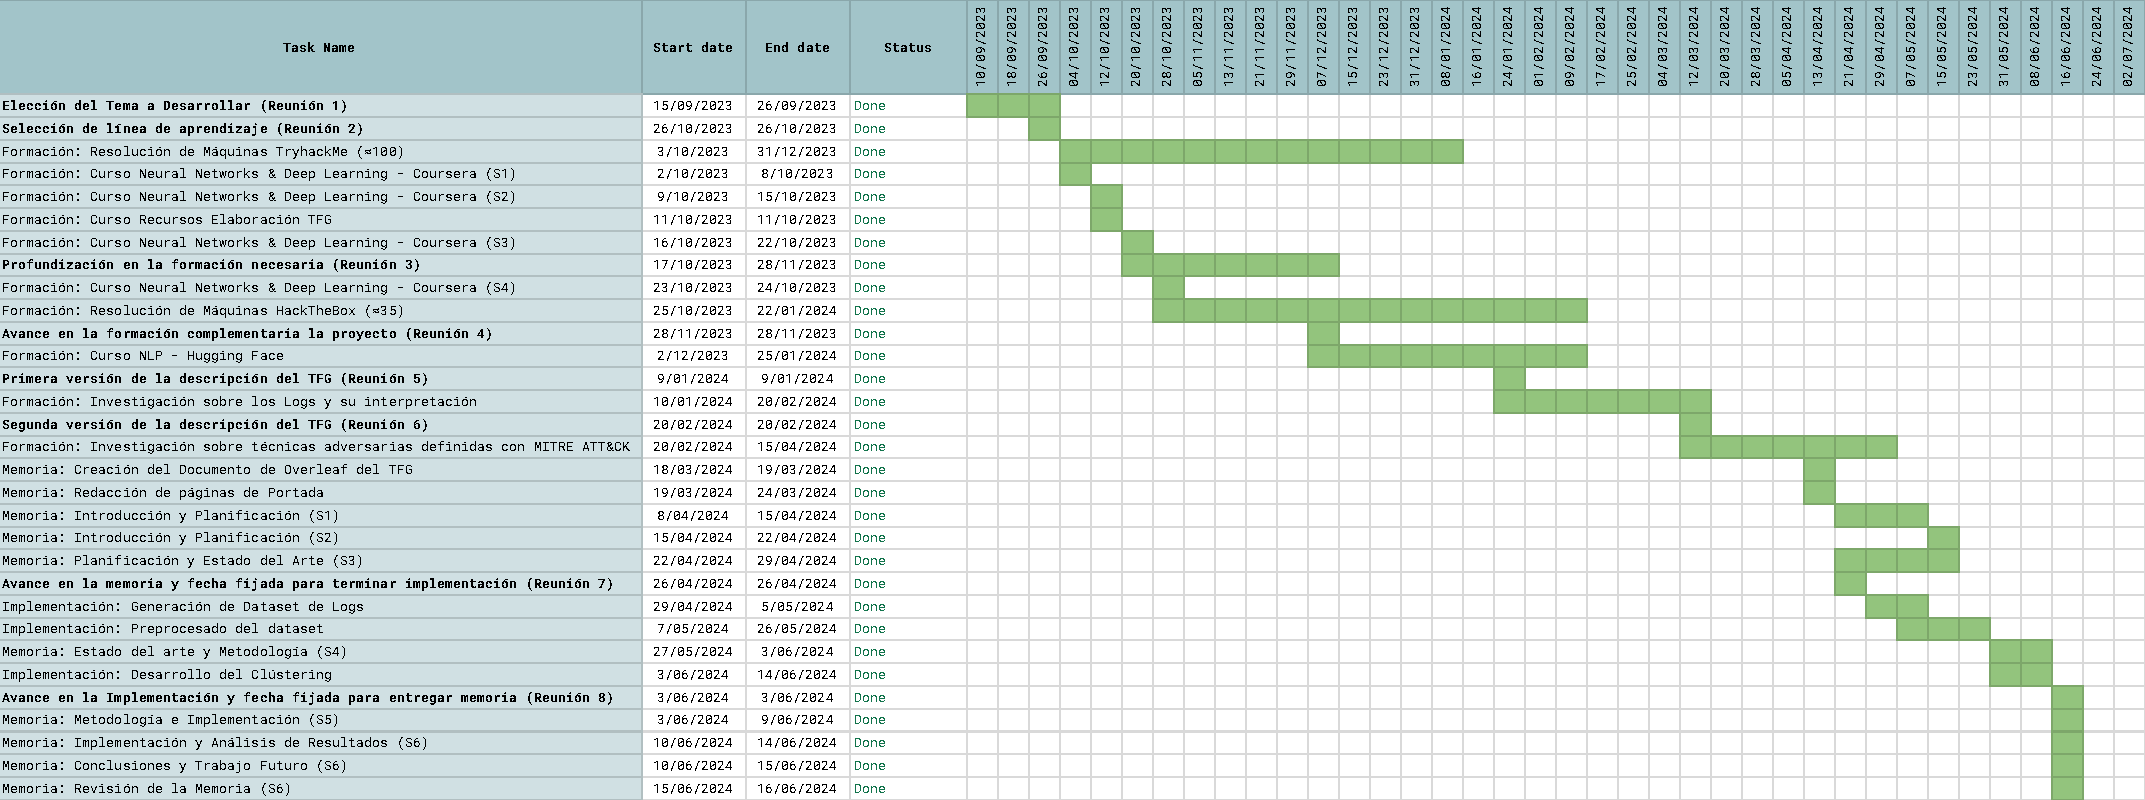
\includegraphics[width=1.3\linewidth, keepaspectratio]{imagenes/Diagrama de Gantt.png}
            \caption{Diagrama de Gantt}
            \label{fig:diagrama-gantt}
        \end{figure}
    \end{minipage}
\end{landscape}

\newpage

% ********************************************************************

\section{Presupuesto}

Para poder llevar a cabo el proyecto ha sido necesario realizar la planificación de los recursos a utilizar. En primer lugar establecer los recursos hardware, es decir, los dispositivos utilizados para el desarrollo de la memoria y de la implementación, así como los servicios de luz e internet. En segundo lugar, definir los recursos software: servicios en la nube, herramientas software, acceso a libros y artículos, etc. Finalmente, detallar el coste orientativo en recursos humanos en base al salario medio actual para un investigador en las áreas de Ciberseguridad e Inteligencia Artificial en función del tiempo invertido.

\begin{table}[H]
    \centering
    \footnotesize
    \begin{tabularx}{\linewidth}{|>{\raggedright\arraybackslash}X|r|}
    \hline
    \rowcolor{graylight}\texttt{Tipo de Recurso} & \texttt{Coste Total} \\
    \hline
    Recursos Hardware & 4.454,50\,\text{\euro} \\
    \hline
    Amortización Hardware & 411,75\,\text{\euro} \\
    \hline
    Recursos Software & 0\,\text{\euro} \\
    \hline
    Recursos Humanos & 19.545,80\,\text{\euro} \\
    \hline
    \textbf{Coste total} & \textbf{24.412,05\,\text{\euro}} \\ % Updated total cost
    \hline
    \end{tabularx}
    \caption{Presupuesto total del proyecto}
    \label{tab:presupuesto_total}
\end{table}


A continuación se desglosan cada uno de los elementos de la tabla indicando cómo se han realizado los cálculos.

\subsubsection*{Recursos Hardware}

En la siguiente tabla se detallan los recursos hardware utilizados, entre los que se incluyen un ordenador portátil y un ordenador de sobremesa, además del coste mensual para los servicios de luz e internet.

\begin{table}[H]
    \centering
    \footnotesize
    \begin{tabularx}{\linewidth}{|>{\raggedright\arraybackslash}X|c|c|c|}
    \hline
    \rowcolor{graylight}\texttt{Descripción} & \texttt{Uds.} & \texttt{Importe por unidad} & \texttt{Total} \\
    \hline
    Ordenador Portátil MSI Prestige 15 i7-1185G7 32GB RAM 1TB \gls{SSD} \gls{GTX} 1650 & 1 & 1.561,95 \euro & 1.561,95 \euro \\
    \hline
    Ordenador Sobremesa Intel i7-6700K 4.0Ghz 16GB RAM 1TB \gls{SSD} 1TB \gls{NVMe} \gls{GTX} 1080Ti 11GB \gls{GDDR}5X & 1 & 2.390,60 \euro & 2.390,60€ \\
    \hline
    Servicio de Internet (mensual) & 5 & 63,55 \euro& 317,75 \euro\\
    \hline
    Servicio de Luz (mensual) & 5 & 36,84 \euro & 184,20€ \\
    \hline
    \multicolumn{3}{|r|}{\textbf{Coste total}} & \textbf{4.454,50} \euro \\
    \hline
    \end{tabularx}
    \caption{Presupuesto hardware del Proyecto}
    \label{tab:presupuesto}
\end{table}

En base a un escenario realista, es necesario tener en cuenta la existencia de los costes de amortización. Según la normativa vigente, el porcentaje límite para la amortización de equipos de "Tratamiento de la Información y Sistemas y Programas Informáticos" se distribuye en un período de cuatro años \cite{fernandez2023amortizacion}. Considerando que el proyecto se ha desarrollado en un plazo aproximado de 5 meses, los costes de amortización serían de aproximadamente 411,75 \euro. \\

Para ello se han llevado a cabo los siguientes cálculos:

\begin{enumerate}
    \item Determinar el costo total de los equipos a amortizar:
    \[
    \text{Costo total de los equipos} = \text{Costo PC portátil} + \text{Costo PC sobremesa}
    \]
    \[
    \text{Costo total de los equipos} = 1.561,95 + 2.390,60 = 3.952,55 \ \text{\euro}
    \]

    \item Calcular la amortización anual:
    \[
    \text{Amortización anual} = \frac{\text{Costo total de los equipos}}{\text{Período de amortización en años}}
    \]
    \[
    \text{Amortización anual} = \frac{3.952,55}{4} = 988,14 \ \text{\euro}
    \]

    \item Calcular la amortización mensual:
    \[
    \text{Amortización mensual} = \frac{\text{Amortización anual}}{12}
    \]
    \[
    \text{Amortización mensual} = \frac{988,14}{12} = 82,35 \ \text{\euro}
    \]

    \item Calcular la amortización para 5 meses:
    \[
    \text{Amortización para 5 meses} = \text{Amortización mensual} \times 5
    \]
    \[
    \text{Amortización para 5 meses} = 82,35 \times 5 = 411,75 \ \text{\euro}
    \]
\end{enumerate}

\subsubsection*{Recursos Software}

En el caso de los recursos software, se ha utilizado únicamente servicios, herramientas y documentación de libre acceso. Por lo que el costo ha sido de 0€. Se ha hecho uso de los siguientes elementos:

\begin{table}[H]
    \centering
    \footnotesize
    \begin{tabularx}{\linewidth}{|l|X|}
    \hline
    \rowcolor{graylight}\texttt{Recurso} & \texttt{Detalles} \\
    \hline
    Recursos Bibliográficos & Accedidos a través de la cuenta institucional de la Universidad de Granada. Algunos ejemplos son Google Scholar, Science Direct y Scopus. \vspace{2mm}\\
    \hline
    Recursos de Internet & Accedidos a través de motores de búsqueda. Algunos ejemplos de los utilizados son Google, Firefox y DuckDuckGo. \vspace{2mm}\\
    \hline
    Conjuntos de datos & Accedidos a través de sitios web como GitHub, SecRepo y Kaggle. \vspace{2mm}\\
    \hline
    Herramientas de desarrollo & Plataformas de documentación como Overleaf e implementación como Google Colab \vspace{2mm}\\
    \hline
    \end{tabularx}
    \caption{Recursos software utilizados en el proyecto}
    \label{tab:recursos}
\end{table}

Los sistemas operativos utilizados para el desarrollo del proyecto son software libre, y están detallados en la primera sección del capítulo cinco (\ref{tab:machines}).

\subsubsection*{Recursos Humanos}

Para calcular el coste en recursos humanos, se ha considerado el salario medio de un investigador en Ciberseguridad e Inteligencia Artificial, que es de aproximadamente 30.000€ brutos anuales \cite{ufv2023cybersecurity}. El proyecto ha requerido un total de 385 horas de trabajo distribuidas en 5 meses.

\begin{enumerate}
    \item Determinar el salario mensual:
    \[
    \text{Salario mensual} = \frac{\text{Salario anual}}{12}
    \]
    \[
    \text{Salario mensual} = \frac{30.000\,€}{12} = 2.500 \ \text{\euro}
    \]

    \item Calcular el salario por hora (considerando una jornada laboral de 40 horas semanales):
    \[
    \text{Salario por hora} = \frac{\text{Salario mensual}}{160} \quad (\text{160 horas/mes})
    \]
    \[
    \text{Salario por hora} = \frac{2.500\,€}{160} = 15,63 \ \text{\euro}
    \]

    \item Calcular el coste total en recursos humanos, ajustando a un sobrecoste estimado entre un 200\% y 300\% para estudiantes:
    \[
    \text{Coste por hora (ajustado)} = \text{Salario por hora} \times 2.5
    \]
    \[
    \text{Coste por hora (ajustado)} = 15,63\,€ \times 2.5 = 39,08 \ \text{\euro} \quad (\text{Sobrecoste del 250\%})
    \]
    \[
    \text{Coste total en recursos humanos (estudiante)} = 39,08\,€ \times 385 = \textbf{15.045,80} \ \text{\euro}
    \]
\end{enumerate}

Es importante mencionar que el presupuesto asignado no es competitivo para la investigación que se quiere llevar a cabo. Generalmente, estas tareas son realizadas por expertos en la área, sin embargo este proyecto se formuló para ser ejecutado sin experiencia previa, con el principal objetivo de aprender durante el proceso. Como resultado, las tareas que un investigador experimentado podría completar en menos tiempo se extienden, lo que conlleva un aumento en los costos. \\

Además del gasto anterior, es necesario tener en cuenta el coste relativo a las horas de tutorización llevadas a cabo por los profesores asociadas a las reuniones llevadas a cabo y detalladas en el Diagrama de Gantt (\ref{fig:diagrama-gantt}), como aquellas destinadas a la corrección de esta memoria. Para realizar este cálculo deben contabilizarse las horas de esfuerzo y multiplicarse por el precio estimado por hora para un Profesor Titular de la Universidad de Granada \cite{ugr2023retribuciones}. Por tanto, este coste sería el siguiente:

\begin{enumerate}
\item Calcular el precio por hora para profesores, ajustando al sobrecoste que incluye los salarios en presupuestos:
\[
\text{Precio por hora} = 90 \text{ \euro} \quad (\text{Coste por hora típico en proyectos europeos})
\]

\item Calcular el coste total por cada profesor que tutoriza este trabajo:
\[
\text{Pablo García Sánchez} = 25 \text{ horas} \times 90 \text{ \euro / hora} = 2.250 \text{ \euro}
\]
\[
\text{Rafael Alejandro Rodríguez Gómez} = 25 \text{ horas} \times 90 \text{ \euro / hora} = 2.250 \text{ \euro}
\]
    \[
    \text{Total} = 4.500,00 \text{\euro}
    \]
\end{enumerate}

\textit{Fuente: Datos sobre retribuciones obtenidos de la Universidad de Granada} \cite{ugr2023retribuciones}.

\begin{table}[H]
    \centering
    \footnotesize
    \begin{tabularx}{\linewidth}{|>{\raggedright\arraybackslash}X|c|c|c|}
    \hline
    \rowcolor{graylight}\texttt{Descripción} & \texttt{Horas} & \texttt{Coste por hora} & \texttt{Coste Total} \\
    \hline
    Pablo García Sánchez (tutor) & 25 & 90 \text{\euro} & 2.250 \text{\euro} \\
    \hline
    Rafael Alejandro Rodríguez Gómez (cotutor) & 25 & 90 \text{\euro} & 2.250 \text{\euro} \\
    \hline
    \rowcolor{graylight}\multicolumn{3}{|r|}{\textbf{Coste total en tutorización}} & 4.500,00 \text{\euro} \\
    \hline
    \end{tabularx}
    \caption{Coste total de Recursos Humanos asociados a tutorización}
    \label{tab:coste-tutorizacion}
\end{table}

\footnotetext{Un trienio es un complemento de sueldo que se otorga por cada tres años de servicios prestados en la misma entidad, en reconocimiento a la experiencia y antigüedad acumulada.}






\chapter{Estado del Arte}

% ********************************************************************

\vspace{-0.3cm}

En este capítulo se llevará a cabo un primer acercamiento a los problemas de seguridad actuales en los sistemas Linux y se introducirán los fundamentos del marco táctico de MITRE \gls{ATT&CK}. También se realizará un análisis de las principales ventajas que está trayendo consigo el uso de la \gls{IA} para la detección de vectores de ataque, y por último se explicará cómo funcionan los \gls{SIEM} más vanguardistas.

\vspace{0.3cm}

\section{Seguridad en sistemas operativos Linux}

Las distribuciones Linux son con un 47\% \cite{linux-stats}, tal y como se indica en la gráfica de la Figura \ref{fig:linux-stats}, una de las principales elecciones para las personas que trabajan en el sector tecnológico. Son muchas las ventajas frente a sus principales competidores, como la posibilidad de adaptación y modificación tan amplia, permitiendo personalizar por completo el entorno de trabajo. Otro factor diferencial es que es de código abierto, y su descarga y uso son totalmente gratuitos, abaratando costes y permitiendo un uso escalable para las empresas e instituciones.

\begin{figure}[H]
    \vspace{-0.2cm}
    \centering
    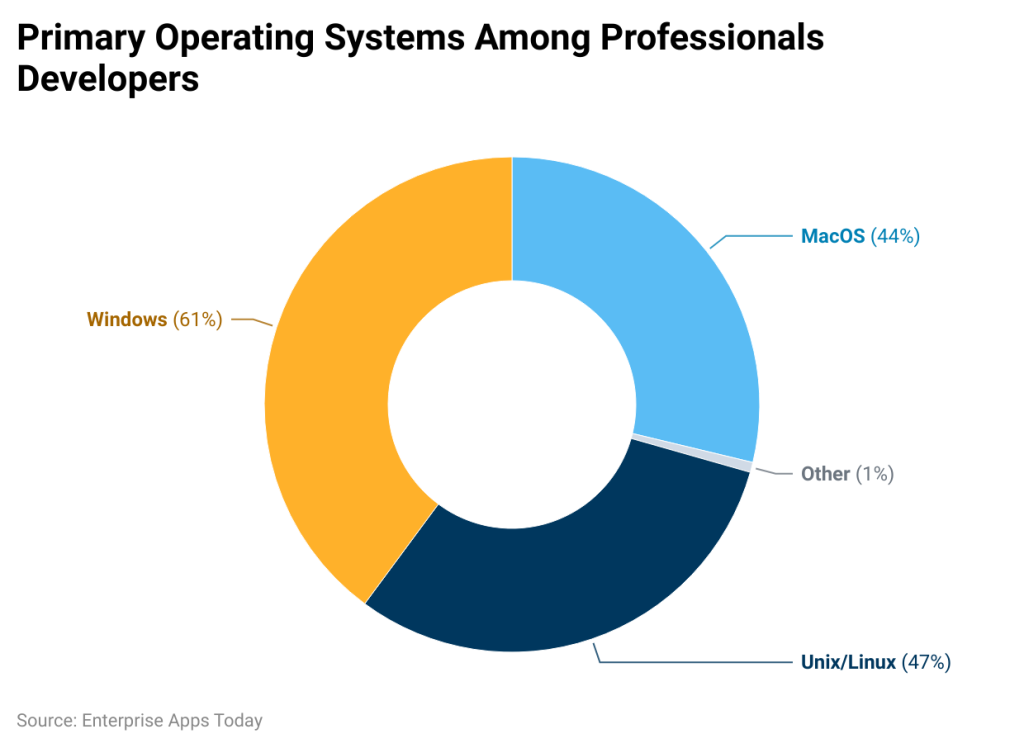
\includegraphics[scale=0.245]{imagenes/primary-operating-systems-among-professionals-developers.png}
    \caption{Comparativa entre sistemas operativos usados por profesionales \cite{linux-stats}}
    \label{fig:linux-stats}
\end{figure}

Dentro del sector de la ciberseguridad, destaca por sus distribuciones orientadas al \textit{pentesting} como \textit{Kali Linux} \cite{kali-linux}, \textit{ParrotOS} \cite{parrotsec-os} o \textit{BlackArch} \cite{blackarch-linux}. 

\vspace{-4mm}

\subsubsection*{Sistema de Archivos de Linux}

El sistema de archivos de Linux (\ref{tab:linux_file_systems}) se distingue por tener una estructura altamente organizada en base a la funcionalidad de los directorios. Entre estos, los ficheros de registro, que son críticos para la seguridad y el diagnóstico del sistema, se almacenan sistemáticamente en \texttt{/var/log}, de modo que las todas las actividades y eventos del sistema sean rastreados detalladamente y mapeados en función de una serie de características.

\begin{table}[H]
\centering
\footnotesize
\begin{tabularx}{\textwidth}{|l|X|}
\hline
\rowcolor{graylight}\texttt{Directorio} & \texttt{Descripción} \\
\hline
/bin & Binarios de comandos esenciales \\
\hline
/boot & Archivos del cargador de arranque del sistema \\
\hline
/dev & Archivos de dispositivo \\
\hline
/etc & Archivos de configuración específicos del host \\
\hline
/home & Directorio de inicio del usuario \\
\hline
/lib & Módulos de biblioteca compartida \\
\hline
/media & Archivos de medios como \textit{CD-ROM} \\
\hline
/mnt & Sistemas de archivos montados temporalmente \\
\hline
/opt & Paquetes de software de aplicaciones adicionales \\
\hline
/proc & Sistema de archivos generado automáticamente \\
\hline
/root & Directorio de inicio del usuario root \\
\hline
/run & Datos del programa en tiempo de ejecución \\
\hline
/sbin & Binarios del sistema \\
\hline
/srv & Datos específicos del sitio servidos por este sistema \\
\hline
/sys & Directorio virtual que proporciona información del sistema \\
\hline
/tmp & Archivos temporales \\
\hline
/usr & Archivos de usuario solo lectura \\
\hline
/var & Archivos que se esperan cambien continuamente \\
\hline
\end{tabularx}
\caption{Estructura del sistema de archivos de SOs basados en Linux}
\label{tab:linux_file_systems}
\end{table}

% ********************************

\subsubsection*{Gestión de permisos en Linux}

Una de las principales ventajas de los sistemas Linux es la gestión de permisos, que se desglosa en tres categorías de usuario. Este modelo divide los derechos de acceso entre el usuario (propietario del archivo), el grupo (otros usuarios que pertenecen al mismo grupo que el archivo) y otros (todos los demás usuarios del sistema). Cada archivo y directorio tiene un conjunto de permisos asociados para estas tres categorías, lo que permite un control granular sobre quién puede leer, escribir o ejecutar un archivo en el sistema.

Los permisos en Linux se identifican comúnmente como lectura (\texttt{r}), escritura (\texttt{w}) y ejecución (\texttt{x}) tal y como se indica en la siguiente tabla (\ref{tab:unix_permissions}). Además, Linux permite el uso de mecanismos avanzados como los permisos \texttt{setuid} y \texttt{setgid}, que otorgan a los programas la capacidad de ejecutarse con los privilegios de otro usuario o grupo, respectivamente. Estos permisos se pueden asignar por medio del comando \texttt{chmod} \cite{chmod-quickref}. Además, los permisos también pueden estar asociados a un fichero específico o a su nivel de pertenencia (\ref{tab:file_types_owners}).

\begin{center}
    \begin{mdframed}
    \scriptsize
            \begin{minted}{bash}
-rwxr-xr-- 22 root 4096 2024-03-03 18:09 file.txt
            \end{minted}
    \end{mdframed}
\end{center}

En este ejemplo, el archivo tiene:
\begin{itemize}
    \item Permisos de lectura, escritura y ejecución para el usuario propietario (rwx)
    \item Permisos de lectura y ejecución para el grupo (r-x)
    \item Solo permisos de lectura para otros usuarios (r--)
\end{itemize}

\begin{table}[H]
\footnotesize
\centering
\renewcommand{\arraystretch}{1.5}
\begin{tabularx}{\textwidth}{|c|c|X|}
\hline
\rowcolor{graylight}\texttt{Abreviatura} & \texttt{Valor} & \textt{Acción} \\
\hline
r & 4 & Lectura \\
w & 2 & Escritura \\
x & 1 & Ejecución \\
- & 0 & Sin permiso \\
\hline
\end{tabularx}
\caption{Estructura de permisos en Sistemas Linux \cite{chmod-quickref}}
\label{tab:unix_permissions}
\end{table}


\begin{table}[H]
\footnotesize
\centering
\renewcommand{\arraystretch}{1.5}
\begin{tabularx}{\textwidth}{|c|X|c|X|}
\hline
\rowcolor{graylight}\texttt{Quién} & \texttt{Significado} & \texttt{Tipo de Archivo Abreviatura} & \texttt{Tipo de Archivo} \\
\hline
u & Usuario & d & Directorio \\
g & Grupo & - & Archivo regular \\
o & Otros & l & Enlace simbólico \\
a & Todos (\texttt{ugo}) & - & -- \\
\hline
\end{tabularx}
\caption{Tipos y propietarios de archivos en Sistemas Linux \cite{chmod-quickref}}
\label{tab:file_types_owners}
\end{table}


Es crucial implementar la política de mínima permisibilidad en la gestión de permisos para minimizar los riesgos de ataques que exploten las estructuras de permisos laxos. Limitar el acceso a la información y funcionalidades del sistema solo a quienes realmente lo necesitan ayuda a proteger contra amenazas internas y externas, y es especialmente importante para evitar que los ataques se propaguen a través de la cadena de mando en un organigrama empresarial.

% ********************************

\subsection{\textit{Hardening} del sistema}

Existen una serie de medidas básicas de seguridad \cite{urrego2023seguridad} para añadir una capa de protección a los Sistemas Linux, y que desgraciadamente no suelen llevarse a cabo por desconocimiento, incluso por aquellos profesionales que despliegan sus servidores y acaban siendo atacados a causa de este motivo. Entre estas medidas, destacan:

\begin{enumerate}[label=\Alph*.,itemsep=2pt,parsep=1pt]
    \item \texttt{Configuración de conexión remota SSH:} cambiar el puerto predeterminado, sustituir el acceso por contraseña por el uso de pares de claves publica-privada y deshabilitar el acceso root directo.
    \vspace{1mm}
    \item \texttt{Listar puertos abiertos:} revisar y filtrar los puertos abiertos para mantener solo los necesarios para la operación segura del sistema. \\
    \item \texttt{Habilitar IPTABLES:} configuración de un \textit{firewall} para controlar el acceso a los servicios según las necesidades de seguridad. \\
    \item \texttt{Prevención de Ataques \gls{DDoS}} (\textit{Distributed Denial-of-Service}): implementación de medidas para mitigar ataques de este tipo, como limitar conexiones y usar SYN cookies. \\
    \item \texttt{Software Instalado:} gestión de los paquetes instalados para asegurar que solo se mantengan los necesarios y se evite software no confiable. \\
    \item \texttt{Actualización Kernel y Parches de Seguridad:} mantener el sistema actualizado con los últimos parches de seguridad para proteger contra vulnerabilidades conocidas. \\
    \item \texttt{Password aging:} implementación de políticas de caducidad y renovación de contraseñas para mejorar la seguridad de las cuentas. \\
    \item \texttt{Encriptación de disco duro:} aplicación de cifrado al nivel de disco para proteger los datos en caso de acceso físico no autorizado. \\
    \item \texttt{Antivirus:} uso de software antivirus para detectar y prevenir malware y otros tipos de software malicioso. \\
    \item \texttt{Uso de \gls{VPN}} (\textit{Virtual Private Network}): conexión a redes privadas virtuales para asegurar las conexiones remotas y proteger los datos en tránsito. \\
    \item \texttt{Servidor de archivos \gls{NFS}:} configuración segura de servidores de archivos en red para compartir recursos dentro de una red de confianza. \\
    \item \texttt{Habilitar \texttt{\gls{SUDO}}:} control de los privilegios de ejecución de comandos para limitar las operaciones que los usuarios pueden realizar. \\
    \item \texttt{Backups:} implementación de copias de seguridad cronológicas para proteger los datos frente a pérdidas accidentales o maliciosas. \\
    \item \texttt{Monitorización y manejo de \textit{logs}:} revisión y análisis de \textit{logs} para detectar actividades inusuales y potenciales brechas de seguridad.
\end{enumerate}

De todas las medidas anteriores, este proyecto estará enfocado en la última: monitorización y manejo de \textit{logs}, con el fin de detectar posible patrones de ataque en base al análisis de los eventos registrados en un sistema o conjunto de sistemas Linux. Igualmente, cada una de ellas representan una capa de robustez en el nivel de seguridad de equipo, por lo que su importancia debe ser tenida en cuenta.

% ********************************

\vspace{-0.3cm}

\subsection{Generación y monitorización de logs}

Los logs son ficheros que registran actividades realizadas en un sistema o servicio. Por consiguiente, estos pueden llegar a ser nuestros principales aliados para detectar intentos de acceso no autorizados, manipulación de datos o incluso intentos de intrusión. Además, proporcionan evidencia crucial en caso de incidentes de seguridad, ayudando en las investigaciones forenses digitales.

Existen diversas herramientas y soluciones para la generación, monitorización y gestión de \textit{logs} que automatizan y facilitan estas tareas. Entre las más destacadas se encuentran: \\

\texttt{\gls{ELK} Stack} (\textit{Elasticsearch, Logstash, y Kibana}) \cite{elastic-stack}: esta suite de herramientas permite la recopilación, indexación, y visualización de \textit{logs} de manera eficiente y escalable. \textit{Elasticsearch} indexa los \textit{logs}, \textit{Logstash} los procesa y \textit{Kibana} proporciona una interfaz gráfica para explorar y visualizar los datos.

\texttt{Splunk} \cite{splunk}: otra solución popular que CISCO \cite{cisco} ofrece con capacidades avanzadas de recogida, indexación y análisis de grandes volúmenes de datos en tiempo real. \textit{Splunk} es particularmente apreciado por su potente interfaz de búsqueda y visualización.

\texttt{Zabbix} \cite{zabbix}: además de monitorizar el rendimiento y la disponibilidad, Zabbix es capaz de recoger y analizar \textit{logs} de diversos sistemas y dispositivos, ofreciendo una solución integral para el seguimiento de infraestructuras \gls{IT}. 

\texttt{Syslog} es, según el \texttt{\gls{RFC} 5424} \cite{rfc5424} , una de las herramientas más antiguas y ampliamente utilizadas para la gestión de \textit{logs} en sistemas GNU/Linux. Permite la centralización de \textit{logs} de múltiples sistemas en un servidor \texttt{syslog}. Utiliza niveles de prioridad asignados a los mensajes:

\begin{table}[H]
\centering
\footnotesize
\begin{tabular}{|c|c|p{8.5cm}|}
\hline
\rowcolor{graylight}\texttt{Valor} & \texttt{Prioridad} & \texttt{Descripción} \\
\hline
0 & Emergency & El sistema no se puede usar \\
\hline
1 & Alert & Se debe actuar inmediatamente \\
\hline
2 & Critical & Condiciones críticas \\
\hline
3 & Error & Condiciones de error \\
\hline
4 & Warning & Condiciones de advertencia \\
\hline
5 & Notice & Condición normal pero significativa \\
\hline
6 & Info & Mensajes informativos \\
\hline
7 & Debug & Mensajes de nivel de depuración \\
\hline
\end{tabular}
\caption{Niveles de prioridad de syslog}
\label{tab:syslog_priority}
\end{table}

Además, hace uso de las llamadas \textit{facilities}, una serie de categorías predefinidas que clasifican los logs en función de la parte del sistema operativo que las ha generado, ayudando a organizar los mensajes para facilitar su filtrado y procesamiento.

\newpage

\begin{table}[H]
\centering
\footnotesize
\begin{tabular}{|c|l|p{8cm}|}
\hline
\rowcolor{graylight}\texttt{Código } & \texttt{Keyword} & \texttt{Descripción} \\
\hline
0 & kern & Mensajes del kernel \\
\hline
1 & user & Mensajes a nivel de usuario \\
\hline
2 & mail & Sistema de correo \\
\hline
3 & daemon & Demonios del sistema \\
\hline
4 & auth & Mensajes de seguridad/autenticación \\
\hline
5 & syslog & Mensajes generados internamente por syslogd \\
\hline
6 & lpr & Subsistema de impresora de línea \\
\hline
7 & news & Subsistema de noticias de red \\
\hline
8 & uucp & Subsistema \gls{UUCP} (\textit{Unix to Unix Copy Protocol}) \\
\hline
9 & cron & Subsistema cron \\
\hline
10 & authpriv & Mensajes de seguridad/autenticación privados \\
\hline
11 & ftp & Demonio \gls{FTP} (\textit{File Transfer Protocol}) \\
\hline
12 & ntp & Subsistema \gls{NTP} (\textit{Network Time Protocol}) \\
\hline
13 & security & Auditoría de logs \\
\hline
14 & console & Alerta de logs \\
\hline
15 & solaris-cron & Demonio de planificación \\
\hline
16–23 & local0 – local7 & Facilities usados localmente \\
\hline
\end{tabular}
\caption{\textit{Facilities} de Syslog}
\label{tab:syslog_facilities}
\end{table}

Las implementaciones de \verb|syslog| varían y están adaptadas para diferentes distribuciones de Linux. Por ejemplo, \verb|rsyslog| es más común en distribuciones basadas en Debian, mientras que \verb|syslog-ng| \footnotemark es ampliamente utilizado en distribuciones basadas en RedHat.

Entre las ventajas de \verb|rsyslog| se encuentra su capacidad para manejar grandes volúmenes de datos. Por otro lado, \verb|syslog-ng| destaca por su capacidad de \textit{parsing} y filtrado de \textit{logs} antes de su almacenamiento, lo que facilita una organización más eficiente y una mejor detección de problemas.

\footnotetext{Donde ng hace referencia a \textit{new-generation}}

Según se observa en la Figura \ref{fig:varlog}, estos ficheros se encuentran comúnmente en la ruta \verb|/var/log|, algunos de ellos en subcarpetas asociadas a servicios o programas específicos que cuentan con su propio sistema de monitorización. En cuanto a la nomenclatura utilizada para los ficheros, hay varios que tienen el mismo nombre seguido de la expresión regular \verb|<name>.log.*| donde * es un número que aumenta secuencialmente. Esto se debe a que cuando se completa el espacio máximo utilizable de un fichero se genera otro nuevo con ese mismo tamaño utilizable. Por ejemplo, en el caso de \verb|boot.log| o de \verb|dpkg.log|.

\begin{figure}[H]
    \centering
    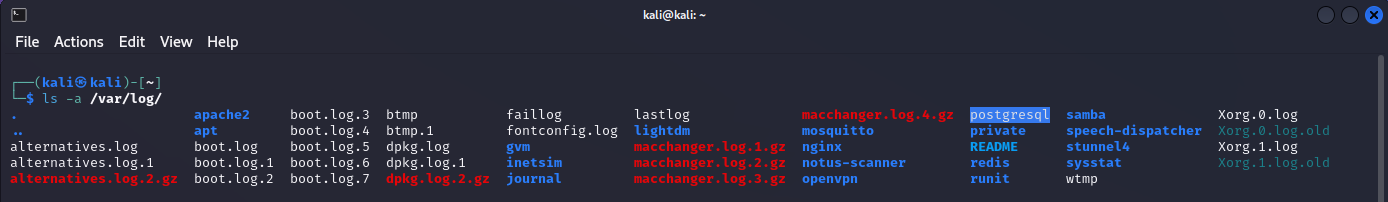
\includegraphics[width=\textwidth]{imagenes/var-log.png}
    \caption{Contenido del registro de \textit{/var/log}}
    \label{fig:varlog}
\end{figure}

\newpage

Los logs pueden presentar diferencias en base a la información que almacenan, al formato y al orden en el que la representan, de modo que inicialmente no resulta sencillo trabajar con dos tipos de ficheros \textit{log} de diferentes formatos. En las siguientes Figuras, se muestra el contenido de \verb|auth.log| y de \verb|dpkg.log| (\ref{fig:auth-log} y \ref{fig:dpkg-log} respectivamente):

\begin{figure}[H]
\centering
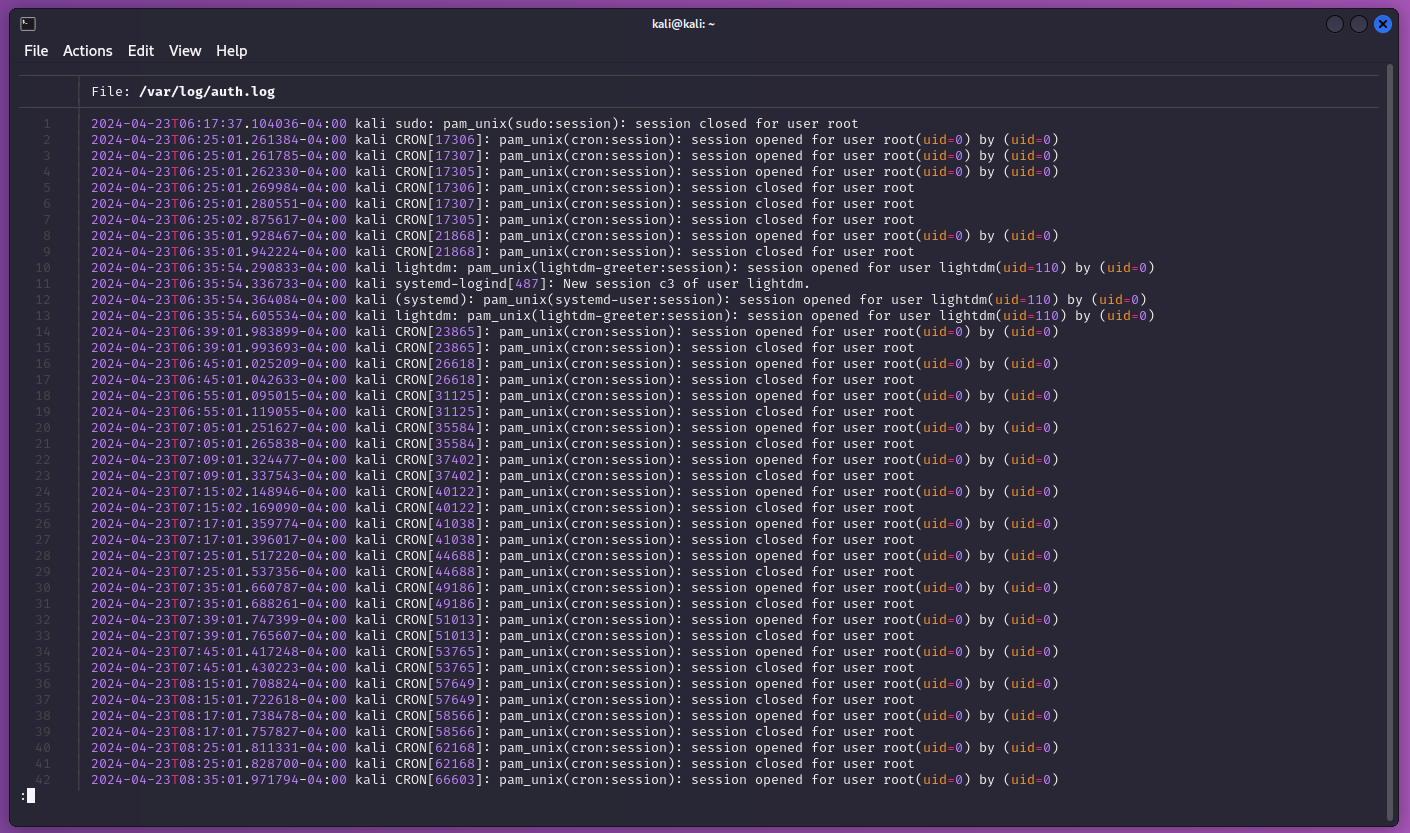
\includegraphics[width=\linewidth]{imagenes/log-structure.png}
\captionof{figure}{Contenido del registro de \textit{auth.log}}
\label{fig:auth-log}
\end{figure}

\begin{figure}[H]
    \centering
    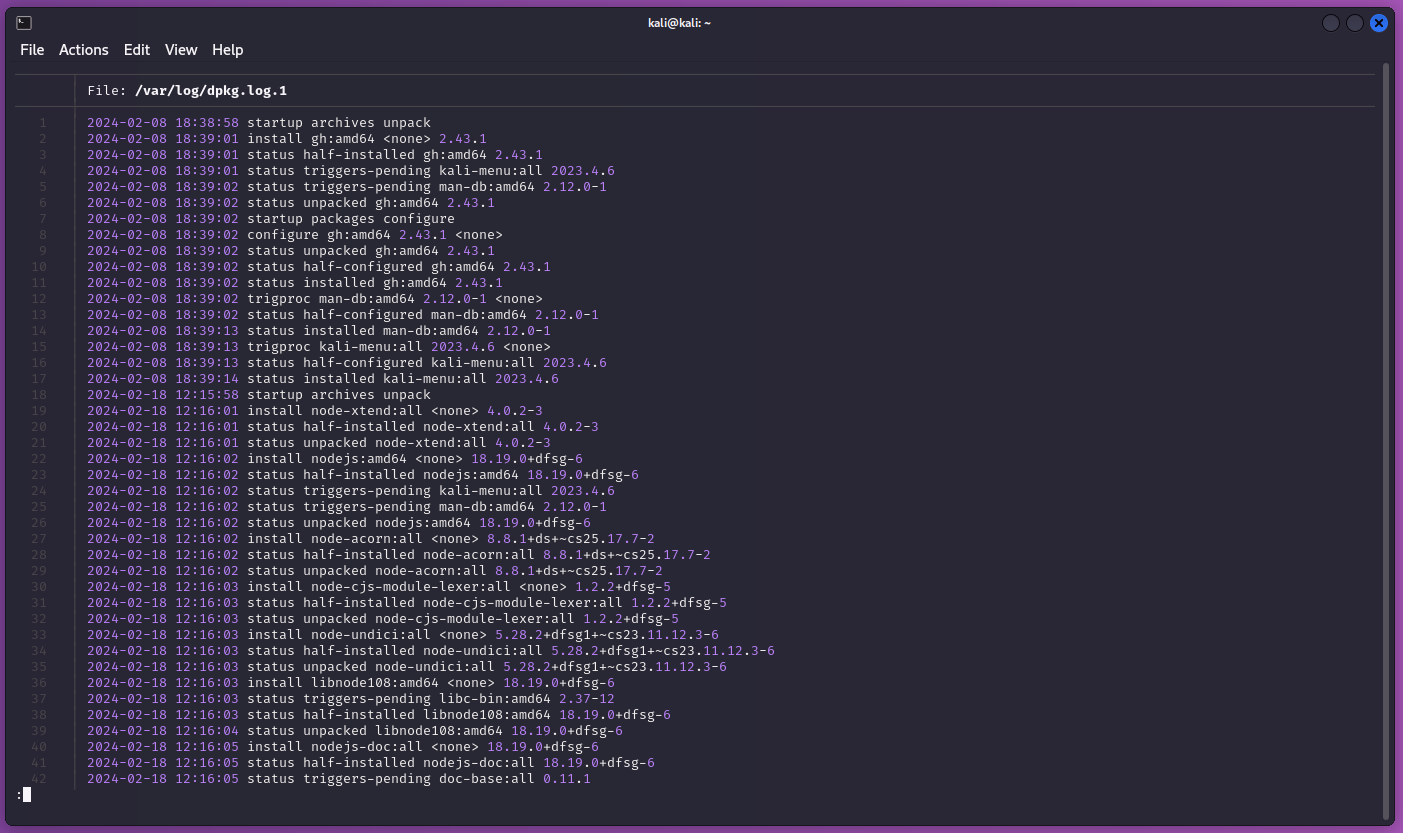
\includegraphics[width=\linewidth]{imagenes/log-structure-2.png}
    \caption{Contenido del registro de \textit{dpkg.log}}
    \label{fig:dpkg-log}
\end{figure}

\newpage

En estos ejemplos, ambos ficheros contienen los campos \textit{timestamp}, es decir, la fecha y la hora a la que sucedió cada evento, y \textit{message}, pero propiedades como la separación entre campos o la precisión que presentan son distintas. A pesar de estas diferencias, la información puede llegar a combinarse a través de técnicas de preprocesamiento de modo que sea utilizable dentro de un mismo formato de \textit{datasets}. 

Además de los ficheros comentados anteriormente, existen otras herramientas importantes para el manejo de \textit{logs} en Linux que contribuyen al análisis de seguridad y al diagnóstico de problemas:

\begin{itemize}
    \item \verb|dmesg|: muestra mensajes del kernel útiles para diagnosticar problemas de hardware y de carga de controladores durante el arranque (puede visualizarse en la Figura \ref{fig:dmesg}).
    \item \verb|journalctl|: herramienta para consultar y administrar \textit{logs} del sistema gestionados por \verb|systemd| (puede visualizarse en la Figura \ref{fig:journalctl}).
\end{itemize}

\begin{figure} [H]
    \centering
    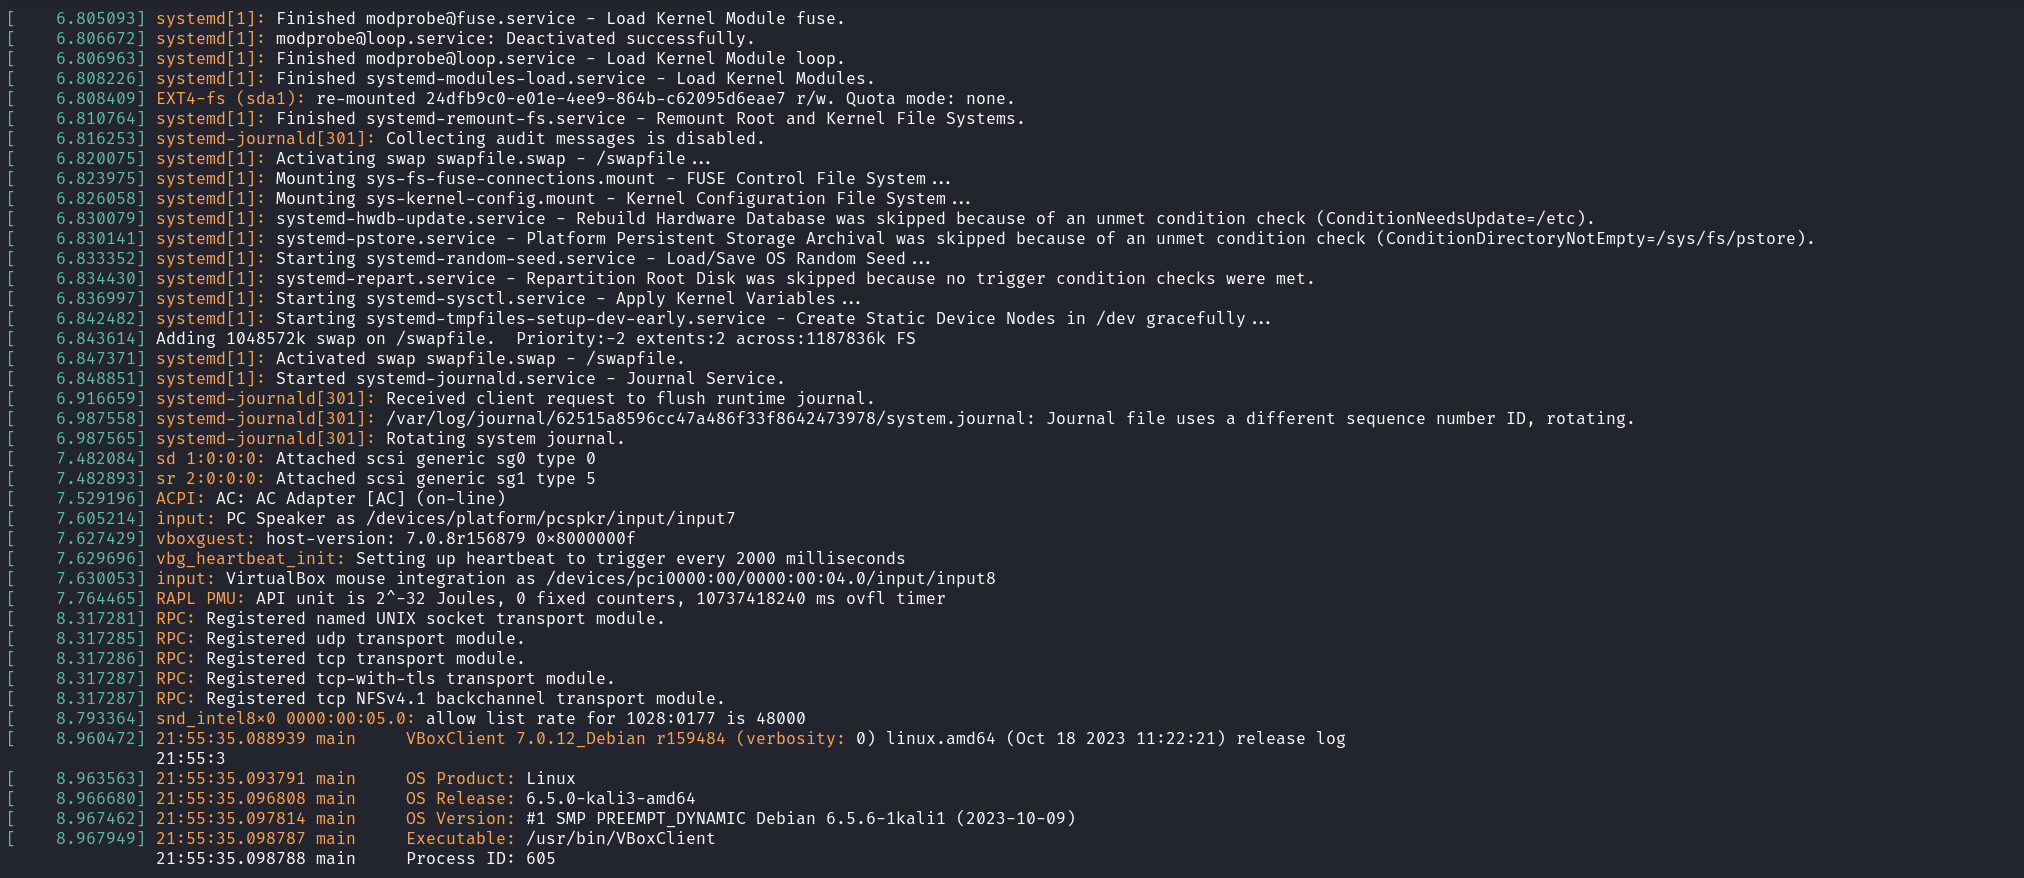
\includegraphics[width=1\linewidth]{imagenes/dmesg.png}
    \caption{Contenido de los logs de \textit{dmesg}}
    \label{fig:dmesg}
\end{figure}

\begin{figure}[H]
    \centering
    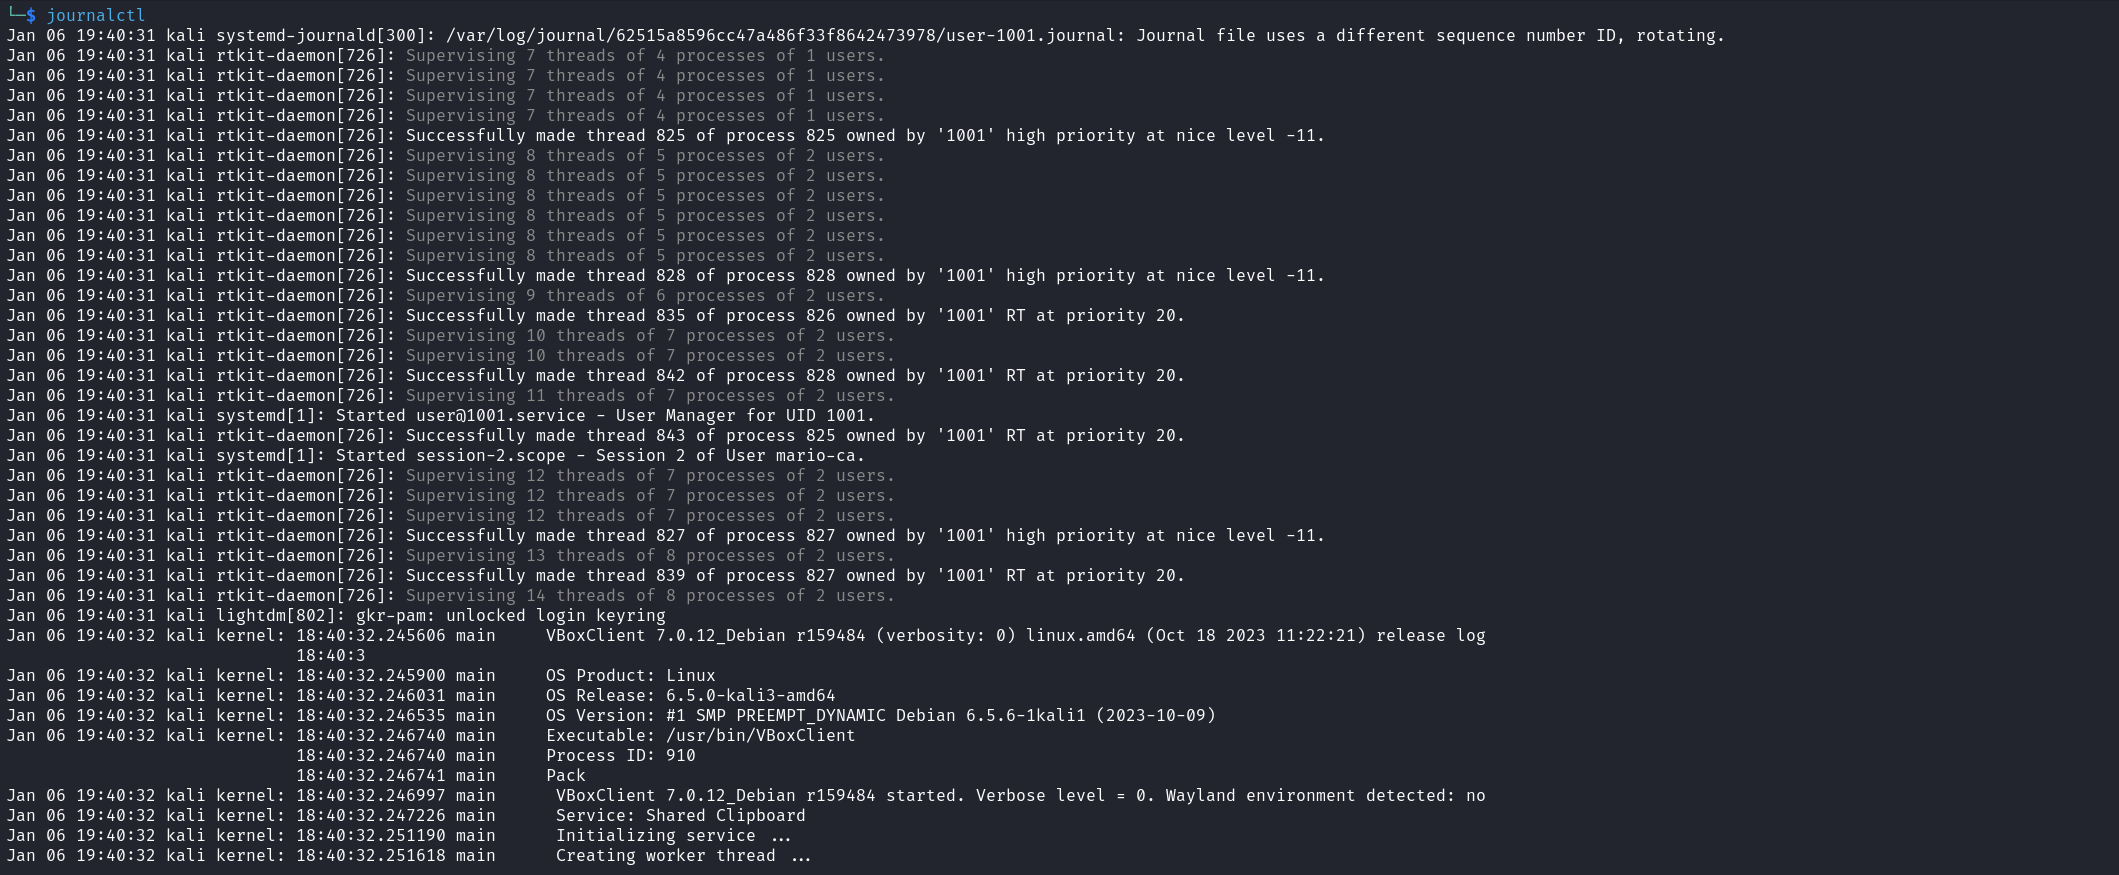
\includegraphics[width=1\linewidth]{imagenes/journalctl.png}
    \caption{Contenido de los logs de \textit{journalctl}}
    \label{fig:journalctl}
\end{figure}

% ********************************

\newpage

% ********************************************************************

\section{El marco de MITRE ATT\&CK}

Con el fin de proporcionar una guía detallada y práctica que permita entender y combatir mejor los ciberataques, nació en 2013 \cite{10005490} el marco de técnicas adversarias de MITRE \gls{ATT&CK} (\textit{Adversarial Tactics, Techniques, and Common Knowledge}). Este fue creado por el \gls{NIST}, y clasifica las diferentes \gls{TTP}s (\textit{Tactics, Techniques and Procedures}) seguidas por los cibercriminales en cada una de las fases de un ataque.

\vspace{-1mm}

\begin{itemize}
    \item \textbf{Tácticas}: Describen el \textit{qué} y el \textit{porqué} de las acciones de los adversarios, refiriéndose a su objetivo general y estrategia durante un ataque.
    \item \textbf{Técnicas}: Revelan el \textit{cómo}, especificando el método específico empleado para alcanzar un objetivo táctico.
    \item \textbf{Procedimientos}: Son los \textit{detalles exactos} de la técnica utilizada, incluyendo los comandos ejecutados, la secuencia de operaciones y cualquier configuración aplicada.
\end{itemize}

\vspace{-1mm}

Por ejemplo, en un ataque de \textit{phishing}, la \textbf{táctica} empleada sería la recopilación inicial de acceso, la técnica podría ser el envío de correos electrónicos engañosos y por último el \textbf{procedimiento} consistiría en el uso de un correo electrónico que aparenta ser una alerta legítima de seguridad de una institución conocida para engañar a los usuarios y hacer que revelen sus credenciales.

MITRE \gls{ATT&CK} está compuesto por una lista estructurada de comportamientos expresados en forma matricial que, tal y como se ilustra en la Figura \ref{fig:mitre-matrix}, proporcionan una taxonomía común de acciones tanto del propio adversario como de contra-medidas para defenderse del mismo.

\vspace{-1mm}

\begin{figure}[H]
    \centering
    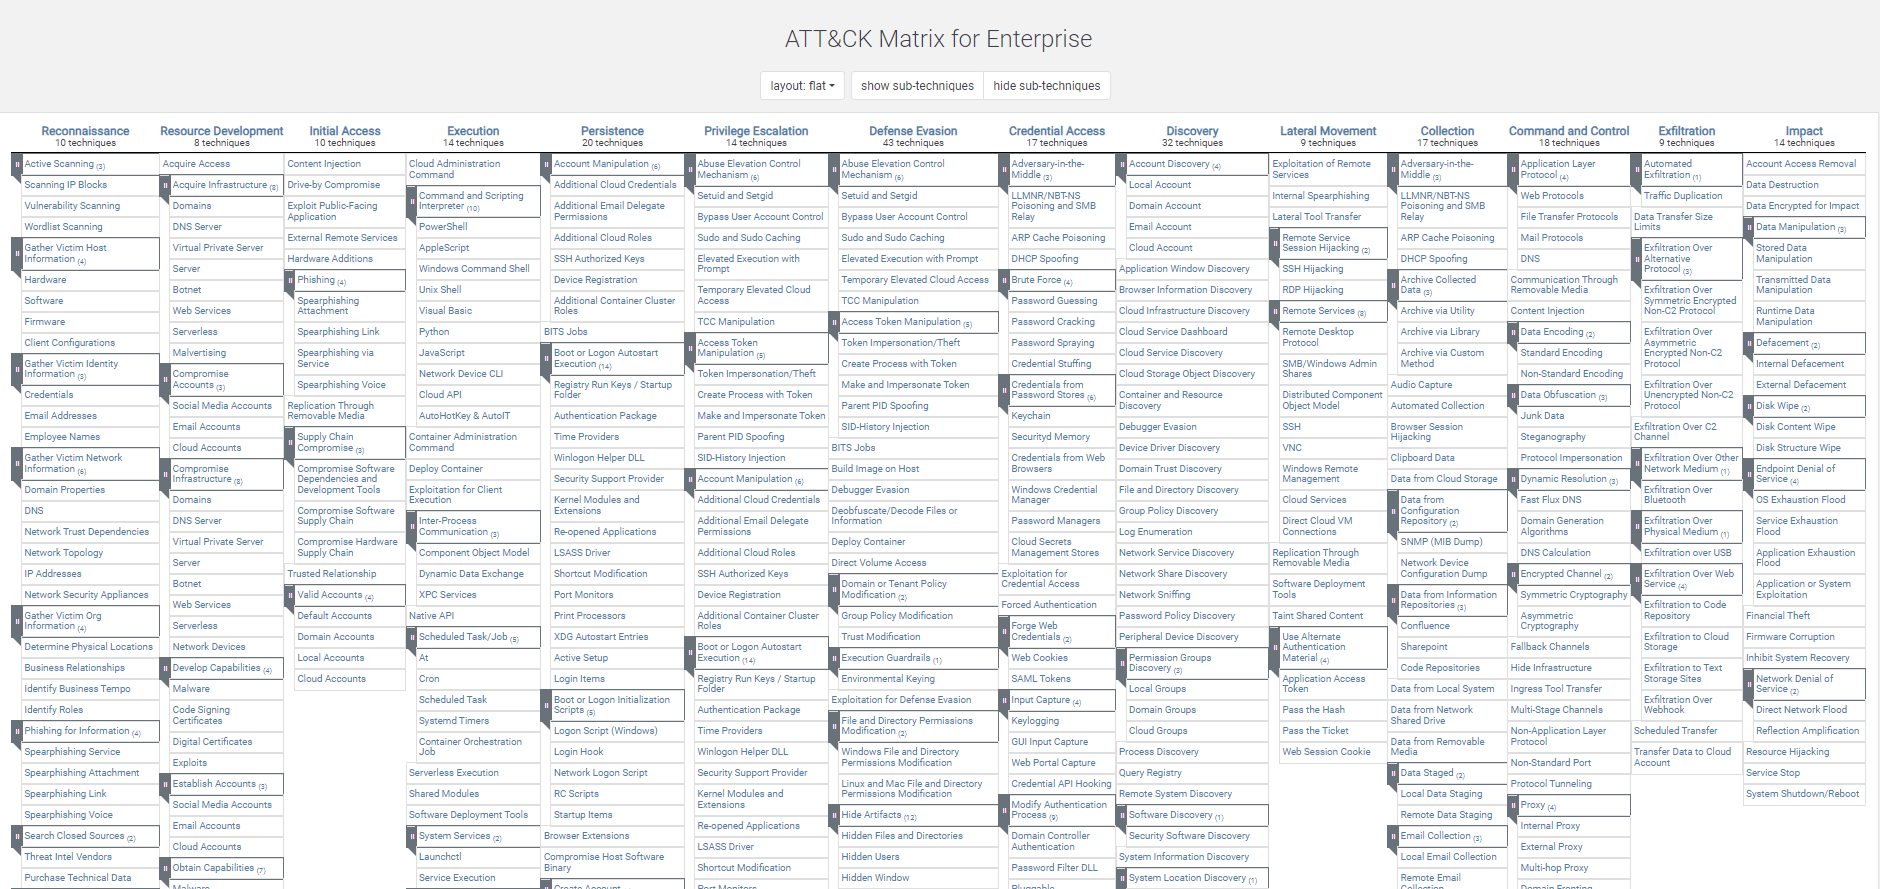
\includegraphics[width=\textwidth]{imagenes/mitre-matrix.png}
    \caption{Matriz de técnicas y tácticas de MITRE ATT\&CK para enterprise \cite{mitre_attack}}
    \label{fig:mitre-matrix}
\end{figure}

\vspace{-2.5mm}

Actualmente es muy utilizado tanto a nivel empresarial como gubernamental a modo de modelo base para el desarrollo de productos y servicios de ciberseguridad. La principal causa de su éxito podría ser la forma en la que se describe cada procedimiento de forma detallada y con una terminología correcta y entendible, pero sin llegar a mencionar el uso de herramientas especificas que lleven a cabo las acciones descritas. 

\newpage

Una gran ventaja de MITRE ATT\&CK \cite{mitre_attack} es que se encuentra en una constante evolución, incorporando a la matriz técnicas y sub-técnicas vanguardistas que van apareciendo en la escena del cibercrimen. Cada una de las técnicas y sub-técnicas \ref{sec:técnicas} de la matriz de MITRE está asociada a un identificador único y cuenta con su correspondiente descripción, además de otra información de relevancia como un listado de formas de mitigación y/o detección. 

Estos identificadores se estructuran siguiendo un patrón muy similar: uno o dos caracteres seguidos de cuatro dígitos. Esta forma de identificarlos permite reservar el suficiente espacio como para añadir durante muchos años nuevas tácticas, técnicas, sub-técnicas, procedimientos, etc.

\begin{table}[h]
\centering
\footnotesize
\begin{tabular}{|c|l|p{8cm}|}
\hline
\rowcolor{graylight}\texttt{Identificador} & \texttt{Categoría} & \texttt{Descripción} \\
\hline
\texttt{TA\#\#\#\#} & Tácticas & TA indica que es un identificador de táctica y va seguido de 4 dígitos. Ejemplo: \texttt{TA0001}. \\
\hline
\texttt{T\#\#\#\#} & Técnicas & T indica que es un identificador de técnica y va seguido de 4 dígitos. Ejemplo: \texttt{T1059}. \\
\hline
\texttt{T\#\#\#\#.\#\#\#} & Sub-técnicas & Parecido a los identificadores de técnicas, pero cuentan con caracteres adicionales ya que se agrupan dentro de los anteriores. Ejemplo: \texttt{T1059.001}. \\
\hline
\texttt{M\#\#\#\#} & Mitigaciones & M indica que es un identificador de mitigación y va seguido de 4 dígitos. Ejemplo: \texttt{M1050}. \\
\hline
\texttt{DS\#\#\#\#} & Detecciones & DS indica que es un identificador de detección y va seguido de 4 dígitos. Ejemplo: \texttt{DS0029}. \\
\hline
\texttt{S\#\#\#\#} | \texttt{G\#\#\#\#} & Procedimientos & Identificadores de procedimientos específicos usados por actores de amenazas o grupos específicos. Ejemplo: \texttt{S0003} para procedimientos y \texttt{G0007} para grupos. \\
\hline
\end{tabular}
\caption{Identificadores del marco de \textit{MITRE ATT\&CK}}
\label{tab:mitre_attack_identifiers}
\end{table}

Hace relativamente poco, se publicaron versiones más específicas de esta matriz tanto para móviles como para \gls{ICS} (\textit{Industrial control system}). Estas contienen menos volumen de tácticas y técnicas pero se adaptan mejor a un escenario real de ataque sobre este tipo de entornos. Además, desde MITRE han desarrollado también matrices específicas para distintos Sistemas Operativos y áreas de conocimiento, también más pequeñas pero más precisas al entorno de simulación.

\begin{table}[h!]
    \footnotesize
    \centering
    \begin{tabularx}{\linewidth}{|l|X|} % Cambio de tipo de columna para mejor control sobre el ancho de la primera columna
        \hline 
        \footnotesize \rowcolor{graylight}\texttt{Categoría} & \footnotesize \texttt{Plataformas / Sistemas} \\ 
        \hline
        \footnotesize \texttt{Enterprise} & 
        \begin{tabular}[t]{@{}l@{}}
            PRE \\
            Windows \\
            macOS \\
            Linux \\
            Cloud \\
            Network \\
            Containers \\
        \end{tabular} \\
        \hline
        \footnotesize \texttt{Mobile} &
        \begin{tabular}[t]{@{}l@{}}
            Android \\
            iOS \\
        \end{tabular} \\
        \hline
        \footnotesize \texttt{ICS} & 
        \begin{tabular}[t]{@{}l@{}}
            \gls{PLC}, \gls{RTU}, \gls{SCADA}, \gls{DCS} 
        \end{tabular} \\
        \hline
    \end{tabularx}
    \caption{Matrices de MITRE ATT\&CK}
    \label{tab:mitre_attack_matrices}
\end{table}


En el caso de este proyecto se hará uso de la matriz de Linux ya que es la que mejor se adapta al escenario donde se llevarán a cabo las simulaciones de ataques.

\subsection{Tácticas} \label{sec:tacticas}

MITRE ATT\&CK  \cite{mitre_attack} agrupa las distintas técnicas de intrusión dentro de catorce tácticas distintas ordenadas secuencialmente, aunque este orden puede orden variar en determinadas operaciones.

\begin{table}[H] 
\centering
\footnotesize
\begin{tabular}{|c|l|p{8cm}|}
\hline
\rowcolor{graylight}\texttt{Código} & \texttt{Fase del Ataque} & \texttt{Descripción} \\
\hline
1 & Reconocimiento & Recopilación de información para la planificación futura un ataque. \\
\hline
2 & Desarrollo de recursos & Creación de recursos que respalden el desarrollo de un ataque. \\
\hline
3 & Acceso inicial & Intento inicial de acceder al objetivo a comprometer. \\
\hline
4 & Ejecución & Introducción de código malicioso en el sistema atacado. \\
\hline
5 & Persistencia & Asentar un acceso continuo al sistema objetivo a través de reinicios, cambios de credenciales y supresión de interrupciones que podrían cancelar su acceso. \\
\hline
6 & Escalada de privilegios & Obtención de permisos de nivel superior para poder acceder a más recursos del sistema atacado. \\
\hline
7 & Evasión de defensa & Ocultación frente a la detección mientras se está efectuando la operación de compromiso. \\
\hline
8 & Acceso a credenciales & Robo de credenciales para acceder al sistema de destino. \\
\hline
9 & Descubrimiento & Obtención de más conocimientos sobre el sistema objetivo y su entorno. \\
\hline
10 & Movimiento lateral & Desplazamiento a través del entorno interno del conjunto de sistemas objetivo. \\
\hline
11 & Recopilación & Búsqueda de información relevante del objetivo. \\
\hline
12 & \gls{C2} - Command \& Control & Comunicación remota con el sistema comprometido para controlar y operar sobre este. \\
\hline
13 & Exfiltración & Robo de datos sensibles almacenados en el sistema comprometido. \\
\hline
14 & Impacto & Manipulación, ocultación o destrucción del sistema comprometido y sus datos. \\
\hline
\end{tabular}
\caption{Conjunto de tácticas ofensivas del marco de \textit{MITRE ATT\&CK}}
\label{tab:mitre_attack_phases}
\end{table}

\subsection{Técnicas} \label{sec:técnicas}

Cada una de las tácticas indicadas en la subsección anterior (\ref{sec:tacticas}) contiene un listado técnicas que pueden utilizarse para llevar a cabo cada objetivo. Estas técnicas a su vez agrupan una serie de subtécnicas, proporcionando un mayor nivel de abstracción que aglutine una mayor base de conocimiento con respecto a todas las formas de llevar a cabo una acción. 

Todo esto puede resultar inicialmente algo confuso de entender, por lo que una manera útil de comprenderlo es imaginarlo como una especie de matriz tridimensional en la que cada táctica es una fila (abscisas), cada técnica una columna (ordenadas) y por último cada subtécnica una altura o cota. Por ejemplo, dentro de la táctica de Reconocimiento (\ref{tab:mitre_attack_phases}) existen actualmente diez técnicas distintas, cada una de ellas con una serie de subtécnicas más específicas.

\begin{figure}[H]
    \centering
    \begin{minipage}[b]{0.45\textwidth}
        \centering
        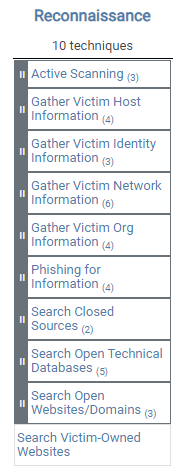
\includegraphics[width=25mm]{imagenes/techniques.png}
        \caption{Listado de técnicas de la táctica de \textit{Reconnaissance} \cite{mitre_attack}}
        \label{fig:reconnaissance-techniques}
    \end{minipage}
    \hspace{0.05\textwidth} % Espacio horizontal entre las dos minipages
    \begin{minipage}[b]{0.45\textwidth}
        \centering
        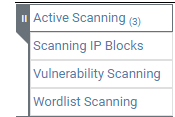
\includegraphics[width=5cm]{imagenes/active-scanning.png}
        \caption{Sub-técnicas de \textit{Active Scanning} \cite{mitre_attack}}
        \label{fig:active-scanning}
    \end{minipage}
\end{figure}


Según se ilustra en las Figuras \ref{fig:reconnaissance-techniques} y \ref{fig:active-scanning}, la primera técnica de la táctica de Reconocimiento, \textit{Active Scanning}, cuenta con 3 subtécnicas: \textit{Scanning IP Blocks}, \textit{Vulnerability Scanning} y \textit{Wordlist Scanning}.


\subsection{Procedimientos}

Por último, se encuentran los procedimientos, que ofrecen una guía detallada de cómo se han de realizar las las técnicas o subtécnicas. En el ejemplo ilustrado en la Figura \ref{fig:ejemplo-procedimiento}, se explica el procedimiento para realizar escaneos de bloques \gls{IP} como técnica de reconocimiento, en la que los adversarios pueden escanear bloques de direcciones \gls{IP} para recabar información sobre redes objetivo que posteriormente puede ser usada en ataques. Dichos escaneos varían desde \textit{pings} simples hasta métodos más sofisticados que revelan versiones de software hasta otros más sencillos.


\begin{figure}[H]
    \centering
    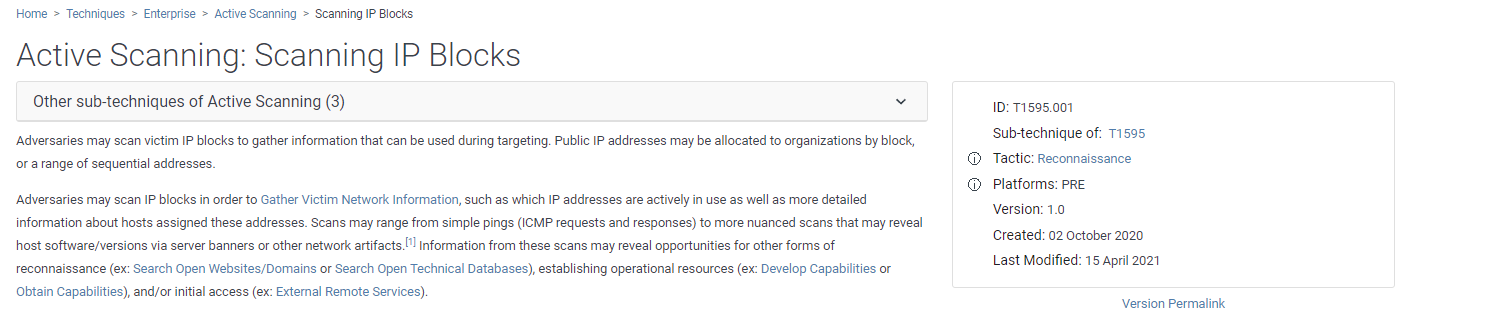
\includegraphics[width=1\linewidth]{imagenes/17.png}
    \caption{Información referente al procedimiento asignado \textit{Scanning \gls{IP}  Blocks} \cite{mitre_attack}}
    \label{fig:ejemplo-procedimiento}
\end{figure}

Adicionalmente, como se observa en la Figura \ref{fig:ejemplo-procedimiento-2}, se puede encontrar justo debajo ejemplos de técnicas de Detección y Mitigación, también identificadas bajo el criterio mencionado anteriormente.

\begin{figure}[H]
    \centering
    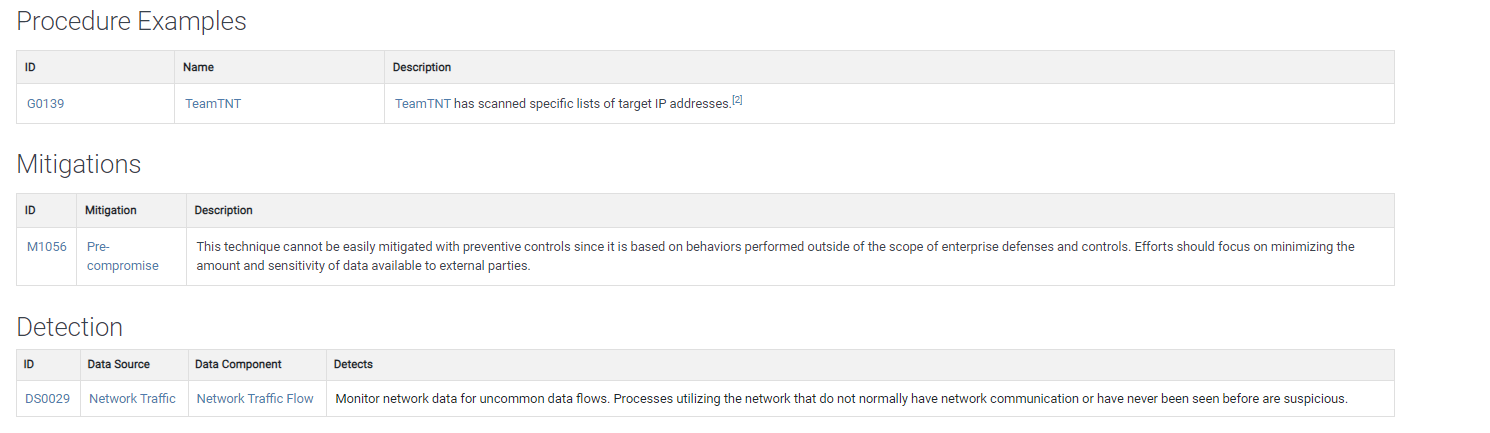
\includegraphics[width=1\linewidth]{imagenes/18.png}
    \caption{Ejemplos de mitigación y detección frente a \textit{Scanning \gls{IP} Blocks} \cite{mitre_attack}}
    \label{fig:ejemplo-procedimiento-2}
\end{figure}

\subsubsection{Frameworks basados en MITRE \gls{ATT&CK}}

Actualmente existen numerosos \textit{frameworks} basados en el marco adversario de MITRE para orquestar simulaciones de ataques en auditorías de seguridad tanto internas como externas. Algunos de estos \textit{frameworks} son:

\begin{itemize}
    \label{frameworks-mitre}
    \item \texttt{\gls{CALDERA}} \cite{caldera}: Desarrollado por el propio MITRE, este \textit{framework} permite planificar, ejecutar y evaluar campañas adversarias basadas en las técnicas definidas en la matriz de \gls{ATT&CK}. Con más de 800 artículos y libros publicados en plataformas académicas como Google Scholar y Scopus, puede considerarse el más utilizado en la actualidad y por tanto el elegido para la implementación de este proyecto, por lo que será explicado con mayor detalle en secciones posteriores.
    \vspace{0.5mm}
    \item \texttt{Red Team Automation (\gls{RTA})} \cite{rta}: Un conjunto de \textit{scripts} diseñados para generar tráfico malicioso que simula comportamientos específicos basados en MITRE \gls{ATT&CK}.  
    \vspace{0.5mm}
    \item \texttt{Atomic Red Team} \cite{atomic_red_team}: Es un conjunto de pruebas pequeñas y altamente portátiles, cada una diseñada para ejecutar una técnica única de MITRE \gls{ATT&CK}. Es útil para equipos de seguridad que desean probar sus defensas de manera incremental y sistemática.
    \vspace{0.5mm}
    \item \texttt{Infection Monkey} \cite{infection_monkey}: Una herramienta de seguridad de código abierto que simula ataques en la red para probar la resiliencia de los sistemas y la eficacia de las medidas de defensa en profundidad. Utiliza técnicas de MITRE \gls{ATT&CK} para evaluar cómo los adversarios podrían avanzar dentro de la red.
    \vspace{0.5mm}
    \item \texttt{Scythe} \cite{scythe}: Esta plataforma permite a los usuarios crear y ejecutar campañas de simulación de amenazas que replican el comportamiento de los adversarios basado en \gls{ATT&CK}.
\end{itemize}

\newpage

% ********************************************************************

\section{Modelos de IA para la detección de vectores de ataque}

Es innegable que en todos los campos tecnológicos se quiere aprovechar al máximo las novedades que está trayendo consigo la Inteligencia Artificial. Concretamente, en el sector de la ciberseguridad muchas empresas de desarrollo de software están tratando de acoplar el análisis e interpretación de datos masificados a través de modelos de \gls{ML} (\textit{Machine Learning}) y \gls{DL} (\textit{Deep Learning}) con el fin de agilizar diversas tareas que hasta la fecha han tenido que llevarse a cabo manualmente por personas, ocupando gran parte del horario laboral, y por tanto no pudiendo ser invertido en otras actividades en las que el desempeño humano es totalmente necesario para la toma de decisiones.

Es por ello que está incrementando considerablemente la cantidad de artículos científicos y de investigación publicados en los que se exploran distintas técnicas y se realizan pruebas haciendo uso de \textit{datasets} generados de forma natural o sintética.

Además de las propias empresas, es bien conocido que algunos grupos de cibercriminales o grupos de ciberterrorismo que operan a la escala de grandes empresas tienen sus propias áreas de \gls{I+D} (\textit{Investigation \& Development}) en las que investigan cómo a través de la IA \cite{barry2024} pueden refinar ataques a gran escala, generar \textit{phisings} sofisticados o \textit{malware} simplemente a través de la correcta redacción de un \textit{prompt} enviado a un \gls{LLM} que no está correctamente sanitizado o que incluso no tiene limitaciones éticas.

Existen distintos enfoques y técnicas para utilizar esta tecnología: Por un lado, el \textit{machine learning} permite resolver problemas concretos utilizando un volumen de datos más pequeño, pero solo aplica a problemas de dimensionalidad baja. Por el contrario, el \textit{deep learning} necesita más datos así como unos recursos de computación mayores (LeCun et. al \cite{LeCun2015}), pero puede utilizarse para cuestiones con un mayor nivel de abstracción.

Asimismo, la forma en la que estos modelos aprenden acerca de un problema difiere en función del nivel de etiquetado de los datos. Pueden distinguirse los siguientes tipos de aprendizaje:

\begin{itemize}
    \item \textit{Supervised Learning} (\gls{SL}): utiliza \textit{datasets} etiquetados y su finalidad es predecir un valor real (regresión) o bien un valor que esté contenido dentro de un conjunto (clasificación).

    \item \textit{Semi-Supervised Learning} (\gls{SSL}): el \textit{dataset} solo tiene algunas de sus partes etiquetadas, por lo que se extraen características relevantes y se representan los datos no etiquetados de forma que luego sea posible emplear el conocimiento adquirido en modelos de aprendizaje supervisado.

    \item \textit{Unsupervised Learning} (\gls{UL}): los datos no tienen que estar etiquetados, de modo que se trata de encontrar relación entre las diferentes instancias del conjunto de datos.

    \item \textit{Reinforcement Learning} (\gls{RL}): se basa en el ajuste de los parámetros para optimizar la llamada función de recompensa, la cual beneficiará al modelo al realizar una acción determinada.
\end{itemize}

Una técnica ampliamente utilizada en el aprendizaje no supervisado y semi-supervisado es el \textit{clustering}, que permite agrupar datos no etiquetados basándose en sus características y similitudes, como patrones inusuales o comportamientos similares que podrían indicar actividades maliciosas. Esta técnica se puede llevar a cabo utilizando distintos tipos de algoritmos, entre los más comunes se encuentran:

\begin{itemize}
    \item \textbf{K-means}: Es uno de los métodos más sencillos y populares. Funciona dividiendo el conjunto de datos en \( k \) grupos (\textit{clusters}) definidos por \( k \) centroides, que se ajustan iterativamente para minimizar la variación dentro de cada \textit{cluster}. A pesar de su simplicidad, K-means puede ser muy efectivo para detectar agrupaciones naturales en los datos.
    
    \item \textbf{\gls{DBSCAN}} (\textit{Density-Based Spatial clustering of Applications with Noise}): Es útil para identificar \textit{clusters} de cualquier forma y manejar ruido (datos atípicos). Agrupa puntos que están densamente conectados, es decir, puntos que están a una distancia mínima unos de otros. Esto permite encontrar estructuras complejas en los datos que K-means podría no detectar.

    \item \textbf{\gls{HC}} (\textit{Hierarchical clustering}): Este algoritmo crea una jerarquía de \textit{clusters}, que se puede representar mediante un dendrograma. 
    Existen dos enfoques principales: 
        \begin{itemize}
            \item  \textbf{\gls{AHC}} - Aglomerativo (\textit{bottom-up}), que comienza con puntos individuales y los fusiona en \textit{clusters} más grandes
            \item  \textbf{\gls{DHC}} Divisivo (\textit{top-down}), que empieza con todo el conjunto de datos y los divide en \textit{clusters} más pequeños.
        \end{itemize}
\end{itemize}

% ********************************

\subsection{Principales \textit{Datasets} de logs}

Al ser una gran fuente de información sensible, es altamente complejo encontrar \textit{datasets} de ficheros \textit{log} que no hayan sido generados de forma sintética. Del mismo modo, gran parte de los \textit{logfiles} de Linux utilizados como conjuntos de datos para \gls{IA} solo pueden ser accesibles pagando. 

Gracias a la contribución de Jieming Zhu et. al \cite{loghub2023}, se desarrolló un repositorio en \textit{GitHub} llamado LogHub, que contiene un gran conjunto de \textit{datasets} de logs de distintos ámbitos como sistemas distribuidos, supercomputadores, sistemas operativos, sistemas móviles, servicios y software.

\newpage

\begin{table}[H] 
\centering
\footnotesize
\begin{tabular}{|l|p{4cm}|c|c|c|}
\hline
\rowcolor{graylight}\texttt{Dataset} & \texttt{Descripción} & \texttt{Etiquetado} & \texttt{Duración} & \texttt{Nº Líneas} \\
\hline
\rowcolor{graylight}\multicolumn{5}{|c|}{\texttt{Sistemas Distribuidos}} \\
\hline
HDFS\_v1 & Logs del sistema de archivos distribuido Hadoop & Sí & 38.7 horas & 11,175,629 \\
\hline
HDFS\_v2 & Logs del sistema de archivos distribuido Hadoop & - & - & 71,118,073 \\
\hline
HDFS\_v3 & Log trazado instrumentado de HDFS (TraceBench) & Sí & - & 14,778,079 \\
\hline
Hadoop & Logs de trabajos de Hadoop MapReduce & Sí & - & 394,308 \\
\hline
Spark & Logs de trabajos de Spark & - & - & 33,236,604 \\
\hline
Zookeeper & Logs del servicio ZooKeeper & - & 26.7 días & 74,380 \\
\hline
OpenStack & Logs de infraestructura de OpenStack & Sí & - & 207,820 \\
\hline
\rowcolor{graylight}\multicolumn{5}{|c|}{\texttt{Supercomputadores}} \\
\hline
BGL & Logs del supercomputador  Blue Gene/L & Sí & 214.7 días & 4,747,963 \\
\hline
HPC & Logs de clúster de alto rendimiento & - & - & 433,489 \\
\hline
Thunderbird & Logs del supercomputador Thunderbird & Sí & 244 días & 211,212,192 \\
\hline
\rowcolor{graylight}\multicolumn{5}{|c|}{\texttt{Sistemas Operativos}} \\
\hline
Windows & Logs de eventos de Windows & - & 226.7 días & 114,608,388 \\
\hline
Linux & Logs de Linux & - & 263.9 días & 25,567 \\
\hline
Mac & Logs de Mac OS & - & 7.0 días & 117,283 \\
\hline
\rowcolor{graylight}\multicolumn{5}{|c|}{\texttt{Sistemas Móviles}} \\
\hline
Android\_v1 & Logs de framework de Android & - & - & 1,555,005 \\
\hline
Android\_v2 & Logs de framework de Android & - & - & 30,348,042 \\
\hline
HealthApp & Logs de aplicación de salud & - & 10.5 días & 253,395 \\
\hline
\rowcolor{graylight}\multicolumn{5}{|c|}{\texttt{Aplicaciones de Servidor}} \\
\hline
Apache & Logs de errores del servidor web Apache & - & 263.9 días & 56,481 \\
\hline
OpenSSH & Logs del servidor OpenSSH & - & 28.4 días & 655,146 \\
\hline
\rowcolor{graylight}\multicolumn{5}{|c|}{\texttt{Software Autónomo}} \\
\hline
Proxifier & Logs del software Proxifier & - & - & 21,329 \\
\hline
\end{tabular}
\caption{Conjunto de \textit{Datasets} de logs para el análisis impulsado por IA}
\label{tab:log_datasets}
\end{table}


Entre los anteriores, algunos de los más potentes son \gls{BGL} (\textit{Blue Gene/L}) y \gls{HDFS} (\textit{Hadoop Distributed File System}), que se han utilizado extensamente en investigaciones de detección de anomalías y fallos en sistemas de alta computación, debido a su gran variedad de eventos y la duración prolongada del registro de los \textit{logs} que contienen. 

Otro \textit{dataset} destacable a pesar de su menor volumen de datos, es el de Linux. Este puede ser generado con cierta facilidad ya que simplemente es necesario configurar un entorno en el cual utilizar la herramienta \textit{syslog} y automatizar el almacenamiento de distintos tipos de \textit{logs} dentro de un mismo fichero.


\subsubsection{3.3.1.1.  BGL} \label{BGL}

De las siglas "Blue Gene/L", \gls{BGL} es un \textit{dataset} que contiene \textit{logs} generados por el supercomputador \textit{Blue Gene/L}, desarrollado por IBM. Este \textit{dataset} se ha utilizado ampliamente en la investigación de técnicas de detección de anomalías y fallos en sistemas. Los \textit{logs} de \gls{BGL} incluyen una gran variedad de eventos de sistema, lo que permite a los probar diferentes enfoques de \gls{ML} y \gls{DL} para identificar patrones inusuales que podrían indicar un ataque o un fallo en el sistema.

\subsubsection{3.3.1.2.  HDFS} \label{HDFS}

El Hadoop Distributed File System (\gls{HDFS}) es otro \textit{dataset} significativo que consiste en \textit{logs} generados por sistemas distribuidos de \textit{Hadoop}. Este es útil para estudiar el comportamiento de sistemas de archivos distribuidos y detectar anomalías que podrían sugerir intentos de intrusión o errores en el sistema. Los \textit{logs} de \gls{HDFS} incluyen información detallada sobre operaciones de archivos, accesos y errores, proporcionando una rica fuente de datos para el entrenamiento y evaluación de modelos de detección de anomalías.

\subsubsection{3.3.1.3.  Linux\_2k} \label{Linux_2k}

El \textit{dataset} Linux\_2k es una colección de \textit{logs} generados por sistemas Linux, específicamente recolectados desde el archivo \textit{/var/log/messages} en un servidor Linux durante un período de más de 260 días, como parte del proyecto \textit{Public Security Log Sharing Site} liderado por el Dr. Anton Chuvakin \cite{chuvakin2010public}. Este sitio proporciona una variedad de muestras de logs gratuitas de diferentes sistemas, dispositivos de seguridad y red, aplicaciones, etc., recolectados de sistemas reales y que en muchos casos contienen evidencias de compromisos y otras actividades maliciosas. \\

El proyecto, iniciado el 23 de junio de 2009 y actualizado el 11 de agosto de 2010, busca ofrecer \textit{logs} sin sanitización ni anonimización, permitiendo así un análisis genuino de los datos tal y como fueron registrados por los sistemas de \textit{logging}, lo que lo convierte en un \textit{dataset} especialmente valioso para este proyecto de investigación.

\newpage

% ********************************************************************

\section[SIEM]{Sistemas de Gestión de Información y Eventos de Seguridad (SIEM)}

Actualmente existen distintos tipos de software de seguridad orientados a la prevención, detección y respuesta a cualquier tipo de incidentes de seguridad. Estos trabajan, por lo general, con cantidades ingentes de datos, por lo que están diseñadas de forma óptima para minimizar tiempos de espera. 

Sin embargo, a pesar de la funcionalidad que ofrecen, estos presentan un cuello de botella con respecto a la toma de determinadas decisiones. A día de hoy es necesario en muchos casos que un profesional determine manualmente si hay algún tipo de intento de intrusión maliciosa, si hay un falso positivo o si simplemente no hay actividad inusual.

Está claro que es necesaria la intervención humana, pero el hecho de automatizar algunas tareas puede propulsar la inversión de ese tiempo de esfuerzo en otras actividades de mayor interés. Por este hecho, surgen distintas herramientas (Figura \ref{tab:herramientas_independientes}) de seguridad que llevan a cabo este proceso:

\vspace{0.2cm}

\begin{table}[h]
    \centering
    \footnotesize
    \begin{tabular}{|l|p{10cm}|}
        \hline
        \rowcolor{graylight}\texttt{Nombre} & \texttt{Descripción} \\
        \hline
        \gls{SIEM} & Gestión de eventos e información de seguridad. \\
        \hline
        Firewall & Control de tráfico de red. \\
        \hline
        \gls{WAF} & Firewall de aplicaciones web. \\
        \hline
        \gls{EDR} & Monitorización y respuesta en \textit{endpoints}\footnotemark.  \\
        \hline
        Antivirus & Protección frente a software malicioso. \\
        \hline
        Antimalware & Protección avanzada contra malware. \\
        \hline
    \end{tabular}
    \caption{Herramientas software de seguridad}
    \label{tab:herramientas_independientes}
\end{table}

\footnotetext{\ Dispositivo final que proporciona un punto de entrada en un activo, como un dispositivo conectado a red o un servicio web.}

De los anteriores, uno de los más completos y utilizados es el \gls{SIEM} \cite{siemibm2024}, ya que puede integrar las funcionalidades de distintas herramientas software de seguridad (Figura \ref{tab:integrables_siem}). Inicialmente eran dos herramientas distintas: \gls{SIM} (\textit{Security Information Management}) y \gls{SEM} (\textit{Security Events Management}) pero a partir de 2005 se hizo mención por primera vez como una herramienta conjunta por \textit{Williams y Nicolett} \cite{williams2005improve}. Son principalmente utilizados en los \gls{SOC} para supervisar y monitorizar la actividad para poder detectar ataques y mitigarlos eficientemente. 

\begin{table}[h]
    \centering
    \footnotesize
    \begin{tabular}{|l|p{10cm}|}
        \hline
        \rowcolor{graylight}\texttt{Nombre} & \texttt{Descripción} \\
        \hline
        \gls{SOAR} & Orquestación, automatización y respuesta. \\
        \hline
        \gls{IDS} & Sistemas de detección de intrusiones. \\
        \hline
        \gls{NIDS} & Detección de intrusiones en la red. \\
        \hline
        \gls{HIDS} & Detección de intrusiones en \textit{hosts}. \\
        \hline
        \gls{IPS} & Sistemas de prevención de intrusiones. \\
        \hline
        \gls{IRS} & Sistemas de respuesta de intrusiones. \\
        \hline
    \end{tabular}
    \caption{Herramientas integrables o complementarias al SIEM}
    \label{tab:integrables_siem}
\end{table}

\newpage

Tal y como define González-Granadillo et al. \cite{s21144759}, los \gls{SIEM} han sido desarrollados en respuesta para ayudar a los administradores a diseñar políticas de seguridad y gestionar eventos de diferentes fuentes. Generalmente, están compuestos de bloques separados (por ejemplo, dispositivo fuente, recolección de registros, normalización de análisis, motor de reglas, almacenamiento de registros, monitoreo de eventos) que pueden trabajar independientemente entre sí, pero sin su coordinación, el \gls{SIEM} no funcionaría adecuadamente. \\

Las dos principales métricas utilizadas \cite{plextrac2024} para medir su funcionamiento son el tiempo medio hasta la detección (\gls{MTTD}) y el tiempo medio hasta la respuesta (\gls{MTTR}).

\begin{equation}
\text{\gls{MTTD}} = \frac{\text{\textit{Total Sum of Detection time} (\gls{TSD})}}{\text{\textit{Total Number of Incidents} (\gls{TNI})}}
\end{equation}

Donde \gls{TSD} es la suma total del tiempo acumulado que ha pasado desde el inicio de los incidentes hasta su descubrimiento, y la \gls{TNI} es el número total de incidentes detectados.

\begin{equation}
\text{\gls{MTTR}} = \frac{\text{\textit{Total Sum of Detection to Remediation time} (\gls{TSDR})}}{\text{\textit{Total Number of Incidents Remediated} (\gls{TNIR})}}
\end{equation}

Donde \gls{TSDR} es el tiempo acumulado que ha pasado desde que se descubrieron los incidentes hasta su remediación, y la \gls{TNIR} es el número total de incidentes remediados.

%%%%%%%%%%%%%%%
 

\subsection{Principales SIEM en el escenario actual}

En la actualidad, existen \gls{SIEM} de pago y también alternativas \textit{opensource}. La principal diferencia reside, además del precio, en la personalización y el soporte técnico. Las soluciones de pago generalmente ofrecen una mayor integración con otros productos y un soporte técnico más completo y directo por parte de los proveedores, como actualizaciones automáticas, asistencia para la configuración y solución rápida de problemas.

Por otro lado, las alternativas \textit{opensource} como las mencionadas por Ángel Veloy et. al \cite{veloy2019ventajas}, si bien pueden ser menos costosas, a menudo requieren un mayor conocimiento técnico para su implementación y mantenimiento, y el soporte suele depender de la comunidad de usuarios, lo cual puede no ser tan inmediato o accesible. 

Además, estas pueden tener menos características \textit{out-of-the-box} comparadas con las versiones de pago, lo que podría requerir más desarrollo personalizado para integrarlas completamente en entornos empresariales complejos.

Es posible clasificar los principales \gls{SIEM} a través del Cuadrante Mágico de Gartner \cite{GartnerSIEM2024}, un una herramienta analítica que clasifica a los proveedores en un mercado tecnológico específico en cuatro categorías: Líderes, Visionarios, Desafiantes y Jugadores de Nicho.

\begin{table}[h]
    \centering
    \footnotesize
    \begin{tabularx}{\textwidth}{|>{\hsize=0.8\hsize\RaggedRight\arraybackslash}X|>{\hsize=1.2\hsize\RaggedRight\arraybackslash}X|>{\Centering\arraybackslash}c|>{\hsize=1\hsize\RaggedRight\arraybackslash}X|}
        \hline
        \rowcolor{graylight}\texttt{\gls{SIEM}} & \texttt{Empresa} & \texttt{\gls{OSS}} & \texttt{Categoría Gartner} \\
        \hline
        Splunk Enterprise Security & Splunk Inc. & No & Líder \\
        \hline
        \gls{IBM} QRadar & \gls{IBM} & No & Líder \\
        \hline
        LogRhythm NextGen SIEM Platform & LogRhythm, Inc. & No & Líder \\
        \hline
        ArcSight \gls{ESM} & Micro Focus & No & Desafiante \\
        \hline
        AlienVault \gls{OSSIM} & AT\&T Cybersecurity & Sí & Jugador de Nicho \\
        \hline
        \gls{ELK} Stack (Elasticsearch, Logstash, Kibana) & Elastic & Sí & Visionario \\
        \hline
        Wazuh & Wazuh, Inc. & Sí & Jugador de Nicho \\
        \hline
        Graylog & Graylog, Inc. & Sí & Jugador de Nicho \\
        \hline
    \end{tabularx}
    \caption{Principales SIEM en escenario actual según Cuadrante Mágico de Gartner \cite{GartnerSIEM2024}}
    \label{tab:siem_gartner}
\end{table}

Los precios de los \gls{SIEM} de pago como Splunk, perteneciente a CISCO \cite{cisco},  o \gls{IBM} varían según el volumen de datos y la capacidad de cómputo que necesita utilizarse. De ello surgen varios modelos. \\

\textbf{Modelo basado en el volumen de datos de Ingesta diaria}

Calcula el coste basado en la cantidad de datos procesados diariamente: 

\vspace{-0.3cm}

\begin{equation}
    C_{\text{datos}} = V_{\text{GB}} \times P_{\text{GB}}
\end{equation}

Donde
\begin{itemize}
    \item $C_{\text{datos}}$ es el coste total basado en el volumen de datos.
    \item $V_{\text{GB}}$ es el volumen de datos en gigabytes por día.
    \item $P_{\text{GB}}$ es el precio por gigabyte por día.
\end{itemize}

\vspace{0.3cm}

\textbf{Modelo basado en unidades de cómputo virtual (SVC)} \footnotemark

Determina el coste a partir del nº de unidades de cómputo virtual asignadas:

\begin{equation}
    C_{\text{SVC}} = N_{\text{SVC}} \times P_{\text{SVC}}
\end{equation}

\vspace{-0.2cm}

Donde:
\begin{itemize}
    \item $C_{\text{SVC}}$ es el coste total basado en las unidades de cómputo.
    \item $N_{\text{SVC}}$ es el número de unidades de cómputo virtual de Splunk.
    \item $P_{\text{SVC}}$ es el precio por unidad de cómputo.
\end{itemize}

\footnotetext{\  Específicamente utilizado por Splunk Enterprise Security de Splunk Inc \cite{splunk2024}.}

\newpage

\subsection{Nuevas tendencias y mejoras en \gls{SIEM}}

Los \gls{SIEM} son, como se comenta anteriormente, un pilar fundamental en el modelo de infraestructura de ciberseguridad actual, no solo por su capacidad de centralizar y sintetizar datos, sino también por su evolución constante en la integración con tecnologías emergentes. 

Según González-Granadillo et al. \cite{s21144759}, estos están convergiendo gradualmente con herramientas de análisis de \textit{big data}, lo que amplía su capacidad para manejar y analizar un volumen más extenso de datos en tiempo real. Esta convergencia permite a los \gls{SIEM}s detectar patrones complejos de comportamiento que podrían indicar la presencia de amenazas sofisticadas.

Sin embargo, es crucial adaptarse a la \gls{GDPR}. Por ello, los proveedores de \gls{SIEM} están mejorando sus plataformas para ofrecer mayores capacidades de anonimización y gestión de la privacidad. Esto incluye funciones que permiten a las organizaciones cumplir con los derechos de acceso, rectificación, limitación del procesamiento, y supresión de datos personales esta garantiza a los individuos \cite{EU_GDPR_2016}. 

Además, algunas soluciones \gls{SIEM} modernas incorporan módulos específicos diseñados para gestionar el cumplimiento de la \gls{GDPR}, facilitando así la auditoría y generación de informes necesarios para demostrar el cumplimiento a los reguladores. Por este motivo, resulta realmente complejo encontrar \textit{datasets raw} de eventos de seguridad que sean públicos o que no hayan pasado previamente por algún tipo de proceso de anonimización antes de haber sido liberados. \\

\vspace{4mm}
\noindent\rule[-1ex]{\textwidth}{0.5pt}\\
\vspace{4mm}

En base al estudio llevado a cabo de todas las tecnologías anteriores, se establecen las siguientes conclusiones:

Se llevará a cabo la simulación de ataques mediante el \textit{framework} \gls{CALDERA} dentro del marco táctico de MITRE \gls{ATT&CK} y se preprocesarán los \textit{logs} obtenidos con el fin de generar un \textit{dataset}, extrayendo las características principales que permitan realizar dicha clasificación. A continuación se realizará un estudio de dicho \textit{dataset} y otros diferentes que hayan sido preprocesados de manera equivalente. Seguidamente, se aplicarán técnicas de \gls{ML}, más concretamente algoritmos de \textit{clustering} combinados con distintas técnicas de extracción de características y de reducción de la dimensionalidad, para la detección de patrones de ataque. Por último se llevará a cabo un análisis de los resultados obtenidos mediante distintas métricas de evaluación y se efectuará una comparativa con otros proyectos similares, así como un esbozo de cómo puede integrarse esta tecnología en los \gls{SIEM} actuales.


\chapter{Metodología de trabajo}

En este capítulo se profundizará en el dominio del problema que se quiere resolver, examinando la metodología a seguir para poder llevar a cabo este proceso, así como las tecnologías y herramientas que se utilizarán para que sea posible su desarrollo.

% ********************************************************************

\section{Complejidad del problema a resolver}

La principal complejidad que presenta el análisis de \textit{logs} es, sin duda, la gran heterogeneidad que tiene su representación, así como la estructura abstracta de algunos de sus campos. En el caso de Linux, esta abstracción viene dada por el campo \textit{message}, probablemente el más importante, ya que este contiene la descripción del evento registrado.

\vspace{-1mm}

\begin{figure}[H]
    \centering
    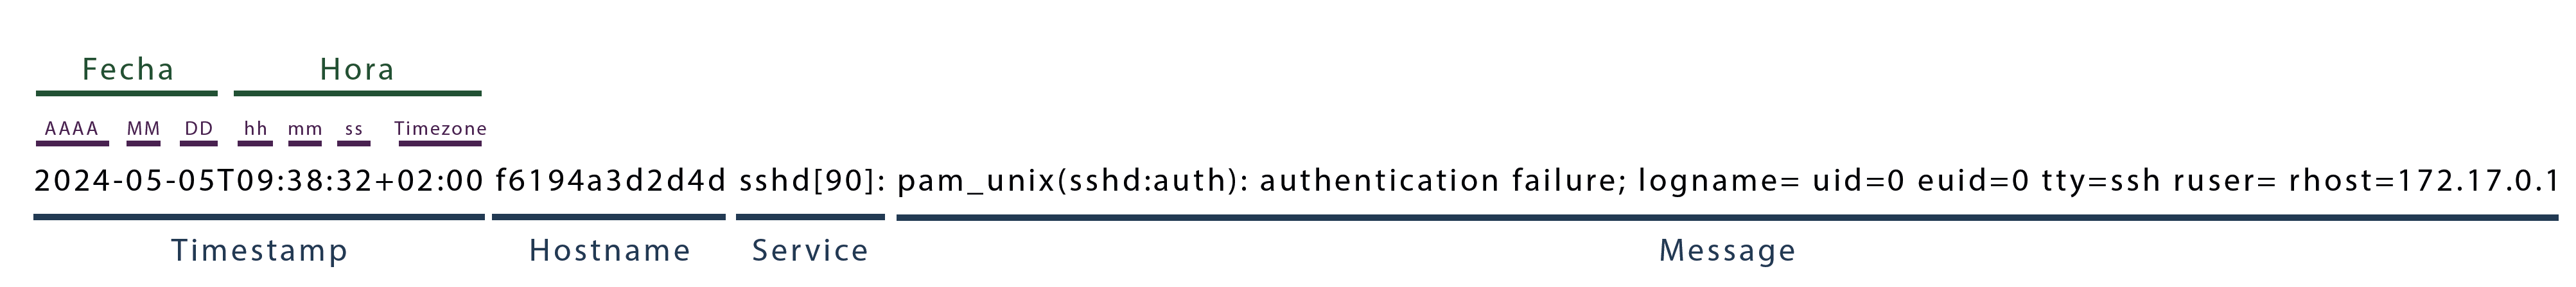
\includegraphics[width=1\linewidth]{imagenes/linux-log-structure.png}
    \caption{Sintaxis de un \textit{log} de Linux}
    \label{fig:linux-log-structure}
\end{figure}

\vspace{-0.5mm}

Como se puede observar en la Figura \ref{fig:linux-log-structure}, los \textit{logs} de Linux presentan un total de 4 campos: \textit{timestamp}, \textit{hostname}, \textit{service} y \textit{message}. Este último representa un claro aumento en la complejidad de preprocesamiento ya que no sigue un patrón concreto sino que esta elección se delega al servicio que está sirviendo la información, como ocurre en la Figura \ref{fig:linux-log-structure-message}.

\vspace{-0.5mm}

\begin{figure}[H]
    \centering
    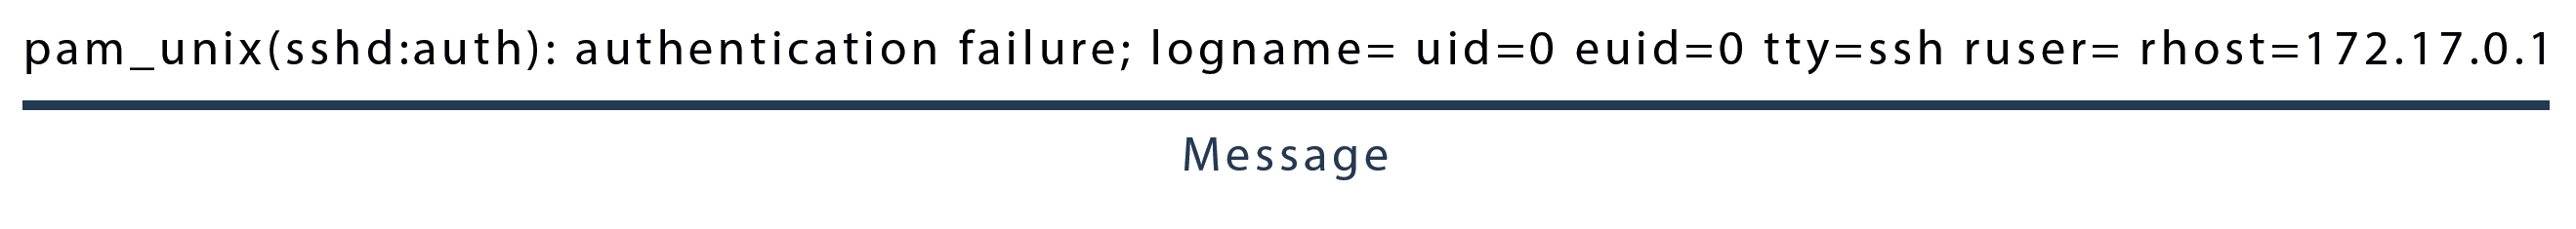
\includegraphics[width=1\linewidth]{imagenes/linux-log-structure-message.png}
    \caption{Sintaxis del \textit{message} de un \textit{log} de Linux}
    \label{fig:linux-log-structure-message}
\end{figure}

Dentro del mismo puede extraerse otra información útil; en el ejemplo proporcionado se informa de un fallo en la autenticación, así como la \gls{tty} utilizada, la \gls{IP} del host remoto involucrado o el identificador de usuario asociado.

Por otro lado, la sintaxis del \textit{timestamp} sigue el formato \gls{ISO} 8601 \cite{iso8601}, el cual consta de la estructura representada en la Figura \ref{fig:linux-log-structure-timestamp}. Analizando los elementos por lo que se compone, se extrae la siguiente información:

\begin{table}[H]
\centering
\footnotesize
\begin{tabularx}{\textwidth}{|>{\raggedright\arraybackslash}p{3cm}|>{\raggedright\arraybackslash}X|}
\hline
\rowcolor{graylight}\texttt{Campo} & \texttt{Descripción} \\
\hline
Fecha & La parte de la fecha está representada en el formato \texttt{YYYY-MM-DD}, donde:
\begin{itemize}
    \item \texttt{YYYY} representa el año en cuatro dígitos.
    \item \texttt{MM} representa el mes en dos dígitos (01 a 12).
    \item \texttt{DD} representa el día del mes en dos dígitos (01 a 31).
\end{itemize} \\
\hline
Hora & La parte de la hora sigue el formato \texttt{hh:mm:ss}, donde:
\begin{itemize}
    \item \texttt{hh} representa la hora en formato de 24 horas (00 a 23).
    \item \texttt{mm} representa los minutos (00 a 59).
    \item \texttt{ss} representa los segundos (00 a 59).
\end{itemize} \\
\hline
Separador & La letra \texttt{T} se utiliza como delimitador entre la fecha y la hora, indicando que la información que sigue es la hora correspondiente a la fecha especificada previamente. \\
\hline
Zona horaria & La parte final del \textit{timestamp} indica la diferencia con respecto al Tiempo Universal Coordinado (\gls{UTC}), expresada en el formato \texttt{±hh:mm}. Por ejemplo, \texttt{+02:00} indica que la hora está dos horas adelantada con respecto a \gls{UTC}. \\
\hline
\end{tabularx}
\caption{Descripción del formato de \textit{timestamp} según el estándar ISO 8601 \cite{iso8601}}
\label{tab:timestamp-format}
\end{table}

\begin{figure}[H]
    \centering
    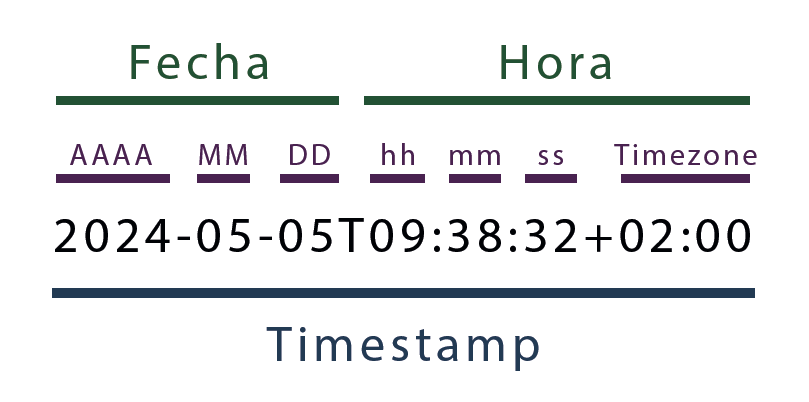
\includegraphics[width=0.6\linewidth]{imagenes/linux-log-structure-timestamp.png}
    \caption{Estructura del \textit{timestamp} de un \textit{log} de Linux}
    \label{fig:linux-log-structure-timestamp}
\end{figure}

Para este proyecto, se hará uso de otros \textit{datasets} de \textit{logs} que contienen una sintaxis que difiere bastante con la ofrecida por \textit{syslog}, por lo que será necesario llevar a cabo un pre-procesamiento de todos los tipos de eventos para que sean homogéneos, de modo que el modelo pueda interpretarlos de forma correcta. \\

En el caso de \gls{BGL}, como se puede observar en la Figura \ref{fig:bgl-log-structure}, existen nueve campos, aunque algunos de ellos redundantes: \textit{timestamp (epoch-time)}, \textit{date}, \textit{service}, \textit{detailed-timestamp}, \textit{hostname}, \textit{compontent}, \textit{severity}, \textit{type} y \textit{message}. De aquí se puede extraer que se repiten los cuatro campos de los \textit{logs} de Linux, y se añaden otros que pueden resultar muy útiles: la severidad y el tipo de evento.

\begin{figure}[H]
    \centering
    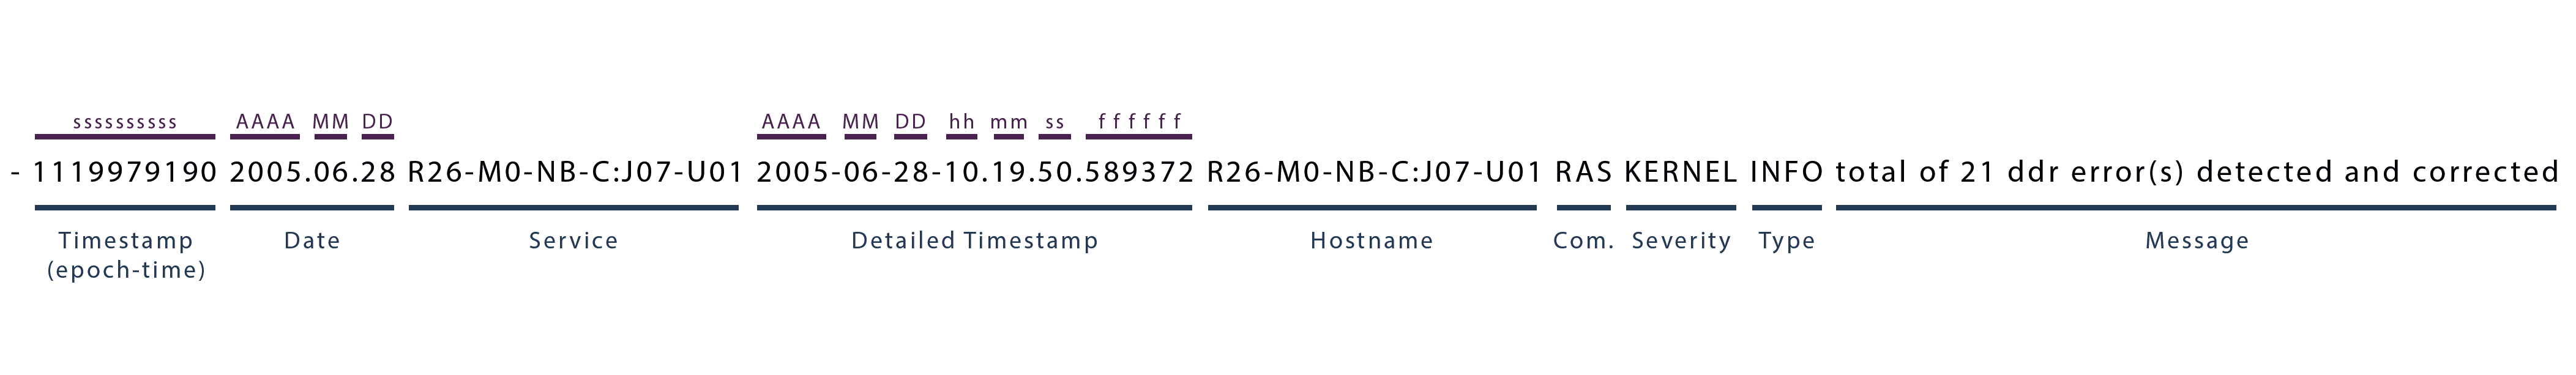
\includegraphics[width=1\linewidth]{imagenes/bgl-log-structure.png}
    \caption{Sintaxis de un \textit{log} de \gls{BGL}}
    \label{fig:bgl-log-structure}
\end{figure}

Otro factor a tener en cuenta es que cambia la estructura del \textit{timestamp}, analizando la Figura \ref{fig:bgl-log-timestamp}, se observa que los delimitadores son guiones y puntos, y que también contiene un campo extra asociado a una mayor precisión en el momento de captura del evento, ya que también mide a nivel de microsegundos, pero se pierde la precisión de la zona horaria.

\vspace{-1mm}

\begin{figure}[H]
    \centering
    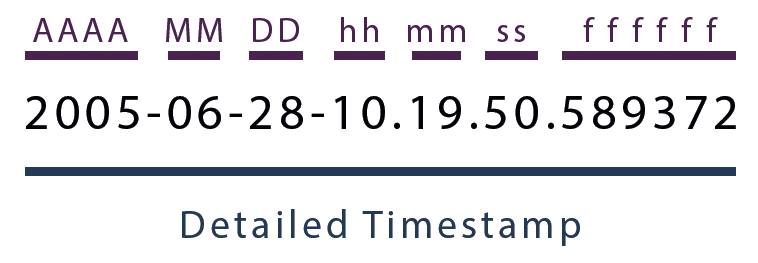
\includegraphics[width=0.6\linewidth]{imagenes/bgl-log-structure-timestamp.png}
    \caption{Estructura del \textit{timestamp} de un \textit{log} de \gls{BGL}}
    \label{fig:bgl-log-timestamp}
\end{figure}

Por último, en el caso de \gls{HDFS}, según se ilustra en la Figura \ref{fig:hdfs-log-structure} los eventos se organizan en cuatro campos: \textit{timestamp}, \textit{thread ID}, \textit{type} y \textit{message}. El único campo nuevo es el identificador de la hebra, aunque no es relevante para el estudio que se está llevando a cabo.

\vspace{-1mm}

\begin{figure}[H]
    \centering
    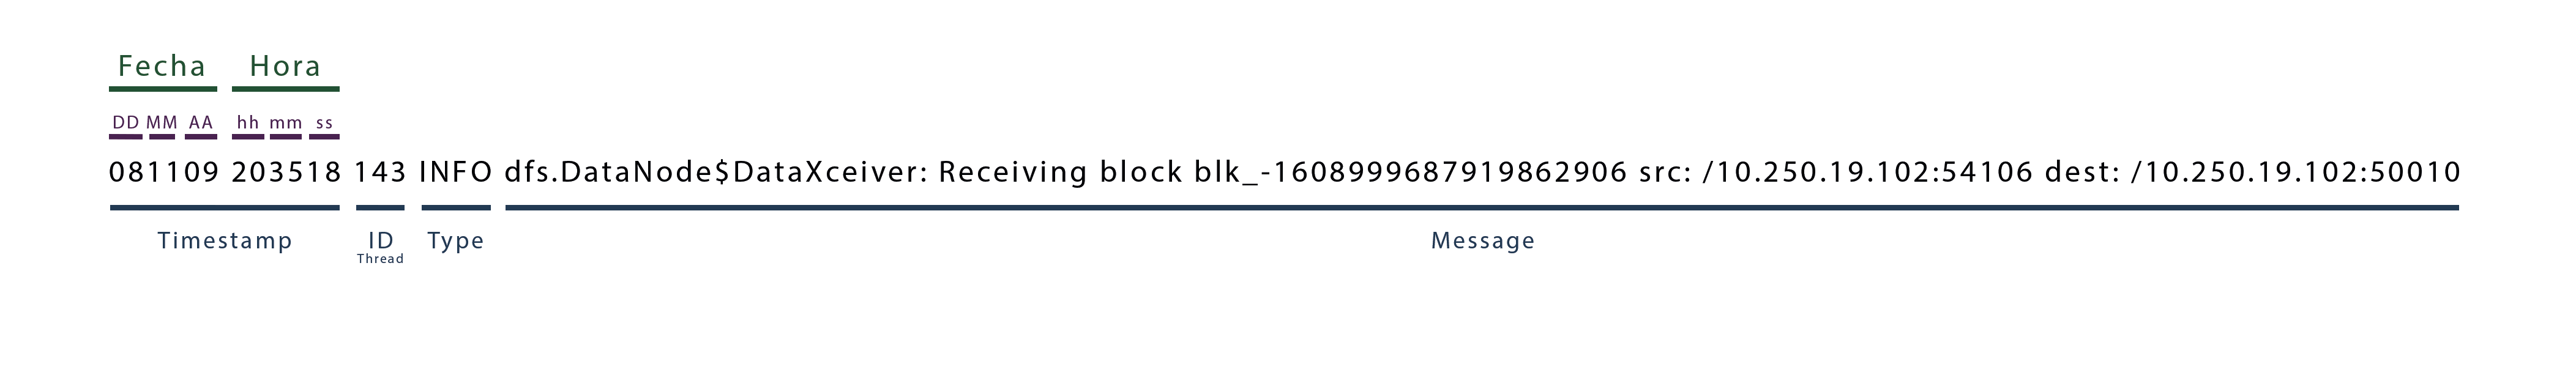
\includegraphics[width=1\linewidth]{imagenes/hdfs-log-structure.png}
    \caption{Sintaxis de un \textit{log} de \gls{HDFS}}
    \label{fig:hdfs-log-structure}
\end{figure}

También varía cómo se organiza el campo de \textit{timestamp}. Según se ve en la Figura \ref{fig:hdfs-log-structure-timestamp}, este es menos preciso en comparación con los anteriores, pero sigue siendo útil para llevar a cabo el estudio. Además, también se mantiene el campo \textit{message} con una estructura irregular.

\vspace{-1mm}

\begin{figure}[H]
    \centering
    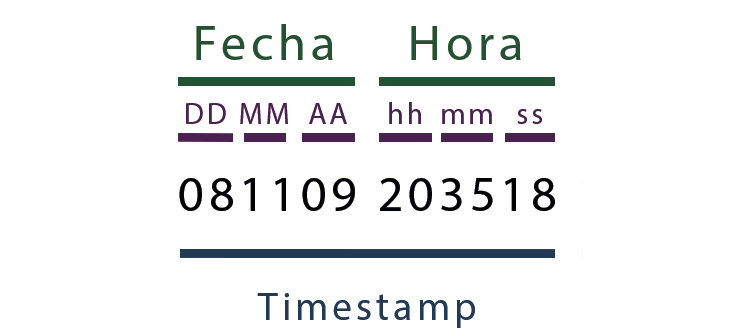
\includegraphics[width=0.6\linewidth]{imagenes/hdfs-log-structure-timestamp.png}
    \caption{Estructura del \textit{timestamp} de un \textit{log} de \gls{HDFS}}
    \label{fig:hdfs-log-structure-timestamp}
\end{figure}

Normalmente, todos los \textit{logs} de servicios software, dispositivos y otros sistemas operativos contienen los mismos campos. De hecho, para que un producto de este tipo pueda pasar una evaluación del tipo \gls{CC} (\textit{Common Criteria}) (reconocida a nivel mundial), es necesario que los registros de \textit{logs} cumplan con el \gls{SFR} \textit{FAU\_GEN.1}  \cite{commoncriteria}, el cual especifica el contenido mínimo que debe tener un evento registrado. \\

En conclusión, puede diferirse que los \textit{datasets} de eventos son de tipo no estructurado, por lo que pueden llevarse a cabo varios enfoques. Para este trabajo se hará un acercamiento mediante diferentes métodos de \textit{clustering} para poder detectar vectores de ataque y llevar a cabo agrupaciones de \textit{logs} para su posterior análisis. Previamente será necesario el preprocesado de los datos para unificar su formato, extrayendo más características importantes del campo \textit{message} junto con aquellas anteriormente mencionadas a través del uso de técnicas de \textit{parsing}.

\vspace{5mm}

% ********************************************************************

\section{Algoritmos de \textit{machine learning} escogidos}

Existen diversos métodos que abordan la clasificación y agrupamiento de \textit{logs} para poder detectar posibles patrones de ataque en sistemas Linux. Este Trabajo se centrará principalmente en el \textit{clustering} \cite{Aggarwal2013}. 

En primer lugar es necesario establecer una definición para esta técnica; en base a la proporcionada por \textit{Barreno Recio} et. al \cite{BarrenoRecio2023}.  \\

\begin{definition}
\shorthrule \vspace{0.1cm}
\\
El \textit{clustering} \label{clustering} se refiere al método de agrupación no supervisada de un conjunto de datos \(D = \{F_1, F_2, \ldots, F_n\}\) en \(k\) grupos \(C = \{C_1, C_2, \ldots, C_k\}\) utilizando una métrica de similitud diseñada para maximizar la homogeneidad entre los elementos de un mismo grupo y aumentar la heterogeneidad con respecto a los elementos de los otros grupos.
\\ \vspace{0.1cm}
\fullhrule
\end{definition}


De tal modo, la idea consiste en poder agrupar conjuntos de \textit{logs} que tengan características similares, de modo que entre dichas agrupaciones se encuentren vectores de ataque distintos como \gls{DoS} o fuerza bruta a servicios, como es el caso de la Figura \ref{fig:SSH-bruteforce-example}. Normalmente cuando se producen este tipo de ataques se genera una secuencia significativamente grande de eventos prácticamente equivalentes entre sí.

\begin{figure}[H]
    \centering
    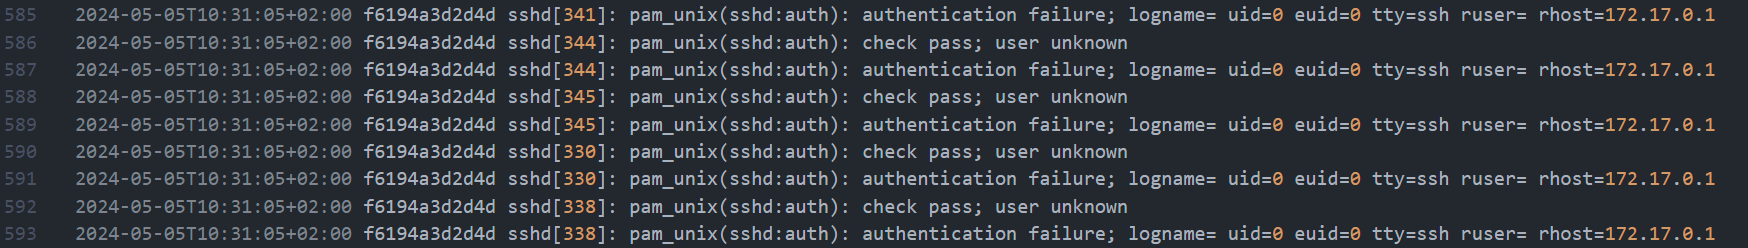
\includegraphics[width=1\linewidth]{imagenes/ssh-bruteforce-example.png}
    \caption{Ejemplo de secuencia de \textit{logs} generados por fuerza bruta a \gls{SSH}}
    \label{fig:SSH-bruteforce-example}
\end{figure}

Por tanto, basándonos en la definición anterior, el conjunto de datos D será un fichero que contenga una secuencia de eventos y estos serán agrupados en \textit{k} grupos de tipos de eventos distintos.

\newpage

\subsubsection*{Factores de un modelo de \textit{clustering}}

\setlist[itemize]{noitemsep, topsep=0pt}

\begin{table}[H]
\centering
\footnotesize
\renewcommand{\arraystretch}{0.9} 
\begin{tabularx}{\textwidth}{|>{\raggedright\arraybackslash}p{2.25cm}|>{\raggedright\arraybackslash}X|}
\hline
\rowcolor{graylight}\texttt{Factor} & \texttt{Descripción} \\
\hline
Representación de los datos & 
\begin{itemize}
    \item Adaptados: los datos son transformados para mejorar la estructura del modelo.
    \item No adaptados: los datos son utilizados en su forma original.
\end{itemize} \\
\hline
Medida de similitud & 
\begin{itemize}
    \item Tiempo: considerando las variaciones temporales.
    \item Cambio: observando las diferencias entre estados.
    \item Forma: evaluando la estructura de los datos.
\end{itemize} \\
\hline
Algoritmo de \textit{clustering} & 
\begin{itemize}
    \item Particional: K-Means, Fuzzy C-Means
    \item Jerárquico: \gls{AHC}, \gls{DHC}, \gls{HDBSCAN}, \gls{BIRCH}, \gls{FINCH}
    \item Densidad: \gls{DBSCAN}, \gls{OPTICS}, \gls{DENCLUE}, \gls{SNN}, \gls{DenMune}
    \item Cuadrícula: \gls{STING}, \gls{CLIQUE} 
\end{itemize} \\
\hline
Medidas de Evaluación &
\begin{itemize}
    \item Interna: \gls{KFCV}, \gls{LOOCV}
    \item Externa: uso de otros \textit{datasets} distintos al usado para el entrenamiento como \gls{HDFS}, \gls{BGL} o Linux\_2k.
\end{itemize} \\
\hline
\end{tabularx}
\caption{Factores de un modelo de \textit{clustering}}
\label{tab:clustering-factors}
\end{table}

\subsubsection*{Tipos de agrupamiento en técnicas de \textit{clustering}}

Además de los distintos factores indicados en la Tabla \ref{tab:clustering-factors}, se puede distinguir entre dos tipos de agrupamiento para el \textit{clustering}: el primero de ellos es el compacto, en el cual los elementos del grupo son muy parecidos y se representan a través de su punto central, mientras que el segundo es el agrupamiento encadenado \cite{https://doi.org/10.1002/widm.30}, en el cual un elemento de un grupo es más similar a otro de los elementos del grupo que los demás, produciéndose un efecto de cadena entre los elementos a través de una especie de ruta. Se puede ver en más detalle en la Figura \ref{fig:agrupamiento-clustering}.

\begin{figure}[H]
    \centering
    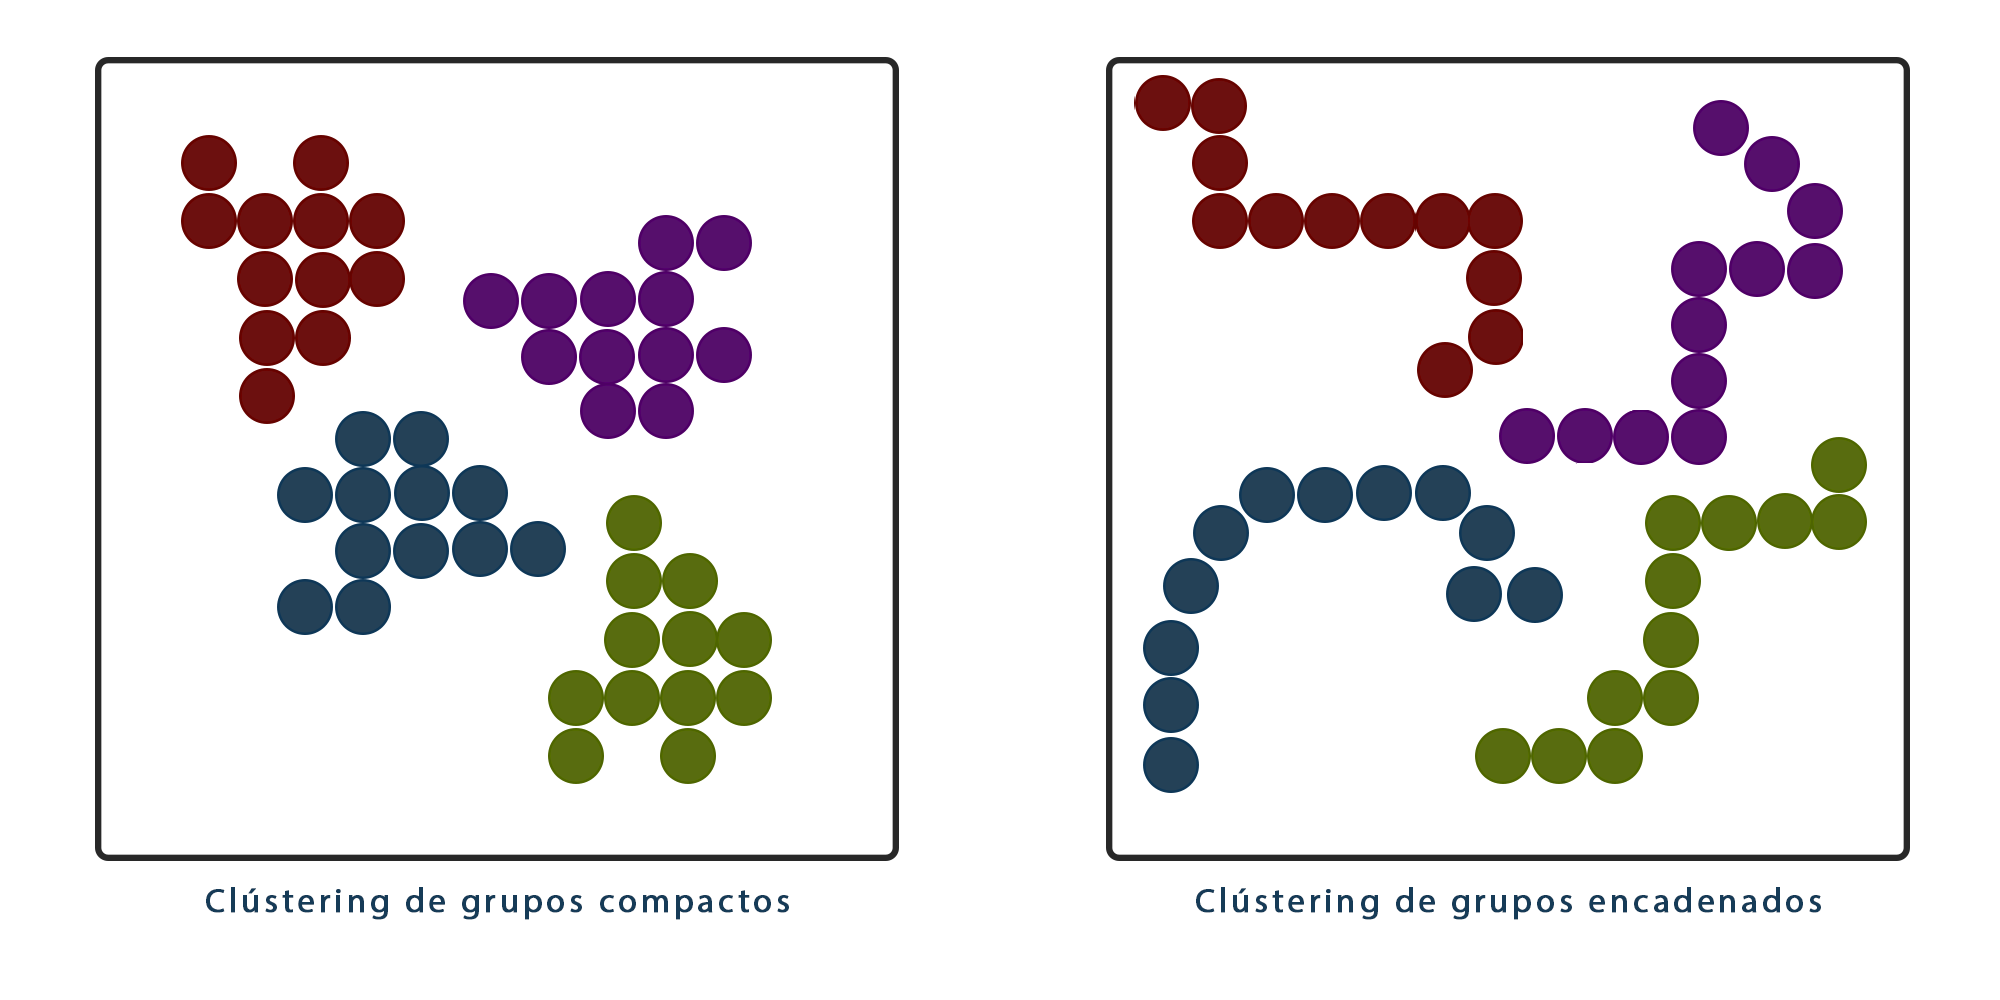
\includegraphics[width=0.75\linewidth]{imagenes/tipos-grupos-clustering.png}
    \caption{Tipos de agrupamiento en técnicas de \textit{clustering}} 
    \label{fig:agrupamiento-clustering}
\end{figure}

\newpage

\subsection{K-means}
\label{k-means}
Se trata de un algoritmo de \textit{clustering} basado en partición, es decir, este divide los datos en \textit{k} grupos de forma que cada grupo está compuesto por, al menos, un elemento. La forma de generar estos grupos consiste en tomar una serie de elementos que sean representativos, también conocidos como prototipos. 

La dificultad principalmente reside en escoger estos elementos representativos de manera que la partición sea lo más óptima posible. Para ello se lleva a cabo un proceso de iteración dividido en dos pasos:
\begin{itemize}
    \item Asignación: a partir de los prototipos iniciales se asignan los elementos al \textit{cluster} del prototipo que esté a menor distancia.
    \item Optimización: se vuelve a repetir el mismo proceso hasta que se cumpla una condición establecida, como un máximo de iteraciones o un error.
\end{itemize}

\vspace{-3mm}

\subsubsection*{Pseudocódigo del algoritmo K-means}

\vspace{-2mm}

\begin{myalgorithm}[H]
\footnotesize
\caption{K-means}
\textbf{Datos:} \textbf{D} Agrupación de datos a amontonar, \textbf{k} número de clúster\\
\textbf{Resultado:} Total de datos que forman \textit{D} agrupados en uno de los \textit{k} clúster
\begin{algorithmic}[1]
\State \textbf{Inicio;}
\State \textit{centroides} = lista de \textit{k} elementos aleatorios no repetidos de \textit{D};
\State \textit{clusters} = lista de \textit{k} clúster;
\Repeat
    \For{\textit{cada punto} $P$ \textbf{de} \textit{D}}
        \State \textit{centroideMasCercano} = centroides[0];
        \For{$c$ \textbf{en} \textit{centroides}}
            \If{$dist(P,c) < dist(P,centroideMasCercano)$}
                \State centroideMasCercano = $c$;
            \EndIf
        \EndFor
        \State Asignar $P$ al clúster al que pertenece centroideMasCercano;
    \EndFor
    \For{\textit{clust} \textbf{en} \textit{clusters}}
        \State Calcular Promedio del \textit{clust};
        \State Actualizar \textit{centroide};
    \EndFor
\Until{\textit{se cumplan un número de iteraciones, que todos los grupos cumplan una determinada tolerancia, que los grupos no cambien en esta iteración u otra condición de parada.}}
\end{algorithmic}
\end{myalgorithm}

\vspace{-0.3cm}

\subsubsection*{Parámetros del algoritmo K-means}

Este requiere de un único parámetro \textit{k}:

\begin{equation}
    Kmeans\ ( k )
\end{equation}

que es el número de \textit{clusters} en los que se quiere llevar a cabo el agrupamiento. \\

Su elección es crucial para obtener buenos resultados, es por ello que cuando no se conoce este valor es necesario aplicar una serie de heurísticas en base a la calidad de los grupos, como los gráficos de silueta \cite{10.1007/978-3-030-52348-0_2} o el método del codo (Figura \ref{fig:metodo-codo}), explicado por Syakur et. al \cite{Syakur_2018} en su artículo a través de los siguientes pasos:

\begin{enumerate}
    \item Determinar el número de \textit{clusters} \( K \) y el número máximo de iteraciones.
    \item Realizar el proceso de inicialización de los centroides de los clusters. La ecuación para calcular los centroides es:
    \begin{equation}
    C_i = \frac{1}{M} \sum_{j=1}^{M} x_j
    \end{equation}
    siendo \( M \) el número de datos asignados al cluster \( i \). 
    \item Asignar cada dato al \textit{cluster} más cercano utilizando la distancia euclidiana:
    \begin{equation}
    d = \sqrt{(x_1 - x_2)^2 + (y_1 - y_2)^2}
    \end{equation}
    \item Reasignar los datos a cada grupo basándose en la comparación de la distancia entre los datos y el centroide de cada grupo:
    \begin{equation}
    a_{ij} = \begin{cases} 
    1 & \text{si } d = \min \{D(x_i, c_i)\} \\
    0 & \text{en caso contrario}
    \end{cases}
    \end{equation}
    \item Recalcular la posición del centroide del cluster. La función objetivo \( J \) utilizada por este método se basa en la distancia y en el valor de la pertenencia de los datos al grupo:
    \begin{equation}
    J = \sum_{i=1}^{n} \sum_{l=1}^{k} a_{il} D(x_i, c_1)^2
    \end{equation}
    donde \( n \) es la cantidad de datos, \( k \) es el número de grupos, \( a_{il} \) es el valor de la pertenencia del punto de datos \( x_i \) al grupo \( c_1 \).
    \item Si hay un cambio en la posición del centroide del cluster o en el número de iteraciones, volver al paso 3. Si no, devolver el resultado del \textit{clustering}.
\end{enumerate}

\begin{figure}[H]
    \centering
    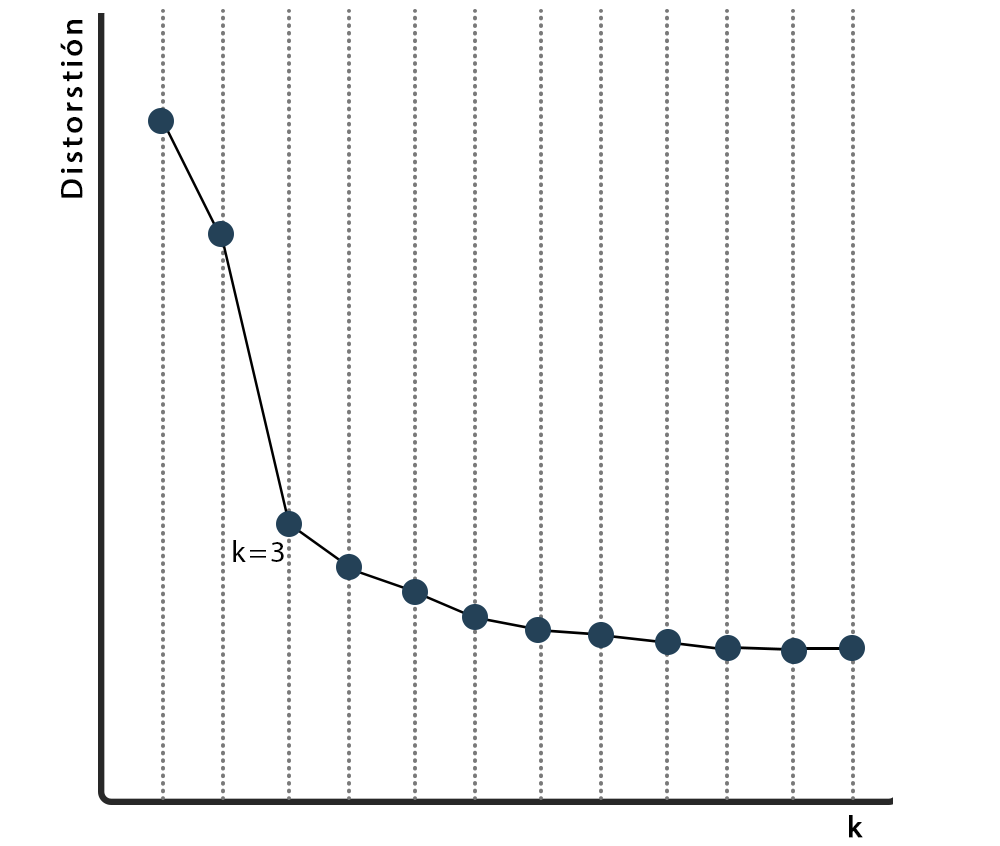
\includegraphics[width=0.75\linewidth]{imagenes/metodo-codo.png}
    \caption{Método del codo para la elección del parámetro \textit{k}}
    \label{fig:metodo-codo}
\end{figure}

\newpage

\subsubsection*{Orden de eficiencia de K-means}

Su orden de eficiencia es:

\vspace{-0.2cm}

\begin{equation}
    O(nkdi)
\end{equation}

donde \( n \) es el número de puntos de datos, \( k \) es el número de \textit{clusters}, \( d \) es la dimensión de los datos y \( i \) es el número de iteraciones hasta la convergencia. \\

\vspace{-3mm}

\subsubsection*{Librería sklearn para la implementación de K-means}

Puede aprovecharse la implementación del algoritmo K-means de la librería scikit-learn de Python \cite{datacamp_kmeans_2023}, la cual permite la normalización, ajuste y evaluación del modelo, así como la visualización de los resultados con un gran margen de personalización. \\

Consta de los siguientes parámetros de entrada y atributos de salida:

\begin{table}[H]
\centering
\footnotesize
\renewcommand{\arraystretch}{1.1}
\begin{tabularx}{\textwidth}{|p{3cm}|p{2.25cm}|X|}
\hline
\rowcolor{graylight}\texttt{Tipo} & \texttt{Nombre} & \texttt{Descripción} \\
\hline
\rowcolor{graylight}\multicolumn{3}{|c|}{\texttt{Parámetros de entrada}} \\
\hline
Parámetro & n\_clusters & Número de grupos en los que se dividen los datos. \\
\hline
Parámetro & init & Método que determina los centroides iniciales; permite las siguientes opciones:
\begin{itemize}
    \item \texttt{k-means++} \cite{arthur2007kmeans}: método por defecto.
    \item \texttt{random}: selecciona los centroides aleatoriamente.
    \item Matriz de centroides iniciales: se pueden pasar directamente.
\end{itemize} \\
\hline
Parámetro & n\_init & Número de repeticiones del algoritmo con diferentes centroides iniciales para obtener la mejor agrupación. \\
\hline
Parámetro & max\_iter & Número máximo de iteraciones para un conjunto dado de centroides iniciales. \\
\hline
\rowcolor{graylight}\multicolumn{3}{|c|}{\texttt{Atributos de salida}} \\
\hline
Atributo & cluster\_centers\_ & Array con los centroides de cada grupo, de dimensiones \( (k, m) \). \\
\hline
Atributo & labels\_ & Etiquetas de los elementos del conjunto agrupado, donde cada etiqueta i corresponde al centroide i en cluster\_centers\_. \\
\hline
Atributo & inertia\_ & Suma de las distancias al cuadrado de cada elemento a su centroide más cercano. \\
\hline
Atributo & n\_iter\_ & Número de iteraciones realizadas. \\
\hline
\end{tabularx}
\caption{Parámetros y atributos del algoritmo K-Means en sklearn}
\label{tab:kmeans}
\end{table}


\subsection{DBSCAN}
\label{dbscan}
Es el algoritmo de \textit{clustering} basado en densidad más utilizado en la actualidad \cite{10.1145/3068335} gracias a que no hace falta tener una gran base de conocimiento sobre los datos que se manejan y su uso es compatible con \textit{datasets} de gran tamaño.

Conceptualmente, \gls{DBSCAN} busca zonas que tengan una densidad alta y que estén alejadas de otras con una densidad más baja. 
Para ello se utilizan los términos \textit{neighbor}, que es un punto dentro del radio $\epsilon$ de otro punto, y \textit{neighborhood}, que es el conjunto de todos los puntos dentro del radio $\epsilon$ de un punto específico, incluyendo al punto mismo. \\

\begin{definition}
\shorthrule \vspace{0.1cm}
\\
El \textit{neighborhood} de un punto \( p \) conocido como \( N(p) \) puede definirse como:
\[
N(p) = \{ q \in D \mid \text{dist}(p, q) \leq \epsilon \}
\]
donde \( D \) es el conjunto de datos, \(\text{dist}(p, q)\) es la distancia entre los puntos \( p \) y \( q \), y \( \epsilon \) es el umbral de distancia.
\\ \vspace{0.1cm}
\fullhrule
\end{definition}

\subsubsection*{Pseudocódigo del algoritmo DBSCAN}

\begin{algorithm}[H]
\footnotesize
\caption{DBSCAN}
\textbf{Datos:} \textbf{D} conjunto de datos a agrupar, \textbf{eps} distancia máxima entre dos puntos vecinos, \textbf{minPts} mínimo número de puntos para formar un \textit{cluster}\\
\textbf{Resultado:} Datos agrupados en clusters
\begin{algorithmic}[1]
\State \textbf{Inicio;}
\State $C = 0$;
\For{\textit{cada punto} $P$ \textbf{de} \textit{D}}
    \If{$P$ \textit{no está en} \textit{visitados}}
        \State \textit{Marcar $P$ como visitado};
        \State $ptosVecinos = calcularRegion(P, eps)$;
        \If{$tamaño(ptosVecinos) < minPts$}
            \State \textit{marcar $P$ como ruido};
        \Else
            \State $C = próximo cluster$;
            \State $expandirCluster(P, ptosVecinos, C, eps, minPts)$;
        \EndIf
    \EndIf
\EndFor
\State \textbf{fin}
\end{algorithmic}
\end{algorithm}

Como se puede observar, se inicia desde un punto aleatorio y se verifica si en el radio \textit{eps} de ese punto existe un mínimo de puntos P. Si es así, se forma un \textit{cluster} y se vuelve a la primera etapa con uno de los puntos encontrados. Si no se alcanza el mínimo de puntos pero se ha llegado a través de un punto que sí cumplía esta condición, este formará parte del mismo \textit{cluster}. En caso de que no se pueda llegar al punto por medio de otros, no formará parte del \textit{cluster} y se clasificará como un nodo de tipo \textit{noise}.

\newpage

\subsubsection*{Parámetros del algoritmo \gls{DBSCAN}}

Los dos parámetros utilizados por este algoritmo son:

\begin{equation}
    DBSCAN ( eps, MinPts )
\end{equation}

donde

\begin{itemize}
    \item \textit{eps} es el radio máximo de un vecindario de un punto, es decir, la distancia máxima que se considera para definir los puntos vecinos.
    \item \textit{MinPts} es el número mínimo de puntos requeridos para formar un punto {\textcolor{darkgreen}{\textbf{core}}}. Un punto se considera un punto \textit{core} si hay al menos \textit{MinPts} puntos dentro de su vecindario (incluyendo el mismo punto).
\end{itemize}

\subsubsection*{Clasificación de puntos en un \textit{cluster} de \gls{DBSCAN}}

Los puntos se clasifican en tres tipos posibles, tal y como se describe en la Tabla \ref{tab:dbscan} y se ilustra en la Figura \ref{fig:puntos-dbscan}.

\begin{table}[H]
\centering
\footnotesize
\renewcommand{\arraystretch}{1.1}
\begin{tabularx}{\textwidth}{|p{3cm}|X|}
\hline
\rowcolor{graylight}\texttt{Tipo} & \texttt{Descripción} \\
\hline
\textbf{\textcolor{darkgreen}{\textbf{core}}} & Puntos interiores de un \textit{cluster} con un vecindario de radio $\epsilon$. \\
\hline
\textbf{\textcolor{blue}{\textbf{border}}} & Tienen menos de MinPts puntos en su vecindario de radio Epsilon, estando en el vecindario de algún punto \textcolor{darkgreen}{\textbf{core}}. \\
\hline
\textbf{\textcolor{red}{\textbf{noise}}} & Cualquier punto que no forma parte del \textcolor{darkgreen}{\textbf{core}} de un \textit{cluster} ni está en su frontera o \textcolor{blue}{\textbf{border}}. \\
\hline
\end{tabularx}
\caption{Clasificación de puntos en DBSCAN}
\label{tab:dbscan}
\end{table}

\vspace{-2mm}

\begin{figure}[H]
    \centering
    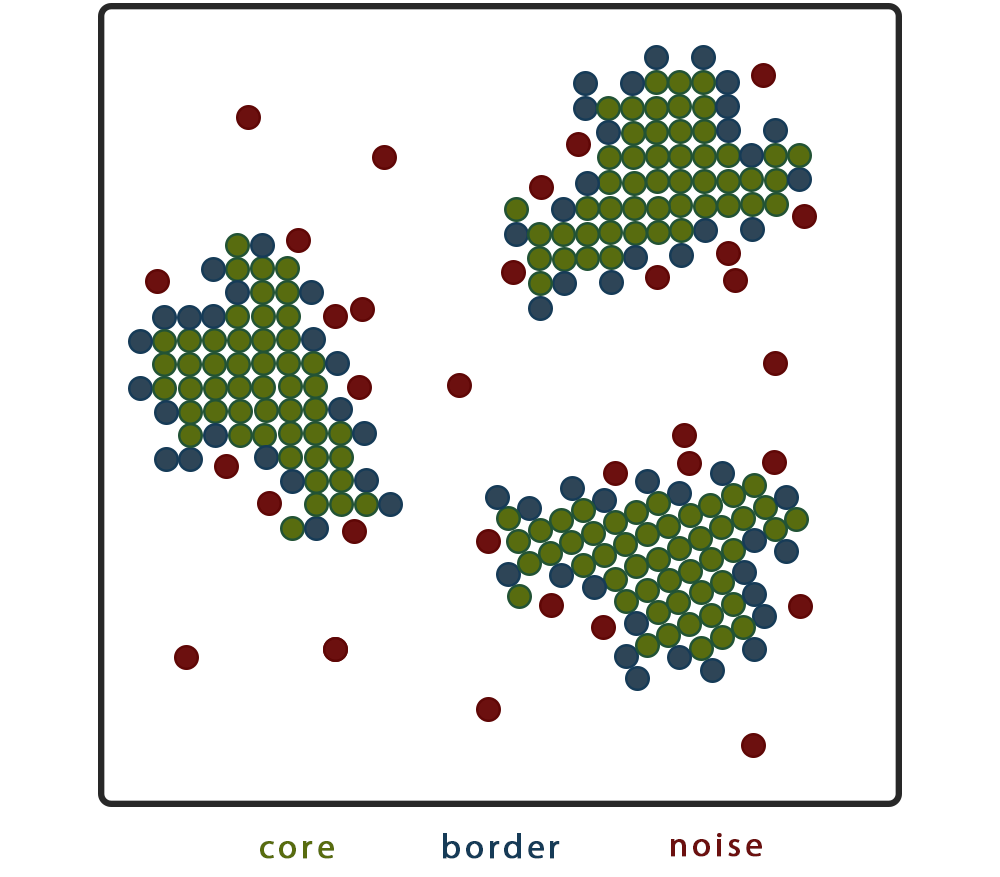
\includegraphics[width=0.725\linewidth]{imagenes/dbscan-points.png}
    \caption{Ejemplo de clasificación de puntos de algoritmo de \textit{clustering} \gls{DBSCAN}}
    \label{fig:puntos-dbscan}
\end{figure}

\subsubsection*{Orden de eficiencia de \gls{DBSCAN}}

Su orden de eficiencia es:

\vspace{-0.2cm}

\begin{equation}
    O(n \log n)
\end{equation}

donde \( n \) es el número de puntos de datos.

\subsection{Clustering Jerárquico} % clustering jerárquico. DHC También existe
\label{AHC}
También conocido como \textit{Agglomerative Hierarchical Clustering} \cite{Aggarwal2013}, este algoritmo jerárquico que agrupa datos de manera aglomerativa. Es decir, comienza tratando cada punto de datos como un clúster individual y, en cada paso, combina los dos clústeres más cercanos hasta que todos los puntos de datos pertenecen a un solo clúster.

El proceso del algoritmo se basa en la siguiente serie de pasos:

\begin{table}[H]
\footnotesize
\centering
\begin{tabular}{|l|p{12cm}|}
\hline
\rowcolor{graylight} \texttt{Paso} & \texttt{Descripción} \\
\hline
1 & Calcular la matriz de disimilitud entre todos los puntos de datos. \\
\hline
2 & Repetir los siguientes pasos hasta que quede un solo clúster: \\
\hline
3 & Fusionar los \textit{clusters} más cercanos \( C_a \) y \( C_b \). El nuevo \textit{cluster} tendrá una cardinalidad \( N_{a \cup b} = N_a + N_b \). \\
\hline
4 & Insertar una nueva fila y columna en la matriz de disimilitud que contenga las distancias entre el nuevo \textit{cluster} \( C_{a \cup b} \) y los \textit{clusters} restantes. \\
\hline
5 & Terminar cuando solo quede un \textit{cluster} máximo. \\
\hline
\end{tabular}
\caption{Pasos del algoritmo de Clustering Jerárquico Aglomerativo}
\end{table}


\vspace{-3mm}

\subsubsection*{Pseudocódigo del algoritmo \gls{AHC}}

\vspace{-3mm}

\begin{algorithm}[H]
\footnotesize
\caption{AHC}
\textbf{Datos:} \textbf{D} Agrupación de datos a amontonar\\
\textbf{Resultado:} Datos agrupados en un solo \textit{cluster} jerárquico
\begin{algorithmic}[1]
\State \textbf{Inicio;}
\State Calcular la matriz de disimilitud entre todos los puntos de datos;
\Repeat
    \State Fusionar los \textit{clusters} más cercanos $C_a \cup C_b$. Establecer la cardinalidad del nuevo \textit{cluster} como $N_{a \cup b} = N_a + N_b$;
    \State Insertar una nueva fila y columna que contenga las distancias entre el nuevo clúster $C_{a \cup b}$ y los \textit{clusters} restantes;
\Until{solo quede un \textit{cluster} máximo.}
\end{algorithmic}
\end{algorithm}

\vspace{-0.1cm}

\subsubsection*{Parámetros del algoritmo \gls{AHC}}

A diferencia de los anteriores, este algoritmo no requiere parámetros explícitos como K-means o \gls{DBSCAN}. En su lugar, la principal decisión que hay que tomar es la métrica de disimilitud \footnotemark utilizada para calcular las distancias entre \textit{clusters}, que puede ser:

\begin{itemize}
    \item Distancia simple (\textit{single linkage}): La distancia mínima entre puntos de diferentes \textit{clusters}. \\
    \item Distancia completa (\textit{complete linkage}): La distancia máxima entre puntos de diferentes \textit{clusters}.\\
    \item Distancia promedio (\textit{average linkage}): El promedio de todas las distancias entre puntos de diferentes \textit{clusters}.
\end{itemize}

\footnotetext{Es una medida que cuantifica cuán diferentes son dos elementos. En el contexto del \textit{clustering}, se utiliza para calcular la distancia entre puntos de datos o \textit{clusters}.}

\vspace{-3mm}

\subsubsection*{Orden de eficiencia de AHC}

El orden de eficiencia del algoritmo AHC es:

\vspace{-0.2cm}

\begin{equation}
    O(n^3)
\end{equation}

donde \( n \) es el número de puntos de datos. Este orden de eficiencia se debe al cálculo repetido de distancias entre todos los pares de clústeres a medida que se fusionan durante la construcción del árbol jerárquico. \\

Cuando se habla de \textit{clustering} jerárquico, debe definirse qué es un dendrograma. Se trata de una representación gráfica de los resultados del \textit{clustering} tal que en el eje vertical se muestra la distancia o disimilitud en la que se combinan los \textit{clusters}, mientras que en el eje horizontal se encuentran los puntos de datos, como se muestra en la Figura \ref{fig:dendrogram-example}. Esta visualización permite identificar la estructura del \textit{cluster} y decidir el número óptimo de \textit{clusters} al cortar el dendrograma a una altura específica.

\begin{figure}[H]
    \centering
    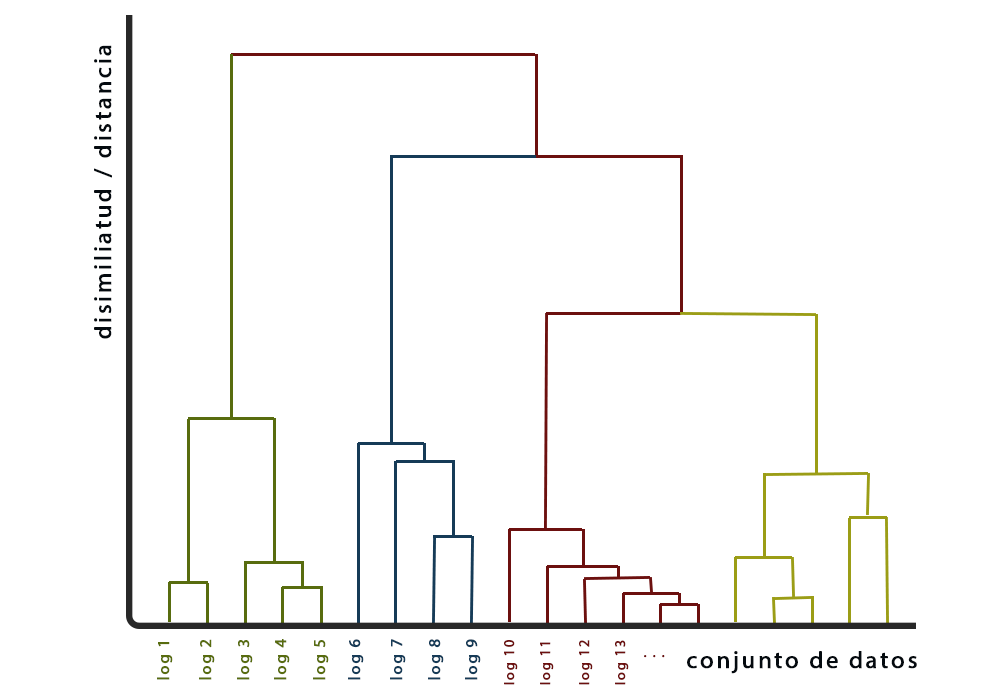
\includegraphics[width=0.8\linewidth]{imagenes/dendrograma.png}
    \caption{Ejemplo de un dendrograma para \gls{AHC}}
    \label{fig:dendrogram-example}
\end{figure}

\newpage

% ********************************************************************

\section{\textit{Set-up} experimental: tecnologías y herramientas}

\vspace{-1mm}

Para llevar a cabo la implementación del proyecto con la mayor precisión posible, se ha llevado a cabo un proceso minucioso de selección de las tecnologías y herramientas que se iban a utilizar.

\subsection{Herramientas para la simulación de ataques}

En primer lugar, ha sido necesario seleccionar uno de los múltiples \textit{frameworks} existentes basados en el marco adversario de  MITRE \gls{ATT&CK} para llevar a cabo la simulación de ataques a las máquinas y la posterior generación de grandes cantidades de \textit{logs} que pudiesen ser procesadas para generar un \textit{dataset}. Complementariamente, se han utilizado otras herramientas de explotación para enriquecer la cantidad de eventos generados a raíz de distintos ataques.

\vspace{-1mm}

\subsubsection*{Framework \gls{CALDERA}}

El \textit{framework} escogido ha sido \textbf{\gls{CALDERA}} \cite{caldera}, ya que permite emular la totalidad de técnicas y tácticas contempladas por el marco de MITRE, además de ofrecer una gran personalización. La versión utilizada ha sido la v5.0.0 "Magma" \cite{caldera_v500}, publicada el pasado 14 de febrero. A diferencia de las alternativas propuestas en la segunda sección del Estado del Arte (\ref{frameworks-mitre}), esta ha sido directamente desarrollada por MITRE, lo que la convierte en la solución opensource más estandarizada y utilizada en el entorno empresarial. 

Su funcionamiento está basado en la combinación de dos sistemas: \gls{ViRTS}, una infraestructura sofware usada para crear y emular adversarios de \textit{red-team}, y un modelo lógico denominado \gls{LAVA} que se encarga de determinar que acciones adversarias llevar a cabo. 

Por otro lado, la infraestructura de \gls{CALDERA}, instanciada por \gls{ViRTS}, se compone de dos elementos principales: el servidor maestro (ExtroViRTS) y los clientes de herramientas de acceso remoto (\gls{RAT}) en hosts ya infectados (IntroViRTS), como se observa en la Figura \ref{fig:caldera-infraestructure}. 

El proceso consta de los siguientes pasos \cite{gjerstad2022generating}:

\begin{enumerate}
    \item \textbf{Configuración inicial}: \gls{CALDERA} se configura de modo que un único host esté infectado con un \gls{RAT} de IntroViRTS, asegurando que la comunicación entre este \gls{RAT} y el servidor maestro ExtroViRTS sea fluida. 
    \item \textbf{Ampliación del control}: A partir de la infección inicial, \gls{CALDERA} utiliza el motor \gls{LAVA} para determinar las acciones a tomar. El servidor maestro ejecuta una instancia de LAVA para seleccionar una acción específica a ejecutar.
    \item \textbf{Ejecución de acciones}: El servidor maestro envía un comando a un \gls{RAT} específico en el campo, que ejecuta la acción seleccionada.
    \item \textbf{Retroalimentación y actualización}: El \gls{RAT} envía todos los detalles relevantes de la acción ejecutada de vuelta al servidor maestro.
    \item \textbf{Actualización de la base de conocimientos}: El servidor ExtroViRTS lleva a cabo la actualización de su base de conocimientos interna.
    \item \textbf{Selección de futuras acciones}: El servidor maestro continúa utilizando \gls{LAVA} para seleccionar futuras acciones que serán ejecutadas por los clientes IntroViRTS.
\end{enumerate}

\vspace{-3mm}

\begin{figure}[H]
    \centering
    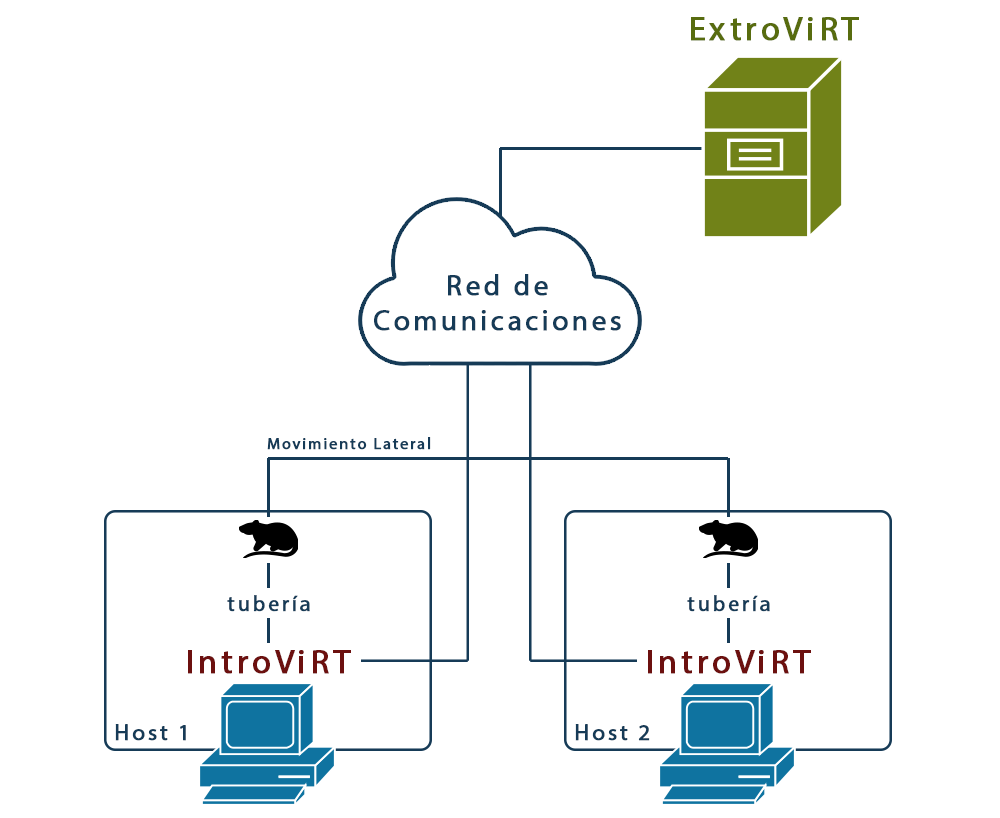
\includegraphics[width=0.75\linewidth]{imagenes/CALDERA-infraestructura.png}
    \caption{Infraestructura del framework \gls{CALDERA} \cite{gjerstad2022generating}}
    \label{fig:caldera-infraestructure}
\end{figure}

Este \textit{framework} emplea una terminología específica, cuyo entendimiento es vital para poder llevar a cabo un ataque. Como se muestra en la Tabla \ref{tab:caldera-terminologia}, distinguimos entre cuatro elementos principales:

\begin{table}[h]
\centering
\footnotesize
\begin{tabularx}{\linewidth}{|l|X|}
\hline
\rowcolor{graylight}\texttt{Término} & \texttt{Descripción} \\
\hline
Agentes & Aplicación software que se conecta de a CALDERA en intervalos regulares para obtener instrucciones. Cada agente se comunica con el servidor de CALDERA y se le asigna un ID único llamado \textit{paw}. Algunos ejemplos de agentes disponibles son Sandcat, Manx y Ragdoll. \\
\hline
Habilidades & Tácticas, técnicas y procedimientos específicos de ATT\&CK que se ejecutan en agentes activos. Cada habilidad incluye los comandos a ejecutar, las plataformas/ejecutores para el comando, cargas útiles y una referencia a los resultados de salida en el servidor de CALDERA. \\
\hline
Adversarios & Perfiles de amenazas predefinidos que consisten en un grupo de habilidades (\gls{TTP}s). Los perfiles pueden ayudar a determinar qué habilidades deberían ejecutarse al llevar a cabo una operación. \\
\hline
Operaciones & Ejecutan habilidades en grupos de agentes. \\
\hline
\end{tabularx}
\caption{Terminología utilizada por el \textit{framework} de \gls{CALDERA}}
\label{tab:caldera-terminologia}
\end{table}

En el próximo capítulo se documentará el proceso seguido para llevar a cabo la instalación y configuración del \textit{framework}.

\subsubsection*{Herramientas de ataque adicionales} \label{adicional-tools}

\gls{CALDERA}, según lo comentado anteriormente, basa su funcionamiento en la infección del host atacado mediante un \textit{payload} conocido como agente, es por ello que todos los ataques generados por este \textit{framework} están orientados a reconocimiento, movimiento lateral y otras operaciones de explotación y post-explotación. Por consiguiente, con la finalidad de aumentar la variedad de eventos recopilados en el \textit{dataset}, se hará uso de las siguientes herramientas de \textit{hacking} ético:

\begin{itemize}
    \item \texttt{Metasploit} \cite{Kennedy2011}: se trata del \textit{framework} más utilizado para ejercicios de \textit{pentesting}, es ampliamente conocido por facilitar la automatización de una amplia gama de ataques asociados a \gls{CVE}s. Cuenta con una gran base de datos, y su popularidad debe a la facilidad de uso para realizar ataques realistas y eficaces en entornos controlados.\\
    \item \texttt{Hydra} \cite{Beale2004}: es una herramienta de \textit{cracking} de contraseñas que destaca por su velocidad a través de opciones de ataques concurrentes mediante hebras, y su versatilidad, soportando múltiples protocolos de red. Es altamente efectiva en técnicas de fuerza bruta y ataques por diccionario.
\end{itemize}

\subsection{Virtualización de las máquinas víctima}

Para llevar a cabo la simulación de ataques, se investigó acerca de qué tecnología utilizar de cara al despliegue de \textit{hosts} que simularan una infraestructura operacional que hubiera sido vulnerada y tuviera un servidor central que almacenara internamente todos los eventos registrados. Las dos principales opciones eran las siguientes:

\begin{table}[h]
\centering
\footnotesize
\begin{tabularx}{\linewidth}{|l|X|}
\hline
\rowcolor{graylight}\texttt{Tecnología} & \texttt{Descripción} \\
\hline
Máquinas virtuales & Ofrecen un aislamiento completo del sistema operativo subyacente, lo que resulta en una mayor seguridad y estabilidad. Sin embargo, consumen más recursos y requieren más tiempo para configurarse y mantenerse en comparación con los contenedores. \\
\hline
Contenedores Docker & Permiten un despliegue rápido y eficiente, consumiendo menos recursos que las máquinas virtuales. Además, facilitan la portabilidad entre diferentes sistemas y plataformas. Sin embargo, ofrecen un aislamiento menor que las máquinas virtuales. \\
\hline
\end{tabularx}
\caption{Comparación de tecnologías de virtualización para la simulación de ataques}
\end{table}

Una tercera opción sería el uso de \gls{WSL} para realizar desde ahí la simulación de ataques, ya que desde el lanzamiento de la versión 2.0 se han implementado numerosas mejoras a nivel de aislamiento con respecto a Windows, y al mismo tiempo proporcionando cada vez una mayor funcionalidad, que previamente estaba muy limitada en la versión 1.0. 

Esto fue analizado el pasado 18 de mayo de 2024 en Hack-én por el investigador Sergio De Los Santos en su ponencia titulada \textit{\gls{WSL}: Windows Subsystem for Linux. Del odio al amor y del amor al odio}. En su libro recientemente publicado \cite{santos_wsl_2024} puede obtenerse mucha más información sobre el tema. 


\begin{figure}[H]
    \centering
    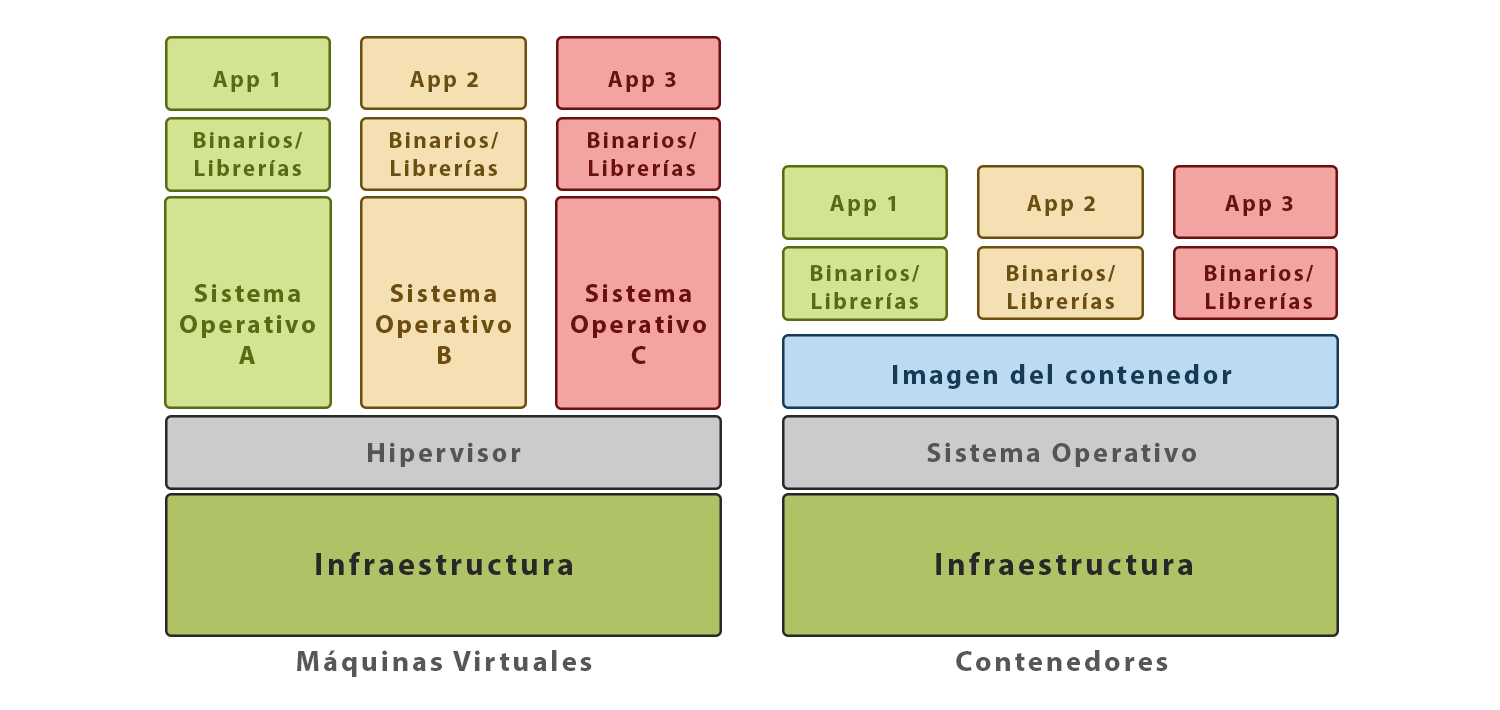
\includegraphics[width=1.1\linewidth]{imagenes/vms-vs-containers.png}
    \caption{Comparativa estructural de Máquinas Virtuales vs Contenedores}
    \label{fig:vm-vs-container}
\end{figure}

Finalmente, de las dos opciones ilustradas en la Figura \ref{fig:vm-vs-container} ha sido elegida la versión más ligera y simple: los contenedores \cite{vms_vs_containers}. Para el contexto de la simulación de ataques no suponía un problema que hubiese un menor aislamiento. Se llevaron a cabo pruebas de funcionalidad y rendimiento utilizando dos tipos de contenedores distintos.

El primero de ellos fue Alpine Linux \cite{alpine_linux}, que era la opción más ligera y rápida de generar a través de un Dockerfile, sin embargo tenía notables limitaciones y no representaba un entorno realista, ya que no se suele utilizar para servidores. La segunda opción fue un contenedor de Ubuntu Server \cite{ubuntu_server}, que ha resultado ser la elección definitiva, ya que sigue siendo una alternativa ligera pero con una utilidad suficiente como para llevar a cabo la simulación de ataques, y además es una distribución muy utilizada en cuanto a ingeniería de servidores respecta.

En el próximo capítulo se detallará cómo se ha llevado a cabo la implementación de los ficheros Dockerfile para levantar dichos contenedores.

\subsection{Librerías de Python utilizadas}

Python es actualmente el principal lenguaje de programación de alto nivel utilizado para cualquier actividad relacionada con análisis de datos, \gls{ML} o \gls{DL} \cite{subasi2020practical}. Es por ello que existen multitud de librerías que ofrecen una capa de abstracción para hacer uso de funcionalidades que se basan en el álgebra lineal y su implementación desde cero tendría un nivel de complejidad exponencial.

\vspace{-2mm}

\newpage

\subsubsection*{Librerías para el preprocesado de \textit{datasets}}

En primer lugar, para llevar acabo el preprocesado de \textit{datasets}, se han utilizado las siguientes librerías:

\begin{itemize}
\item \texttt{\gls{Pandas}}: Esta librería es una de las más conocidas en el análisis de datos. Proporciona estructuras de datos flexibles y potentes, conocidas como DataFrames, que facilitan la limpieza, transformación y análisis de grandes volúmenes de datos. Pandas permite cargar datos desde diversos formatos (CSV, Excel, SQL, etc.) y realizar operaciones complejas de agrupación, filtrado y agregación de manera eficiente. \\
\item \texttt{\gls{re}}: El módulo \textit{re} de Python proporciona soporte para expresiones regulares. Este permite buscar, sustituir y dividir cadenas de texto basándose en patrones específicos, lo cual resulta especialmente útil para el procesamiento de campos de \textit{logs}. \\
\item \texttt{\gls{CSV}}: La librería \textit{csv} se utiliza para leer y escribir archivos en formato \gls{CSV} (Comma-Separated Values). Este formato es el más utilizado para el análisis de datos y es compatible con muchas herramientas de análisis como las utilizadas en este proyecto para la implementación del \textit{clustering}. \\
\item \texttt{io}: El módulo \textit{io} de Python sirve para trabajar con flujos de datos en memoria, permitiendo la lectura y escritura de datos en diversos formatos sin necesidad de interactuar directamente con el sistema de archivos. Esto es útil para la manipulación temporal de datos durante el preprocesado.
\end{itemize}

El uso de estas librerías ha sido más que suficiente para realizar el preprocesado de los \textit{datasets} en un formato inicial de \texttt{.log}, ya que han permitido limpiar y posteriormente transformar los datos de manera eficiente de cara a su posterior análisis.

\subsubsection*{Librerías para la implementación del \textit{clustering}}

En segundo lugar, para la implementación de técnicas de \textit{clustering} en Python, se ha hecho uso de varias librerías que ofrecen un uso a alto nivel de algoritmos utilizados para la agrupación de datos como los estudiados anteriormente \ref{clustering}. Estas son:

\begin{itemize}
\item \texttt{Scikit-learn} (sklearn)\label{scikit}: Esta librería es una de las más populares para el aprendizaje automático en Python. Incluye una amplia gama de algoritmos de \textit{clustering}, como K-means, \glspl{DBSCAN} y \textit{clustering} jerárquico. Scikit-learn proporciona una interfaz sencilla y consistente para entrenar, evaluar y ajustar modelos, lo que facilita enormemente la integración de técnicas de \textit{clustering} en \textit{pipelines} de procesamiento de datos. \\
\item \texttt{NumPy}: Ofrece una poderosa estructura de datos en forma de arrays y matrices multidimensionales, y además permite realizar cálculos numéricos de forma eficiente sobre grandes volúmenes de datos, facilitando así la implementación de algoritmos de \textit{clustering} y otras técnicas de procesamiento de datos. \\
\item \texttt{Matplotlib}: Aunque no es una librería de \textit{clustering}, \textit{matplotlib} es fundamental para la visualización de los resultados del \textit{clustering}. Permite crear gráficos Y por tanto visualizar los resultados de los algoritmos de agrupación de cara a su análisis. \\
\item \texttt{Scipy}: Esta librería complementa a \textit{scikit-learn} proporcionando funciones adicionales para el análisis y manipulación de datos. Incluye herramientas para la implementación de \textit{clustering} jerárquico y otras técnicas similares. \\
\item \texttt{\gls{UMAP}-learn}: Tal y como indica su nombre, implementa la técnica de reducción de dimensionalidad que también se puede utilizar para el \textit{clustering}. \texttt{\gls{UMAP}} es especialmente útil para visualizar datos de alta dimensionalidad y descubrir estructuras subyacentes en los datos. Esto ha optimizado considerablemente la implementación del proyecto.  \\
\item \texttt{Tabulate}: Facilita la creación de tablas con diferentes estilos de formato de manera muy sencilla y rápida a partir de listas de datos o estructuras similares. Esta soporta texto simple, \gls{HTML}, LaTeX, y Markdown, lo cual resulta especialmente de cara al análisis de resultados.
\end{itemize}

El uso combinado de estas librerías ha permitido implementar de manera eficiente y robusta diversas técnicas de \textit{clustering}, que luego han sido utilizadas en los \textit{datasets} de \textit{logs} generados, para llevar a cabo el estudio de vectores de ataque.

\vspace{4mm}
\noindent\rule[-1ex]{\textwidth}{0.5pt}\\
\vspace{4mm}

En la Figura \ref{fig:diagrama-estructural} se muestra el diagrama estructural utilizado para llevar a cabo este Trabajo.

\newpage

\begin{landscape}   
    \noindent\hspace*{-2.7cm}
    \begin{minipage}{\linewidth}
        \begin{figure}[H]
            \centering
            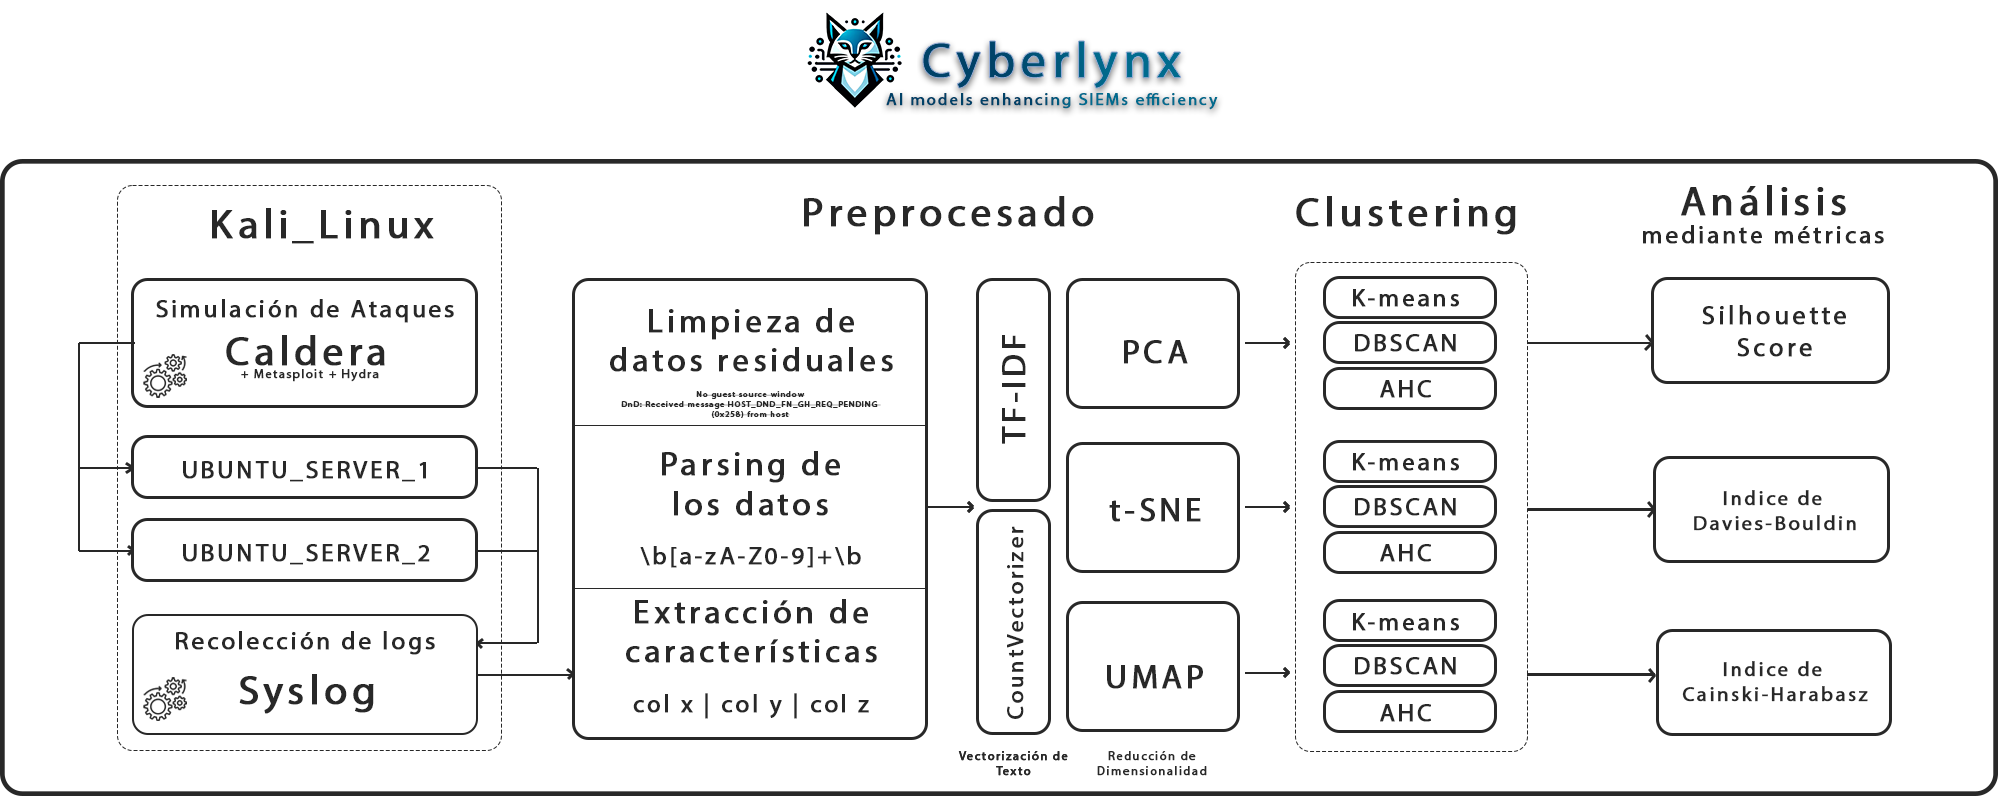
\includegraphics[width=1.3\linewidth, keepaspectratio]{imagenes/scheme-v4.png}
            \caption{Diagrama estructural del Trabajo de Fin de Grado}
            \label{fig:diagrama-estructural}
        \end{figure}
    \end{minipage}
\end{landscape}

\newpage

\chapter{Desarrollo e implementación}

En este capítulo se abordará cómo se ha llevado a cabo el proceso de implementación del proyecto, partiendo desde la preparación del entorno para la realización de ataques y posterior generación del \textit{dataset} de logs, siguiendo por cómo se ha preprocesado dicho \textit{dataset} y otros extraídos de fuentes públicas para la comparación de resultados, y finalmente la implementación de las distintas técnicas de \textit{clustering} y la selección de métricas para evaluar los resultados obtenidos.

% ********************************************************************

\section{Simulación de ataques y generación de logs}

A continuación, se verá en detalle cómo se han desarrollado los conjuntos de datos de \textit{logs} de Linux. En primer lugar, se ha realizado un \textit{dataset} de manera totalmente manual, y finalmente se ha hecho uso de un \gls{LLM} para la generación de un \textit{dataset} sintético y ya estructurado que simula dichos \textit{logs}.

\vspace{-3mm}

\subsection{Dataset Manual}

Como se ha comentado en capítulos anteriores, para la simulación de ataques se hará uso del framework de \gls{CALDERA} \cite{caldera}. Antes de mostrar este proceso paso a paso, es importante recalcar que toda la implementación de esta sección se hará sobre el sistema operativo Kali Linux 6.5.0-kali3-amd64 Debian \gls{GNU}/Linux  tal y como se indica en la Figura \ref{fig:uname-kali}, aunque podría ser emulado de forma equivalente en otras distribuciones de Linux.

\begin{figure}[H]
    \centering
    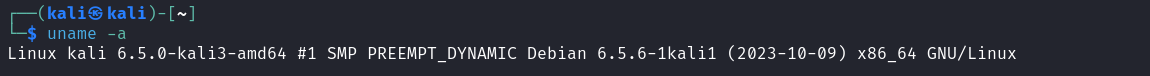
\includegraphics[width=1\linewidth]{imagenes/uname-kali.png}
    \caption{Distribución de Linux utilizada para la Simulación de ataques}
    \label{fig:uname-kali}
\end{figure}

Sobre este, colgarán 2 contenedores Docker con la distribución de Ubuntu Server que serán utilizados como máquinas víctima para llevar a cabo los ataques. Además del uso de este \textit{framework} de MITRE, se hará uso de otros servicios como Syslog, \gls{SFTP} o \gls{SSH}. La máquina Kali actuará como servidor central y por tanto los \textit{logs} de las máquinas que son objeto de ataque tendrán un flujo de salida hacia este, de modo que a través de la configuración de Syslog se irá formando un fichero \.log que dará forma al \textit{dataset} en formato \textit{raw}. Al mismo tiempo, por simplicidad, actuará como máquina atacante dentro de la misma subred que simula la infraestructura empresarial.

\vspace{-2mm}

\subsubsection*{Configuración del Servidor Syslog y Máquinas Víctima}

Con el fin de llevar a cabo la emulación de ataques sobre los contenedores y que los eventos generados se almacenaran en un único fichero, fue necesario diseñar la arquitectura del entorno, incluyendo los servicios utilizados,  ficheros de configuración necesarios, así como el orden a seguir para preparación. En primer lugar, se definió la arquitectura de modo que las máquinas involucradas fueran:

\begin{table}[H]
\footnotesize
\begin{tabularx}{\linewidth}{|l|X|}
    \hline
    \rowcolor{graylight}\texttt{Máquina} & \texttt{Descripción} \\
    \hline
    \texttt{KALI\_LINUX} & Máquina principal con el framework de \gls{CALDERA} instalado y servidor de Syslog para monitorizar los logs. \newline Virtualizado con Oracle \gls{VM} VirtualBox. \\
    \hline
    \texttt{UBUNTU\_SERVER\_1} & Primera máquina víctima, contenedor de Docker levantado sobre máquina Kali. \\
    \hline
    \texttt{UBUNTU\_SERVER\_1} & Segunda máquina víctima, contenedor de Docker levantado sobre máquina Kali. \\
    \hline
\end{tabularx}
\caption{Máquinas utilizadas para la simulación de ataques y recolección de \textit{logs}}
\label{tab:machines}
\end{table}

Cada una de las máquinas reenviará el flujo de \textit{logs} al servidor de Syslog ubicado en la máquina Kali. De tal modo, será posible almacenar en un mismo fichero los \textit{logs} de cada una, como se ilustra en la Figura \ref{fig:entorno-ataques}.

\vspace{2mm}

\begin{figure}[H]
    \centering
    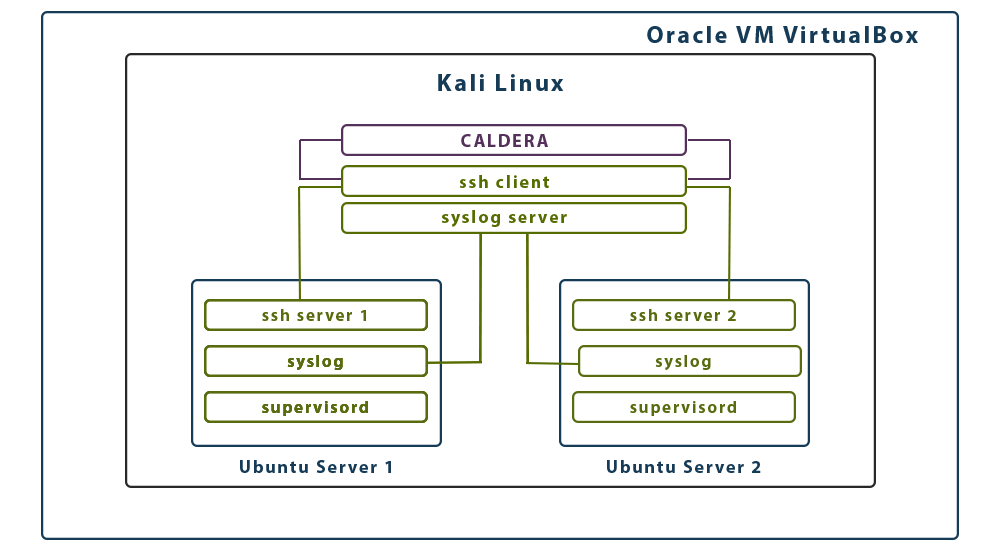
\includegraphics[width=1\linewidth]{imagenes/Enviromentv2.png}
    \caption{Arquitectura del entorno de simulación de ataques}
    \label{fig:entorno-ataques}
\end{figure}

\newpage

Se realizaron los siguientes pasos: \\

1. Acceder a la ruta donde se ubica el fichero Dockerfile y ejecutar el siguiente comando para construir la imagen \texttt{ubuntu-logger}:

\begin{mdframed}
\footnotesize
 \begin{minted}{docker}
docker build -t ubuntu-logger .
\end{minted}   
\end{mdframed}

2. Crear las máquinas a partir de la imagen generada:

\begin{mdframed}
\footnotesize
\begin{minted}{docker}
docker run -d --name ubuntu-logger-1 ubuntu-logger
docker run -d --name ubuntu-logger-2 ubuntu-logger
\end{minted}
\end{mdframed}

3. Iniciar una shell en ambas máquinas:

\begin{mdframed}
\footnotesize
\begin{minted}{docker}
docker exec -it ubuntu-logger-1 /bin/bash
docker exec -it ubuntu-logger-2 /bin/bash
\end{minted}
\end{mdframed}

Para construir las imágenes de los contenedores de Ubuntu Server \cite{ubuntu_server} se utilizó el siguiente fichero Dockerfile:

\begin{center}
\begin{mdframed}
\footnotesize
    \begin{minted}{docker}
# Se utiliza la imagen oficial de Ubuntu
FROM ubuntu:latest

# Evita preguntas al instalar paquetes
ARG DEBIAN_FRONTEND=noninteractive

# Actualiza los repositorios
RUN apt-get update
#Instala rsyslog, nano, iproute2, openssh-server y supervisor
RUN apt-get install -y rsyslog nano iproute2 curl openssh-server \
supervisor

# Configura rsyslog para enviar logs a máquina host y desactivar imklog
RUN sed -i 's/module(load="imklog")/#module(load="imklog")/' \
/etc/rsyslog.conf && echo '*.* @@172.17.0.1:514' >> /etc/rsyslog.conf

# Configura SSH para permitir acceso root con contraseña
RUN sed -i 's/#PermitRootLogin prohibit-password/PermitRootLogin yes/' \
/etc/ssh/sshd_config && echo 'root:root' | chpasswd

# Configuración de supervisord
COPY supervisord.conf /etc/supervisor/conf.d/supervisord.conf

# Expone los puertos necesarios para syslog y SSH
EXPOSE 514 22

# Configura supervisord como el comando principal
CMD ["/usr/bin/supervisord"]
    \end{minted}
\end{mdframed}
\end{center}

\newpage

A continuación, es necesario editar el fichero \texttt{supervisord.conf} en los contenedores. Este, utilizado para la configuración de  \texttt{supervisord}, gestiona los procesos del sistema, asegurando que los servicios definidos se inicien y mantengan en ejecución, concretamente \texttt{ssh} y \texttt{rsyslog}. 

\begin{center}
\begin{mdframed}
\footnotesize
    \begin{minted}{bash}
[supervisord]
nodaemon=true

[program:sshd]
command=/usr/sbin/sshd -D

[program:rsyslogd]
command=/usr/sbin/rsyslogd -n
    \end{minted}
\end{mdframed}
\end{center}

Por otro lado, el fichero de configuración \texttt{rsyslog.conf} utilizado en la máquina Kali Linux define cómo se manejan los registros de las máquinas Ubuntu Server 1 y Ubuntu Server 2. 

Este permite la recolección y almacenamiento de \textit{logs} provenientes de estas, que están dentro de la misma subred. Dicho fichero debe de tener activos los módulos de \gls{TCP} y \gls{UDP} para que la transferencia de \textit{logs} se realice correctamente:

\begin{center}
\begin{mdframed}
\footnotesize
    \begin{minted}{bash}
# /etc/rsyslog.conf configuration file for rsyslog

module(load="imuxsock")
module(load="imklog")

module(load="imudp")
input(type="imudp" port="514")

module(load="imtcp")
input(type="imtcp" port="514")

    \end{minted}
\end{mdframed}
\end{center}

Además, es necesario añadir la siguiente línea al final del fichero para que almacene todos los tipos de ficheros de \textit{log} en un único archivo \texttt{dataset-raw.log}:

\begin{center}
\footnotesize
\begin{mdframed}
    \begin{minted}{bash}
*.* /var/log/dataset-raw.log
    \end{minted}
\end{mdframed}
\end{center}

Finalmente, es necesario que el fichero \texttt{rsyslog.conf} de los contenedores tenga el siguiente contenido, para que se envíen los \textit{logs} a la máquina Kali:

\begin{center}
\begin{mdframed}
\footnotesize
    \begin{minted}{bash}
# /etc/rsyslog.conf configuration file for rsyslog

module(load="imuxsock") # provides support for local system logging
module(load="imklog" permitnonkernelfacility="on")

$IncludeConfig /etc/rsyslog.d/*.conf
    \end{minted}
\end{mdframed}
\end{center}


\newpage

Es necesario añadir al final del fichero las siguientes líneas:

\begin{center}
\begin{mdframed}
\footnotesize
    \begin{minted}{bash}
*.* @@172.17.0.1:514
cron,kern,mail,user,auth,authpriv.* @@172.17.0.1:514
    \end{minted}
\end{mdframed}
\end{center}

Estas especifican la redirección de los \textit{logs} generados en los contenedores hacia el servidor de syslog centralizado, en este caso, la máquina Kali Linux con la dirección \gls{IP} \texttt{172.17.0.1} a través del puerto \texttt{514}. 

La primera línea indica que todos los mensajes de \textit{log}, independientemente de su nivel de severidad o su origen, deben ser enviados al servidor central. Por otro lado, la segunda, refuerza esta configuración para logs específicos generados por las \textit{facilities} \ref{tab:syslog_facilities} \texttt{cron}, \texttt{kern}, \texttt{mail}, \texttt{user}, \texttt{auth}, y \texttt{authpriv}.

\subsubsection*{Simulación de Ataques con \gls{CALDERA}}

Una vez se ha instalado y configurado correctamente el \textit{framework} de \gls{CALDERA} siguiendo la documentación del Anexo \ref{caldera-conf}, puede llevarse a cabo la simulación de ataques sobre los contenedores \texttt{UBUNTU\_SERVER\_1} y \texttt{UBUNTU\_SERVER\_2}. Dentro de la interfaz web del \textit{framework},simplemente basta con acceder a la sección de operaciones y hacer click sobre el botón de \texttt{Start} para iniciar la operación. La principal ventaja de este \textit{framework} es que la interfaz proporciona una monitorización en tiempo real de la ejecución de las operaciones, de modo que puedan verse los resultados que van obteniéndose, así como el orden de las tácticas y técnicas empleadas en dicho proceso de ataque.

\begin{figure}[H]
    \centering
    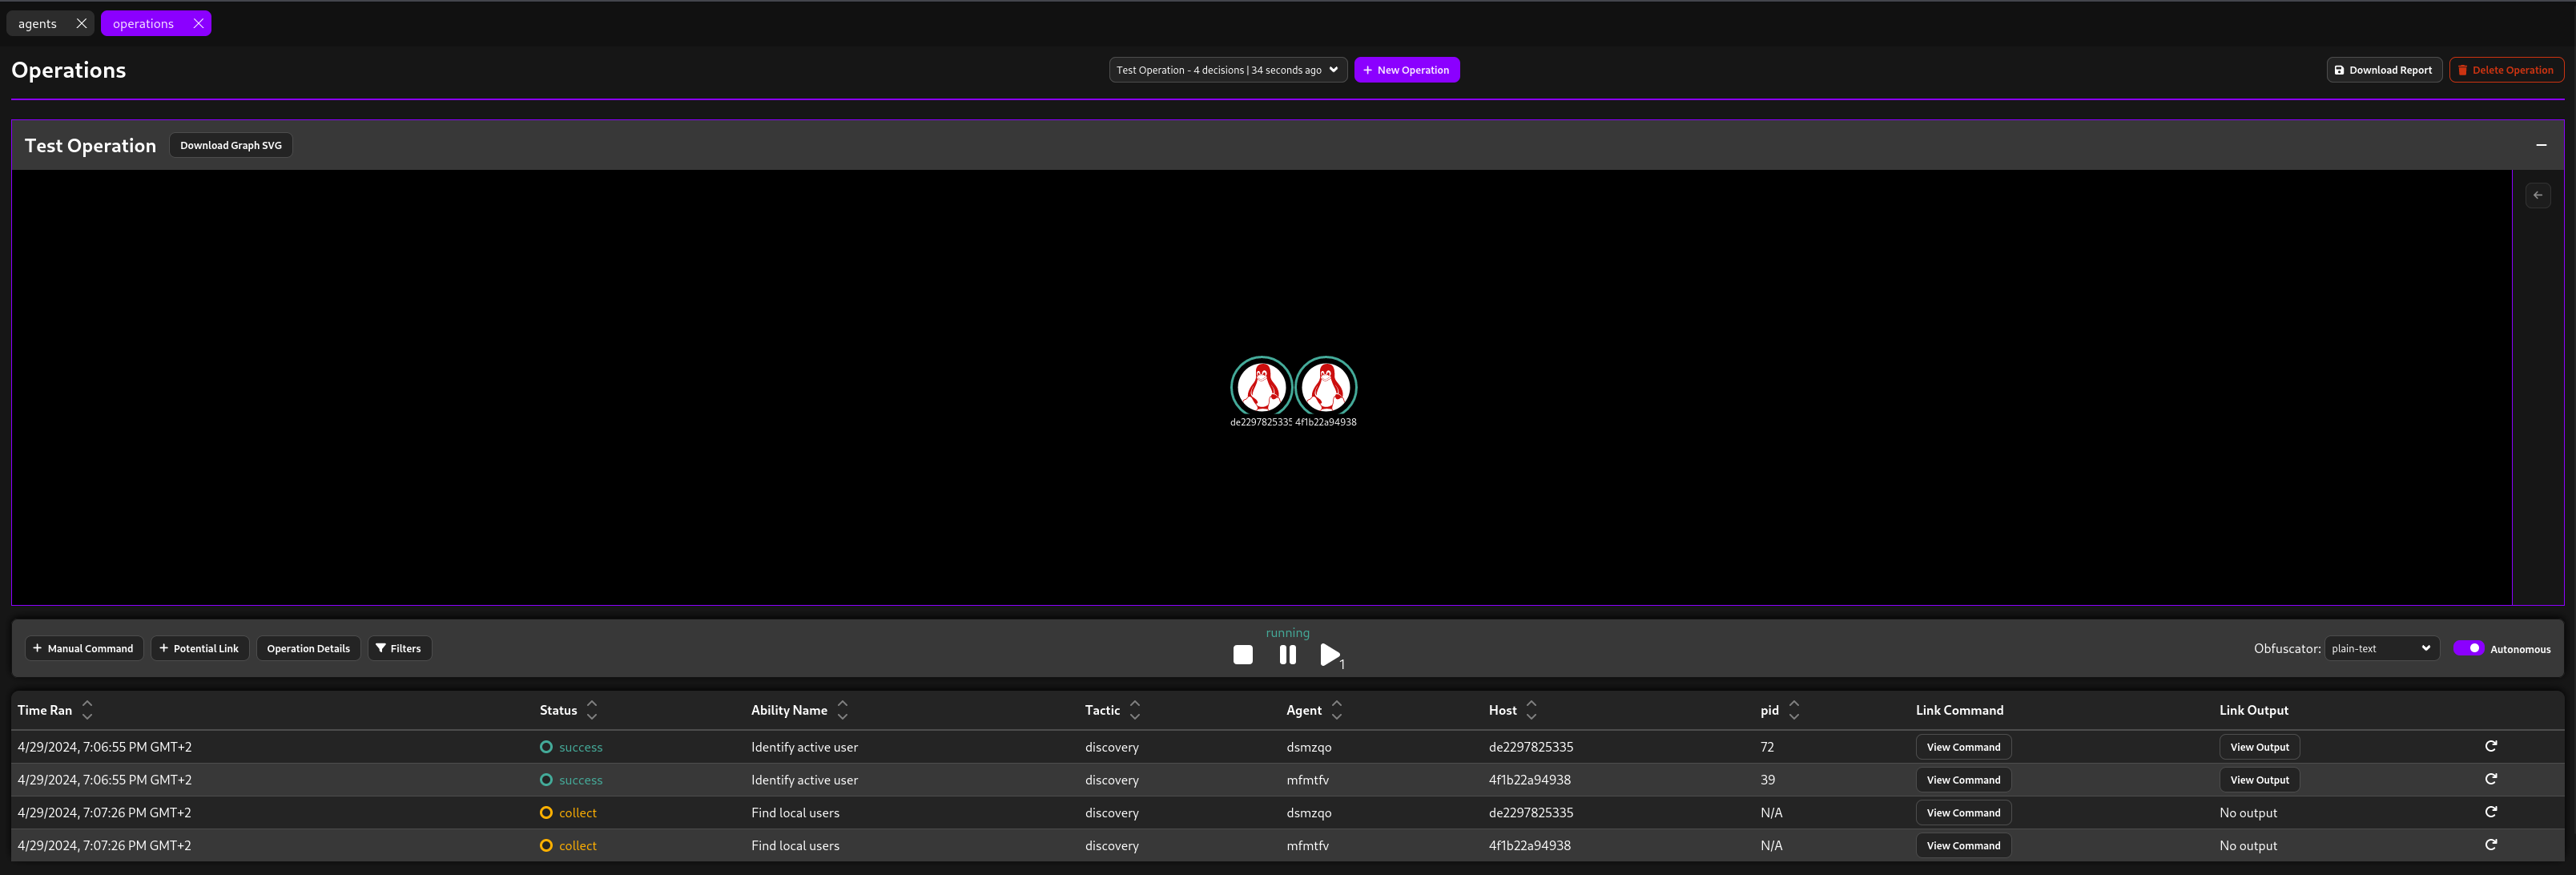
\includegraphics[width=1\linewidth]{imagenes/operation-start.png}
    \caption{Ejemplo de ejecución de una operación de Discovery con \gls{CALDERA}}
    \label{fig:operation-start}
\end{figure}

Tal y como se muestra en la Figura \ref{fig:operation-start}, el panel de operaciones una vez iniciado el ataque se divide en dos zonas. En primer lugar, la zona superior muestra las máquinas que están siendo atacadas y el tipo de sistema operativo de estas. En este caso son los dos contenedores de \texttt{Ubuntu Server}. En segundo lugar, la zona inferior detalla la información relativa al ataque, como es el tiempo de ejecución, el estado de la operación (p.e. \textit{success} o \textit{collect}), el nombre de la habilidad asociada, la táctica utilizada, el agente asociado al \textit{host}, el identificador del host, el \texttt{ID} del proceso e incluso el comando utilizado y su \textit{output} generado. 

Al mismo tiempo que se llevaban a cabo las operaciones, se fueron almacenando los eventos de \textit{logs} en las máquina víctima y enviándose de forma síncrona al servidor Syslog de la máquina \texttt{KALI\_LINUX}, como se muestra en la Figura \ref{fig:log-monitoring-syslog}. 

\begin{figure}[H]
    \centering
    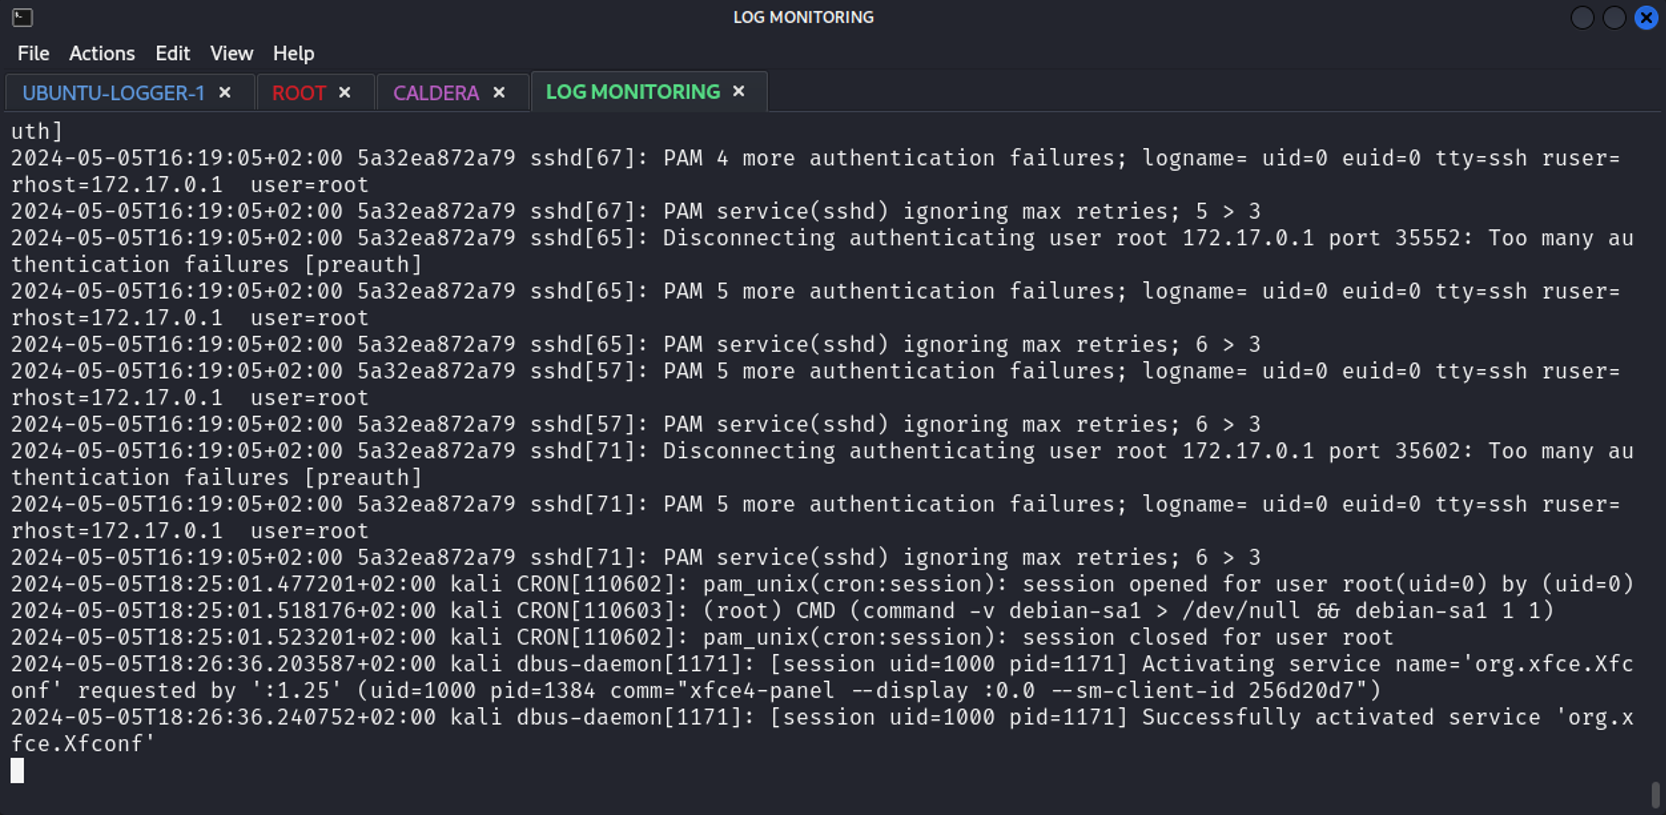
\includegraphics[width=1\linewidth]{imagenes/log-monitoring-syslog.png}
        \caption{Monitorización de \textit{logs} generados en máquinas víctima por operaciones}
    \label{fig:log-monitoring-syslog}
\end{figure}

\subsubsection*{Simulación de Ataques con otras herramientas}

Una vez efectuados los ataques en la infraestructura de red interna a través de \gls{CALDERA}, se llevó a cabo adicionalmente una serie de ataques adicionales a través de intentos de acceso externo mediante varias herramientas distintas indicadas anteriormente en \ref{adicional-tools}: \texttt{Metasploit} e \texttt{Hydra}. El proceso para cada una de ellas fue el siguiente: \\

En el caso de \texttt{Hydra}, se llevó a cabo un ataque por diccionario al servicio de \gls{SSH} como el mostrado en la Figura \ref{fig:hydra-ssh}, utilizando uno de los disponibles en la carpeta \texttt{/usr/share/wordlists/} de cualquier distribución \texttt{Kali}, en este caso el famoso diccionario \textit{Rockyou} \cite{kanta2022novel}. El comando utilizado fue:

\begin{center}
\begin{mdframed}
\scriptsize
    \begin{minted}{bash}
    hydra -l test-user -P /usr/share/wordlists/rockyou.txt.gz ssh://172.17.0.2
    \end{minted}
\end{mdframed}
\end{center}

\begin{figure}[H]
        \centering
        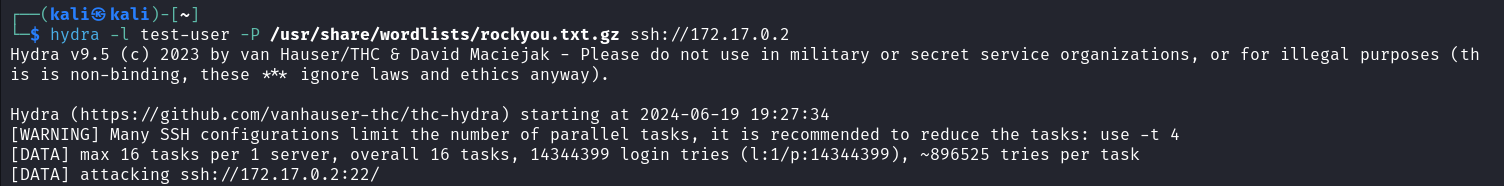
\includegraphics[width=1\linewidth]{imagenes/hydra-attack.png}
        \caption{Ataque por diccionario a servicio \gls{SSH} mediante Hydra}
        \label{fig:hydra-ssh}
\end{figure}

A continuación, se utilizó un \textit{scanner} de \texttt{Metasploit} para intentar enumerar usuarios de \gls{SSH} de las máquinas víctima. Para ello, se utilizaron los siguientes comandos:

\begin{center}
\begin{mdframed}
\scriptsize
    \begin{minted}{bash}
msfconsole # abrir una instancia de Metasploit
use auxiliary/scanner/ssh/ssh_enumusers # seleccionar script
set rhosts 172.17.0.2 # indicar la IP objetivo
set user_file /usr/share/wordlists/rockyou.gz # indicar el diccionario utilizado
run # ejecutar el ataque
    \end{minted}
\end{mdframed}
\end{center}

Finalmente, como se muestra en la Figura \ref{fig:metasploit-users}, se usa la técnica \textit{Malformed Packet}, que consiste en enviar paquetes formados incorrectamente a un servidor para probar forzar errores en el manejo de dichos paquetes y obtener información aparentemente oculta o inaccesible.

\begin{figure}[H]
    \centering
    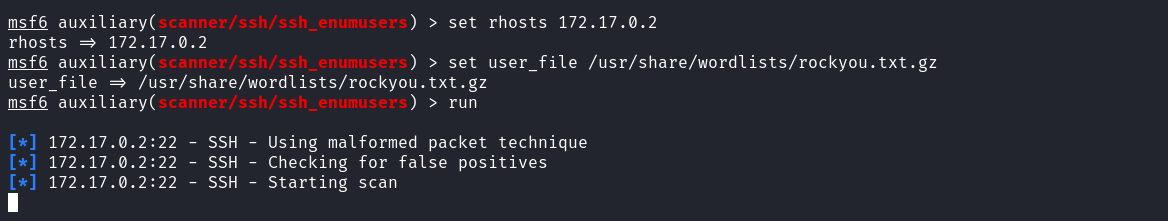
\includegraphics[width=1\linewidth]{imagenes/metasploit-attack.png}
    \caption{Ataque con Metasploit para enumeración de usuarios en un servidor \gls{SSH}}
    \label{fig:metasploit-users}
\end{figure}

\subsection{Dataset Sintético}

En el caso del conjunto de datos generado de manera sintética, se ha realizado por medio de la funcionalidad de análisis de datos utilizada por el LLM de OpenAI multimodal (\gls{GPT}4o). Para ello se ha hecho uso de técnicas de \textit{prompt engineering}, de modo que su estructura fuese equivalente a la del anterior \textit{dataset} ya preprocesado tal y como se especifica al final de la próxima sección \ref{fig:dataset-preprocesado}.

Este modelo es capaz de generar como salida un fichero de texto. Además, el \textit{notebook} que utiliza para generarlo puede ir readaptándose dinámicamente en base a las indicaciones que se van haciendo para ajustarlo al resultado deseado. Otra ventaja que presenta es la opción de adjuntar en el \textit{prompt} un fichero, de modo que si de añade un ejemplo del resultado esperado del conjunto de datos, como el generado anteriormente, el modelo razonará con más claridad como debe implementar las celdas de código. 

\begin{tcolorbox}[colframe=blue!25!white, colback=blue!10!white, title={\color{blue}\footnotesize \texttt{Prompt GPT4o - Generación Dataset Sintético}}]
\footnotesize
\textit{"Genera un archivo en formato \gls{CSV} que contenga 5000 registros, cada uno simulando un log de Linux orientado a la detección de vectores de ataque en sistemas de seguridad. Este dataset debe incluir una variedad ampliada de mensajes típicos encontrados en logs reales, adaptados para reflejar diversos tipos de actividades sospechosas y ataques, tales como intentos de acceso SSH, fallos de autenticación, alertas de kernel, y errores en aplicaciones y servicios de red. Cada log debe estar compuesto por las siguientes columnas, ajustándose al formato especificado en tu archivo de referencia: YYYY, MM, DD, hh, mm, Hostname, Service, User, IP, Port, Keyword, Interface, UID, Action, Protocol, Component, Severity, Type, Thread ID, Message.} \\
\end{tcolorbox}

\begin{tcolorbox}[colframe=blue!25!white, colback=blue!10!white, title={\color{blue}\footnotesize \texttt{Prompt GPT4o - Generación Dataset Sintético II}}]
\footnotesize
\textit{Incluye en los registros una mezcla de eventos legítimos y maliciosos, asegurando que los mensajes y tipos de errores sean coherentes con el protocolo y el servicio implicado (por ejemplo, mensajes ICMP relacionados con problemas de red y mensajes SSH relacionados con la autenticación). Asegúrate de que los datos sean variados y realistas para facilitar el análisis y la detección de patrones anómalos en aplicaciones de aprendizaje automático.} \\
\end{tcolorbox}

\begin{tcolorbox}[colframe=blue!25!white, colback=blue!10!white, title={\color{blue}\footnotesize \texttt{Prompt GPT4o - Generación Dataset Sintético III}}]
\footnotesize
\textit{El dataset debe ser guardado como} \verb|'06_Synthetic-logs-5k.csv'|\textit{, y cada entrada debe ser única para evitar redundancias y mejorar la calidad del mismo de cara a pruebas y entrenamiento de modelos."} \\

Por ejemplo:

\begin{tcolorbox}[colframe=white, colback=white, top=1mm, bottom=1mm, boxrule=0pt]
    \texttt{2024	05	05	09:38	f6194a3d2d4d	sshd[90]: test  172.17.0.1 	Invalid user test from 172.17.0.1 port 34132}
\end{tcolorbox}
\end{tcolorbox}

\vspace{2mm}

Además de los anteriores, fue necesario indicar 4 \textit{prompts} adicionales para ajustar más el formato del \textit{dataset} obtenido. Finalmente, se obtuvo el conjunto de datos que se muestra en la Figura \ref{fig:synthetic-dataset}, el cual incluye los veinte campos indicados, con una gran variedad de eventos y con una completitud significativa. 

\begin{figure}[H]
    \centering
    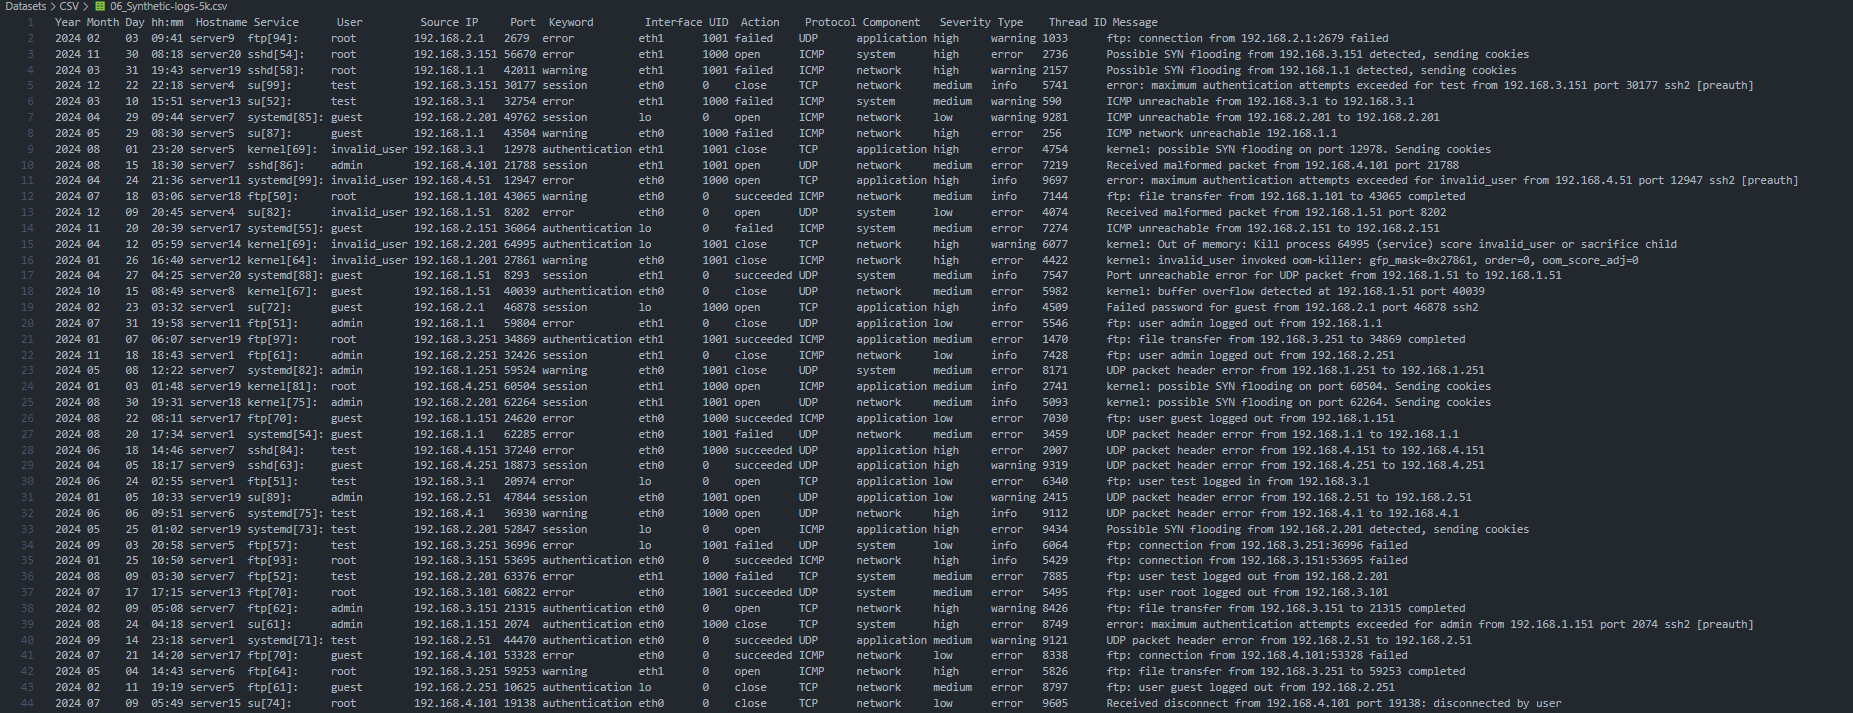
\includegraphics[width=1\linewidth]{imagenes/synthetic-dataset.png}
    \caption{Resultado del \textit{dataset} generado de forma sintética.}
    \label{fig:synthetic-dataset}
\end{figure}

Como se discute en el \textit{paper} de Krundyshev et. al \cite{inproceedings}, el uso de \textit{datasets} sintéticos en ciberseguridad actualmente es esencial para entrenar y evaluar modelos de detección de incidentes. Estos permiten simular una amplia gama de escenarios de ataque y actividades maliciosas que pueden no estar presentes en los datos reales debido a la rareza o sensibilidad de los incidentes. Además, ayudan a preservar la privacidad y la seguridad de los datos reales, mientras proporcionan un entorno controlado para experimentar y mejorar los modelos de detección. 


\newpage

% ********************************************************************

\section{Preparación de los \textit{dataset}s}


Una vez generado el \textit{dataset} original en formato \texttt{.log}, es necesario llevar a cabo un proceso de preprocesamiento de modo que pueda ser interpretado correctamente por los modelos de análisis de datos. Este proceso se tiene que realizar de manera equivalente para los otros \textit{datasets} que se han utilizado para hacer una comparativa y así enriquecer el análisis de posibles vectores de ataque. Se ha dividido en los siguientes pasos:

\begin{itemize}
    \item Limpieza del conjunto de datos: se eliminarán los eventos que se consideren residuales y no resulten útiles para el proceso de entrenamiento. Sin embargo, no se eliminarán todos los \textit{logs} que no estén relacionados con un ataque simulado, ya que la idea es poder generar agrupaciones de distintos \textit{logs} y ver cuáles de estas pertenecen a ataques, para que todo sea del modo más fidedigno posible a la realidad. 
    \item Preprocesamiento de los datos: el formato original de los \textit{logs} no es práctico para su análisis, por lo que será necesario transformarlo a un fichero \gls{CSV}, un formato más estandarizado para estas técnicas de \textit{clustering} y hacer técnicas de \textit{parsing} y normalización del texto.
    \item Extracción de características: en línea con el ítem anterior, será necesario extraer nuevos campos para facilitar el agrupamiento de \textit{logs} en base a características comunes.
\end{itemize}

A continuación se detalla cómo se han hecho cada uno de los pasos anteriores.

\vspace{-3mm}

\subsubsection*{Limpieza del conjunto de datos} % Dataset cleaning

En primer lugar, se suprimieron una gran cantidad de \textit{logs} redundantes y a su vez secuencialmente repetitivos para el problema a resolver, es decir, aquellos eventos generados en varias ocasiones que no aportaban al conjunto de datos. Este proceso se hizo manualmente examinando las aproximadamente nueve mil líneas de \textit{logs} y parseando a través de la técnica de \textit{search \& replace}. En la Figura \ref{fig:residual-logs} se muestra un ejemplo de \textit{logs} etiquetado como residual.

\vspace{-1mm}

\begin{figure}[H]
    \centering
    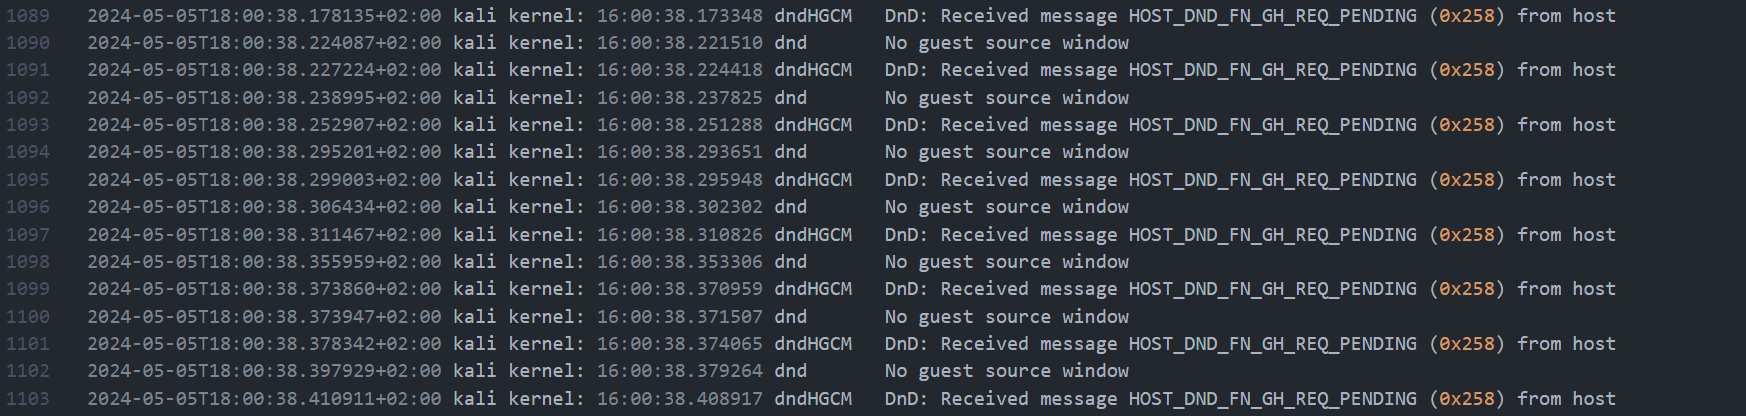
\includegraphics[width=1\linewidth]{imagenes/logs-residuales.png}
    \caption{Ejemplo de \textit{logs} residuales del conjunto de datos}
    \label{fig:residual-logs}
\end{figure}

\vspace{-5mm}

\begin{center}
\begin{mdframed}
\footnotesize
    \begin{minted}{bash}
No guest source window
DnD: Received message HOST_DND_FN_GH_REQ_PENDING (0x258) from host
    \end{minted}
\end{mdframed}
\end{center}

\vspace{-2mm}

Estos eventos están relacionados con un intento reiterado de realizar la operación de \gls{DnD} (\textit{drag \& drop}), pero que no se ha podido realizar debido a que no se ha encontrado la ventana de origen en el sistema invitado o \textit{guest}, un \textit{log} muy común en máquinas virtuales. También se han eliminado otros eventos relacionados con actividades de \textit{booting} de \gls{VM}s.

A través de este proceso, se consigue llevar a cabo un cierto balanceo de clases, lo cual es crucial para un buen rendimiento en el análisis de un \textit{dataset}. En el contexto de los conjuntos utilizados para este proyecto, el volumen de datos no es significativamente grande, sin embargo sería interesante usar algún algoritmo de balanceo \cite{garcia2021comparativa} en caso de enfrentarnos a conjuntos de datos mayores. Para ello se podrían utilizar algunos de los siguientes:

\begin{table}[H]
\centering
\footnotesize
\begin{tabularx}{\linewidth}{|>{\hsize=0.6\hsize}X|>{\hsize=1.4\hsize}X|}
\hline
\rowcolor{graylight}\texttt{Tipo} & \texttt{Descripción} \\
\hline
Sobremuestreo (\textbf{\textit{Oversampling}}) & Aumenta la cantidad de muestras en las clases menos representadas. El método más conocido es \gls{SMOTE} \cite{spositto2020smote}, donde se generan ejemplos sintéticos (no duplicados) mediante la interpolación entre ejemplos existentes de la clase minoritaria. \\
\hline
Submuestreo (\textbf{\textit{Undersampling}}) & Reduce la cantidad de muestras en las clases sobrerepresentadas. Este método puede llevar a una pérdida de información importante, pero es útil cuando hay un volumen muy alto de datos. \\
\hline
Combinación de sobremuestreo y submuestreo & Utiliza ambos métodos para equilibrar el conjunto de datos. Por ejemplo, se puede aplicar submuestreo a la clase mayoritaria y sobremuestreo a la clase minoritaria para lograr un balance. \\
\hline
Ensemble de modelos (\textbf{\textit{Ensemble methods}}) & Crea múltiples modelos (como árboles de decisión) en diferentes subconjuntos del conjunto de datos original, donde cada subconjunto refleja un balance de clases más equitativo. Técnicas como Balanced Random Forest o EasyEnsemble aplican esta idea. \\
\hline
Modificar pesos de clases (\textbf{\textit{Class weights modification}}) & Da más peso a la clase minoritaria durante el entrenamiento del modelo, lo cual puede influir en el algoritmo de aprendizaje para que preste más atención a la clase minoritaria. \\
\hline
\end{tabularx}
\caption{Técnicas de balanceo de clases para grandes conjuntos de datos}
\end{table}


\subsubsection*{Preprocesamiento de los datos}

Una vez los \textit{datasets} habían sido limpiados de \textit{logs} residuales, se pasó a la fase de preprocesamiento. Esta fase tuvo un primer enfoque mediante el cual los ficheros \textit{raw} se transformaron a un fichero \gls{JSON}.

El proceso fue muy similar para los conjuntos de datos utilizados. En el caso de los \textit{datasets} Linux\_2k \ref{Linux_2k} y el generado manualmente, se hizo uso de un mismo \textit{script}. Dicho código se adaptó levemente para poder utilizarse en los \textit{datasets} de \gls{BGL} (\ref{BGL}) y \gls{HDFS} (\ref{HDFS}). La principal diferencia entre estos fue el tratamiento del campo \textit{timestamp}, ya que los formatos eran ligeramente distintos, tal y como se explica en el capítulo cuarto (\ref{fig:linux-log-structure}).

\newpage

Para el primer paso, el \textit{script} realizaba un \textit{parsing} contenido para crear un diccionario con cuatro etiquetas por cada \textit{log}, de modo que se consiguiera la siguiente estructura:

\begin{center}
\begin{mdframed}
\footnotesize
    \begin{minted}{python}
{
    "timestamp": "2024-05-05T09:38:32+02:00",
    "hostname": "f6194a3d2d4d",
    "service": "sshd[90]:",
    "message": "pam_unix(sshd:auth): check pass; user unknown"
}
    \end{minted}
\end{mdframed}
\end{center}

Una vez todos los \textit{datasets} tenían este formato unificado, ya resultaba más fácil realizar el tratamiento de los campos para la extracción de características y generar nuevas columnas. 

\subsubsection*{Extracción de características}

Partiendo de los conjuntos de datos en formato \gls{JSON}, se continuó con el preprocesado. Se llevaron a cabo simultáneamente varios pasos \footnotemark para la extracción de características:


\begin{itemize}
    \item Normalización de los campos: principalmente, se normalizó el contenido del \textit{timestamp}, de modo que se mostrase con un formato equivalente. Este paso significó una leve pérdida de precisión en algunos de los datasets, que registraban también los segundos, microsegundos o bien la zona horaria asociada a la hora.
    \item Paso de \gls{JSON} a \gls{CSV}: mediante un \textit{notebook} de \textit{Jupyter} se llevó a cabo la transformación de los \textit{datasets} al formato matricial separado por comas. De esta manera, cada fila representaba un evento y cada columna una característica.
    \item Extracción de nuevos campos: a partir de los campos de \textit{timestamp} y \textit{message} se generaron nuevas columnas que mejorarían el potencial de estos para ser analizados y estudiados a continuación.
\end{itemize}

En este proceso se siguió una metodología equivalente al paso anterior, es decir, para los conjuntos de datos de \gls{HDFS} y \gls{BGL} se utilizaron \textit{notebooks} distintos al principal, que sí podía ser doblemente aprovechado por el \textit{dataset} generado manualmente y Linux\_2k, extraído de LogHub \cite{loghub2023}. Asimismo, los \textit{dataset} resultantes tienen un total de veinte columnas, siendo las primeras las relativas a los datos correspondientes al \textit{timestamp} separados en año, mes, día, hora, minutos y segundos, y la última columna el \textit{message} intacto. Las columnas intermedias son, además del servicio y el \textit{hostname}, aquellas que se han extraído de \textit{message}.

\footnotetext{Además de estos pasos, se hace uso de \gls{IDF}, pero esto será explicado más adelante en la próxima subsección (\ref{IDF})}


\begin{table}[H]
    \footnotesize
    \centering
    \begin{center}
        \begin{mdframed}
        \footnotesize
            \begin{minted}{python}
YYYY	MM	DD	hh:mm	Hostname     Service
2024	05	05	11:09	kali         sshd[90]: 
            \end{minted}
        \end{mdframed}
    \end{center}
    \begin{center}
        \begin{mdframed}
        \footnotesize
            \begin{minted}{python}
User    IP              Port	    Keyword	    Interface	
test    172.17.0.1      22              warning            eth0    
            \end{minted}
        \end{mdframed}
    \end{center}
    \begin{center}
        \begin{mdframed}
        \footnotesize
            \begin{minted}{python}
UID  	Action 	Protocol	Component	Severity
1000         Started        TCP             RAS              HIGH     
            \end{minted}
        \end{mdframed}
    \end{center}
    \begin{center}
        \begin{mdframed}
        \footnotesize
            \begin{minted}{python}
Type    Thread ID	 Message	    
INFO    357               Invalid user test from 172.17.0.1 port 22
            \end{minted}
        \end{mdframed}
    \end{center}
    \label{tab:my_label}
    \caption{Estructura del \textit{dataset} preprocesado}
\end{table}

En algunos casos, las columnas tienen más posibilidades de completarse en función del \textit{dataset} al que aplican, pero eso no significa que no puedan llegar a resultar de utilidad para la totalidad de los mismos. Por ese motivo y los mencionados anteriormente, he llegado a la conclusión de que todos los \textit{datasets} debían hacer uso de la misma estructura.

El \textit{parsing} se ha efectuado haciendo uso de los \gls{DF}s de la librería pandas, de modo que se aplicaban expresiones regulares sobre la columna de \textit{message} para identificar patrones que pudieran corresponderse con los nuevos campos extraídos. Por ejemplo, para llevar a cabo la extracción de una dirección \gls{IP} se implementó una función y luego esta era aplicada sobre el \textit{message} del \textit{dataframe}:

\begin{center}
\begin{mdframed}
\scriptsize
    \begin{minted}{python}
def extract_ip(message):
    match = re.search(r'\b(?:\d{1,3}\.\d{1,3}\.\d{1,3}\.\d{1,3})\b', message)
    return match.group(0) if match else None

df['IP'] = df['message'].apply(extract_ip)
    \end{minted}
\end{mdframed}
\end{center}

Otro ejemplo más sencillo es el de extracción del campo \textit{type}, donde se recorre el contenido de \textit{message} en busca de alguna de las palabras identificadas como los niveles de prioeridad (\ref{tab:syslog_priority}) o tipo de evento:

\begin{center}
\begin{mdframed}
\scriptsize
    \begin{minted}{python}
df['Type'] = df['message'].apply(lambda x:
re.findall(r'\b(INFO|FATAL|SEVERE|WARNING|ERROR|)\b', x, re.IGNORECASE)[0] if 
re.findall(r'\b(INFO|FATAL|SEVERE|WARNING|ERROR)\b', x, re.IGNORECASE) else None)

    \end{minted}
\end{mdframed}
\end{center}

Finalmente, se reorganiza el \textit{dataframe} añadiendo las nuevas columnas y utilizando una separación por tabulados. Dicha separación se podría llevar a cabo también con comas, de hecho es lo más común, sin embargo es visualmente más sencillo interpretar el contenido con columnas separadas con tabulaciones. Por tanto, las características extraídas de los \textit{datasets} de eventos son las siguientes: \\

\begin{itemize}
    \item \texttt{YYYY}: Año de registro del log. Indica el año de calendario en formato de cuatro dígitos. \\
    \item \texttt{MM}: Mes del registro en formato numérico. Representa el mes del evento del 01 (enero) al 12 (diciembre). \\
    \item \texttt{DD}: Día del mes del registro. Número del día del mes en que se registró el evento, de 01 hasta 31, dependiendo del mes. \\
    \item \texttt{hh}: Hora del registro en formato 24 horas, de 00 a 23. \\
    \item \texttt{mm}: Minuto del registro, de 00 a 59, detallando el minuto exacto de la hora en que ocurrió el evento. \\
    \item \texttt{Hostname}: Nombre del host donde se generó el registro, que identifica la máquina o servidor específico. \\
    \item \texttt{Service}: Nombre e identificador del servicio implicado en el registro, proporcionando detalles sobre el proceso o aplicación involucrada. \\
    \item \texttt{User}: Usuario asociado al evento del log. Detalla el nombre de usuario que ejecutó o desencadenó el evento, si aplica. \\
    \item \texttt{IP}: Dirección \gls{IP} asociada al registro. Especifica la dirección IP desde la cual se originó el evento, facilitando el rastreo de la actividad en la red. \\
    \item \texttt{Port}: Puerto de red relacionado con el evento. Indica el puerto de comunicación utilizado durante el incidente, si es relevante. \\
    \item \texttt{Keyword}: Palabras clave específicas identificadas en el mensaje. Ayuda a categorizar y buscar registros específicos basados en términos comunes. \\
    \item \texttt{Interface}: Interfaz de red implicada en el registro, proporcionando detalles sobre la interfaz física o virtual utilizada. \\
    \item \texttt{UID}: Identificador único del usuario asociado al registro, especialmente útil para correlacionar actividades en sistemas multiusuario. \\
    \item \texttt{Action}: Acción que describe el evento registrado, detallando la operación realizada, como iniciar, suspender, reanudar o finalizar una acción. \\
    \item \texttt{Protocol}: Protocolo de red relacionado con el registro, indicando el protocolo de comunicación utilizado (TCP, UDP, etc.), si aplica. \\
    \item \texttt{Component}: Componente del sistema implicado en el log, como un módulo específico del software o hardware involucrado. \\
    \item \texttt{Severity}: Nivel de severidad del evento, clasificado en términos de impacto o prioridad, como crítico, mayor, menor, o informativo. \\
    \item \texttt{Type}: Tipo de registro, basado en la naturaleza del evento, como error, advertencia, información, o depuración. \\
    \item \texttt{Thread ID}: Identificador del hilo de procesamiento asociado al evento, útil para el seguimiento de problemas en aplicaciones multihilo. \\
    \item \texttt{Message}: Mensaje detallado del registro, describiendo el evento, las acciones tomadas, y cualquier resultado relevante.
\end{itemize}

\begin{figure}[H]
    \centering
    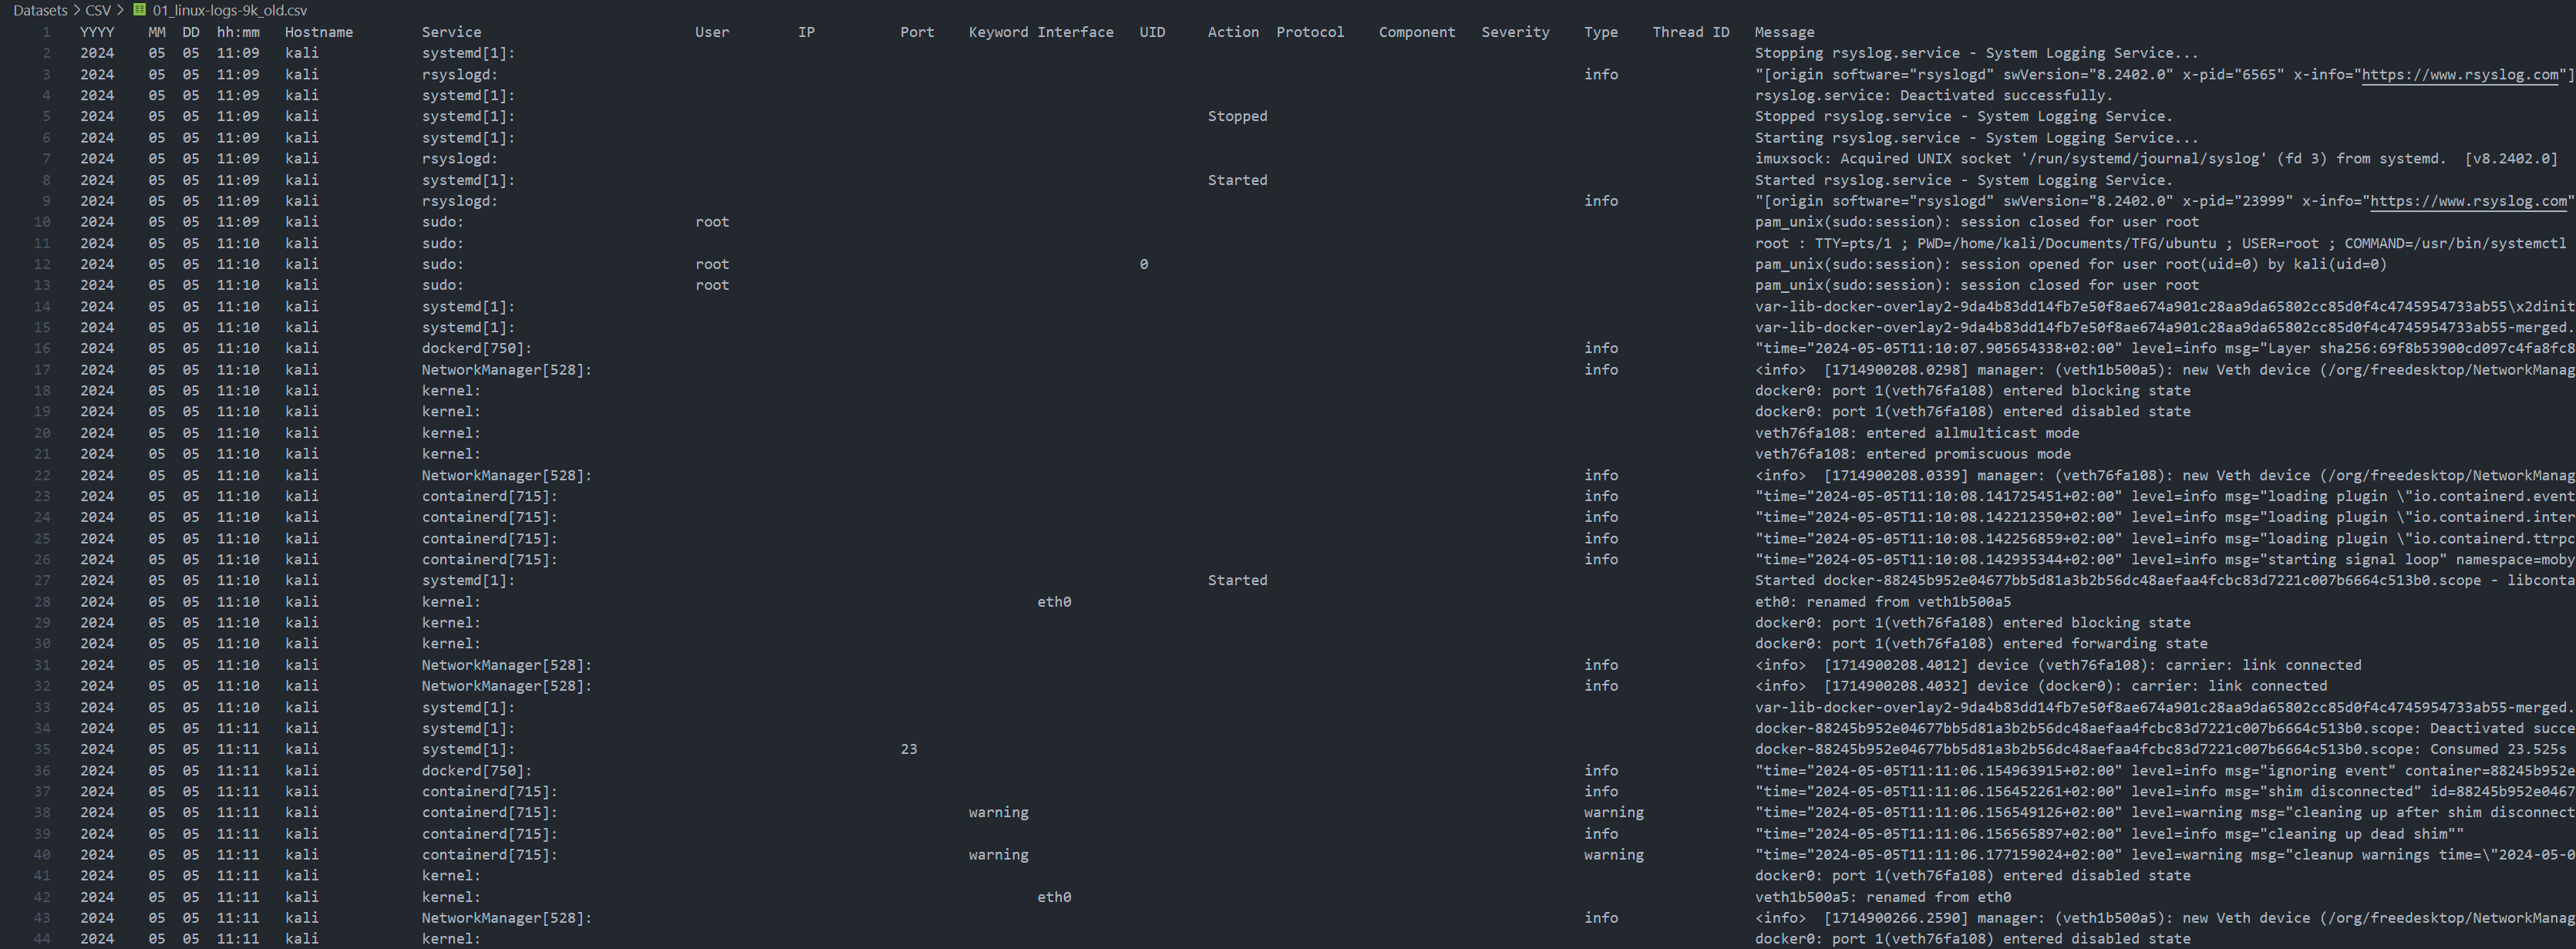
\includegraphics[width=1\linewidth]{imagenes/dataset-preprocesado.png}
    \caption{Estructura del \textit{dataset} tras fase de preprocesamiento}
    \label{fig:dataset-preprocesado}
\end{figure}

Tras este proceso de limpieza, preprocesamiento y extracción de características, los conjuntos de datos resultantes que serán usados para realizar el \textit{clustering} tienen las siguientes características:

\begin{table}[H]
\centering
\footnotesize
\begin{tabularx}{\textwidth}{|X|r|}
\hline
\rowcolor{graylight}\texttt{Nombre} & \texttt{Nº de eventos} \\ 
\hline
01\_linux-logs-9k.csv & 8890 \\ 
\hline
02\_linux-logs-2k.csv & 1546 \\ 
\hline
03\_HDFS-logs-20k.csv & 20000 \\ 
\hline
04\_BGL-logs-20k.csv & 20000 \\ 
\hline
05\_Synthetic-logs-5k.csv & 5000 \\
\hline
06\_auth-logs-20k.csv & 20000 \\
\hline
\end{tabularx}
\caption{Listado de conjuntos de datos preprocesados}
\label{tab:conjuntos-datos}
\end{table}

De los conjuntos de datos presentados en la Tabla \ref{tab:conjuntos-datos}, tres de ellos (03\_HDFS-logs-20k.csv, 04\_BGL-logs-20k.csv y 06\_auth-logs-20k.csv) son fragmentos de otros \textit{datasets} de mayor tamaño, que se han limitado a 20000 eventos. La decisión de no tomar los originales se ha sustentado en las limitaciones de cómputo disponibles para este Trabajo. Sin embargo, podría realizarse el mismo proceso utilizando sus versiones originales en caso de disponer de los recursos necesarios.

% ********************************************************************

\newpage

\section{Implementación del modelo}

Seguidamente, se llevó a cabo la implementación de distintos algoritmos de \textit{clustering} para clasificar los conjuntos de datos generados, y en base a los resultados obtenidos extraer potenciales vectores de ataque. A continuación se muestran las técnicas de vectorización de texto, reducción de dimensionalidad y extracción de características utilizadas, así como los pasos seguidos para implementar los algoritmos de agrupación.

\subsection{Técnicas utilizadas}

Se ha hecho uso de distintas técnicas que mejorasen la creación de agrupaciones de eventos para que estas fueran procesadas de forma más precisa, y otras técnicas para minimizar la cantidad de dimensiones y simplificar los datos sin perder la representatividad.

\subsubsection*{Técnicas de Vectorización de Texto}

La vectorización de texto se utiliza para transformar cada uno de los eventos de \textit{logs} en representaciones numéricas, de modo que estos puedan ser procesados por algoritmos de \gls{ML}. Para ello, se han utilizado las siguientes herramientas: \\

\textbf{\gls{TF}-\gls{IDF}}: (\textit{Term Frequency-Inverse Document Frequency}): convierte los \textit{logs} en una matriz de características \gls{TF}-\gls{IDF}. Como indica su acrónimo, puede desglosarse en dos partes con distinta funcionalidad:
\begin{itemize}
    \item \textbf{\gls{TF}} (\textit{Term Frequency}): en primer lugar, este mide la frecuencia de cada una de las palabras existentes en una línea y posteriormente las vectoriza, convirtiéndolas en un conjunto de números que representan la frecuencia de cada palabra en dicho documento \footnotemark. \\
    \item \textbf{\gls{IDF}} (\textit{Inverse Document Frequency}) \label{IDF}: en segundo lugar, se reduce la escala de las palabras que aparecen con mayor frecuencia en el conjunto de documentos o \textit{corpus}, y que por consiguiente son más discriminatorias con respecto a las demás palabras. Esto ayuda a resaltar aquellas palabras que son más únicas para cada \textit{dataset} de eventos de Linux. \\
\end{itemize}

\footnotetext{Cuando se habla de documentos en este contexto, nos referimos a una línea o conjunto de líneas del \textit{dataset}.}

A efectos matemáticos, según Ho Chung et. al \cite{tf-idf} se interpreta como el producto de las dos medidas, \gls{TF} e \gls{IDF}. Su valor puede calcularse de varias formas:

Por un lado, \textbf{\gls{TF}}, representado como tf(t, d), se suele usar la \textit{frecuencia bruta} del término t en el \textit{dataset} d, es decir, el nº de veces que una palabra o término t aparece en d. Denotando la frecuencia bruta de t por f(t,d), la función tf será tf(t, d) = f(t,d). También se pueden utilizar otras alternativas como las frecuencias booleanas, escalada logarítmicamente o la normalizada. 

\newpage

Esta última se calcula por el cociente de la frecuencia bruta entre la frecuencia máxima de alguna palabra (t) en el documento:

\begin{equation}
    \text{tf}(t, d) = \frac{f(t, d)}{\max\{f(t', d) : t' \in d\}}
\end{equation}

Por otro lado, \textbf{\gls{IDF}} mide si la palabra es común o no en el conjunto de \textit{corpus}. Se obtiene por medio del cociente del nº total de \textit{datasets} entre el número de \textit{datasets} que contienen la palabra, y se toma el logaritmo de dicho cociente:

\begin{equation}
    \text{idf}(t, D) = \log \left( \frac{|D|}{|\{d \in D : t \in d\}|} \right)
\end{equation}

donde:

\begin{itemize}
    \item $|D|$: cardinalidad de D, o número de \textit{datasets} en el conjunto. \\
    \item $|\{d \in D : t \in d\}|$: número de \textit{datasets} donde aparece la palabra o término t. Si no está en la colección se producirá una división-por-cero. Por lo tanto, es común ajustar esta fórmula a $1 + |\{d \in D : t \in d\}|$.
\end{itemize}

Por último, en cuanto a la base de la función \textit{log} no es relevante con respecto al resultado final obtenido. Por tanto, \gls{TF}-\gls{IDF} se calcula de la siguiente forma:

\begin{equation}
    \text{tfidf}(t, d, D) = \text{tf}(t, d) \times \text{idf}(t, D)
\end{equation}

La combinación de estos permite por tanto la vectorización de los \textit{logs} y al mismo tiempo la extracción de sus características. De cara a su uso en el \textit{notebook}, se han importado de la librería Sci-kit Learn (\ref{scikit}):

\begin{center}
    \begin{mdframed}
    \scriptsize
            \begin{minted}{javascript}
from sklearn.feature_extraction.text import TfidfVectorizer
            \end{minted}
    \end{mdframed}
\end{center}

La segunda técnica utilizada ha sido \textbf{Count-Vectorizer} \cite{scikit_count_vectorizer}. Esta herramienta se utiliza para transformar un \textit{dataset} de texto en una matriz numérica de recuentos de palabras.

A diferencia de \gls{TF}-\gls{IDF}, Count-Vectorizer simplemente cuenta la frecuencia de aparición de cada término en el documento, sin considerar la frecuencia inversa de los documentos. Esta es útil cuando se desea obtener una representación simple y directa de la frecuencia de los términos.

Su proceso puede describirse de la siguiente manera:

\begin{enumerate}
    \item Primero, se construye un vocabulario con todos los términos únicos presentes en el \textit{corpus}.
    \item Luego, se cuenta la frecuencia de aparición de cada término en cada línea, creando así una matriz en la que las filas representan líneas y las columnas representan los términos del vocabulario.
    \item Cada entrada en la matriz corresponde al número de veces que un término aparece en una línea específica.
\end{enumerate}

Este método es más sencillo y rápido de computar en comparación con \gls{TF}-\gls{IDF}, pero no proporciona la misma capacidad para diferenciar términos comunes y poco comunes en el conjunto de documentos. En el \textit{notebook}, se ha importado y utilizado de la librería Sci-kit Learn (\ref{scikit}) de la siguiente manera:

\begin{center}
    \begin{mdframed}
    \scriptsize
            \begin{minted}{javascript}
from sklearn.feature_extraction.text import CountVectorizer
            \end{minted}
    \end{mdframed}
\end{center}

De cara a futuras mejoras sería interesante utilizar otras alternativas como Word2Vec que aprende asociaciones de palabras a partir de grandes cantidades de datos en texto plano, y \gls{BERT}, o su versión adaptada a detección de anomalías de seguridad como \gls{BERT}-log \cite{guo2021logbert}.

\vspace{-2mm}

\subsubsection*{Técnicas de Reducción de Dimensionalidad}

La reducción de dimensionalidad en los \textit{corpus} de \textit{logs} ha implicado transformar datos complejos en una representación más simple y manejable, sin perder mucha información importante. Para lograr esto, se han utilizado tres técnicas distintas.

En primer lugar, \textbf{\gls{PCA}} (\textit{Principal Component Analysis}) \cite{Jolliffe2016PCA} transforma los datos a un nuevo sistema de coordenadas donde las mayores varianzas de los datos se proyectan en las primeras coordenadas. Esto permite reducir la dimensionalidad del \textit{corpus} de \textit{logs} manteniendo la mayor cantidad de varianza posible. Esta técnica es escalable a conjuntos de datos de un mayor tamaño, pero puede no capturar adecuadamente las complejas relaciones no lineales presentes en los \textit{logs} de eventos de seguridad, lo que puede afectar la precisión en la detección de patrones de ataque. 

Para utilizarla en el \textit{notebook}, se realiza el siguiente \textit{import}:

\begin{center}
    \begin{mdframed}
    \scriptsize
            \begin{minted}{javascript}
from sklearn.decomposition import PCA
            \end{minted}
    \end{mdframed}
\end{center}

En segundo lugar, \textbf{\gls{t-SNE}} (\textit{t-distributed Stochastic Neighbor Embedding}) \cite{Maaten2008tSNE}, convierte similitudes entre datos en alta dimensión en probabilidades conjuntas y minimiza la divergencia de Kullback-Leibler entre estas probabilidades en el espacio de baja dimensión. Esta es particularmente efectiva para la agrupación de eventos de \textit{logs}, ya que puede capturar relaciones no lineales y resaltar estructuras de \textit{clusters} que son críticas para la identificación de vectores de ataque. Sin embargo, \gls{t-SNE} puede ser computacionalmente costoso y no escalar bien con conjuntos de datos muy grandes, lo que podría limitar su aplicabilidad en escenarios con grandes volúmenes de datos de \textit{logs}. Se importa de la siguiente forma:

\begin{center}
    \begin{mdframed}
    \scriptsize
            \begin{minted}{javascript}
from sklearn.manifold import TSNE
            \end{minted}
    \end{mdframed}
\end{center}

Por último, \textbf{\gls{UMAP}} (\textit{Uniform Manifold Approximation and Projection}) \cite{McInnes2018UMAP} está basada en la teoría de grafos y la topología algebraica, por lo que preserva tanto la estructura local como global de los datos. \gls{UMAP} puede manejar grandes conjuntos de datos de manera eficiente y mantener la integridad de las relaciones tanto locales como globales. Esto facilita la detección de patrones complejos y anómalos en los \textit{logs} con relativa rapidez pero, en consecuencia, solamente es útil para un número de vecinos pequeño. Para hacer uso de esta, primero es necesario instalar la dependencia de \verb|umap-learn| y luego hacer el \textit{import}:

\begin{center}
    \begin{mdframed}
    \scriptsize
            \begin{minted}{javascript}
!pip install umap-learn
import umap.umap_ as umap
            \end{minted}
    \end{mdframed}
\end{center}

A través de todas las técnicas que han sido mencionadas, se tratará de mejorar el tratamiento de los \textit{dataset} y así obtener unos mejores resultados. Algunas de ellas serán combinadas y se analizará su rendimiento por medio de comparativas.

\subsection{Desarrollo del \textit{clustering}}

Una vez aplicadas las técnicas mencionadas anteriormente tanto para la vectorización de texto como para la reducción de la dimensionalidad, se ha llevado a cabo la implementación de los algoritmos de \textit{clustering} escogidos en el capítulo anterior. En el caso del \textit{clustering} jerárquico, se han utilizado tanto el algoritmo \gls{HC}, como la variante aglometariva: \gls{AHC}. A continuación se detalla el procedimiento seguido para cada uno de ellos.

Con el propósito de ir validando e ir haciendo un primer análisis sobre los resultados obtenidos, se ha ido imprimiendo un conjunto de gráficas, correspondientes a cada una de las combinaciones entre técnicas y algoritmos de \textit{clustering}, de modo que se estimara visualmente qué combinación respondía mejor frente a este tipo de de \textit{corpus}.


En esta sección, se mostrará el proceso para el tratamiento del conjunto de datos generado manualmente, es decir: \textit{01\_linux-logs-9k.csv}. En el caso de los demás \textit{datasets} se ha seguido estrictamente el mismo procedimiento. Por lo que en el próximo capítulo se analizarán y compararán los resultados obtenidos.

\subsubsection*{Implementación de K-means}

En primer lugar, para K-means se ha realizado la estimación del número óptimo de \textit{clusters} asociado al parámetro \textit{k} por medio del Algoritmo del Codo\footnotemark, mencionado en el capítulo cuarto \ref{fig:metodo-codo}. En la Figura \ref{fig:codo-manual} se muestran resultados obtenidos para el \textit{dataset} \textit{01\_linux-logs-9k.csv}.

Como se observa, pueden diferenciarse ligeramente tres codos. El primero de ellos en torno a \textit{k=5}, el segundo alrededor de \textit{k=10} y el último próximo a \textit{k=16}. Con el fin de verificar cual de estos valores es el más óptimo, se ha utilizado \textit{Silhouette Score} en el rango [2,31].

\newpage

\begin{figure}[H]
    \centering
    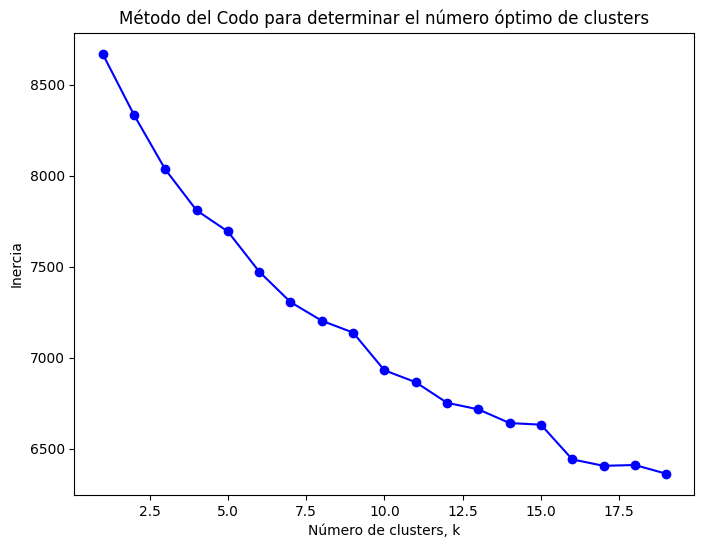
\includegraphics[width=0.95\linewidth]{imagenes/algoritmo-codo.png}
    \caption{Aplicación del Algoritmo del Codo sobre \textit{dataset} generado manualmente}
    \label{fig:codo-manual}
\end{figure}

\footnotetext{En la Figura \ref{fig:codo-manual} el eje \textit{y} está sociado a la Inercia, que es la suma de las distancias cuadradas de cada punto al centro de su \textit{cluster} más cercano.}


\begin{figure}[H]
    \centering
    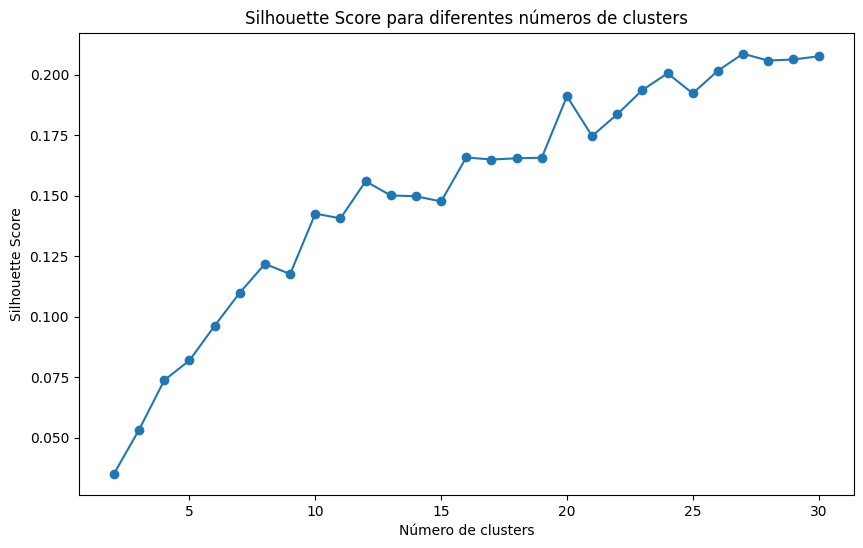
\includegraphics[width=0.95\linewidth]{imagenes/kmeans-silhouette.png}
    \caption{Cálculo del valor \textit{k} óptimo mediante Silhouette Score}
    \label{fig:kmeans-silhouette-optimo}
\end{figure}

\newpage

En base a los resultados visibles en la Figura \ref{fig:kmeans-silhouette-optimo}, no se observa ningún pico especialmente significativo salvo uno cercano a \textit{k=10}. Esto se debe a la heterogeneidad de los \textit{logs}, incluso aquellos asociados a ataques de fuerza bruta. Si el rango utilizado para aplicar \textit{Silhouette Score} aumentara, se ampliaría la cantidad de \textit{clusters}, pero lo más conveniente es seleccionar un número realista, por tanto se fijará \textit{k=10}.

Ahora se debe de llevar a cabo la inicialización del algoritmo utilizando 10 \textit{clusters} y un valor fijo para la semilla (en este caso 42), que será utilizada posteriormente para poder comparar todos los resultados obtenidos. Seguidamente se aplicará el algoritmo al \textit{dataset X}, de modo que se guarden todas las etiqutetas de \textit{cluster} asignadas a cada punto en \textit{kmeans\_labels}. 

\begin{center}
    \begin{mdframed}
    \footnotesize
            \begin{minted}{rust}
kmeans = KMeans(n_clusters=10, random_state=42)
kmeans_labels = kmeans.fit_predict(X)
            \end{minted}
    \end{mdframed}
\end{center}


Por último se añadirá al \gls{DF} una columna adicional que identificará la etiqueta de \textit{cluster} que le corresponda y se extraerán las características más representativas de cada uno de estos diez \textit{clusters}, de modo que pueda visualizarse posteriormente.


\begin{center}
    \begin{mdframed}
    \footnotesize
            \begin{minted}{rust}
data['kmeans_cluster'] = kmeans_labels
kmeans_cluster_terms = np.array([extract_cluster_terms(kmeans_labels, 
features, X.toarray())[i] for i in range(10)])
            \end{minted}
    \end{mdframed}
\end{center}

\subsubsection*{Implementación de \gls{DBSCAN}}

Para el caso de \gls{DBSCAN}, no se especifica directamente el número de \textit{clusters}, sino que se calcula en base a los parámetros \textit{eps} y \textit{min\_samples}. Tras realizar pruebas prácticas para ver qué valores respondían mejor, se han establecido los siguientes:

\[eps = 0.5, min\_samples = 5\]

\begin{center}
    \begin{mdframed}
    \footnotesize
            \begin{minted}{rust}
dbscan = DBSCAN(eps=0.5, min_samples=5)
dbscan_labels = dbscan.fit_predict(X)
            \end{minted}
    \end{mdframed}
\end{center}

Tras inicializar el algoritmo con los valores especificados, y a continuación aplicarlo al \textit{dataset}, se procede a añadir al \textit{dataframe} la nueva eiquetas y extraer las características.

\begin{center}
    \begin{mdframed}
    \footnotesize
            \begin{minted}{rust}
data['dbscan_cluster'] = dbscan_labels
dbscan_cluster_terms = extract_cluster_terms(dbscan_labels, features, 
X.toarray())
            \end{minted}
    \end{mdframed}
\end{center}

\newpage

\subsubsection*{Implementación de \gls{AHC} y \gls{HC}}

Para los algoritmos de \textit{clustering} jerárquico y aglomerativo, se ha optado por emplear el método de enlace \textit{ward}, que minimiza la suma de diferencias cuadradas dentro de todos los \textit{clusters}. Este método es menos susceptible a ruido y \textit{outliers} en comparación con otros métodos de enlace como el completo o el simple. Este utiliza la siguiente fórmula para calcular la distancia entre dos \textit{clusters} \(A\) y \(B\):

\[
    D(A,B) = \sqrt{\frac{|A| \times |B|}{|A| + |B|} \times ||\text{centroide}_A - \text{centroide}_B||^2}
\]

Después de calcular las distancias utilizando el método de enlace \textit{ward}, el siguiente paso es aplicar la función \textit{linkage} para construir la jerarquía de agrupaciones y luego usar \textit{fcluster} para formar los \textit{clusters}. De esta forma, será posible visualizar los dendogramas generados para poder hacer el análisis.

\begin{center}
    \begin{mdframed}
    \footnotesize
            \begin{minted}{rust}
linked = linkage(X.toarray(), method='ward') 
hierarchical_labels = fcluster(linked, 10, criterion='maxclust')
            \end{minted}
    \end{mdframed}
\end{center}

Una vez etiquetados los \textit{clusters}, se deben asignar estas etiquetas a los datos originales, de modo que puedan identificarse características comunes dentro de cada \textit{cluster}.

\begin{center}
    \begin{mdframed}
    \footnotesize
            \begin{minted}{rust}
data['hierarchical_cluster'] = hierarchical_labels
hierarchical_cluster_terms = extract_cluster_terms(hierarchical_labels, 
features, X.toarray())
            \end{minted}
    \end{mdframed}
\end{center}

En el caso del \textit{clustering} aglomerativo es similar al jerárquico pero con un enfoque más directo en la combinación progresiva de \textit{clusters} hasta alcanzar el número deseado de agrupaciones. Este método tenderá a dar mejores resultados con los \textit{datasets} con mayor volumen de datos, como se demostrará en el próximo capítulo.

\begin{center}
    \begin{mdframed}
    \footnotesize
            \begin{minted}{rust}
agglomerative_clustering = AgglomerativeClustering(n_clusters=9)
agglomerative_labels = agglomerative_clustering.fit_predict(X.toarray())
            \end{minted}
    \end{mdframed}
\end{center}

Finalmente, los resultados del \textit{clustering} aglomerativo se asignan a los datos, y se extraen términos representativos para cada \textit{cluster}.

\begin{center}
    \begin{mdframed}
    \footnotesize
            \begin{minted}{rust}
data['agglomerative_cluster'] = agglomerative_labels
agglomerative_cluster_terms = extract_cluster_terms(agglomerative_labels, 
features, X.toarray())
            \end{minted}
    \end{mdframed}
\end{center}

% ********************************************************************

\newpage

\section{Selección de métricas de evaluación}

El análisis del \textit{clustering} en el contexto de la detección de patrones de ataque en \textit{logs} requiere unas métricas específicas que reflejen la calidad de la agrupación más que la precisión de clasificación. Por este motivo, métricas comunes en otros contextos de aprendizaje supervisado como RECALL, PRECISION, o F1 Score no son aplicables aquí, ya que presuponen la existencia de etiquetas verdaderas previas, lo cual no se alinea con la naturaleza no supervisada del \textit{clustering} \cite{Rousseeuw1987}.

\subsubsection*{Silhouette Score}

El coeficiente de silueta mide cuán bien un objeto está emparejado a su propio \textit{cluster} comparado con otros clusters. Este coeficiente varía de -1 a 1, donde valores cercanos a 1 indican una asignación adecuada del objeto a su \textit{cluster}. La fórmula del coeficiente de silueta es:

\begin{equation}
    s = \frac{b - a}{\max(a, b)}
\end{equation}

donde \(a\) es la distancia media dentro del \textit{cluster} y \(b\) es la menor distancia media a cualquier otro cluster del que el objeto no es miembro.

Esta métrica viene implementada en \texttt{Python} a través dela librería \texttt{scikit-learn} (\ref{scikit}). Para ello, se utiliza el siguiente bloque de código:

\begin{center}
    \begin{mdframed}
    \scriptsize
            \begin{minted}{javascript}
from sklearn.metrics import silhouette_score
            \end{minted}
    \end{mdframed}
\end{center}

\subsubsection*{Índice de Davies-Bouldin}

El índice de Davies-Bouldin \cite{DaviesBouldin1979} es una métrica que evalúa la separación entre \textit{clusters}. Valores más bajos de este índice indican que los \textit{clusters} están bien separados y son compactos. La fórmula para calcular el índice de Davies-Bouldin \cite{petrovic2006comparison} es la siguiente:

\begin{equation}
    DB = \frac{1}{n} \sum_{i=1}^{n} \max_{j \neq i} \left( \frac{\sigma_i + \sigma_j}{d(c_i, c_j)} \right)
\end{equation}

donde \(\sigma\) es la dispersión dentro del \textit{cluster} y \(d(c_i, c_j)\) es la distancia entre los centroides de los clusters \(i\) y \(j\).

\vspace{2mm}

Al igual que la anterior, esta métrica viene implementada en \texttt{Python} por medio de \texttt{scikit-learn}. Puede importarse con:

\begin{center}
    \begin{mdframed}
    \scriptsize
            \begin{minted}{javascript}
from sklearn.metrics import davies_bouldin_score
            \end{minted}
    \end{mdframed}
\end{center}

\newpage

\subsubsection*{Índice de Calinski-Harabasz}

Por último, el índice de Calinski-Harabasz \cite{CalinskiHarabasz1974} compara la dispersión entre los \textit{clusters} con la dispersión existente dentro de los \textit{clusters}. Valores más altos indican una mejor definición de los \textit{clusters}. La fórmula para el índice de Calinski-Harabasz es:

\begin{equation}
    CH = \frac{SSB / (k - 1)}{SSW / (n - k)}
\end{equation}

donde \(SSB\) es la suma de cuadrados entre los \textit{clusters}, \(SSW\) es la suma de cuadrados dentro de los \textit{clusters}, \(k\) es el número de \textit{clusters}, y \(n\) es el número de puntos.

Para importar esta métrica se usa una vez más la implementación proporcionada por \texttt{scikit-learn}:

\begin{center}
    \begin{mdframed}
    \scriptsize
            \begin{minted}{javascript}
from sklearn.metrics import calinski_harabasz_score
            \end{minted}
    \end{mdframed}
\end{center}

Para calcular en el \textit{notebook} las distintas métricas utilizadas, se he hecho uso del siguiente fragmento de código:

\begin{center}
    \begin{mdframed}
    \scriptsize
            \begin{minted}{javascript}
metrics = {
    'Método de Clustering': ['K-Means', 'DBSCAN', 'Clustering Jerárquico', 
    'Clustering Jerárquico Aglomerativo'],
    'Silhouette Score': [
        silhouette_score(X, kmeans_labels),
        silhouette_score(X, dbscan_labels) if len(set(dbscan_labels)) > 1 
        else "No aplicable",
        silhouette_score(X, hierarchical_labels),
        silhouette_score(X, agglomerative_labels)
    ],
    'Índice Davies-Bouldin': [
        davies_bouldin_score(X.toarray(), kmeans_labels),
        davies_bouldin_score(X.toarray(), dbscan_labels) 
        if len(set(dbscan_labels)) > 1 else "No aplicable",
        davies_bouldin_score(X.toarray(), hierarchical_labels),
        davies_bouldin_score(X.toarray(), agglomerative_labels)
    ],
    'Índice Calinski-Harabasz': [
        calinski_harabasz_score(X.toarray(), kmeans_labels),
        calinski_harabasz_score(X.toarray(), dbscan_labels) 
        if len(set(dbscan_labels)) > 1 else "No aplicable",
        calinski_harabasz_score(X.toarray(), hierarchical_labels),
        calinski_harabasz_score(X.toarray(), agglomerative_labels)
    ]
}
            \end{minted}
    \end{mdframed}
\end{center}

\newpage


Por tanto, los valores que pueden tomar los resultados utilizando las métricas mencionadas pueden corresponden con los de la Tabla \ref{tab:intervalos_metricas}.

\begin{table}[H]
\centering
\footnotesize
\begin{tabularx}{\textwidth}{|X|r|r|}
\hline
\rowcolor{graylight}\texttt{Métrica} & \texttt{Mínimo} & \texttt{Máximo} \\ 
\hline
Coeficiente de Silueta & -1 & 1 \\ 
\hline
Índice de Davies-Bouldin & 0 & $\infty$ \\
\hline
Índice de Calinski-Harabasz & 0 & $\infty$ \\
\hline
\end{tabularx}
\caption{Intervalos de oscilación para las métricas de evaluación del \textit{clustering}}
\label{tab:intervalos_metricas}
\end{table}

\subsubsection*{Extracción de términos principales}

Además de llevar a cabo el análisis del \textit{clustering} por medio de las tres métricas mencionadas anteriormente, se han implementado varias funciones que permitan extraer las palabras clave asoaciadas a cada \textit{cluster} y graficarlas junto a la imagen donde se visualizan los puntos. 

\begin{center}
    \begin{mdframed}
    \scriptsize
            \begin{minted}{python}
# Función para extraer palabras clave por cluster
def extract_cluster_terms(labels, features, X, n_words=10):
    unique_labels = np.unique(labels)
    cluster_terms = {}
    for label in unique_labels:
        if label != -1:  # Excluir clusters marcados como ruido por DBSCAN
            indices = np.where(labels == label)[0]
            if len(indices) > 0:
                cluster_data = X[indices]
                centroid = np.mean(cluster_data, axis=0).flatten()
                top_indices = np.argsort(-centroid)[:n_words]
                cluster_terms[label] = [features[i] for i in top_indices]
    return cluster_terms
            \end{minted}
    \end{mdframed}
\end{center}

De esta forma, es posible entender cómo cada algoritmo está agrupando los distintos conjuntos de eventos, y por consiguiente identificar aquella/s agrupaciones asociadas a posibles riesgos de seguridad en el sistema operativo. 

\begin{center}
    \begin{mdframed}
    \scriptsize
            \begin{minted}{python}
# Función para pintar y mostrar términos de cluster
def plot_and_print_clusters(X_pca, labels, title, cluster_terms, n_clusters=None):
    plt.figure(figsize=(10, 8))
    scatter = plt.scatter(X_pca[:, 0], X_pca[:, 1], c=labels, cmap='tab10', 
    marker='o', edgecolor='black')
    plt.title(title)
    plt.colorbar(scatter, ticks=np.unique(labels))
    plt.show()
    if n_clusters:
        for i in range(n_clusters):
            print(f"Cluster {i}: {', '.join(cluster_terms[i])}")
    else:
        for label, terms in cluster_terms.items():
            print(f"Cluster {label}: {', '.join(terms)}")
            \end{minted}
    \end{mdframed}
\end{center}


\chapter{Análisis de resultados}

En este capítulo se hará un estudio de los resultados obtenidos tras aplicar \textit{clustering} a los distintos \textit{datasets} de logs, y en base a las métricas utilizadas y las gráficas obtenidas medir cuales de ellos responden mejor de cara a la detección de potenciales vectores de ataque.

% ********************************************************************

\section{Evaluación de la efectividad de los modelos}

Con el objetivo de evaluar cómo han respondido cada uno de los \textit{datasets} anteriores, se va a proceder a analizar los valores calculados a través de las métricas de Silhouette Score, el índice de Davies-Bouldin y el índice de Calinski-Harabasz. Además, se hará un análisis de las gráficas en las que se ha mapeado cada \textit{cluster} a los conjuntos de eventos y palabras contenidas en ellos.

Comenzando con el \textit{dataset} generado manualmente, \texttt{01\_linux-logs-9k.csv}, según las métricas este ha respondido mejor aparentemente con \gls{DBSCAN} usando ambas técnicas de vectorización. Sin embargo, esto se debe a que el número de \textit{clusters} ha sido muy elevado. Observando la gráfica de la Figura \ref{fig:k-means-tf-idf-t-sne}, puede observarse un resultado ampliamente mejor para el caso de K-means con \gls{TF}-\gls{IDF} y la técnica de reducción de dimensionalidad \gls{t-SNE}. En dicho ejemplo el vector de ataque se encuentra en el tercer \textit{cluster}, cuyas palabras asociadas son las siguientes:

\begin{center}
    \begin{mdframed}
    \footnotesize
            \begin{minted}{javascript}
Cluster 3: port, 172, 17, ssh2, password, failed, invalid, anonymous, 
user, root
            \end{minted}
    \end{mdframed}
\end{center}


En este ejemplo hay cierto margen de mejora, ya que se está agrupando en el \textit{cluster} 8 otro conjunto asociado aun vector de ataque que debería haberse unificado con el anterior. Lo mismo sucede con el \textit{cluster} 2, aunque este en menor medida.

\begin{center}
    \begin{mdframed}
    \footnotesize
            \begin{minted}{javascript}
Cluster 8: euid, ruser, logname, rhost, tty, ssh, authentication, uid, 
172, failure
Cluster 2: pass, unknown, check, auth, sshd, pam_unix, user, device, devel
            \end{minted}
    \end{mdframed}
\end{center}
\newpage

Igualmente, el resto de \textit{clusters} no presentan ninguna palabra que esté potencialmente asociada a ningún tipo de ataque, por lo que puede concluirse un resultado bastante positivo. El vector de ataque detectado en este conjunto de datos está directamente relacionado con un intento de inicio de sesión fallido a través del servicio de \gls{SSH} por parte de varios usuarios en reiteradas ocasiones: \texttt{root} y \texttt{anonymous}, lo cual podría estar directamente relacionado con un ataque del tipo \textit{Malformed Packet} para descubrir usuarios comunes listados en un diccionario, o bien con un ataque por diccionario para esos dos usuarios en concreto.

\begin{figure}[H]
    \centering
    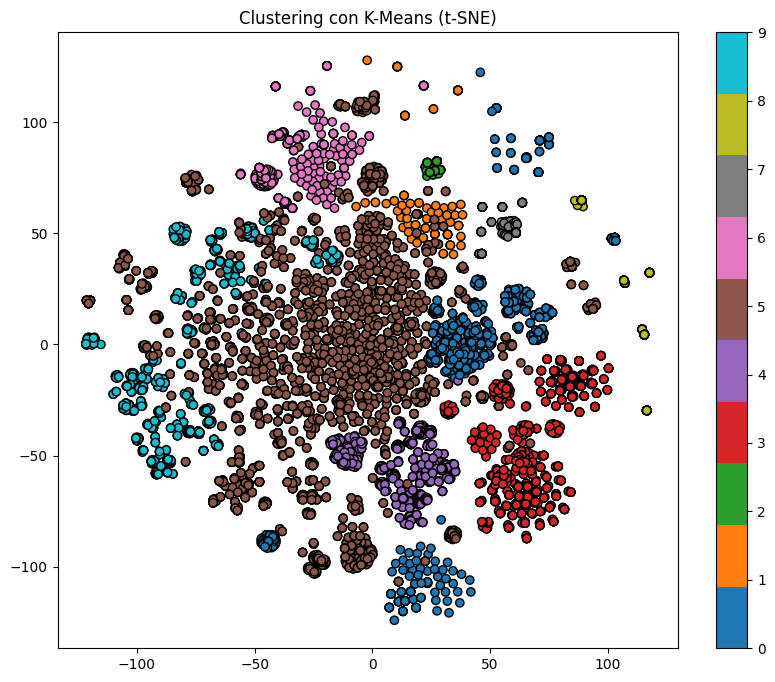
\includegraphics[width=0.7\linewidth]{imagenes/k-means-tf-idf-t-sne.png}
    \caption{Clustering con K-Means utilizando \gls{TF}-\gls{IDF} y \gls{t-SNE}}
    \label{fig:k-means-tf-idf-t-sne}
\end{figure}

\vspace{-3mm}

El resto de \textit{clusters}, como se ha indicado anteriormente, no contienen ninguna palabra que pueda estar asociada algún ataque:


\begin{mdframed}
\scriptsize
\begin{minted}{javascript}
Cluster 0: main, 09, 08, dnd, x11, received, events, debian, host, 47
Cluster 1: retries, ignoring, max, pam, sshd, service, devices, device, devel
Cluster 4: containerd, 05, info, io, msg, 2024, time, level, 02, v1
Cluster 5: service, target, pipewire, agent, device, entered, socket, starting
Cluster 6: session, uid, pam_unix, cron, root, user, opened, closed, sudo, lightdm
Cluster 7: supervising, processes, threads, users, 10, 12, 13, 11, 14, 15
Cluster 9: service, successfully, org, bus, pid, uid, deactivated, 1000, dbus
\end{minted}
\end{mdframed}

Comparando el resultado obtenido con \gls{TF}-\gls{IDF} en K-means y a continuación, con \textit{Count Vectorizer} en \gls{AHC} (Figura \ref{fig:k-means-count-vectorizer-t-sne}), se observa una ligera mejora, ya que la amplia mayoría de \textit{logs} asociados a ataques se agrupan en el \textit{cluster} dos, y el resto en el quinto y el séptimo.

\begin{mdframed}
\scriptsize
\begin{minted}{javascript}
Cluster 2: port, 172, 17, ssh2, password, failed, invalid, anonymous, user, root
Cluster 5: euid, ruser, logname, rhost, tty, ssh, authentication, uid, 172, 
failure
Cluster 7: pass, unknown, check, auth, sshd, pam_unix, user, device, devel,
failure
\end{minted}
\end{mdframed}

\begin{figure}[H]
    \centering
    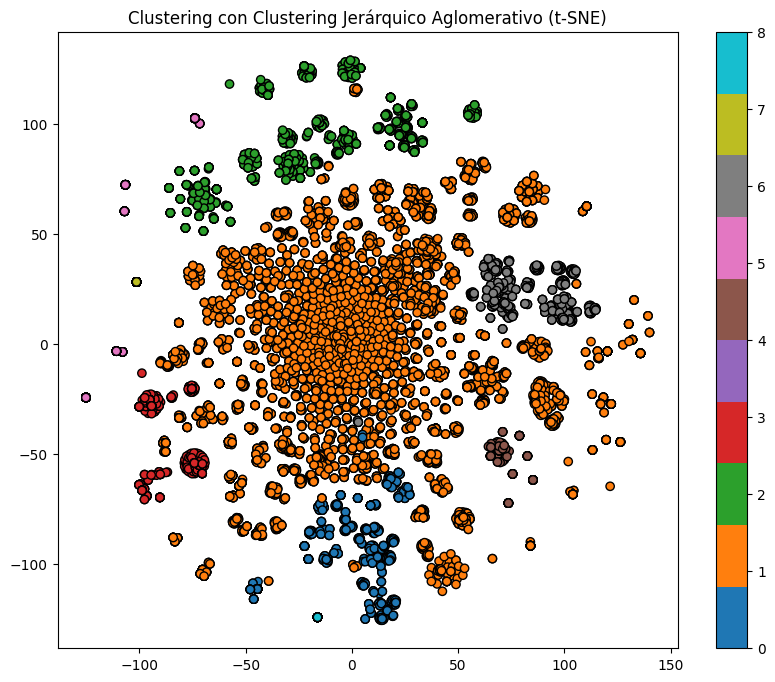
\includegraphics[width=0.7\linewidth]{imagenes/AHC-count-vectorizer-t-sne.png}
    \caption{Clustering con \gls{AHC} utilizando \textit{Count Vectorizer} y \gls{t-SNE}}
    \label{fig:k-means-count-vectorizer-t-sne}
\end{figure}

El hecho de que \gls{DBSCAN} haya tenido buenos resultados con \textit{Silhouette Score} y al mismo tiempo unos muy bajos en las otras dos métricas como se muestra en la Figura \ref{fig:dataset_01}, se debe a la gran cantidad de \textit{clusters} que tiene, de modo que reajustando sus parámetros podría mejorar el resultado en estas últimas. No obstante, se tendrá en cuenta este resultado para ver qué comportamiento presenta este algoritmo de \textit{clustering} en los demás conjuntos de datos.

\begin{figure}[H]
    \centering
    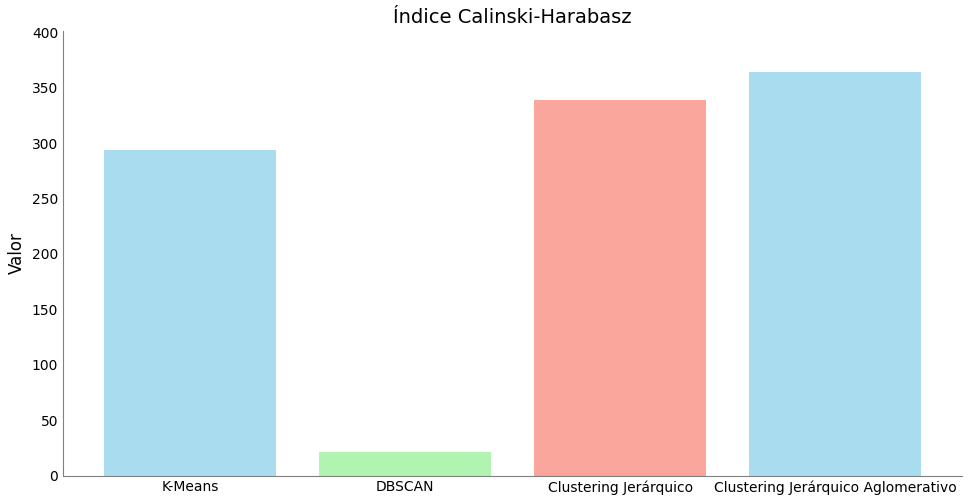
\includegraphics[width=0.8\linewidth]{imagenes/dataset_01_calinski.png}
    \caption{Resultados obtenidos en \textit{dataset} manual según índice de Calinski-Harabasz}
    \label{fig:dataset_01}
\end{figure}

En el caso del segundo conjunto de datos: \texttt{02\_linux-logs-2k.csv}, el cual contiene también eventos generados por \textit{syslog} en una máquina Linux del año 2016, se incluyen principalmente intentos de inicio de sesión fallidos. Al aplicar los cuatro algoritmos de \textit{clustering}, se han obtenido algunos resultados de interés. \\

Para el algoritmo \textit{K-means} se aplicó el Algoritmo del Codo, y se obtuvo un valor de codo cercano a k=4 tal y como se muestra en la Figura \ref{fig:metodo-codo-dataset-02}. En este caso el resultado es claro, por lo tanto ha sido necesario aproximar de nuevo el valor de \textit{k} por medio de Silhouette Score.

\begin{figure}[H]
    \centering
    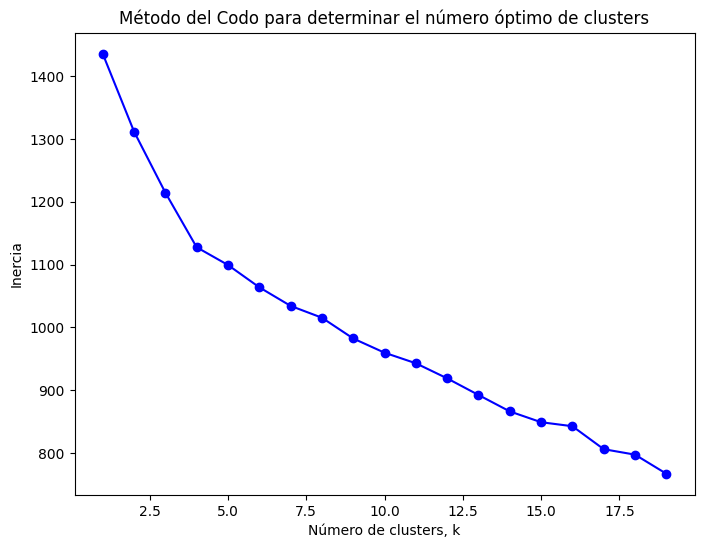
\includegraphics[width=0.7\linewidth]{imagenes/metodo-codo-dataset_02.png}
    \caption{Cálculo del método del codo para el \textit{dataset} \texttt{02\_linux-logs-2k.csv}}
    \label{fig:metodo-codo-dataset-02}
\end{figure}

\vspace{-2mm}

Utilizando ambas técnicas de reducción de dimensionalidad se obtienen unos resultados muy similares. Los \textit{logs} asociados a eventos críticos de seguridad se han podido agrupar en un mismo \textit{cluster}: el número uno.

\begin{figure}[H]
    \centering   
    \begin{minipage}{0.4\textwidth}
        \centering
        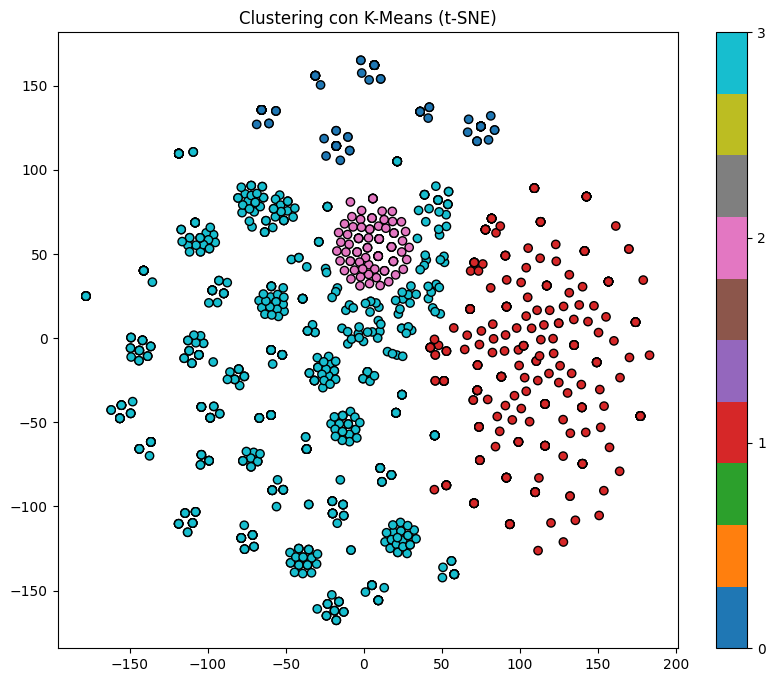
\includegraphics[width=\linewidth]{imagenes/dataset_02_k-means_t_sne_count_vectorizer.png}
        \caption{Clustering de \textit{Linux\_2k} con K-means utilizando \gls{TF}-\gls{IDF} y \gls{t-SNE}}
        \label{fig:dataset_02_k-means_tsne_tf_idf}
    \end{minipage}
    \hspace{0.1\textwidth}
    \begin{minipage}{0.4\textwidth}
        \centering
        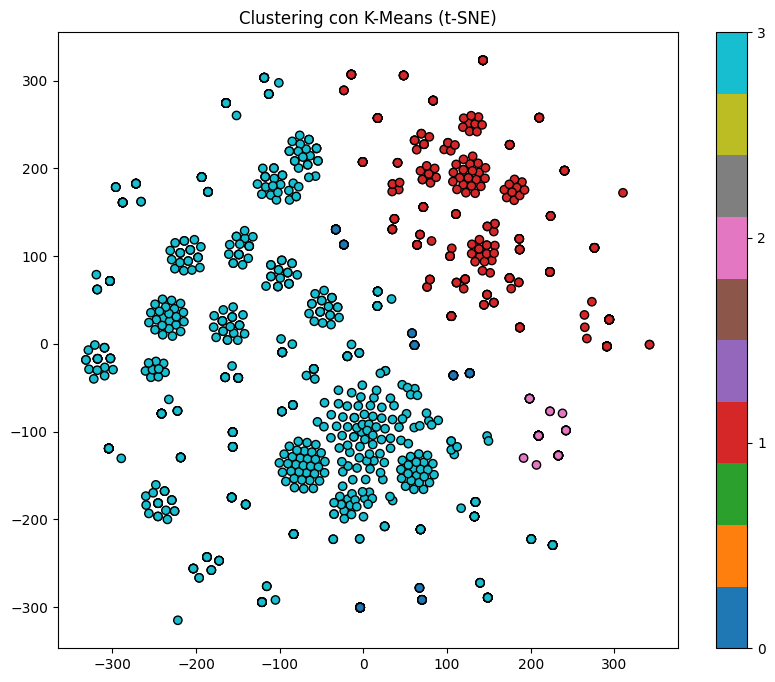
\includegraphics[width=\linewidth]{imagenes/dataset_02_k-means_tsne_tf_idf.png}
        \caption{Clustering de \textit{Linux\_2k} con K-means utilizando \textit{Count-Vectorizer} y \gls{t-SNE}}
        \label{fig:dataset_02_k-means_tsne_count_vectorizer}
    \end{minipage}
\end{figure}

En la Figura \ref{fig:dataset_02_k-means_tsne_tf_idf} se agrupan bajo el \textit{cluster} uno, al igual que en la Figura \ref{fig:dataset_02_k-means_tsne_count_vectorizer}. Además su contenido es equivalente:

\begin{mdframed}
\scriptsize
\begin{minted}{javascript}
Cluster 1: ruser, rhost, euid, logname, tty, failure, nodevssh, authentication, 
uid, root
\end{minted}
\end{mdframed}

Para realizar una comparativa con \textit{datasets} de eventos distintos a los de \textit{syslog} en Linux, se ha seleccionado el conjunto de datos asociado a un fragmento de 20000 líneas de \gls{HDFS}, generado en el año 2008. Los resultados obtenidos distan bastante con los anteriores, en primer lugar debido a que ha aumentado significativamente el volumen de datos \textit{clusterizados}, y en segundo lugar por la información recopilada por estos \textit{logs}, por tanto se presentan anomalías distintas, tal y como se muestra en la Figura \ref{fig:hdfs-ahc-t-sne} en el caso del algoritmo \gls{AHC}. Al aplicar el método del codo, se ha obtenido un valor óptimo de \textit{clusters} con \textit{k=13}.

\begin{figure}[H]
    \centering
    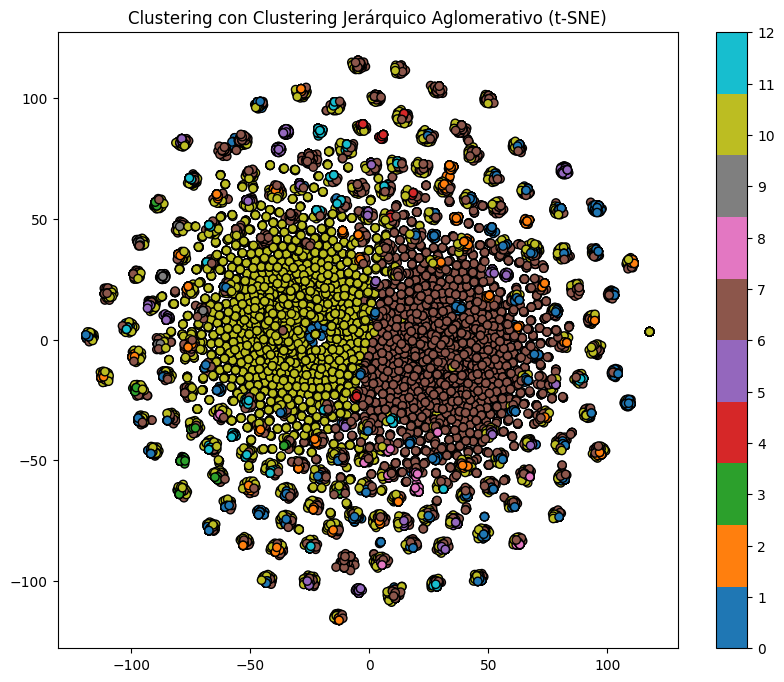
\includegraphics[width=0.8\linewidth]{imagenes/dataset_03_AHC_tf_idf.png}
    \caption{Clustering de \gls{HDFS} con \gls{AHC} utilizando \gls{TF}-\gls{IDF} y \gls{t-SNE}}
    \label{fig:hdfs-ahc-t-sne}
\end{figure}

En la Figura \ref{fig:hdfs-ahc-t-sne}, los principales \textit{clusters} son el siete y el diez. Cada uno de ellos hace referencia a operaciones críticas sobre grandes bloques de datos, como finalizar una transferencia. Sin embargo, no se aprecia ninguna operación que llegue a resultar de utilidad para detectar algún tipo de acción indeseada, por lo que se demuestra una vez más la vital importancia de que los \textit{logs} registren la información de la manera más clara posible en lenguaje natural, de modo que pueda ser clasificada de forma óptima por modelos de inteligencia artificial. Los \textit{logs} de \gls{HDFS} utilizan una terminología muy específica y ambigüa, que tendría que ser mapeada para poder facilitar al modelo su proceso de razonamiento y que pueda otorgar buenos resultados.

\begin{mdframed}
\scriptsize
\begin{minted}{javascript}
Cluster 7: terminating, block, updated, added, size, 67108864, 50010, 10, 251,250
Cluster 10: blk_, terminating, block, updated, added, 67108864, size, 50010, 10,25
\end{minted}
\end{mdframed}

En cuarto lugar, para \gls{BGL}, que se trata de un conjunto de datos del supercomputador de \gls{IBM} como se ha explicado en capítulos anteriores, se ha calculado un valor óptimo de \textit{k=4} \textit{clusters}. Este valor, al igual que en los ejemplos anteriores, se ha calculado a partir de aplicar el Algoritmo del Codo. En este caso se han agrupado en el cluster cero (azul) \textit{cluster} los eventos asociados a errores del \textit{Kernel}, como se puede observar en la Figura \ref{fig:dataset_04_umap}. 

\begin{figure}[H]
    \centering
    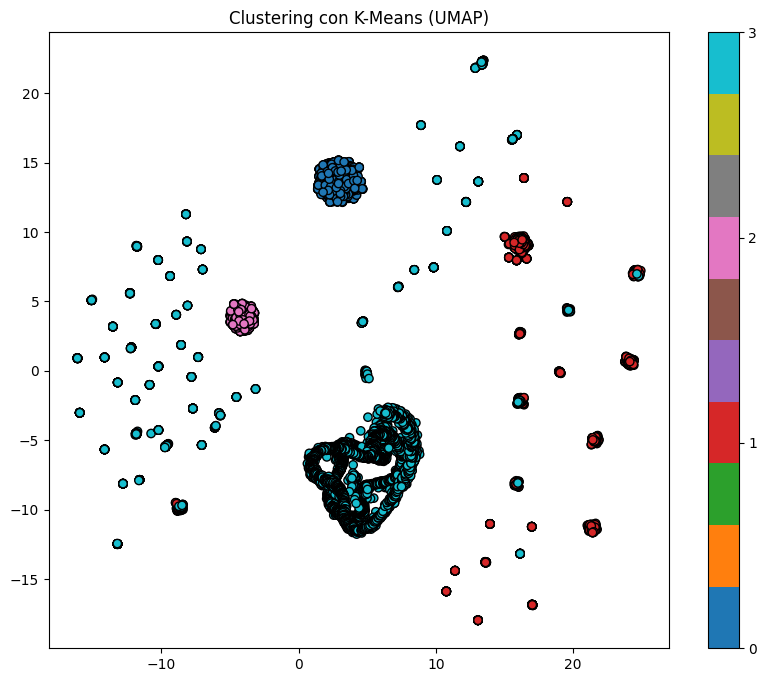
\includegraphics[width=0.6\linewidth]{imagenes/dataset_04_k-means-umap.png}
    \caption{Clustering de \gls{BGL} con K-means utilizando \gls{TF}-\gls{IDF} y \gls{UMAP}}
    \label{fig:dataset_04_umap}
\end{figure}

Se han obtenido unos resultados prácticamente equivalentes para el caso de los algoritmos de \textit{clustering} jerárquico y su variante aglomerativa. De los cuatro \textit{clusters}, se dividen varios tipos de alertas. Por un lado, en el grupo cero aquellas relacionados con errores del \textit{kernel} y la memoria caché. En el caso del \textit{cluster} uno, se agrupan problemas relacionados con excepciones y aliniamiento. Esto es positivo, ya que no simplemente se agrupan alertas en uno solo, sino que se fusionan en base a la tipología del error que ocasiona el evento.


\begin{mdframed}
\scriptsize
\begin{minted}{javascript}
Cluster 0: cache, instruction, parity, corrected, error, info, kernel, 35737, 
35717, 35716
Cluster 1: hummer, exceptions, double, alignment, kernel, info, 182, 162, 141, 142
Cluster 2: message, ciostream, control, socket, prefix, stream, read, 96, 116, 172
Cluster 3: info, core, generating, kernel, mask, ce, sym, 0x08, detected, ddr
\end{minted}
\end{mdframed}

En quinto lugar, el \textit{dataset} que ha sido generado de forma sintética, estaba formado de forma intencionada únicamente por alertas de seguridad asociadas a ataques de distinto ámbito. Si se obtienen unos buenos resultados, sería indicativo de que los algoritmos de \textit{clustering} responden de una forma adecuada cuando los conjuntos de datos de \textit{logs} son robustos, es decir, contienen eventos con una información completa y clara.

Los mejores resultados se han obtenido a través de la reducción de dimensionalidad con \textit{Count Vectorizer} y la vectorización de texto con \gls{t-SNE}. Como se observa en la Figura \ref{fig:dataset_05_count_vectorizer_t_sne}, se agrupan anomalías principalmente en los \textit{clusters} tres, uno y ocho. Su contenido difiere principalmente por los usuarios involucrados en el proceso de autenticación a un servidor \gls{SSH}. 

\begin{figure}[H]
    \centering
    \includegraphics[width=0.7\linewidth]{imagenes/dataset-sintético-t-sne-count-vectorizer.png}
    \caption{Clustering de \gls{AHC} en \textit{dataset} sintético con \textit{Count Vectorizer} y \gls{t-SNE}}
    \label{fig:dataset_05_count_vectorizer_t_sne}
\end{figure}

\vspace{-1mm}

En el siguiente fragmento de código se muestra el conjunto de palabras asociado a cada \textit{cluster}. El primero de ellos hace referencia a varios elementos como la desconexión de un suario y un intento de sesión fallida. El segundo (\textit{cluster 3}, se asocia con un \textit{login} inválido a causa de un usuario inexistente y otros exitosos pero de riesgo debido a que están relacionados con usuarios con permisos de administrador. Por último, el \textit{cluster} ocho contiene palabras relacionadas con un posible ataque de fuerza bruta que ha alcanzado un máximo de intentos de autenticación para un usuario \texttt{admin}. \\

\begin{mdframed}
\scriptsize
\begin{minted}{javascript}
Cluster 1: port, 168, 192, ssh2, failed, transfer, completed, user, disconnected
Cluster 3: logged, 168, 192, test, admin, guest, root, invalid_user, 51, 101
Cluster 8: exceeded, authentication, attempts, preauth, ssh2, port, 192, 168, 
test, admin
\end{minted}
\end{mdframed}


Una vez más, las métricas de Índice de Davies-Bouldin \cite{DaviesBouldin1979} e Índice de Calinski-Harabasz \cite{CalinskiHarabasz1974} otorgan una mayor puntuación a los algoritmos K-means, \gls{HC} y \gls{AHC}, mientras que \textit{Silhouette Score} da la valoración más positiva a \gls{DBSCAN}.

Finalmente, para el conjunto de datos \texttt{06\_auth-logs-20k.csv}, se ha calculado de nuevo mediante el Algoritmo del Codo el valor de \textit{k} para utilizarlo en los algoritmos jerárquicos y K-means, obteniendo un valor de 12. El tamaño original de este era de 47000 eventos de seguridad, sin embargo debido a las limitaciones de computación ha sido necesario tomar un fragmento de 20000.

Los resultados obtenidos han sido, en comparación con los \textit{datasets} generados tanto de forma manual como sintética, significativamente peores, tal y como puede observarse en la Figura \ref{fig:dataset_06}. 

\newpage

Esto se debe principalmente a que los eventos capturados en este fichero provienen del fichero \texttt{auth.log}, que únicamente almacena logs a sociados a intentos de inicio de sesión fallidos. Es por ello, que sería interesante tratar de otro modo el \textit{corpus} para que se realizara el \textit{clustering} en base a los usuarios que han llevado a cabo el proceso de autenticación.

\begin{figure}[H]
    \centering
    \includegraphics[width=0.675\linewidth]{imagenes/dataset_06_count_vectorizer_t-sne.png}
    \caption{Clustering de \gls{HC} en \texttt{06\_auth-logs-20k.csv} con \textit{Count Vectorizer} y \gls{t-SNE}}
    \label{fig:dataset_06}
\end{figure}

\vspace{-4mm}

Todas las gráficas anteriores que muestran los resultados de un análisis de \textit{clustering} después de aplicar alguna técnica de reducción de dimensionalidad se representan por los siguientes ejes:
\begin{itemize}
    \item \texttt{Eje X} (horizontal): Corresponde a la primera componente principal, que captura la dirección de máxima varianza de los datos, mostrando dónde los datos varían más.
    \item \texttt{Eje Y} (vertical): Corresponde a la segunda componente principal, que captura la siguiente dirección de máxima varianza, perpendicular a la primera. \\
\end{itemize}


En conclusión, los algoritmos de \textit{clustering} que mejor han respondido ante estos conjuntos de datos han sido, por amplia diferencia K-means y los algoritmos jerárquicos \gls{HC} y \gls{AHC}. En cuanto a la técnica de vectorización de texto que mejores prestaciones ha tenido en base a las métricas utilizadas ha sido \textit{Count Vectorizer}. Por último, la técnica de reducción de dimensionalidad que ha permitido graficar de forma más óptima los conjuntos de \textit{logs} ha sido \gls{t-SNE}. 

En la Figura \ref{fig:resultados-dataset-manual} pueden visualizarse los resultados obtenidos para el \textit{dataset} generado manualmente (\texttt{01\_linux-logs-9k.csv}) aplicando los distintos algoritmos de \textit{clustering} en base a las técnicas utilizadas para vectorización de texto y reducción de dimensionalidad. Además, en la Tabla \ref{tab:metricas} pueden consultarse los valores obtenidos en base a las tres métricas utilizadas y clasificados por algoritmo utilizado y técnica de vectorización de texto.

\newpage
  
\noindent \hspace{-11mm}
\begin{minipage}{\linewidth}
        \begin{figure}[H]
            \centering
            \includegraphics[width=1.2\linewidth, keepaspectratio]{imagenes/graficas-dataset-manual.png}
            \caption{Resultados del \textit{clustering} obtenidos en el \textit{Dataset} manual}
            \label{fig:resultados-dataset-manual}
        \end{figure}
\end{minipage}

\newpage
\thispagestyle{empty}

\begin{landscape}
    \noindent\hspace*{-3.1cm}
    \footnotesize
    \begin{tabularx}{2.1\textwidth}{|l|>{\hsize=1\hsize}X|X|X|X|X|X|X|X|X|}
    \rowcolor{graylight}
        \hline
        \multicolumn{2}{|l|}{\texttt{Métrica Utilizada}} & \multicolumn{4}{c|}{\texttt{TF-IDF}} & \multicolumn{4}{c|}{\texttt{CountVectorizer}} \\ \hline
        \texttt{Dataset} & \texttt{Número Eventos} & \texttt{K-means} & \texttt{DBSCAN} & \texttt{HC} & \texttt{AHC} & \texttt{K-means} & \texttt{DBSCAN} & \texttt{HC} & \texttt{AHC} \\ \hline
        \rowcolor{graylight} \multicolumn{10}{|c|}{\texttt{Silhouette Score}} \\ \hline
        \texttt{01\_linux-logs-9k.csv} & 8890 & 0,142565 & \textbf{0,327076} & 0,148059 & 0,138362 & 0,045752 & 0,223888 & 0,056558 & 0,047342    \\ \hline
        \texttt{02\_linux-logs-2k.csv} & 1546 & 0,186831 & \textbf{0,856451} & 0,186831 & 0,186831 & 0,120715 & 0,834370 & 0,120715 & 0,120715    \\ \hline
        \texttt{03\_HDFS-logs-20k.csv} & 20000 & 0,055194 & -0,01371 & 0,020737 & 0,018550 & \textbf{0,129202} & -0,10574 & 0,026898 & 0,024624   \\ \hline
        \texttt{04\_BGL-logs-20k.csv} & 20000 & 0,367028 & 0,476697 & 0,363458 & 0,363458 & 0,596589 & 0,345334 & \textbf{0,582639} & \textbf{0,582639}   \\ \hline
        \texttt{05\_Synthetic-logs-5k.csv} & 5000 & 0,183675 & \textbf{0,327810} & 0,168854 & 0,177956 & 0,166143 & 0,254842 & 0,172808 & 0,153171    \\ \hline
        \texttt{06\_auth-logs-20k.csv} & 20000 & 0,337545 & 0,661056 & 0,342969 & 0,342969 & 0,351366 & \textbf{0,645813} & 0,277735 & 0,277735  \\ \hline
        \rowcolor{graylight} \multicolumn{10}{|c|}{\texttt{Indice de Davies-Bouldin}} \\ \hline
        \texttt{01\_linux-logs-9k.csv} & 8890 & \textbf{3,160860} & 1,101850 & 2,215990 & 2,427580 & 2,543825 & 1,217092 & 1,697760 & 1,813962    \\ \hline
        \texttt{02\_linux-logs-2k.csv} & 1546 & \textbf{2,042738} & 1,040805 & \textbf{2,042738} & \textbf{2,042738} & 1,638323 & 0,840527 & 1,638323 & 1,638323   \\ \hline
        \texttt{03\_HDFS-logs-20k.csv} & 20000 & 3,914300 & 1,052135 & 5,081278 & \textbf{5,365123} & 2,195493 & 1,426535 & 3,877497 & 4,802849   \\ \hline
        \texttt{04\_BGL-logs-20k.csv} & 20000 & 1,830761 & 0,952598 & \textbf{1,883499} & \textbf{1,883499} & 0,728352 & 0,854809 & 0,759906 & 0,759906   \\ \hline
        \texttt{05\_Synthetic-logs-5k.csv} & 5000 & \textbf{2,471757} & 1,028901 & 2,254009 & 2,359428 & 1,789288 & 1,127338 & 1,673542 & 1,722449   \\ \hline
        \texttt{06\_auth-logs-20k.csv} & 20000 & \textbf{2,067445} & 1,035235 & 1,589178 & 1,589178 & 1,695114 & 0,982265 & 1,317203 & 1,317203   \\ \hline
        \rowcolor{graylight} \multicolumn{10}{|c|}{\texttt{Indice de Calinski-Harabaz}} \\ \hline
        \texttt{01\_linux-logs-9k.csv} & 8890 & 247,64400 & 24,20370 & 254,66300 & 267,61000 & 293,662881 & 21,363775 & 338,759653 & \textbf{364,631418}  \\ \hline
        \texttt{02\_linux-logs-2k.csv} & 1546 & 140,494849 & 156,210995 & 140,494849 & 140,494849 & 205,211041 & \textbf{235,150142} & 205,211041 & 205,211041   \\ \hline
        \texttt{03\_HDFS-logs-20k.csv} & 20000 & 254,81996 & 170,938375 & 173,080575 & 180,749527 & 1303,516335 & 10,251355 & 607,210643 & \textbf{664,011968}    \\ \hline
        \texttt{04\_BGL-logs-20k.csv} & 20000 & 4263,557621 & 159,093892 & 4176,9412 & 4176,9412 & \textbf{18712,75285} & 182,430667 & 17821,29833 & 17821,29833   \\ \hline
        \texttt{05\_Synthetic-logs-5k.csv} & 5000 & 249,890189 & 58,079644 & 255,864348 & 263,576459 & 530,687883 & 60,799303 & 554,721452 & \textbf{565,499024}  \\ \hline
        \texttt{06\_auth-logs-20k.csv} & 20000 & 1443,017509 & 112,332262 & 1431,08245 & 1431,08245 & \textbf{3297,852755} & 148,411853 & 2295,506274 & 2295,506274    \\ \hline
    \end{tabularx}
    \begin{table}[H]
        \centering
        \caption{Métricas obtenidas en los distintos conjuntos de datos}
        \label{tab:metricas}
    \end{table}
\end{landscape}

\newpage

% ********************************************************************

\section[Estudios previos para la detección de amenazas]{Análisis comparativo. Estudios previos para la detección de amenazas}

En la misma línea que este Trabajo de Fin de Grado, a lo largo de estos últimos años han emergido numerosas propuestas para la detección proactiva de actividades maliciosas por medio de técnicas que apliquen de un modo u otro inteligencia artificial. A lo largo de esta sección se abordarán las principales alternativas publicadas en distintas fuentes institucionales como \textit{Google Scholar}, \textit{Scopus} o \textit{Science Direct}. \\

% ********************************************************************

\subsubsection*{Primer caso de Estudio}

Comenzando por el artículo publicado por Kayhan et. al \cite{KAYHAN2023113928}, se propone el uso de \gls{UHAC} (\textit{Unsupervised hunting of anomalous commands}), que precisamente sigue el enfoque de detectar anomalías a través de conjuntos de datos no etiquetados en \gls{SIEM}s mediante \textit{clustering}. En concreto, hace uso de \gls{TF}-\gls{IDF} para la creación de la matriz de características y \gls{DBSCAN} para el \textit{clustering}. Además, emplea una función de pérdida personalizada que le permite manejar de forma adecuada los pesos binarios\footnotemark. Los comandos se van ordenando en base a su error de reconstrucción, de modo que los errores más altos son indicativo de una mayor probabilidad de la existencia de anomalías. 

\footnotetext{Pesos que indican la presencia (1) o ausencia (0) de características específicas en los comandos.}

En esta investigación, se hizo uso de \gls{OC-SVM} (\textit{One-Class Support Vector Machine}), que se trata de una técnica de clasificación empleada para la detección de anomalías, especialmente efectiva en contextos donde los datos etiquetados son escasos o inexistentes. Este construye un modelo a partir de un conjunto de datos no etiquetados, diferenciando entre patrones normales y aquellos que se consideran anomalías, mediante la maximización del margen de separación en un espacio de características transformado.

\subsubsection*{Segundo caso de Estudio}

En el \textit{paper} publicado por Tendikov et. al \cite{TENDIKOV2024102254}, se lleva a cabo una evaluación de la efectividad de distintos modelos de \gls{ML} con el propósito principal de detectar intrusiones en redes. Para ello, se levó a cabo una recopilación datos de máquinas virtuales Windows capturados por un \gls{SIEM}, más concretamente ataques web procedentes del \textit{dataset} CICIDS2017 \cite{sharafaldin2018toward}. En cuanto a las técnicas de \textit{clustering} utilizadas, se incluyen \textit{Random Forest} y K-means, así como técnicas de vectorización de texto como \gls{TF}-\gls{IDF} y de reducción de dimensionalidad como \gls{PCA} y \gls{t-SNE}. Por último, para medir los resultados obtenidos se hizo uso de la métrica F1 Score, mediante la cual se obtuvo un 0,97 utilizando \textit{Random Forest}.

\newpage

% ********************************************************************

\subsubsection*{Tercer caso de Estudio}
% https://link.springer.com/book/10.1007/978-3-030-74450-2 
En tercer lugar, en el libro de Skopik et. Al \cite{skopik2021smart}, se lleva a cabo una clasificación de los tipos de anomalías que pueden llegar a ser detectadas a través de algoritmos de \textit{clustering}. Entre estas destacan:

\begin{itemize}
\item \texttt{Outliers}\label{outliers}: también conocidos como valores atípicos, son líneas de registro individuales que no coinciden con ninguna de las plantillas existentes o son disímiles a todos los \textit{clusters} identificados que representan el comportamiento normal del sistema. Un ejemplo podría ser un mensaje de error en un archivo de registro que generalmente solo contiene mensajes informativos y de depuración. \\
\item \texttt{Anomalías de Frecuencia}: son eventos de registro que aparecen con una frecuencia inesperadamente alta o baja durante un intervalo de tiempo dado. Esto incluye casos donde los componentes dejan de registrar eventos o la detección de ataques que implican la ejecución de muchos eventos, como los escaneos de vulnerabilidades. \\
\item \texttt{Anomalías de Correlación}: eventos que se espera que ocurran en pares o grupos pero no lo hacen. Un claro ejemplo serían anomalías de coocurrencia y de implicación, es decir, aquellos eventos que deberían implicar la ocurrencia de otros. \\
\item \texttt{Anomalías de Tiempo entre Llegadas}: Causadas por intervalos de tiempo desviados entre la ocurrencia de \textit{logs}. Estas están relacionadas con las de correlación y pueden proporcionar capacidades de detección adicionales, por ejemplo, si un evento esperado no ocurre dentro de una ventana de tiempo específica. \\
\item \texttt{Anomalías de Secuencia}: son provocadas por eventos faltantes o adicionales, así como por órdenes desviadas en secuencias de eventos de registro que se esperan ocurran en ciertos patrones.
\end{itemize}

Estos tipos de anomalías pueden ser detectadas o apoyadas por técnicas de \textit{clustering} tanto estáticas como dinámicas, dependiendo del tipo específico de anomalía. Los \textit{outliers} pueden ser identificados mediante algoritmos de \textit{clustering} estático, mientras que las demás anomalías requieren técnicas de \textit{clustering} dinámico y análisis estadístico para detectar violaciones en las correlaciones esperadas.

% ********************************************************************

\subsubsection*{Cuarto caso de Estudio}
% https://ieeexplore.ieee.org/document/10306968
Otro caso digno de análisis es el del \textit{paper} publicado por Tharunika et. al \cite{10306968}, titulado \textit{Detection and Prevention of Advanced Persistent Threat (APT) Activities in Heterogeneous Networks using \gls{SIEM} and Deep Learning}. En este se comenta el uso de modelos de \gls{ML} y \gls{DL} para la detección y prevención de anomalías de red en \gls{SIEM}s. Para ello, se hace uso de la arquitectura de la Figura \ref{fig:architecture-diagram}.

\begin{figure}[H]
    \centering
    \includegraphics[width=1\linewidth]{imagenes/architecture-diagram-v3.png}
    \caption{Diagrama de la arquitectura propuesta por Tharunika et. al \cite{10306968}}
    \label{fig:architecture-diagram}
\end{figure}

Tal y como se puede observar, tras el proceso de recopilación del conjunto de datos, se lleva a cabo una fase de preprocesamiento en la que se eliminan \gls{NaN}s, líneas duplicadas y \textit{outliers} \ref{outliers}. A continuación se lleva a cabo el \textit{encoding} y la selección de características. Seguidamente, se hace uso de técnicas de reducción de la dimensionalidad como \gls{PCA} y \gls{SVD}. Se emplean además algoritmos de \textit{clustering} como \gls{SMOTE} o K-means. Finalmente se lleva a cabo la generación de modelos, más concretamente se utilizan los siguientes:

\begin{itemize}
    \item Modelos de \gls{ML}: \gls{KNN}, \gls{SVM}, \textit{Random Forest} y Árboles de decisión.
    \item Modelos de \gls{DL}: \gls{ANN} y \gls{LSTM}.
\end{itemize}

Por medio del uso de estos modelos, se trataba de detectar si un \textit{log} o conjunto de \textit{logs} estaban asociados a un ataque de tipo \gls{DDoS} o si eran benignos. Para evaluar los resultados obtenidos se hizo uso de cuatro métricas distintas. Estas métricas fueron: \textit{Precission}, \textit{Recall}, \textit{F1-Score} y \textit{Accuracy}. Según las tablas obtenidas se obtuvieron unos resultados muy positivos, lo cual demuestra de nuevo la importancia de llevar a cabo un buen preprocesamiento de los conjuntos de datos de \textit{logs}.

% ********************************************************************

\subsubsection*{Quinto caso de Estudio}
% https://ieeexplore.ieee.org/stamp/stamp.jsp?tp=&arnumber=9614848
En línea con los estudios previos, el trabajo realizado por Datta et al. \cite{9614848} en su artículo titulado \textit{Real-time Threat Detection in \gls{UEBA} using Unsupervised Learning Algorithms} se enfoca en la detección de amenazas en tiempo real mediante el uso de algoritmos de aprendizaje no supervisado en el análisis del comportamiento de usuarios y entidades (\gls{UEBA}). En este estudio, se comparan cuatro algoritmos de \textit{clustering} no supervisados para detectar amenazas internas de manera eficiente.

Para la reducción de dimensionalidad, se utilizó el \gls{PCA}, permitiendo reducir las características del conjunto de datos a las más relevantes. En cuanto a las técnicas de preprocesamiento incluyeron \textit{One-Hot Encoding} para transformar datos categóricos en formato binario, estandarización para ajustar los valores de los datos, y la eliminación de duplicados y valores atípicos y así mejorar la calidad del conjunto de datos.

\newpage

Los modelos de \textit{Machine Learning} utilizados fueron:
\begin{itemize}
    \item \texttt{K-Means} (\ref{k-means})
    \item \texttt{\gls{AHC}} (\ref{dbscan})
    \item \texttt{\gls{DBSCAN}} (\ref{AHC})
    \item \texttt{\gls{GMM} (\textit{Gaussian Mixture Model})}: este es un modelo probabilístico que asume la existencia de un número finito de distribuciones Gaussianas, cada una representando un cluster. \\
\end{itemize}

Para evaluar el rendimiento de los algoritmos utilizados, se emplearon las mismas métricas que se han empleado para este Trabajo de Fin de Grado, es decir, Silhouette Score, índice de Calinski-Harabasz e Índice de Davies-Bouldin. Los resultados obtenidos en esta investigación fueron los mostrados en la Tabla \ref{tab:ueba-results}.

\begin{table}[H]
\centering
\footnotesize
\begin{tabularx}{\textwidth}{|X|X|X|X|}
\hline
\rowcolor{graylight} \texttt{Modelo} & \texttt{Silhouette Score} & \texttt{Calinski-Harabasz} & \texttt{Davies-Bouldin} \\ \hline
K-Means & 0.2372 & 887.8355 & 1.2291 \\ \hline
Agglomerative Clustering & 0.2291 & 718.8155 & 1.4191 \\ \hline
DBSCAN & 0.3782 & 345.2103 & 2.2108 \\ \hline
Gaussian Mixture Model (GMM) & 0.0697 & 191.3066 & 2.4507 \\ \hline
\end{tabularx}
\caption{Resultados obtenidos por Datta et al. \cite{9614848} empleando algoritmos de \textit{clustering} para la detección de amenazas}
\label{tab:ueba-results}
\end{table}

De este estudio se concluye que los algoritmos K-Means y \textit{Agglomerative Clustering} fueron los más eficientes para la detección de amenazas internas. Una vez más, se prueba que funcionan los métodos de \textit{clustering} no supervisados de cara a la detección de comportamientos anómalos en entornos de ciberseguridad. \\

% https://www.frontiersin.org/articles/10.3389/fdata.2024.1375818/full
Otro artículo estrechamente relacionado con este, es el de Artioli et al. \cite{artioli2024comprehensive}, en el cual se lleva a cabo una investigación exhaustiva sobre algoritmos de \textit{clustering} tanto tradicionales como emergentes aplicados a la \gls{UEBA}. En este estudio, se abordan diferentes contextos de aplicación y se consideran múltiples escenarios de interacción usuario-entidad. 

Artioli et al. comparan quince algoritmos de \textit{clustering} en tres conjuntos de datos diferentes, en los que destaca principalmente el rendimiento prometedor de \gls{HDBSCAN} y \gls{DenMune} en el conjunto de datos de comportamiento \gls{CERT}, generando grupos con una densidad muy cercana al número de usuarios.


% ********************************************************************

\subsubsection*{Sexto caso de Estudio}

En contraste con los casos de estudio anteriores, se ha tenido en cuenta el desarrollo de un \gls{LLM} orientado a ciberseguridad llamado \texttt{0dai} \cite{Navarrete2024}. A lo largo del año 2023 y este 2024, ha ido optimizándose y mejorando su capacidad de resolución de actividades relacionadas con el \textit{hacking} ético y la ciberseguridad. 0dai, además del uso genérico de \gls{LLM}s como \texttt{ \gls{GPT}} \cite{10500411} o \texttt{\gls{Gemini}} \cite{imran2024google}, propone el uso de agentes capaces de llevar a cabo ejercicios de \textit{pentesting} en hasta 15 minutos.

A diferencia de otros \textit{large model languages}, este no solo evita las limitaciones convencionales de su uso para actividades relacionadas con el \textit{hacking}, sino que está mejorado para implementar \textit{scripts} que utilicen herramientas de seguridad comunes e incluso implementar \textit{malware}. 

Además, \texttt{0dai} ha ido adquirido diversas funcionalidades adicionales. Ahora permite la integración con \gls{IDS}s y \gls{EDR}s, herramientas directamente relacionadas con un \gls{SIEM}. También ofrece acceso a una \textit{\gls{API} key} que permite usar el modelo de forma más personalizada, y ha logrado la integración con más de 50 herramientas de ciberseguridad. 

La reciente actualización \texttt{0dai} v2.0 incluye un modelo con 50 mil millones de parámetros y un sistema de registro para el \gls{FS}. Entre las herramientas utilizadas por sus usuarios se encuentran la implementación de \textit{bypass} de \textit{Cloudflare}, la herramienta Auto-\gls{XSS} para detectar vulnerabilidades \gls{XSS}, y mejoras en herramientas de \gls{OSINT} para buscar contraseñas y datos en brechas de seguridad.

Más allá de la ética relacionada con el uso que se le puede dar a este tipo de soluciones tecnológicas, pueden surgir múltiples soluciones que hasta ahora no se habían llevado a cabo. En base a una reunión con su entonces director de tecnología Luis Javier Navarrete, el pasado 8 de junio, se comentó que una de estas soluciones sería la creación de \textit{datasets} sintéticos a partir de agentes preparados con una serie de instrucciones muy específicas, de modo que se formaran conjuntos de datos verdaderamente útiles para entrenar modelos capaces de detectar anomalías de seguridad en distintos sistemas como Linux. 

Sin embargo, podría ser de mayor utilidad cambiar el enfoque de la metodología utilizada para la detección de vectores de ataque en este tipo de sistemas, de modo que se prepararan conjuntos de datos completamente etiquetados y que contuvieran información adicional, como mapear para cada \textit{log} si existe algún tipo de riesgo o no, o asignarle un potencial tipo de ataque (p.e. \gls{DDoS} o fuerza bruta al \textit{login} de algún servicio).

% ********************************************************************

% https://www.researchgate.net/profile/Omar-Al-Sanjary/publication/343408460_Comparison_and_Detection_Analysis_of_Network_Traffic_Datasets_Using_K-Means_Clustering_Algorithm/links/5f9977a9299bf1b53e4bb7df/Comparison-and-Detection-Analysis-of-Network-Traffic-Datasets-Using-K-Means-Clustering-Algorithm.pdf

\section{Sinergias e integración con sistemas \gls{SIEM}}
% https://www.mdpi.com/2076-3417/13/11/6610 

En el contexto de la amenaza constante por parte de los cibercriminales y ciberterroristas, la integración de la \gls{IA} con sistemas \gls{SIEM} es crucial para la detectar de forma efectiva incidentes y dar respuesta a estos en el menor tiempo posible. Según Ban et al.\cite{bantao2023}, los \gls{SIEM}s modernos deben abordar con diversos problemas, como es el caso de la fatiga de alertas, que puede llegar a resolverse mediante el uso de técnicas avanzadas de \gls{ML} y visualización de datos en tiempo real.

\vspace{-2mm}

\subsection{Beneficios de la integración}

La integración con sistemas \gls{SIEM} ya está proporcionando múltiples beneficios que pueden ser ampliados, entre ellos destacan:

\begin{itemize}
    \item Centralización de datos: la consolidación de \textit{logs} y eventos de seguridad en una plataforma centralizada facilita su análisis y correlación a los analistas de seguridad.

    \item Automatización de respuestas: Los \gls{SIEM}s pueden incorporar capacidades de \gls{SOAR} para automatizar tareas de respuesta a incidentes, mejorando la eficiencia operativa. 
    
    \item Reducción de falsos positivos: utilizando algoritmos de aprendizaje no supervisado o supervisado, como \gls{IWSVM} (\textit{Instance-Weighted Support Vector Machine}), propuesto por Ban et al.\cite{bantao2023}\footnotemark, es posible filtrar alertas irrelevantes y priorizar incidentes críticos.  
\end{itemize}

\footnotetext{\gls{IWSVM} es una mejora del \gls{SVM} tradicional que asigna diferentes pesos a las instancias basándose en su importancia, mejorando el rendimiento en conjuntos de datos desbalanceados.}

\vspace{-2mm}

\subsection{Desafíos y soluciones}

Uno de los mayores desafíos en la gestión de eventos de seguridad actualmente es la cantidad abrumadora de alertas generadas diariamente. Como se menciona en el trabajo de Ban et al.\cite{bantao2023}, se propuso un marco de \gls{SIEM} de próxima generación que integra capacidades avanzadas de \gls{SOAR} y utiliza una estrategia de \gls{DAC} para mitigar el impacto de las alertas de baja calidad.

A pesar de la funcionalidad que ofrecen los \gls{SIEM}s, estos presentan un cuello de botella con respecto a la toma de determinadas decisiones. Actualmente, en muchos casos es necesario que un profesional determine manualmente si hay algún tipo de intento de intrusión maliciosa, si hay un falso positivo o si simplemente no hay actividad inusual. Por lo tanto, a pesar de que la intervención humana seguirá siendo necesaria, la automatización de múltiples tareas permitirá que lso analistas inviertan su tiempo únicamente en decisiones críticas e \gls{I+D}. \\

La integración propuesta en este Trabajo de Fin de Grado implica la adopción por parte de un \gls{SIEM} de técnicas de \gls{ML} y visualización avanzada de los datos, con el principal propósito de mejorar la detección y respuesta a incidentes de seguridad. Entre estas técnicas, se propone especialmente utilizar algoritmos de \textit{clustering} como K-means y \gls{AHC}, ya que permiten una clasificación mucho más precisa que otras como \gls{DBSCAN} según los resultados obtenidos.

De tal modo, se conseguirá una sinergia con sistemas \gls{SIEM} que permitirá no solo la centralización y correlación de datos, sino también la automatización de tareas propias de un analista, así como la reducción de falsos positivos. En conclusión, los \gls{SIEM}s han sido desarrollados para ayudar a los administradores, no a sustituir su trabajo, y a facilitar el diseño de políticas de seguridad y la gestión de eventos con la mayor celeridad posible, aumentando su efectividad frente métricas como el \gls{MTTD} y \gls{MTTR}.



\chapter{Conclusiones y trabajo futuro}

% ********************************************************************

\vspace{-5mm}

\section{Resumen de los logros obtenidos}

Tras llevar a cabo este Trabajo de investigación acerca del análisis de \textit{logs} de Linux por medio de algoritmos de \textit{clustering} para detectar potenciales vectores de ataque, y con la finalidad principal de integrar esta funcionalidad en \gls{SIEM}s para que estos mejoren los tiempos de respuesta, se han extraído las siguientes conclusiones:

\begin{itemize}
\item \texttt{Acerca de los \textit{logs} de Linux}: Los \textit{logs} de este sistema operativo son suficientemente ricos como para ser aprovechados en la detección de anomalías de distintos tipos. Se pueden identificar desde ataques remotos como fuerza bruta y denegación de servicio, hasta ataques a nivel del kernel o más bajo nivel. \\
\item \texttt{Acerca del preprocesamiento de \textit{logs}}: Esta es la parte más crucial del proceso. Lograr un dataset bien etiquetado mejora significativamente los resultados obtenidos. Sin embargo, también puede ser muy positivo el uso datasets no etiquetados como se ha llevado a cabo en este Trabajo. \\
\item \texttt{Acerca de los modelos de \gls{ML} utilizados}: Tras probar distintos algoritmos de \textit{clustering}, los mejores resultados se obtuvieron con \textit{k-means} y \textit{clustering} jerárquico. Aun así, sería conveniente probar otros algoritmos de aprendizaje automático como \gls{KNN}, \gls{SVM}, \textit{Random Forest}, \textit{Decision Tree}, entre otros. \\
\item \texttt{Acerca de la integración con \gls{SIEM}s}: Desde hace algunos años se ha comenzado a integrar estas técnicas, pero el proceso es lento. Es vital seguir investigando para reducir los tiempos de detección de amenazas y generación de respuestas verdaderamente eficaces.
\end{itemize}

Con estos logros se ha demostrado que el análisis de \textit{logs} de Linux mediante técnicas de \textit{clustering} es una herramienta potente para la detección de vectores de ataque, y su integración en \gls{SIEM}s es una vía prometedora para mejorar la ciberseguridad.

% ********************************************************************

\newpage

\section{La importancia del Software Libre}

El software libre juega un papel fundamental en el avance de la tecnología y la ciencia abierta. Permite el acceso libre y gratuito a información, herramientas y recursos que pueden ser utilizados y modificados por cualquier persona. En el contexto de la ciberseguridad, el software libre ofrece varias ventajas cruciales.

La transparencia es una de estas ventajas. Al ser accesible para todos, cualquier persona puede revisar el código fuente y asegurarse de que no contiene vulnerabilidades o puertas traseras. Esto aumenta la confianza en la seguridad y fiabilidad del software utilizado. Un ejemplo reciente es el de la biblioteca de compresión \texttt{xz} \cite{goodin2024xzbackdoor}, donde se descubrió una puerta trasera en su código. La comunidad de código abierto reaccionó rápidamente, identificando y parcheando la vulnerabilidad, demostrando así la eficacia del escrutinio público en la detección y corrección de fallos de seguridad.

Otra ventaja es la colaboración. El software libre facilita la coordinación entre investigadores, desarrolladores y profesionales de la seguridad, quienes pueden contribuir con mejoras y nuevas funcionalidades. Esta colaboración abierta fomenta un entorno de innovación constante y rápida evolución tecnológica. Desde el ámbito personal, ha sido de gran utilidad para entender qué metodologías seguir para el proceso de análisis de \textit{logs}. Un ejemplo de esta colaboración en el ámbito de la Universidad de Granada, es la labor realizada por la Oficina de Software Libre \cite{oslugr}, que promueve la enseñanza a jóvenes en estas tecnologías de libre acceso.

El software libre también fomenta la innovación. Cualquiera puede tomar un proyecto existente y modificarlo para adaptarlo a nuevas necesidades o desarrollar nuevas soluciones. Esto hace que las herramientas evolucionen rápidamente y se adapten a los cambios y desafíos del entorno tecnológico. La comunidad de Linux es el principal ejemplo de que la innovación viene de la colaboración altruista, ya que es algo que beneficia a todos. En esta línea, muchas grandes empresas \cite{recluit2024opensource} están empezando a contribuir económicamente para que se invierta en herramientas \textit{opensource}.

La accesibilidad es otro aspecto importante. El software libre hace que las herramientas de seguridad estén disponibles para una audiencia más amplia, incluyendo organizaciones pequeñas y países en desarrollo que no pueden permitirse costosas licencias de software propietario. Esto democratiza el acceso a tecnologías avanzadas y promueve la equidad en el ámbito tecnológico.

En resumen, el software libre y la ciencia abierta permiten que los resultados de la investigación sean compartidos y verificados por la comunidad científica global. Esto no solo mejora la calidad y la fiabilidad de la investigación, sino que también acelera el desarrollo de nuevas tecnologías y soluciones, beneficiando a toda la sociedad.

% ********************************************************************

\newpage

\section{Líneas de investigación y desarrollo futuras (I\texttt{+}D)}

\vspace{4mm}

Para seguir avanzando en el campo de la detección de vectores de ataque a través del análisis de \textit{logs}, se identifican varias líneas de \gls{I+D} que resultan prometedoras y necesarias.

Primero, es fundamental ampliar la variedad de vectores de ataque utilizados en las simulaciones realizadas. Estos pueden incluir desbordamiento de buffer (\textit{buffer overflow}), condiciones de carrera (\textit{race conditions}), inyecciones \gls{SQL}, \gls{XSS} o ejecución de \textit{scripts} con firma desconocida, entre otros. Entender y detectar una gama más amplia de vectores de ataque permitirá crear sistemas de defensa más robustos y adaptativos.

En segundo lugar, se debe evaluar el uso de otros algoritmos de aprendizaje automático (\gls{ML}) como \gls{KNN}, \textit{Random Forest}, \gls{RRNN}s y \gls{SVM}. Probar estos algoritmos en diferentes contextos y con distintos tipos de datos permitirá identificar cuáles son más efectivos para la detección de anomalías en los \textit{logs}.

Además, diversificar las fuentes de \textit{logs} es esencial. Utilizar \textit{logs} de otros sistemas y aplicaciones, como los de servidores Apache, bases de datos y sistemas \gls{SCADA}, ayudará a evaluar la efectividad de los modelos en diferentes contextos. Cada tipo de \textit{log} puede presentar desafíos de preprocesado específicos, y detectar patrones únicos, lo que enriquecerá sin duda el análisis y la capacidad de detección.

Desarrollar técnicas para realizar correlaciones temporales entre eventos de \textit{logs} es otra área clave de investigación. Identificar patrones de ataque que ocurren a lo largo del tiempo puede proporcionar una visión más completa y precisa de las amenazas, permitiendo una detección más temprana y una respuesta más efectiva.

La implementación y optimización de los modelos adaptados para su uso en análisis de \textit{logs} en tiempo real es también una potencial vía de mejora, de modo que sea posible detectar y responder a incidentes de seguridad en tiempo real puede significar la diferencia entre prevenir un ataque y sufrir una brecha de seguridad grave.

Por último, continuar desarrollando métodos para la integración avanzada con \gls{SIEM}s mejorará la capacidad para asociar y analizar datos de \textit{logs} provenientes de múltiples fuentes, dando lugar a un análisis más profundo y una respuesta más coordinada a las amenazas de seguridad.

Estas líneas de investigación no solo buscan mejorar la precisión y eficiencia de los modelos actuales, sino también expandir el alcance y la aplicabilidad del análisis de \textit{logs} en el ámbito de la ciberseguridad, asegurando que las nuevas amenazas puedan ser detectadas y mitigadas de manera efectiva.


%%%%%%%%%%%%%%%%%%%%%%%%%%%%%%%%%%%%%%%%%%%%%%%%%%%%%%%%%%%%%%%%%%%%%%%%%%%%%%%%%%%%%%%%%%%%%%%%%%%%%%%%%%%%%%%%%%%%

\nocite{*}

% Incluye las bibliografías en el documento, con su estilo y título correspondiente
%\bibliographystyleart{unsrt}
%\bibliographyart{bibliografia/artículos}
%\addcontentsline{toc}{chapter}{Referencias Bibliográficas}

%\bibliographystyleweb{unsrt}
%\bibliographyweb{bibliografia/webs}
%\addcontentsline{toc}{chapter}{Recursos en Internet}

\bibliography{bibliografia/bibliografia} 
\addcontentsline{toc}{chapter}{Bibliografía}
\bibliographystyle{unsrt}

%%%%%%%%%%%%%%%%%%%%%%%%%%%%%%%%%%%%%%%%%%%%%%%%%%%%%%%%%%%%%%%%%%%%%%%%%%%%%%%%%%%%%%%%%%%%%%%%%%%%%%%%%%%%%%%%%%%%

\appendix
\chapter{Formación Inicial} \label{formacion}

% ********************************************************************

Para la elaboración de este trabajo ha sido necesario un período de formación en el que aprender acerca de distintas áreas específicas de la informática. El principal reto ha sido la aplicación de técnicas de inteligencia artificial, ya que la mención elegida durante la carrera fue Tecnologías de la Información, por tanto nunca había tratado con nada relacionado con modelos de \gls{IA}, \textit{clustering}, etc. Sin embargo, simplemente ha sido un reto más a superar. Para ello, se han llevado a cabo las siguientes actividades:

\subsubsection*{Curso Redes neurales y Aprendizaje profundo}

Este curso, impartido por Andrew Ng. et. al \cite{ng2023deep} y con una duración estimada de 4 semanas, proporcionaba las bases del funcionamiento de las \gls{RRNN} y el \gls{DL}. Cada semana debían visualizarse una serie de vídeos, realizar uno o varios cuestionarios e implementar un notebook para poner en práctica lo aprendido. Estaba formado por los siguientes módulos:

\begin{table}[H]
\centering
\footnotesize
\label{tab:course_modules}
\begin{tabularx}{\textwidth}{|c|X|c|c|c|}
\hline
\rowcolor{graylight}\texttt{Módulo} & \texttt{Descripción} & \texttt{Videos} & \texttt{Lecturas} & \texttt{Tareas} \\
\hline
1 & Análisis de las principales tendencias que impulsan el auge del aprendizaje profundo y ejemplos de dónde y cómo se aplica en la actualidad. & 6 & 3 & 1 \\
\hline
2 & Planteamiento de un problema de aprendizaje automático con una mentalidad de red neuronal y utilización de la vectorización para acelerar sus modelos. & 19 & 5 & 3 \\
\hline
3 & Construcción de una red neuronal con una capa oculta, utilizando la propagación hacia delante y la retropropagación. & 12 & 1 & 2 \\
\hline
4 & Análisis de los cálculos clave subyacentes al aprendizaje profundo y su utilización para construir y entrenar \gls{RRNN} profundas para tareas de \gls{VC}. & 8 & 7 & 3 \\
\hline
\end{tabularx}
\caption{Módulos del Curso de Deep Learning \& Neural Networks, Andrew Ng. \cite{ng2023deep}}
\end{table}

Finalmente, a pesar de no tener una relación tan estrecha con la implementación llevada a cabo en este proyecto, resultó de especial utilidad para entender conceptos básicos y poder hacer un uso consciente de la terminología, así como dar a conocer las principales librerías de Python utilizadas para el análisis de datos.

\vspace{1.5mm}

Fecha de finalización: 24 Octubre 2023

\vspace{-3.5mm}

\subsubsection*{Curso \gls{NLP} Hugging Face}

\vspace{-0.5mm}

Este segundo curso, aprendí los fundamentos del \gls{NLP}, qué son los encoders y los decoders, la librería de transformers y otra información de utilidad para el proyecto.

\begin{table}[H] 
\centering
\footnotesize
\label{tab:nlp_course_structure}
\begin{tabularx}{\textwidth}{|c|>{\hsize=.8\hsize}X|>{\hsize=1.2\hsize}X|}
\hline
\rowcolor{graylight}\texttt{Módulo} & \texttt{Sección} & \texttt{Contenido} \\
\hline
0 & Setup & Introduction \\
\hline
1 & Transformer models & Natural Language Processing; Transformers, what can they do?; How do Transformers work?; Encoder models; Decoder models
Sequence-to-sequence models; Bias and limitations \\
\hline
2 & Using transformers & Introduction; Behind the pipeline; Models; Tokenizers; Handling multiple sequences; Putting it all together; Basic usage completed! \\
\hline
3 & Fine-tuning a pretrained model & Introduction; Processing the data; Fine-tuning a model with the Trainer API or Keras; A full training; Fine-tuning, Check! \\
\hline
4 & Sharing models and tokenizers & Uploading model; Versions and models; Sharing across the ecosystem; DL and model card; Common concerns. \\
\hline
5 & The datasets library & Introduction; What if my dataset isn't on the Hub?; Time to slice and dice; Big data? Datasets to the rescue!; Creating your own dataset; Semantic search with FAISS; Datasets, check!  \\
\hline
6 & The tokenizers library & Introduction; Training a new tokenizer from an old one; Fast tokenizers' special powers; Fast tokenizers in the QA pipeline; Normalization and pre-tokenization; Byte-Pair Encoding tokenization; WordPiece tokenization; Unigram tokenization; Building a tokenizer, block by block; Tokenizers, check! \\
\hline
7 & Main NLP tasks & Introduction; Token classification; Fine-tuning a masked language model; Translation; Summarization; Training a causal language model from scratch; Question answering; Mastering NLP  \\
\hline
\end{tabularx}
\caption{Módulos del Curso de NLP de Hugging Face \cite{huggingface2023nlp}}
\end{table}

Fecha de finalización: 13 Enero 2024

\newpage

\subsubsection*{Resolución de módulos y máquinas de Capture The Flag}

Para aumentar mi formación en el ámbito de ciberseguridad, a lo largo de estos meses he llevado a cabo la resolución de las siguientes máquinas de \gls{CTF} y módulos en distintas plataformas:

\begin{table}[H]
\centering
\footnotesize
\label{tab:platform_solved_machines}
\begin{tabularx}{\textwidth}{|X|c|}
\hline
%\rowcolor[HTML]{4F81BD} 
\rowcolor{graylight}\texttt{Plataforma} & \texttt{Máquinas Resueltas} \\
\hline
TryHackMe & 109 \\
\hline
HackTheBox & 36 \\
\hline
Atenea & 1 \\
\hline
PortSwigger & 2 \\
\hline
\end{tabularx}
\caption{Máquinas de \textit{Hacking} Ético resueltas por Plataforma}
\end{table}

Entre estas máquinas, algunas me han resultado de especial interés, ya que me han proporcionado una base de conocimiento en relación a los Sistemas Operativos Linux y conceptos básicos de implementación de su seguridad:

\begin{figure}[H]
    \centering
    \includegraphics[width=1\linewidth]{imagenes/linux-thm.png}
    \caption{Módulos de TryHackMe sobre Fundamentos de Seguridad en Linux \cite{tryhackmelinux}}
    \label{fig:linux-thm}
\end{figure}

En ellos, se explican elementos como la gestión de permisos, el sistema de archivos de Linux, automatización o técnicas de \textit{hardening}. Otros módulos más específicos, como los que se muestran a continuación, ha resultado útiles para adquirir un mayor contexto acerca de los logs y su uso en sistemas de monitorización como los \gls{SIEM}:

\begin{figure}[H]
    \centering
    \includegraphics[width=1\linewidth]{imagenes/logs-thm1.png}
    \caption{Módulos de TryHackMe sobre Logs y Monitoreo de sistemas Linux I}
    \label{fig:logs-thm}
\end{figure}

\begin{figure}[H]
    \centering
    \includegraphics[width=1\linewidth]{imagenes/logs-thm2.png}
    \caption{Módulos de TryHackMe sobre Logs y Monitoreo de sistemas Linux II}
    \label{fig:logs-thm}
\end{figure}

\chapter{Repositorio del proyecto}

% ********************************************************************

\vspace{-5mm}

En este capítulo se describe cómo se ha alojado este Trabajo de Fin de Grado en GitHub. Aunque se trata de un trabajo de investigación y no se ha seguido una metodología de \gls{CI/CD}, se ha procurado aplicar buenas prácticas como trabajar en ramas separadas para cada parte del proyecto, utilizar \textit{Issues}, \textit{Milestones} y \textit{\gls{PR}s} para integrar los cambios en la rama principal de forma controlada.

\vspace{-2mm}


\subsubsection*{Licencia del proyecto: \gls{MIT}}

Se ha utilizado la licencia MIT \cite{saltzer2020origin} para este proyecto. Este tipo de licencia permite a los usuarios ejecutar, copiar, modificar, fusionar, publicar, distribuir, sublicenciar y/o vender copias del Software, siempre que se incluya el aviso de copyright y la renuncia de garantía. 

\vspace{-2mm}


\subsubsection*{Metodología utilizada}

Como se ha indicado anteriormente, este Trabajo se ha fundamentado en investigar acerca de cómo trabajar con \textit{logs} de Linux, el funcionamiento de los \gls{SIEM} y cómo aplicar algoritmos de \textit{clustering} para tratar de detectar vectores de ataque sobre este tipo de sistemas. Por consiguiente, no se ha llevado a cabo un proceso de desarrollo convencional, de modo que se ha trabajado utilizando herramientas distintas como Google Colab, y una vez finalizada la investigación, se ha alojado en la forja. Las actividades desarrolladas se han dividido en distintos \textit{Milestone}, tal y como se muestra en la Figura \ref{tab:project_milestones}. 

\begin{table}[H]
\centering
\scriptsize
\begin{tabularx}{\textwidth}{|p{0.25\textwidth}|X|}
\hline
\rowcolor{graylight}\texttt{Milestone} & \texttt{Descripción} \\
\hline
Configuración del entorno de simulación de ataques & Configuración y documentación del entorno de pruebas para la simulación de ataques.  \\
\hline
\textit{Datasets} & Creación y organización de los conjuntos de datos necesarios para el proyecto.  \\ 
\hline
\textit{Scripts} de preprocesado & Desarrollo y prueba de \textit{scripts} para la limpieza y preparación de datos.   \\
\hline
Implementación del \textit{clustering} & Desarrollo e integración de algoritmos de \textit{clustering} para el análisis de datos.   \\
\hline
\end{tabularx}
\caption{Listado de \textit{Milestones} utilizados para agrupar objetivos a cumplir}
\label{tab:project_milestones}
\end{table}

\newpage

\subsubsection*{Estructura del repositorio}

Este repositorio cuenta con un fichero \texttt{README.md} principal, que explica a alto nivel en qué se basa esta investigación, además de la licencia \gls{MIT} y un \texttt{.gitignore} que incluye archivos de ámbito privado como es el caso de los \textit{datsets} de terceros, aunque en caso de que el tribunal requiera ver el contenido de los mismos, este se pondrá a su entera disposición sin problema alguno. 


A continuación se muestra en la Tabla \ref{tab:project_structure} la estructura completa del repositorio del Trabajo de Fin de Grado, que ha sido titulado como \textit{\textbf{Cyberynx}}, ya que esta investigación ha sido en el ámbito de ciberseguridad y, en España, el término Lince está relacionado con un tipo de certificaciones de Seguridad \cite{lince_certification}.

\begin{table}[H]
\centering
\scriptsize
\begin{tabularx}{\textwidth}{|>{\raggedright\arraybackslash}p{3cm}|>{\raggedright\arraybackslash}X|}
\hline
\rowcolor{graylight}\texttt{Archivo/Directorio} & \texttt{Descripción} \\
\hline
\texttt{.gitignore} & Excluidos ficheros como los \textit{datasets} de terceros. \\
\hline
\texttt{LICENSE} & Documento de licencia. \\
\hline
\texttt{README.md} & Documento base del proyecto. \\
\hline
\texttt{SRC/} & 
\begin{itemize}
    \item \texttt{DATASETS/} - Datasets de entrada.
    \begin{itemize}
        \item \texttt{RAW/} - Logs sin procesar.
        \item \texttt{JSON/} - Logs en formato JSON.
        \item \texttt{CSV/} - Logs en formato CSV.
    \end{itemize}
    \item \texttt{CONFIG/} - Configuración del entorno.
    \begin{itemize}
        \item \texttt{KALI/} - Configuración máquina Kali Linux.
        \item \texttt{CONTAINERS/} - Configuración contenedores Docker.
    \end{itemize}
    \item \texttt{SCRIPTS/} - \textit{Scripts} de procesamiento de datos.
    \item \texttt{CLUSTERING/} - \textit{Notebooks} para \textit{clustering} y análisis de resultados.
\end{itemize} \\
\hline
\texttt{DOC/} & 
\begin{itemize}
    \item \texttt{APENDICES/} - Apéndices.
    \begin{itemize}
        \item \texttt{A\_Formacion.tex}
        \item \texttt{B\_Repositorio.tex}
        \item \texttt{C\_Caldera.tex}
    \end{itemize}
    \item \texttt{BIBLIOGRAFIA/}
    \begin{itemize}
        \item \texttt{bibliografia.bib} - Referencias bibliográficas.
    \end{itemize}
    \item \texttt{CAPITULOS/} - Capítulos del TFG.
    \begin{itemize}
        \item \texttt{01\_Introduccion.tex}
        \item \texttt{02\_Planificacion.tex}
        \item \texttt{03\_EstadoDelArte.tex}
        \item \texttt{04\_Metodologia.tex}
        \item \texttt{05\_Desarrollo.tex}
        \item \texttt{06\_Analisis.tex}
        \item \texttt{07\_Conclusiones.tex}
    \end{itemize}
    \item \texttt{GLOSARIO/} - Glosario de términos.
    \begin{itemize}
        \item \texttt{entradas\_glosario.tex}
    \end{itemize}
    \item \texttt{IMAGENES/} - Imágenes utilizadas.
    \item \texttt{PORTADA/} - Documentos de portada.
    \begin{itemize}
        \item \texttt{portada\_2.tex}
        \item \texttt{portada.tex}
    \end{itemize}
    \item \texttt{PREFACIOS/} - Prefacios.
    \begin{itemize}
        \item \texttt{prefacio.tex}
    \end{itemize}
    \item \texttt{Makefile} - Script para la construcción del proyecto.
    \item \texttt{proyecto.pdf} - Documento PDF final. 
    \vspace{2mm}
    \item \texttt{proyecto.tex} - Archivo principal de LaTeX.
    \item \texttt{PRESENTACION.pdf} - Presentación del proyecto.
\end{itemize} \\
\hline
\end{tabularx}
\caption{Estructura jerárquica del repositorio Cyberlynx}
\label{tab:project_structure}
\end{table}

\newpage

De la estructura jerárquica visible en la Tabla \ref{tab:project_structure}, se establece una división en dos carpetas principales: 

\begin{itemize}
    \item \texttt{SRC}, que contiene los \textit{scripts} utilizados para el preprocesamiento de los \textit{datasets}, ficheros de configuración empleados para la simulación de ataques y documentación aclaratoria sobre los comandos a utilizar para replicar dicha simulación, así como los \textit{notebooks} en los que se ha llevado a cabo la implementación del \textit{clustering}. \\
    \item  \texttt{DOC}, que almacena la documentación de la memoria. Esta se ha desarrollado a través de la versión gratuita de la plataforma \textit{opensource} Overleaf \cite{overleaf}, por lo que una vez finalizada la memoria ha sido alojada en el repositorio.
\end{itemize}

\subsubsection*{Enlace al repositorio}

Para acceder al repositorio de este Trabajo de Fin de Grado debe utilizarse el siguiente enlace:

\begin{center}
    \texttt{\url{https://github.com/mario-ca/cyberlynx}}
\end{center}


% ********************************************************************


        

\chapter{Instalación y configuración de \gls{CALDERA}} \label{caldera-conf}

\vspace{-2mm}

Como se ha comentado anteriormente, \gls{CALDERA} es un \textit{framework} desarrollado por MITRE basado en el marco de técnicas, tácticas y procedimientos de \texttt{MITRE \gls{ATT&CK}}. Este permite la simulación de adversarios complejos utilizando agentes distribuidos que pueden ejecutar una serie de técnicas descritas en el marco \gls{ATT&CK} para evaluar la robustez de la seguridad de una red o un \textit{host}. La principal ventaja de este \textit{framework} frente a otros reside en su capacidad de integrar múltiples \textit{plugins} y módulos que extienden sus funcionalidades, proporcionando la posibilidad de personalizar las operaciones de simulación de amenazas según necesidades específicas.


\subsubsection{Instalación de \gls{CALDERA}}

Para descargar \gls{CALDERA}, es necesario acceder al repositorio oficial de GitHub \cite{caldera}. Simplemente se clonará el repositorio activando la opción de copia recursiva en la máquina Kali por medio del siguiente comando:


\begin{center}
    \footnotesize
    \begin{mdframed}
            \begin{minted}{bash}
git clone https://github.com/mitre/caldera.git --recursive
        \end{minted}
    \end{mdframed}
\end{center}

\begin{figure}[H]
    \centering
    \includegraphics[width=1\linewidth]{imagenes/clone-caldera.png}
    \caption{Clonación del repositorio de CALDERA en la máquina atacante}
    \label{fig:git-caldera}
\end{figure}

A continuación, accedemos al directorio e instalamos las dependencias de \texttt{Python} por medio del siguiente comando:

\begin{center}
    \footnotesize
    \begin{mdframed}
            \begin{minted}{bash}
                            cd caldera
                    pip install -r requirements.txt
    \end{minted}
    \end{mdframed}
\end{center}

\vspace{-4mm}

\begin{figure}[H]
    \centering
    \includegraphics[width=1\linewidth]{imagenes/pip-install-requirements.png}
    \caption{Instalación de dependencias utilizadas por CALDERA}
    \label{fig:install-requirements}
\end{figure}

Por último, es necesario ejecutar el comando que levanta el servicio en el puerto 8888:

\begin{center}
    \footnotesize
    \begin{mdframed}
            \begin{minted}{javascript}
python server.py --build 
            \end{minted}
    \end{mdframed}
\end{center}

\vspace{-4mm}

\begin{figure}[H]
    \centering
    \includegraphics[width=1\linewidth]{imagenes/build-caldera.png}
    \caption{Ejecución del comando para levantar el servicio de \gls{CALDERA}}
    \label{fig:build_caldera-1}
\end{figure}

\newpage

\begin{figure}[H]
    \centering
    
    \includegraphics[width=1\linewidth]{imagenes/build-caldera-2.png}
    \caption{Ejecución del comando para levantar el servicio de \gls{CALDERA} (II)}
    \label{fig:build-caldera-2}
\end{figure}

Además de abrir el puerto \texttt{8888} para la interfaz web, también tiene habilitados los puertos \texttt{2222} y \texttt{8022} para el servicio de \gls{SSH}, que será posteriormente utilizado por los agentes como Sandcat para realizar operaciones de \gls{C2} \cite{calderaSSHTunneling}. \\

Una vez el servicio está corriendo, simplemente basta con acceder a través de un navegador a la interfaz de \texttt{localhost:8888/login} e iniciar sesión a través de las credenciales por defecto, a las cuales se puede acceder a través de la ruta \texttt{caldera/conf/default.yml}:

\begin{figure}[H]
    \centering
    \includegraphics[width=1\linewidth]{imagenes/caldera-credentials.png}
    \caption{Fichero con credenciales por defecto de CALDERA}
    \label{fig:caldera-credentials}
\end{figure}

\begin{figure}[H]
    \centering
    \includegraphics[width=1\linewidth]{imagenes/login-caldera.png}
    \caption{Pestaña de Inicio de sesión del \textit{framework}}
    \label{fig:login-caldera}
\end{figure}

\subsubsection{Configuración de \gls{CALDERA}}

Una vez se ha iniciado sesión, aparece una \textit{dashboard} con un panel de navegación a la izquierda. Este contiene cuatro secciones, tal y como se aprecia en la Tabla \ref{tab:caldera-sections}:

\begin{table}[H]
\centering
\footnotesize
\begin{tabularx}{\textwidth}{|X|X|}
\hline
\rowcolor{graylight}\texttt{Sección} & \texttt{Descripción} \\
\hline
\textbf{Campañas} & Permite a los usuarios crear y gestionar diferentes simulaciones de ataques, ajustando escenarios y monitorizando el progreso en tiempo real. \\
\hline
\textbf{Plugins} & Ofrece acceso a extensiones que pueden ser incorporadas para expandir la funcionalidad de CALDERA, incluyendo nuevas capacidades de inteligencia y herramientas de ataque. \\
\hline
\textbf{Configuración} & Permite a los administradores ajustar objetivos, contactos y archivos exfiltrados, así como gestionar cuentas de usuario. \\
\hline
\textbf{Recursos} & Proporciona enlaces a documentación, tutoriales y otros materiales de apoyo, así como herramientas de ofuscación de los \textit{payloads}. \\
\hline
\end{tabularx}
\caption{Descripción de las secciones principales en la interfaz de CALDERA}
\label{tab:caldera-sections}
\end{table}


\begin{figure}[H]
    \centering
    \includegraphics[width=1\linewidth]{imagenes/caldera-dashboard.png}
    \caption{Dashboard de la interfaz web del \textit{framework}}
    \label{fig:enter-label}
\end{figure}

Por otro lado, en el menú principal hay una serie de gráficas que referencian los cuatro elementos del \textit{framework} utilizados para efectuar la simulación de los ataques, como son los agentes, operaciones, habilidades y adversarios. Inicialmente el numero de agentes y operaciones está inicializado a cero, ya que estos deben de ser generados manualmente. 

Se comenzará creando un agente. Para ello es necesario acceder a su sección en la barra de navegación lateral y posteriormente hacer click sobre el botón de \texttt{Deploy an agent}. Entonces aparecerá un menú emergente mediante el cual será posible seleccionar datos como el tipo de agente que se quiere utilizar, el nombre del agente y las extensiones (opcionalmente) a utilizar. 

\newpage

Conforme se van rellenando dichos campos se va generando un \textit{payload} que servirá para infectar a las máquinas víctima. Se crearán además variantes de dicha carga útil que podrán ser igualmente utilizadas con el mismo objetivo.


\begin{figure}[H]
    \centering
    \includegraphics[width=1\linewidth]{imagenes/caldera-agent-v2.png}
    \caption{Proceso de configuración de un agente de \gls{CALDERA}}
    \label{fig:caldera-agents}
\end{figure}

En este caso, las máquinas víctima son contenedores de Ubuntu Server, por ello se hará uso de la plataforma Linux y del agente recomendado por defecto: Sandcat, que realiza las comunicaciones por medio del protocolo \texttt{\gls{HTTP}(s)}.

\begin{figure}[H]
    \centering
    \includegraphics[width=1\linewidth]{imagenes/sandcat-agent.png}
    \caption{Selección del agente Sandcat para la infección de las máquinas víctima}
    \label{fig:sandcat-agent}
\end{figure}

Una vez obtenido el \textit{payload} que se va a utilizar simplemente es necesario ejecutarlo en la línea de comandos de cada una de las máquinas infectadas, y ya se creará el túnel por el cual se enviarán el resto de comandos a esta.

\begin{figure}[H]
    \centering
    \includegraphics[width=1\linewidth]{imagenes/ejecucion-payload.png}
    \caption{Ejecución del \textit{payload} para generar un agente conectado a la máquina}
    \label{fig:ejecucion-payload}
\end{figure}

Es entonces cuando aparecerá un nuevo agente en la interfaz web con la siguiente información:

\begin{table}[H]
\centering
\footnotesize
\label{tab:caldera-agent}
\begin{tabularx}{\textwidth}{|X|X|X|X|X|} 
\hline
\texttt{id(paw)} & \texttt{host} & \texttt{group} & \texttt{platform} & \texttt{contact} \\
\hline
\texttt{dsmzqo} & \texttt{de2297825335} & \texttt{red} & \texttt{linux} & \texttt{HTTP} \\
\hline 
\end{tabularx}

\vspace{2mm}

\begin{tabularx}{\textwidth}{|X|X|X|X|}
\hline
\texttt{pid} & \texttt{privilege} & \texttt{status} & \texttt{last seen}  \\
\hline
\texttt{66} & \texttt{Elevated} & \texttt{alive, trusted} & \texttt{4/29/2024, 7:02:13 PM}\\
\hline 
\end{tabularx}
\caption{Formato de la tabla de un agente de CALDERA}
\end{table}

Una vez es posible visualizar dicho contenido, significa que los agentes han sido correctamente creados, y si el valor del campo \texttt{status} es \texttt{alive, trusted} significa que estos están preparados para adquirir habilidades, asignarlas a adversarios y posteriormente llevar a cabo las operaciones, es decir, los ataques.

\begin{figure}[H]
    \centering
    \includegraphics[width=1\linewidth]{imagenes/prepared-agents.png}
    \caption{Verificación del estado de los agentes configurados}
    \label{fig:prepared-agents}
\end{figure}

El siguiente paso es seleccionar aquellas habilidades que se quieran utilizar para las operaciones. Estas están directamente conectadas al marco de MITRE \gls{ATT&CK}, por lo que se dispone de una gran cantidad de \gls{TTP}s, concretamente más de 1600 habilidades. Además, es posible filtrar mediante una barra de búsqueda en función del tipo de táctica, técnica o procedimiento que se quiera utilizar, ya sea a través de lenguaje natural o bien mediante los códigos de identificación mencionados en el tercer capítulo \ref{tab:mitre_attack_matrices}. Además, también existe la posibilidad de agrupar un conjunto de habilidades bajo un identificador especificado manualmente, y posteriormente asignar dicho conjunto a un adversario.

\begin{figure}[H]
    \centering
    \includegraphics[width=1\linewidth]{imagenes/abilities-caldera.png}
    \caption{Ejemplo de filtrado en el panel de navegación de habilidades de \gls{CALDERA}}
    \label{fig:abilities-caldera}
\end{figure}

En tercer lugar, accediendo en el menú de navegación a la sección de adversarios debe seleccionarse entre las opciones del desplegable para crear un nuevo perfil, o bien importarlo a partir de un fichero.

\begin{figure}[H]
    \centering
    \includegraphics[width=1\linewidth]{imagenes/caldera-adversaries.png}
    \caption{Configuración de un perfil de adversario en \gls{CALDERA}}
    \label{fig:enter-label}
\end{figure}

Por último, para crear una nueva operación es necesario acceder a través del panel lateral y posteriormente hacer click en el botón de \texttt{+ New Operation}. Aparecerá una ventana donde se podrán rellenar campos de interés como el nombre de la operación, el adversario utilizado (lo más importante), grupo al que pertenece, métodos de ofuscación (por defecto las operaciones se lanzan en texto plano salvo que se seleccione lo contrario) y otras opciones de personalización adicionales.

\begin{figure}[H]
    \centering
    \includegraphics[width=1\linewidth]{imagenes/caldera-operation.png}
    \caption{Configuración de una operación de caldera a partir de un perfil adversario}
    \label{fig:caldera-operation}
\end{figure}



%%%%%%%%%%%%%%%%%%%%%%%%%%%%%%%%%%%%%%%%%%%%%%%%%%%%%%%%%%%%%%%%%%%%%%%%%%%%%%%%%%%%%%%%%%%%%%%%%%%%%%%%%%%%%%%%%%%%

% Definiciones de acrónimos

% Modificarlo para añadir también explicación

\newglossaryentry{cia}{
    name=CIA,
    description={\textit{Confidencialidad, Integridad y Disponibilidad}}
}

\newglossaryentry{CPSTIC}{
    name=CPSTIC,
    description={\textit{Catálogo de Productos y Servicios de Seguridad de las TIC del CCN}}
}

\newglossaryentry{CCN}{
    name=CCN,
    description={\textit{Centro Criptológico Nacional}}
}

\newglossaryentry{SOC}{
    name=SOC,
    description={\textit{Security Operations Center}}
}

\newglossaryentry{IA}{
    name=IA,
    description={\textit{Inteligencia Artificial}}
}

\newglossaryentry{CVE}{
    name=CVE,
    description={\textit{Common Vulnerabilities and Exposures}}
}

\newglossaryentry{ENISA}{
    name=ENISA,
    description={\textit{European Network and Information Security Agency}}
}

\newglossaryentry{LLM}{
    name=LLM,
    description={\textit{Large Language Models}}
}

\newglossaryentry{VPN}{
    name=VPN,
    description={\textit{Virtual Private Network}}
}

\newglossaryentry{ELK}{
    name=ELK,
    description={\textit{Elasticsearch, Logstash, y Kibana}}
}

\newglossaryentry{NFS}{
    name=NFS,
    description={\textit{Network File System}}
}

\newglossaryentry{DDoS}{
    name=DDoS,
    description={\textit{Distributed Denial-of-Service}}
}

\newglossaryentry{FTP}{
    name=FTP,
    description={\textit{File Transfer Protocol}}
}

\newglossaryentry{NTP}{
    name=NTP,
    description={\textit{Network Time Protocol}}
}

\newglossaryentry{UUCP}{
    name=UUCP,
    description={\textit{Unix to Unix Copy Protocol}}
}

\newglossaryentry{ATT&CK}{
    name=ATT\&CK,
    description={\textit{Adversarial Tactics, Techniques, and Common Knowledge}}
}

\newglossaryentry{TTP}{
    name=TTP,
    description={\textit{Tactics, Techniques and Procedures}}
}

\newglossaryentry{C2}{
    name=C2,
    description={\textit{Command \& Control}}
}

\newglossaryentry{RTA}{
    name=RTA,
    description={\textit{Red Team Automation}}
}

\newglossaryentry{ICS}{
    name=ICS,
    description={\textit{Industrial Control System}}
}

\newglossaryentry{I+D}{
    name=I+D,
    description={\textit{Investigation \& Development}}
}

\newglossaryentry{DL}{
    name=DL,
    description={\textit{Deep Learning}}
}

\newglossaryentry{ML}{
    name=ML,
    description={\textit{Machine Learning}}
}

\newglossaryentry{SL}{
    name=SL,
    description={\textit{Supervised Learning}}
}

\newglossaryentry{SSL}{
    name=SSL,
    description={\textit{Semi-Supervised Learning}}
}

\newglossaryentry{UL}{
    name=UL,
    description={\textit{Unsupervised Learning}}
}

\newglossaryentry{RL}{
    name=RL,
    description={\textit{Reinforcement Learning}}
}

\newglossaryentry{BGL}{
    name=BGL,
    description={\textit{Blue Gene/L}}
}

\newglossaryentry{HDFS}{
    name=HDFS,
    description={\textit{Hadoop Distributed File System}}
}

\newglossaryentry{DBSCAN}{
    name=DBSCAN,
    description={\textit{Density-Based Spatial Clustering of Applications with Noise}}
}

\newglossaryentry{AHC}{
    name=AHC,
    description={\textit{Agglomerative Hierarchical Clustering}}
}

\newglossaryentry{NIDS}{
    name=NIDS,
    description={\textit{Network Intrusion Detection System}}
}

\newglossaryentry{HIDS}{
    name=HIDS,
    description={\textit{Host Intrusion Detection System}}
}

\newglossaryentry{SIEM}{
    name=SIEM,
    description={\textit{Security Information and Event Management}}
}

\newglossaryentry{WAF}{
    name=WAF,
    description={\textit{Web Application Firewall}}
}

\newglossaryentry{IDS}{
    name=IDS,
    description={\textit{Intrusion Detection System}}
}

\newglossaryentry{IPS}{
    name=IPS,
    description={\textit{Intrusion Prevention System}}
}

\newglossaryentry{IRS}{
    name=IRS,
    description={\textit{Intrusion Response System}}
}

\newglossaryentry{SIM}{
    name=SIM,
    description={\textit{Security Information Management}}
}

\newglossaryentry{SEM}{
    name=SEM,
    description={\textit{Security Events Management}}
}

\newglossaryentry{SOAR}{
    name=SOAR,
    description={\textit{Security Orchestration, Automation, and Response}}
}

\newglossaryentry{MTTD}{
    name=MTTD,
    description={\textit{Main Time Till Detection}}
}

\newglossaryentry{MTTR}{
    name=MTTR,
    description={\textit{Main Time Till Response}}
}

\newglossaryentry{TSD}{
    name=TSD,
    description={\textit{Total Sum of Detection time}}
}

\newglossaryentry{TNI}{
    name=TNI,
    description={\textit{Total Number of Incidents}}
}

\newglossaryentry{TSDR}{
    name=TSDR,
    description={\textit{Total Sum of Detection to Remediation time}}
}

\newglossaryentry{TNIR}{
    name=TNIR,
    description={\textit{Total Number of Incidents Remediated}}
}

\newglossaryentry{EDR}{
    name=EDR,
    description={\textit{Endpoint Detection and Response}}
}

\newglossaryentry{GDPR}{
    name=GDPR,
    description={\textit{General Data Protection Regulation}}
}

\newglossaryentry{ISO}{
    name=ISO,
    description={\textit{Internacional Organization for Standardization}}
}

\newglossaryentry{UTC}{
    name=UTC,
    description={\textit{Universal Time Coordinated}}
}

\newglossaryentry{tty}{
    name=TTY,
    description={\textit{Talk To You}}
}

\newglossaryentry{SFR}{
    name=SFR,
    description={\textit{Security Functional Requirement}}
}

\newglossaryentry{CC}{
    name=CC,
    description={\textit{Common Criteria}}
}

\newglossaryentry{DoS}{
    name=DoS,
    description={\textit{Denial of Service}}
}

\newglossaryentry{SSH}{
    name=SSH,
    description={\textit{Secure Shell}}
}

\newglossaryentry{DHC}{
    name=DHC,
    description={\textit{Divisive Hierarchical Clustering}}
}

\newglossaryentry{OPTICS}{
    name=OPTICS,
    description={\textit{Ordering Points To Identify the Clustering Structure}}
}

\newglossaryentry{STING}{
    name=STING,
    description={\textit{Statistical Information Grid}}
}

\newglossaryentry{CLIQUE}{
    name=CLIQUE,
    description={\textit{Clustering In QUEst}}
}

\newglossaryentry{KFCV}{
    name=KFCV,
    description={\textit{K-Fold Cross-Validation}}
}

\newglossaryentry{LOOCV}{
    name=LOOCV,
    description={\textit{Leave-One-Out Cross-Validation}}
}

\newglossaryentry{DENCLUE}{
    name=DENCLUE,
    description={\textit{Density-based Clustering}}
}

\newglossaryentry{SNN}{
    name=SNN,
    description={\textit{Shared Nearest Neighbor}}
}

\newglossaryentry{CALDERA}{
    name=CALDERA,
    description={\textit{Cyber Adversary Language and Detection Engine for \gls{RTA}}}
}

\newglossaryentry{LAVA}{
    name=LAVA,
    description={\textit{Logic for Advanced Virtual Adversaries}}
}

\newglossaryentry{ViRTS}{
    name=ViRTS,
    description={\textit{Virtual Red Team System}}
}

\newglossaryentry{RAT}{
    name=RAT,
    description={\textit{Remote Access Tool}}
}

\newglossaryentry{RRNN}{
    name=RRNN,
    description={\textit{Redes Neuronales}}
}

\newglossaryentry{VC}{
    name=VC,
    description={\textit{Computer Vision}}
}

\newglossaryentry{NLP}{
    name=NLP,
    description={\textit{Natural Language Processing}}
}

\newglossaryentry{CTF}{
    name=CTF,
    description={\textit{Capture The Flag}}
}

\newglossaryentry{GNU}{
    name=GNU,
    description={\textit{Gnu's Not Unix}}
}

\newglossaryentry{SFTP}{
    name=SFTP,
    description={\textit{Secure File Transfer Protocol}}
}

\newglossaryentry{VM}{
    name=VM,
    description={\textit{Virtual Machine}}
}

\newglossaryentry{SSD}{
    name=SSD,
    description={\textit{Solid State Drive}}
}

\newglossaryentry{GTX}{
    name=GTX,
    description={\textit{Giga Texel Shader eXtreme}}
}

\newglossaryentry{NVMe}{
    name=NVMe,
    description={\textit{Non-Volatile Memory Express}}
}

\newglossaryentry{GDDR}{
    name=GDDR,
    description={\textit{Graphics Double Data Rate}}
}

\newglossaryentry{TCP}{
    name=TCP,
    description={\textit{Transmission Control Protocol}}
}

\newglossaryentry{UDP}{
    name=UDP,
    description={\textit{User Datagram Protocol}}
}

\newglossaryentry{CSV}{
    name=CSV,
    description={\textit{Comma-Separated Values}}
}

\newglossaryentry{re}{
    name=RE,
    description={\textit{Regular Expressions}}
}

\newglossaryentry{Pandas}{
    name=Pandas,
    description={\textit{Python Data Analysis}}
}

\newglossaryentry{UMAP}{
    name=UMAP,
    description={\textit{Uniform Manifold Approximation and Projection}}
}

\newglossaryentry{WSL}{
    name=WSL,
    description={\textit{Windows Subsystem for Linux}}
}

\newglossaryentry{HC}{
    name=HC,
    description={\textit{Hierarchical Clustering}}
}

\newglossaryentry{NIST}{
    name=NIST,
    description={\textit{National Institute of Standards and Technology}}
}

\newglossaryentry{DnD}{
    name=DnD,
    description={\textit{Drag \& Drop}}
}

\newglossaryentry{SMOTE}{
    name=SMOTE,
    description={\textit{Synthetic Minority Over-sampling Technique}}
}

\newglossaryentry{JSON}{
    name=JSON,
    description={\textit{JavaScript Object Notation}}
}

\newglossaryentry{YAML}{
    name=YAML,
    description={\textit{Yet Another Markup Language}}
}

\newglossaryentry{DF}{
    name=DF,
    description={\textit{Data-Frame}}
}

\newglossaryentry{IP}{
    name=IP,
    description={\textit{Internet Protocol}}
}

\newglossaryentry{GPT}{
    name=GPT,
    description={\textit{Generative Pre-training Transformer}}
}

\newglossaryentry{TF}{
    name=TF,
    description={\textit{Term Frequency}}
}

\newglossaryentry{IDF}{
    name=IDF,
    description={\textit{Inverse Document Frequency}}
}

\newglossaryentry{PCA}{
    name=PCA,
    description={\textit{Principal Component Analysis}}
}

\newglossaryentry{t-SNE}{
    name=t-SNE,
    description={\textit{t-distributed Stochastic Neighbor Embedding}}
}

\newglossaryentry{IT}{
    name=IT,
    description={\textit{Information Technologies}}
}

\newglossaryentry{IBM}{
    name=IBM,
    description={\textit{International Business Machines}}
}

\newglossaryentry{BERT}{
    name=BERT,
    description={\textit{Bidirectional Encoder Representations from Transformers}}
}

\newglossaryentry{HDBSCAN}{
    name=HDBSCAN,
    description={\textit{Hierarchical \gls{DBSCAN}}}
}

\newglossaryentry{FINCH}{
    name=FINCH,
    description={\textit{First Integer Neighbor Clustering Hierarchy}}
}

\newglossaryentry{BIRCH}{
    name=BIRCH,
    description={\textit{Balanced Iterative Reducing and Clustering using Hierarchies}}
}

\newglossaryentry{RFC}{
    name=RFC,
    description={\textit{Request For Comments}}
}

\newglossaryentry{HTML}{
    name=HTML,
    description={\textit{HyperText Markup Language}}
}

\newglossaryentry{HTTP}{
    name=HTTP,
    description={\textit{Hypertext Transfer Protocol}}
}

\newglossaryentry{UGR}{
    name=UGR,
    description={\textit{Universidad de Granada}}
}

\newglossaryentry{PLC}{
    name=PLC,
    description={\textit{Programmable Logic Controller}}
}

\newglossaryentry{RTU}{
    name=RTU,
    description={\textit{Remote Terminal Unit}}
}

\newglossaryentry{SCADA}{
    name=SCADA,
    description={\textit{Supervisory Control and Data Acquisition}}
}

\newglossaryentry{DCS}{
    name=DCS,
    description={\textit{Distributed Control System}}
}

\newglossaryentry{OSS}{
    name=OSS,
    description={\textit{Open-source software}}
}

\newglossaryentry{APT}{
    name=APT,
    description={\textit{Advanced Persistent Threat}}
}

\newglossaryentry{SUDO}{
    name=SUDO,
    description={\textit{Super User DO}}
}

\newglossaryentry{ESM}{
    name=ESM,
    description={\textit{Enterprise Security Manager}}
}

\newglossaryentry{OSSIM}{
    name=OSSIM,
    description={\textit{Open Source Security Information Management}}
}

\newglossaryentry{MIT}{
    name=MIT,
    description={\textit{Massachusetts Institute of Technology}}
}

\newglossaryentry{PR}{
    name=PR,
    description={\textit{Pull Request}}
}

\newglossaryentry{CI/CD}{
    name=CI/CD,
    description={\textit{Continuous Integration \& Continuous Delivery/Deployment}}
}

\newglossaryentry{UHAC}{
    name=UHAC,
    description={\textit{Unsupervised Hunting of Anomalous Commands}}
}

\newglossaryentry{OC-SVM}{
    name=OC-SVM,
    description={\textit{One-Class Support Vector Machine}}
}

\newglossaryentry{NaN}{
    name=NaN,
    description={\textit{Not a Number}}
}

\newglossaryentry{SVD}{
    name=SVD,
    description={\textit{Singular Value Decomposition}}
}

\newglossaryentry{SVM}{
    name=SVM,
    description={\textit{Support Vector Machine}}
}

\newglossaryentry{LSTM}{
    name=LSTM,
    description={\textit{Long Short-Term Memory}}
}

\newglossaryentry{ANN}{
    name=ANN,
    description={\textit{Artificial Neural Network}}
}

\newglossaryentry{KNN}{
    name=KNN,
    description={\textit{K-Nearest Neighbors}}
}

\newglossaryentry{Gemini}{
    name=Gemini,
    description={\textit{Generalized Multimodal Intelligence Network Interface}}
}

\newglossaryentry{API}{
    name=API,
    description={\textit{Application Programming Interface}}
}

\newglossaryentry{XSS}{
    name=XSS,
    description={\textit{Cross Site Scripting}}
}

\newglossaryentry{OSINT}{
    name=OSINT,
    description={\textit{Open-Source Intelligence}}
}

\newglossaryentry{FS}{
    name=FS,
    description={\textit{File System}}
}

\newglossaryentry{UEBA}{
    name=UEBA,
    description={\textit{User and Entity Behavior Analytics}}
}

\newglossaryentry{GMM}{
    name=GMM,
    description={\textit{Gaussian Mixture Model}}
}

\newglossaryentry{CERT}{
    name=CERT,
    description={\textit{Computer Emergency Readiness Team}}
}

\newglossaryentry{DenMune}{
    name=DenMune,
    description={\textit{Density Peak Based Clustering Using Mutual Nearest Neighbors}}
}

\newglossaryentry{IWSVM}{
    name=IWSVM,
    description={\textit{Instance-Weighted \gls{SVM}}}
}

\newglossaryentry{DAC}{
    name=DAC,
    description={\textit{Divide and Conquer}}
} 

\newglossaryentry{ODS}{
    name=ODS,
    description={\textit{Objetivos de Desarrollo Sostenible}}
} 

\newglossaryentry{ONU}{
    name=ONU,
    description={\textit{Organización de las Naciones Unidas}}
} 

\newglossaryentry{SQL}{
    name=SQL,
    description={\textit{Structured Query Language}}
} 









\addcontentsline{toc}{chapter}{Glosario}
\printglossary

\chapter*{}
\thispagestyle{empty}

\end{document}
